\documentclass[12pt]{article}
\setlength{\headheight}{35pt} 

%----------------------------------------------------------
% Packages
%----------------------------------------------------------
\usepackage[vmargin=1.18in,hmargin=1.1in]{geometry}				% page layout
\usepackage{amssymb,amsfonts,amsthm,mathtools,bm,bbm,mathrsfs} 	% math fonts/symbols
\usepackage[dvipsnames]{xcolor} 								% for \textcolor
\usepackage[colorlinks, linkcolor = blue, citecolor = blue, urlcolor = blue]{hyperref} 								% for hyperlinks 
\usepackage{graphicx} 											% for \includegraphics
\usepackage{caption} 											% for figure and table captions
\usepackage{verbatim}
\usepackage[misc]{ifsym} 										% for \Letter
\usepackage[ruled, linesnumbered]{algorithm2e} 					% for algorithm box
\usepackage{layouts} % to get information about document layout
\usepackage[uniquename=false, 
			uniquelist = false, 
			url = false, 
			doi = false, 
			isbn = false, 
			natbib = true, 
			backend = bibtex, 
			style = authoryear, 
			maxbibnames = 5]{biblatex} 							% for citations and bibliography
% \RequirePackage{amsthm,amsmath,amsfonts,amssymb,mathtools,bm,bbm,mathrsfs}  % typesetting                                    % author-year citations
% \RequirePackage[colorlinks,citecolor=blue,urlcolor=blue]{hyperref}          % coloring bibliography citations and linked URLs                                        
% \RequirePackage{verbatim}
% \RequirePackage[ruled, linesnumbered]{algorithm2e} 					        % for algorithm box
\usepackage{booktabs} % to make book table
\usepackage{multirow} % to create table with multirow
\usepackage[noend]{algpseudocode}
\usepackage{subcaption}
\usepackage{multirow}

\geometry{a4paper,scale=0.75}

\newenvironment{breakablealgorithm}
{% \begin{breakablealgorithm}
	\begin{center}
		\refstepcounter{algorithm}% New algorithm
		\hrule height.8pt depth0pt \kern2pt% \@fs@pre for \@fs@ruled
		\renewcommand{\caption}[2][\relax]{% Make a new \caption
			{\raggedright\textbf{\ALG@name~\thealgorithm} ##2\par}%
			\ifx\relax##1\relax % #1 is \relax
			\addcontentsline{loa}{algorithm}{\protect\numberline{\thealgorithm}##2}%
			\else % #1 is not \relax
			\addcontentsline{loa}{algorithm}{\protect\numberline{\thealgorithm}##1}%
			\fi
			\kern2pt\hrule\kern2pt
		}
	}{% \end{breakablealgorithm}
		\kern2pt\hrule\relax% \@fs@post for \@fs@ruled
	\end{center}
}
\makeatother


\newcommand{\zn}[1]{\textcolor{purple}{[ZN: #1]}}
\newcommand{\ek}[1]{\textcolor{red}{[EK: #1]}}
\newcommand{\jrc}[1]{\textcolor{blue}{[JRC: #1]}}

\newtheorem{assumption}{Assumption}
\newtheorem{theorem}{Theorem}
\newtheorem{corollary}{Corollary}
\newtheorem{lemma}{Lemma}
\newtheorem{proposition}{Proposition}
\newtheorem{definition}{Definition}
\theoremstyle{definition}
\newtheorem{example}{Example}
\newtheorem{remark}{Remark}
\newcommand{\indep}{\perp \!\!\! \perp}

%%%%%%%%%%%%%%%%%%%%%%%%%%%%%%

\def\X{\bm{X}}
\def\mP{\mathbb{P}}
\def\A{\bm{A}}
\def\P{\mathbb{P}}
\def\iid{\mathrm{iid}}
\def\H{\mathcal{H}}
\def\Hk{\mathcal{H}_k}
\def\tht{\bm{\theta}}
\def\gama{\bm{\gamma}}
\def\Del{\bm{\Delta}}
\def\sgn{\mathrm{sgn}}
\def\P{\mathbb{P}}


%----------------------------------------------------------
% Generic macros
%----------------------------------------------------------
\newcommand{\E}{\mathbb E}								% expectation
\newcommand{\V}{\mathrm{Var}}							% variance
\renewcommand{\P}{\mathbb{P}}							% probability
\newcommand{\Q}{\mathbb{Q}}								% quantile
\newcommand{\R}{\mathbb{R}}								% reals
\newcommand{\Z}{\mathbb{Z}}								% integers
\newcommand{\N}{\mathbb{N}}								% naturals
\newcommand{\indicator}{\mathbbm 1}						% indicator
\newcommand{\norm}[1]{\left\lVert{#1}\right\rVert}		% norm
\newcommand{\independent}{{\perp \! \! \! \perp}}		% independent
\newcommand{\iidsim}{\stackrel{\mathrm{i.i.d.}}{\sim}} 	% i.i.d. distributed
\newcommand{\indsim}{\stackrel{\mathrm{ind}}{\sim}}		% independently distributed
\newcommand{\expit}{\mathrm{expit}}                 	% link function for logistic model
\newcommand{\convp}{\overset{\mathbb{P}}{\rightarrow}}             % convergence in probability
\newcommand{\convd}{\overset d \rightarrow}             % convergence in distribution
\newcommand{\convas}{\overset {a.s.} \rightarrow}       % convergence almost surely
\newcommand{\argmin}[1]{\underset{#1}{\arg \min}}       % arg min
\newcommand{\argmax}[1]{\underset{#1}{\arg \max}}       % arg max

%----------------------------------------------------------
% Paper-specific macros
%----------------------------------------------------------
\newcommand{\prx}{\bm X}								% population random X
\newcommand{\srx}{X}									% sample random X
\newcommand{\prz}{\bm Z}								% population random Z
\newcommand{\srz}{Z}									% sample random Z 
\newcommand{\prxk}{{{\widetilde{\bm X}}}}      			% population random resampled X
\newcommand{\seta}{s^{2}(\eta_0)}
\newcommand{\srxk}{\widetilde X}						% sample random resampled X
\newcommand{\pry}{{\bm Y}}								% population random Y
\newcommand{\sry}{Y}									% sample random Y 
\newcommand{\pru}{{\bm U}}								% population random U
\newcommand{\peps}{\bm \epsilon}						% population epsilon
\newcommand{\seps}{\epsilon}							% sample epsilon
\newcommand{\smu}{\mu}									% sample mu
\newcommand{\pmu}{\bm \mu}								% population mu
\newcommand{\law}{\mathcal L}							% law of (X,Y,Z)
\newcommand{\nulllaws}{\mathscr L^0}					% collection of null distributions
\newcommand{\regclass}{\mathscr R}					    % collection of distributions with regularity
\newcommand{\lawhat}{\widehat{\mathcal L}}				% estimated law of (X,Y,Z)
\newcommand{\CRT}{\textnormal{CRT}}             		% CRT
\newcommand{\dCRT}{\textnormal{dCRT}} 					% dCRT
\newcommand{\odCRT}{\textnormal{odCRT}} 					% dCRT
\newcommand{\GCM}{\textnormal{GCM}}						% GCM
\newcommand{\oGCM}{\textnormal{oGCM}}						% GCM
\newcommand{\dCRThat}{\widehat{\textnormal{dCRT}}}		% dCRT-hat
\newcommand{\MXtwohat}{\widehat{\textnormal{MX(2)}}}		% dCRT-hat
\newcommand{\ndCRThat}{\textnormal{ndCRT}}	% normalized dCRT-hat
\newcommand{\CRThat}{\widehat{\textnormal{CRT}}}		% CRT-hat
\renewcommand{\H}{\mathcal H}		 					% Hilbert subspace
\newcommand{\MXtwo}{\textnormal{MX(2)}}                 % MX(2)
\newcommand{\convdp}{\overset {d,p} \longrightarrow}    % conditional convergence in distribution
\newcommand{\convpp}{\overset {p,p} \longrightarrow}    % conditional convergence in probability
\newcommand{\spacrt}{\textnormal{spaCRT}}               % spaCRT
\newcommand{\aux}{\textnormal{aux}}               % auxiliary test
\newcommand{\asy}{\textnormal{asy}}              % asymptotic test
%----------------------------------------------------------
% Other macros
%----------------------------------------------------------
\let\oldnl\nl% Store \nl in \oldnl
\newcommand{\nonl}{\renewcommand{\nl}{\let\nl\oldnl}} % Remove line number for one line of alg
\renewcommand{\thefootnote}{\fnsymbol{footnote}} % Set footnotes to use symbols


\addbibresource{spacrt.bib}
% \bibliography{spacrt.bib}


%%%%%%%%%%%%%%%%%%%%%%%%%%%%%%%%%%%%%%%%%%
\title{The conditional saddlepoint approximation for\\ fast and accurate large-scale hypothesis testing}

\begin{document}


\author{Ziang Niu, Jyotishka Ray Choudhury, Eugene Katsevich}
\maketitle




\begin{abstract}
  Saddlepoint approximations (SPAs) for resampling-based procedures offer statistically accurate and computationally efficient inference, which is particularly critical in the analysis of  large-scale, high-multiplicity data. Despite being introduced  70 years ago, SPAs for resampling-based procedures lack rigorous justification and have been underutilized in modern applications. We establish a theoretical foundation for the SPA in this context by developing a general result on its approximation accuracy for conditional tail probabilities of averages of conditionally independent summands. This result both justifies existing SPAs for classical procedures like the sign-flipping test and enables new SPAs for modern resampling methods, including those using black-box machine learning. Capitalizing on this result, we introduce the saddlepoint approximation-based conditional randomization test (spaCRT), a resampling-free conditional independence test that is both statistically accurate and computationally efficient. The method is especially well-suited for sparse, large-scale datasets such as single-cell CRISPR screens and genome-wide association studies involving rare diseases. We prove the validity of the spaCRT when paired with modern regression tools such as lasso and kernel ridge regression. Extensive analyses of simulated and real data show that the spaCRT controls Type-I error, achieves high power, and outperforms existing asymptotic and resampling-based alternatives.
\end{abstract}
\textbf{Keywords:} conditional independence testing, conditional randomization test, resampling, saddlepoint approximation, single-cell CRISPR screens.
  
\section{Introduction} \label{sec:introduction}
  
\subsection{Multiplicity and sparsity in modern hypothesis testing} \label{sec:statistical-computational-challenges}

Modern data collection technologies have enabled the generation of datasets with large sample sizes and many variables of interest for statistical testing. In many cases, these datasets are also highly sparse, in the sense that a large proportion of the observations are zeros. Such data arise in various domains, such as risk variable selection for sparse but high-impact insurance claims \citep{wang2015variable}, detection via genome-wide association studies (GWAS) of rare genetic variants involved in rare diseases \citep{Dey2017,zhao2020uk}, CRISPR screens with single-cell readouts \citep{Dixit2016, Adamson2016}, and sparse rating comparison between underrepresented subgroups in recommender systems~\citep{yao2017beyond}. 

The combination of high multiplicity and sparsity in these applications poses significant challenges for statistical inference. Multiplicity leads to stringent significance thresholds, focusing attention far into the tails of null distributions. When applied to highly sparse data, the normal approximations underlying most statistical tests can become unreliable in these tail areas, as has been demonstrated empirically in both GWAS \citep{Dey2017} and single-cell CRISPR screens \citep{Barry2024}. While resampling-based procedures can provide more accurate null distributions, their computational cost can be prohibitive for high-multiplicity problems. In addition to having to repeat the resampling for each hypothesis, stringent significance thresholds necessitate a large number of resamples per hypothesis to achieve small enough $p$-values. Therefore, practitioners face a difficult trade-off between statistical accuracy and computational efficiency.

  
\subsection{Existing approaches}\label{sec:relevant-literature}
  
The tension between statistical accuracy and computational efficiency is a common theme across many statistical applications. Several strands of work have been developed to address this challenge.
  
Resampling-based procedures have been accelerated through adaptive resampling schemes, which dynamically adjust the number of resamples based on the data \citep{Besag1991,Gandy2009,Gandy2014,Gandy2016,Gandy2017a,Fischer2024a,Fischer2024}. Such methods can substantially reduce the number of resamples needed, and are applicable to arbitrary resampling schemes and test statistics. However, they typically require at least hundreds of resamples to achieve good power, which can be computationally expensive in large-scale settings; more aggressive reductions in the number of resamples tend to result in a loss of power. Furthermore, adaptive resampling schemes do not provide accurate $p$-value approximations (by design), which can limit the interpretability of their outputs for practitioners accustomed to visualizations like Manhattan plots (standard in GWAS analysis), volcano plots, or QQ plots. Another approach to reducing the number of resamples is to fit a parametric curve to the resampling distribution based on a small number of resamples. This heuristic approach has been employed in several statistical applications \citep{Ge2012,Winkler2016,Katsevich2020c}, but lacks theoretical justification.

A different class of methods addressing this dilemma leverages refined asymptotic approximation techniques, which provide accurate, closed-form $p$-value approximations while circumventing resampling. The saddlepoint approximation (SPA; \citealp{Daniels1954,Lugannani1980}) is a classical method known for its highly accurate approximations of tail probabilities. A key advantage of the SPA is its relative error guarantee \citep{Kolassa2006,Butler2007}, especially valuable in high-multiplicity settings where the accurate approximation of small $p$-values is crucial. The SPA has been proposed as an approximation for the resampling distributions used in classical procedures such as permutation tests \citep{Robinson1982} and the bootstrap \citep{Hinkley1988}. Despite its promise, the application of the SPA in this context brings theoretical challenges, including accommodating the conditioning inherent in resampling-based procedures and the non-smoothness of their resampling distributions. As a result, there currently is no rigorous justification for the SPA in the context of resampling-based hypothesis testing. Furthermore, the SPA is viewed as a rather classical technique with limited application in modern statistical practice, especially in contexts with high-dimensional and nonparametric nuisance parameters.
  
  \subsection{Our contributions}

  To facilitate theoretically grounded, statistically accurate, and computationally efficient testing in sparse, high-multiplicity settings, we pursue the SPA approach. To overcome the aforementioned challenges with this approach, we first lay a general theoretical foundation for the SPA in the context of resampling-based hypothesis testing. Then, we build on this foundation to propose an SPA-based procedure for a prototypical modern hypothesis testing problem: conditional independence (CI) testing. CI testing is a fundamental building block in variable selection \citep{CetL16}, causal inference \citep{Pearl2009a}, and graphical models \citep{Lauritzen1996,Koller2009}, and has been applied in a wide range of domains \citep{Magwene2004, sesia2019gene, Katsevich2020c, Sekulovski2024}. In more detail, the following are our two central contributions:
  
  \begin{enumerate}
	\item We provide a theoretical justification for SPA in the context of resampling-based hypothesis testing, accounting rigorously for conditioning. This justifies the SPA for classical resampling-based procedures, like the sign-flipping test \citep{Daniels1955}, 70 years after these approximations were first proposed. Our results also loosen the assumptions of the SPA, not requiring continuity or lattice assumptions, establishing a new result even for the classical (unconditional) SPA.
	\item We apply the SPA result to the resampling-based distilled conditional randomization test (dCRT; \cite{Liu2022a}) to arrive at the \textit{saddlepoint approximation-based conditional randomization test} (spaCRT), the first SPA for a CI testing procedure. We provide theoretical justification for the spaCRT in general, and in a variety of specific modern settings encompassing high-dimensional and nonparametric machine learning regressions. We provide the R package \verb|spacrt| to implement the spaCRT, which is available at \href{https://github.com/Katsevich-Lab/spacrt}{github.com/Katsevich-Lab/spacrt}.
  \end{enumerate}
  
  Through simulation studies modeled on single-cell CRISPR screen and GWAS applications, we demonstrate that $\spacrt$ provides fast and accurate inference. We further apply $\spacrt$ to a real single-cell CRISPR screen dataset \citep{Gasperini2019a} with roughly 250,000 observations, whose original analysis included testing 84,595 hypotheses. Figure~\ref{fig:dCRT_GCM_binomial_poisson} previews the results (for details, see Section~\ref{sec:real_data}). The resampling-based dCRT gives reliable Type-I error control but would have required 2.7 CPU-years to test all hypotheses. The normality-based $\GCM$ test~\citep{Shah2018}, using essentially the same test statistic, gives severely inflated $p$-values. The spaCRT performs as well as the dCRT statistically while matching the speed of the GCM test, requiring just 3.9 CPU-days and thereby providing an approximately 250-fold speedup. 

  \begin{figure*}[h!]
	  \centering
	  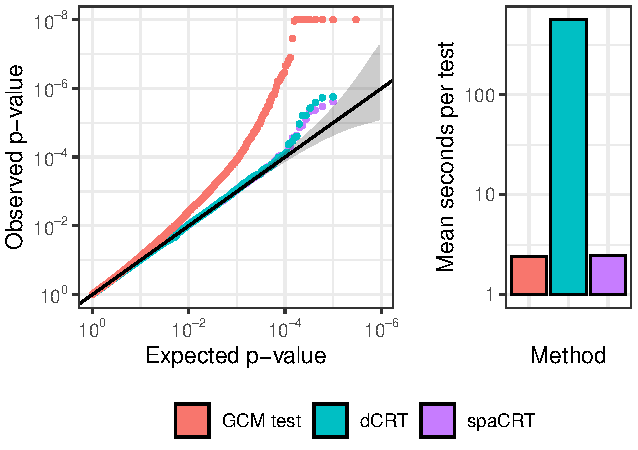
\includegraphics[width=0.6\textwidth]{figures-and-tables/real-data/motivating_example.pdf} 
	  \caption{\small{Comparing the Type-I error control and computation times of the proposed $\spacrt$ with other methods on the \citet{Gasperini2019a} data. Left: QQ-plot of the $p$-values under the null hypothesis. Right: Mean computation times per hypothesis, in seconds.}}
	  \label{fig:dCRT_GCM_binomial_poisson} 
  \end{figure*}
  
  \vspace{-0.2in}
  
  \paragraph{Paper outline.}
  
  We introduce our general theorem on the accuracy of the SPA for conditional tail probabilities in Section~\ref{sec:conditional-spa}. We then present the spaCRT methodology in Section~\ref{sec:spacrt}. We provide theoretical results for this methodology in Section~\ref{sec:general_results}, simulation results in Section~\ref{sec:simulation} and a real data application in Section~\ref{sec:real_data}, respectively. We conclude with a discussion in Section~\ref{sec:discussion}. 
  
  \section{The conditional SPA}\label{sec:conditional-spa}
  
  Consider a resampling-based hypothesis test using the statistic $\smash{T_n \equiv \frac{1}{n}\sum_{i = 1}^n T_{in}}$ computed based on a dataset $\mathcal D_n$. The resampling distribution of this test is $\smash{\widetilde T_n \equiv \frac{1}{n}\sum_{i = 1}^n \widetilde T_{in}}$, for some resampling mechanism generating $\widetilde T_{in}$ conditionally on the data $\mathcal D_n$. Then the $p$-value of this test can be defined as
  \begin{equation} \label{eq:resampling-p-value}
  p_n \equiv \P\left[\left.\frac{1}{n}\sum_{i = 1}^n \widetilde T_{in} \geq \frac{1}{n}\sum_{i = 1}^n T_{in}\ \right|\ \mathcal D_n \right].
  \end{equation}
  To abstract the statistical problem, let $\{W_{in}\}_{1 \leq i \leq n, n \geq 1}$ be a triangular array of random variables on a probability space $(\Omega, \mathcal F, \P)$ and let $\mathcal{F}_n \subseteq \mathcal F$ be a sequence of $\sigma$-algebras so that $\E[W_{in}|\mathcal{F}_n] = 0$ for each $(i, n)$ and $\{W_{in}\}_{1 \leq i \leq n}$ are independent conditionally on $\mathcal{F}_n$ for each $n$. For a sequence of cutoff values $w_n \in \mathcal F_n$, we will consider SPAs for the conditional tail probability:
  \begin{equation} \label{eq:tail-probability}
  p_n \equiv \P\left[\left.\frac{1}{n}\sum_{i = 1}^n W_{in} \geq w_n\ \right| \ \mathcal F_n\right],
  \end{equation}
  matching the definition~\eqref{eq:resampling-p-value} by setting $\smash{W_{in} \equiv \widetilde T_{in}}$, $w_n \equiv T_n$, and $\mathcal F_n \equiv \sigma(\mathcal D_n)$. These assumptions on $W_{in}$ encompass diverse resampling-based procedures, such as the bootstrap \citep{Efron1979} and the sign-flipping test \citep{Daniels1955}, but excluding permutation tests, which we leave for future work. In this section, we state our main results on the approximation accuracy of a conditional Lugannani-Rice \citep{Lugannani1980} SPA formula to approximate the tail probability~\eqref{eq:tail-probability} (Section~\ref{sec:main-results-spa}). We then discuss how this result relates to existing results (Section~\ref{sec:connection-spa-literatures}). In this section and throughout, we use standard asymptotic notations $O_\P,o_{\P}$, and $\Omega_\P$, whose formal definitions can be found in Appendix~\ref{sec:asymptotic-notations}.
  
  \subsection{Accuracy of the conditional saddlepoint approximation} \label{sec:main-results-spa}
  
  We first extend the definitions of sub-exponential and compactly supported random variables to the conditional setting, obtaining the \textit{conditionally sub-exponential} (CSE) and \textit{conditionally compactly supported} (CCS) conditions. 
  \begin{assumption}[CSE condition]\label{assu:cse}
  There exist $\theta_n \in \mathcal F_n$ and $\beta > 0$ such that $\theta_n=O_{\P}(1)$ and almost surely, 
  \begin{align*}
    0\leq \theta_n < \infty\quad\text{and}\quad\P[|W_{in}|\geq t\mid \mathcal{F}_n]\leq \theta_n\exp(-\beta t)\text{ for all $i,n$ and $t>0$}.
  \end{align*}
  \end{assumption}
  \begin{assumption}[CCS condition]\label{assu:ccs}
  There exist $\nu_{in} \in \mathcal F_n$ such that $\frac{1}{n}\sum_{i=1}^n \nu_{in}^4=O_{\P}(1)$ and almost surely, 
  \begin{align*}
    0\leq \nu_{in}<\infty\quad\text{and}\quad W_{in}\in[-\nu_{in},\nu_{in}]\text{ for all $i$ and $n$}.
  \end{align*}
  \end{assumption}
  The SPA is usually based on the cumulant-generating functions (CGFs) of the summands. For our purposes, we use conditional CGFs:
  \begin{equation}\label{eq:CCGF_def}
  K_{in}(s) \equiv \log \E[\exp(sW_{in})|\mathcal F_n] \quad \text{and} \quad K_n(s) \equiv \frac{1}{n}\sum_{i = 1}^n K_{in}(s).
  \end{equation}
  The first step of the SPA is to find the solution $\hat s_n$ to the \textit{saddlepoint equation}:
  \begin{equation}\label{eq:saddlepoint-equation}
  K_n'(s) = w_n.
  \end{equation}
  We denote the solution to saddlepoint equation \eqref{eq:saddlepoint-equation} as $\hat s_n$, whose existence and uniqueness Theorem~\ref{thm:unified_unnormalized_moment_conditions} below guarantees. With the solution $\hat s_n$ in hand, we define the saddlepoint approximation as follows. If we define
  \small
  \begin{align}\label{eq:lam_n_r_n_def}
	\lambda_n \equiv \hat s_n\sqrt{nK_n''(\hat s_n)}; \quad r_n \equiv
	\begin{cases}
	  \sgn(\hat s_n) \sqrt{2n( \hat s_n w_n - K_n(\hat s_n))} & \text{if } \hat s_n w_n - K_n(\hat s_n)\geq 0;\\
	  \mathrm{sgn}(\hat s_n) & \text{otherwise},
	\end{cases}
	\end{align}
  \normalsize
  then the saddlepoint approximation is given by
  \begin{equation}
  \widehat{\P}_{\text{LR}}\left[\left.\frac{1}{n}\sum_{i = 1}^n W_{in} \geq w_n\ \right|\ \mathcal{F}_n\right] \equiv 1-\Phi(r_n)+\phi(r_n)\left\{\frac{1}{\lambda_n}-\frac{1}{r_n}\right\}. \label{eq:lugannani-rice}
  \end{equation}
  When $w_n = 0$, we have $\hat s_n = \lambda_n = r_n = 0$. In this case, we take by convention that $1/0 - 1/0 \equiv 0$ in equation~\eqref{eq:lugannani-rice}, so that $\widehat{\P}_{\text{LR}} \equiv 1/2$. We also use the convention $0/0\equiv1$. The approximation $\widehat{\P}_{\text{LR}}$~\eqref{eq:lugannani-rice} is a direct generalization of the classical Lugannani-Rice (LR) formula \citep{Lugannani1980} to the conditional setting. The theorem below establishes the accuracy of this approximation.
  
  \begin{theorem}\label{thm:unified_unnormalized_moment_conditions}
	  Let $W_{in}$ be a triangular array of random variables that are mean-zero and independent for each $n$, conditionally on $\mathcal F_n$. Suppose either Assumption \ref{assu:cse} or Assumption \ref{assu:ccs} holds, and that
	  \begin{align}\label{eq:lower_bound_conditional_variance}
		  \frac{1}{n}\sum_{i=1}^n \E[W_{in}^2 \mid \mathcal{F}_n]=\Omega_{\P}(1).
	  \end{align}
	  Let $w_n \in \mathcal F_n$ be a sequence with $w_n \overset{\P} \rightarrow 0$. Then, there exists $\varepsilon>0$ such that the saddlepoint equation~\eqref{eq:saddlepoint-equation} has a unique and finite solution $\hat s_n \in [-\varepsilon/2, \varepsilon/2]$ with probability approaching 1 as $n \rightarrow \infty$. The explicit form of $\hat s_n$ and definition of $\varepsilon$ can be found in Appendix~\ref{sec:additional-details-spa}. Furthermore, the SPA $\widehat{\P}_{\textnormal{LR}}$ to the conditional tail probability~\eqref{eq:tail-probability} defined by equations \eqref{eq:lam_n_r_n_def} and~\eqref{eq:lugannani-rice} has vanishing relative error:
	  \begin{align}\label{eq:conclusion_saddlepoint_approximation}
		\P\left[\left.\frac{1}{n}\sum_{i = 1}^n W_{in} \geq w_n\ \right|\ \mathcal{F}_n\right] = \widehat{\P}_{\textnormal{LR}}\left[\left.\frac{1}{n}\sum_{i = 1}^n W_{in} \geq w_n\ \right|\ \mathcal{F}_n\right](1+o_{\P}(1)).
	  \end{align}
  \end{theorem}
  We make several remarks on this result.
  \begin{remark}[Generality and transparency of assumptions]\label{rmk:generality-transparency}
	While most of the existing literature is fragmented based on whether the summands $W_{in}$ are smooth or lattice, Theorem~\ref{thm:unified_unnormalized_moment_conditions} (and later Corollary~\ref{cor:unconditional_LR_formula}) unify these two cases by not making any such assumptions. The price we pay for this generality is that our guarantee~\eqref{eq:conclusion_saddlepoint_approximation} does not come with a rate, unlike most existing results. Nevertheless, we find it useful to have a single result encompassing a broad range of settings, in the same way that it is useful to have the central limit theorem in addition to the Berry-Esseen theorem. Our assumptions are not only general but also transparent. Most existing results require complicated and difficult-to-verify conditions, often stated in terms of transforms of $W_{in}$. By contrast, consider for example the Assumption~\ref{assu:cse} (sub-exponential summands) and condition~\eqref{eq:lower_bound_conditional_variance} (non-degenerate variance). These are standard and easy to understand and verify.
  \end{remark}
  
  \begin{remark}[Justification of application to resampling-based tests]
	The result~\eqref{eq:conclusion_saddlepoint_approximation} lays a solid mathematical foundation for applying the SPA to a range of resampling-based hypothesis tests with independently resampled summands, including the sign-flipping test, bootstrap-based tests, and the conditional randomization test (CRT). Even though our main focus in this paper is on the CRT, result~\eqref{eq:conclusion_saddlepoint_approximation} provides \textbf{the first rigorous justification of an SPA for the sign-flipping test} of the kind originally proposed by \citet{Daniels1955}, which is summarized as Theorem~\ref{thm:example} in Appendix~\ref{sec:sign-flipping}. 
  \end{remark}
	
  \begin{remark}[Technical challenges]
	The proof of Theorem \ref{thm:unified_unnormalized_moment_conditions} presents several technical challenges, requiring us to significantly extend existing proof techniques. One of the most significant challenges is the conditioning, which adds an extra layer of randomness to the problem. For example, the saddlepoint equation~\eqref{eq:saddlepoint-equation} is a random equation, with random solution $\hat s_n$, which we must show exists with probability approaching 1. Furthermore, the cutoff $w_n$ is random, and in particular we must handle cases depending on the realization of the sign of this cutoff. A crucial step in our proof (which follows the general structure of that of \cite{Robinson1982}) is to use the Berry-Esseen inequality, but the extra conditioning requires us to prove a new conditional Berry-Esseen theorem. Another challenge is that we allow $w_n$ to decay to zero at an arbitrary rate, which requires a delicate analysis of the convergence of the SPA formula appearing in the RHS of the result \eqref{eq:conclusion_saddlepoint_approximation}. 
  \end{remark}
  
  \begin{remark}[Assumptions on the threshold $w_n$]
  The role of the assumption $w_n = o_\P(1)$ is to guarantee the existence of a solution the saddlepoint equation beyond the case of compact support \citep{Daniels1954}. The assumption may appear restrictive at first glance, but since the rate of convergence of $w_n$ towards zero can be arbitrary, it accommodates at least two statistically interesting regimes: (a) Moderate deviation regime: $w_n=O_{\P}(n^{-\alpha}),\alpha\in (0,1/2)$ and (b) CLT regime: $w_n=O_{\P}(1/\sqrt{n})$. 
  \end{remark}
  
  \subsection{Connection to existing unconditional results}\label{sec:connection-spa-literatures}
  
  Our results are closely connected to several existing results in the literature. First, Theorem~\ref{thm:unified_unnormalized_moment_conditions} reduces to the following variant of the classical \citet{Lugannani1980} result by setting $\mathcal{F}_n \equiv \{\varnothing,\Omega\}$:
  
  \begin{corollary}\label{cor:unconditional_LR_formula}
	  Let $W_{in}$ be a triangular array of random variables that are mean-zero and independent for each $n$. Suppose that each $W_{in}$ is sub-exponential with constants $\theta, \beta > 0$, i.e. 
	  \begin{equation} \label{eq:subexponential}
	  \P[|W_{in}| \geq t] \leq \theta \exp(-\beta t) \quad \text{for all } t > 0.
	  \end{equation} 
	  Furthermore, suppose that
	  \begin{align}  \label{eq:nondegeneracy-unconditional}
	  \smash{\liminf_{n \rightarrow \infty}\ \frac{1}{n}\sum_{i = 1}^n \E[W_{in}^2] > 0.}
	  \end{align}
	  Given a sequence of cutoffs $w_n \rightarrow 0$ as $n \rightarrow \infty$, there is an $\varepsilon > 0$ such that the saddlepoint equation~\eqref{eq:saddlepoint-equation} has a unique solution $\hat s_n$ on $[-\varepsilon/2, \varepsilon/2]$ for all sufficiently large $n$. Furthermore, the unconditional SPA $\widehat{\P}_{\textnormal{LR}}$ has vanishing relative error
	  \begin{align} \label{eq:conclusion_unconditional_saddlepoint_approximation}
	  \P\left[\frac{1}{n}\sum_{i = 1}^n W_{in} \geq w_n\right] = \widehat{\P}_{\textnormal{LR}}\left[\frac{1}{n}\sum_{i = 1}^n W_{in} \geq w_n\right](1+o(1)).
	  \end{align}
  \end{corollary}
  Compared to the classical result of~\citet{Lugannani1980}, the significance of Theorem~\ref{thm:unified_unnormalized_moment_conditions} and Corollary~\ref{cor:unconditional_LR_formula} is the generality and transparency of the assumptions, as discussed in Remark~\ref{rmk:generality-transparency}. We provide another connection to the classical result of \citet{Robinson1982} in Appendix~\ref{sec:unconditional-spa-robinson}.
  
  \section{spaCRT: A resampling-free approximation to dCRT} \label{sec:spacrt}

  The conditional SPA established in Section~\ref{sec:conditional-spa} is more versatile than it appears. In this section, we demonstrate how it can be applied to a resampling-based conditional independence (CI) test, the dCRT \citep{Liu2022a}, which accounts for the presence of a potentially high-dimensional covariate vector via black-box machine learning methods. We define the CI testing problem and review the dCRT in Section~\ref{sec:background}. We  then introduce the $\spacrt$, its resampling-free approximation, in Section~\ref{sec:spacrt-methodology}.
  
  \subsection{Background: CI testing and the dCRT}\label{sec:background}

  Consider a predictor variable $\prx$, an outcome variable $\pry$, and a covariate vector $\prz \in \R^d$. Given a joint distribution $(\prx, \pry, \prz) \sim \law$, the CI null hypothesis is that the outcome is independent of the predictor, given the covariates:
  \begin{equation}\label{eq:conditional-independent-null}
  H_0: \prx \indep \pry \mid \prz. 
  \end{equation}
  Suppose that independent and identically distributed observations $(\srx_{in}, \sry_{in}, \srz_{in}) \iidsim \law_n$ are collected for $i = 1, \dots, n$, where the law $\law_n$ is allowed to vary with $n$. Denoting these observations collectively as $\srx \in \R^n$, $\sry \in \R^n$, $\srz \in \R^{n \times d}$, the CI testing problem is to test the null hypothesis~\eqref{eq:conditional-independent-null} based on the data $(\srx, \sry, \srz)$.
  
  The dCRT procedure \citep{Liu2022a} is a CI testing procedure, which was initially proposed in the context of \textit{model-X assumption} that $\law_n(\prx \mid \prz)$ is known \citep{CetL16}. However, this procedure is usually deployed in practice by learning this conditional distribution in-sample. In a prior work, we established the statistical properties of the dCRT with $\law_n(\prx \mid \prz)$ estimated in sample (\cite{Niu2022a}, reviewed in Appendix~\ref{sec:double-robustness}). In this paper, we will refer to the latter procedure as the $\dCRT$, allowing a minor abuse of terminology. Furthermore, we consider the special but still fairly general case when
  \begin{align}\label{eq:NEF}
    \law_n(\prx \mid \prz) = f(\prx \mid \theta = \theta_{n,x}(\prz)), \quad\text{where}\quad f(x|\theta)=\exp(\theta x -A(\theta))h(x)
  \end{align}
  is an exponential family with natural parameter $\theta$, natural parameter space $\R$, log-partition function $A$ and base measure $h$. Since we allow $\theta_{n,x}(\prz)$ to be arbitrary, the model~\eqref{eq:NEF} is very flexible. Given this setup, consider estimating the functions $\theta_{n,x}(\prz)$ and $\mu_{n,y}(\prz) \equiv \E_{\law_n}[\pry \mid \prz]$ by $\widehat{\theta}_{n,x}(\prz)$ and $\widehat \mu_{n,y}(\prz)$, respectively. The learning procedures for these quantities can be arbitrary, including nonparametric or black-box procedures. Setting $\widehat \mu_{n,x}(\prz) \equiv A'(\widehat{\theta}_{n,x}(\prz))$, we arrive at the test statistic 
  \begin{align}\label{eq:dCRThat}
	  T_n^{\dCRT}(X,Y,Z)
	=\frac{1}{n}\sum_{i=1}^{n}(\srx_{in}-\widehat\mu_{n,x}(\srz_{in}))(\sry_{in}-\widehat{\mu}_{n,y}(\srz_{in})).
  \end{align}
  The $\dCRT$ is obtained by comparing $T_n^{\dCRT}(\srx, \sry, \srz)$ to a null distribution obtained by resampling $\srx_{in} \mid \srz_{in}$ based on the estimated distribution $f(\ \cdot \mid \widehat \theta_{n,x}(Z_{in})).$ This procedure is summarized in Algorithm \ref{alg:dcrt-hat}. 

  \small
  \begin{center}
	  \begin{minipage}{\linewidth}
		  \begin{algorithm}[H]
			  \nonl  \textbf{Input:}  Data $(\srx,\sry,\srz)$, number of randomizations $M$. \\
			  Learn $\widehat{\theta}_{n,x}(\cdot)$ and $\widehat \mu_{n,x}(\cdot)$ based on $(\srx, \srz)$; learn $\widehat{\mu}_{n,y}(\cdot)$ based on $(\sry, \srz)$\;
			  Compute $T_n^{\dCRT}(\srx, \sry, \srz)$ as in \eqref{eq:dCRThat}\;
			  \For{$m = 1, 2, \dots, M$}{
				  Sample $\srxk^{(m)}|\srx, \sry, \srz \sim \prod_{i = 1}^n f(\ \cdot\mid\widehat{\theta}_{n,x}(\srz_{in}))$ and compute 
				  \begin{equation}
					  T_n^{\dCRT}(\srxk^{(m)}, \srx, \sry, \srz) \equiv \frac{1}{n}\sum_{i = 1}^n (\srxk^{(m)}_{in} - \widehat \mu_{n,x}(\srz_{in}))(\sry_{in} - \widehat \mu_{n,y}(\srz_{in})); \label{eq:resampled-dcrt-def}
				  \end{equation}
			  }
			  \nonl \textbf{Output:} $p$-value $\frac{1}{M+1} (1+ \sum_{m=1}^M\indicator\{T_n^{\dCRT}(\srxk^{(m)}, \srx, \sry, \srz) \geq T_n^{\dCRT}(\srx, \sry, \srz)\}).$
			  \caption{\bf $\dCRT$ procedure with exponential family for $\law_n(\prx \mid \prz)$}
			  \label{alg:dcrt-hat}
		  \end{algorithm}
	  \end{minipage}
  \end{center}
  \normalsize

  As a resampling-based procedure, the dCRT is well-equipped to handle sparse data of the kinds that motivate this work. By contrast, normality-based CI tests like the GCM test \citep{Shah2018} can have poor finite-sample performance in the presence of data sparsity, due to the slower convergence of the central limit theorem (recall Figure~\ref{fig:dCRT_GCM_binomial_poisson}); see Theorem~\ref{thm:illustrative} in Appendix~\ref{sec:finite_sample}. Despite its appeal, the dCRT can be computationally expensive for large-scale problems due to its resampling. This motivates us to develop a resampling-free approximation to this procedure.
  
  \subsection{The $\spacrt$}\label{sec:spacrt-methodology}
  
  To accelerate the dCRT, we propose the $\spacrt$, a completely resampling-free procedure with nearly identical statistical performance. If we consider the limit of the dCRT $p$-value as the number of resamples $M$ grows indefinitely, we obtain
  \begin{align}\label{eq:dCRT-p-value-limit}
  p_{\dCRT} \equiv \P\left[T_n^{\dCRT}(\widetilde{X},X,Y,Z)\geq T_n^{\dCRT}(X,Y,Z) \mid X,Y,Z\right].
  \end{align}
  We approximate this conditional tail probability via the SPA. Note that the resampled test statistic~\eqref{eq:resampled-dcrt-def} is the mean of  conditionally independent random variables:
  \begin{align*}
	T_n^{\dCRT}(\srxk^{(m)}, \srx, \sry, \srz) \equiv \frac{1}{n}\sum_{i=1}^n W_{in},\ W_{in}\equiv a_{in}(\widetilde X_{in}-\widehat{\mu}_{n,x}(Z_{in})),\ a_{in}\equiv Y_{in}-\widehat\mu_{n,y}(Z_{in}).
  \end{align*}
  Indeed, $W_{in}$ are independent, but not identically distributed, conditionally on the $\sigma$-algebra $\mathcal{F}_n \equiv \sigma(\srx,\sry,\srz)$. Thus, the dCRT $p$-value~\eqref{eq:dCRT-p-value-limit} fits the form~\eqref{eq:tail-probability}, so we may derive the conditional LR approximation~\eqref{eq:lugannani-rice} for the dCRT $p$-value and plug in expressions for the conditional CGF $K_{in}(s)$ and its derivatives under the exponential family model \eqref{eq:NEF} to obtain the $\spacrt$ procedure (Algorithm~\ref{alg:spacrt}). 

  \small
  \begin{center}
	  \begin{minipage}{\linewidth}
		  \begin{algorithm}[H]
			  \nonl  \textbf{Input:}  Data $(\srx,\sry,\srz)$. \\
			  
			  Learn $\widehat \theta_{n,x}(\cdot)$ and $\widehat \mu_{n,x}(\cdot)$ based on $(\srx, \srz)$, $\widehat{\mu}_{n,y}(\cdot)$ based on $(\sry, \srz)$\;
			  
			  Compute $T_n^{\dCRT}(\srx, \sry, \srz)=\frac{1}{n}\sum_{i=1}^{n}(\srx_{in}-\widehat\mu_{n,x}(\srz_{in}))(\sry_{in}-\widehat{\mu}_{n,y}(\srz_{in}))$\;
  
			  Find $\hat s_n$ that solves the saddlepoint equation
			  \begin{align}\label{eq:saddle_equation_nef}
				  \frac{1}{n}\sum_{i = 1}^n a_{in}\left(A'(\widehat \theta_{n,x}(\srz_{in})+a_{in}\hat s_n)-A'(\widehat \theta_{n,x}(\srz_{in}))\right)= T_n^{\dCRT}(\srx,\sry,\srz);
			  \end{align}\\
  
			  Compute $\lambda_n = \sqrt{n} \hat s_n \sqrt{\frac{1}{n}\sum_{i = 1}^n a_{in}^2A''(\widehat \theta_{n,x}(\srz_{in})+a_{in}\hat s_n)}$ and $r_n=\sgn(\hat s_n)R_n$, where
        \begin{align*}
				   R_n = \sqrt{2n\hat s_n T_n^{\dCRT} - 2\sum_{i = 1}^n (A(\widehat \theta_{n,x}(\srz_{in})+a_{in}\hat s_n)-A(\widehat \theta_{n,x}(\srz_{in}))-a_{in}\hat s_n A'(\widehat \theta_{n,x}(\srz_{in})))}
			  \end{align*}
        if the quantity in square root is non-negative; otherwise $R_n = 1$\;
			  \nonl \textbf{Output:} $\spacrt$ $p$-value
		\begin{equation} \label{eq:p_spacrt_def}
		\smash{p_{\spacrt} \equiv 1-\Phi(r_n)+\phi(r_n)\left\{\frac{1}{\lambda_n}-\frac{1}{r_n}\right\}.}
		\end{equation}
			  \caption{\bf $\spacrt$ procedure}
			  \label{alg:spacrt}
		  \end{algorithm}
	  \end{minipage}
  \end{center}
  \normalsize

  The $\spacrt$ is attractive because it is completely resampling-free. It requires the following one-time computations: fitting the estimates $\widehat \theta_{n,x}$ and $\widehat \mu_{n,y}$, calculating the test statistic $T_n^\dCRT$, and solving the saddlepoint equation~\eqref{eq:saddle_equation_nef}. The latter is a one-dimensional root-finding problem that can be solved efficiently. Indeed, since the saddlepoint equations~\eqref{eq:saddlepoint-equation} and~\eqref{eq:saddle_equation_nef} are based on the increasing function \( K_n'(s) \), binary search algorithms can be employed to find the root in logarithmic time.
  
  To exemplify the $\spacrt$ procedure, consider the case where $\prx$ is binary, as it is in single-cell CRISPR screens, one of our motivating applications.
  
  \begin{example}[Bernoulli sampling]
	Suppose $\prx\mid\prz\sim \mathrm{Ber}(\mu_{n,x}(\prz))$, and $\theta_{n,x}(\prz) = \text{logit}(\mu_{n,x}(\prz))$. Then, we have $A(\theta) = \log(1 + \exp(\theta))$. After some manipulation, the saddlepoint equation reduces to 
	  \begin{align*}
		  \frac{1}{n}\sum_{i=1}^n (\sry_{in}-\widehat{\mu}_{n,y}(\srz_{in}))(\srx_{in}-\text{expit}(\widehat \theta_{n,x}(\srz_{in})+s(\sry_{in}-\widehat{\mu}_{n,y}(\srz_{in})))=0,
	  \end{align*}
    where $\expit(x)\equiv 1/ (1+\exp(-x))$. Defining $\widetilde \mu_{n,x}(Z_{in}) \equiv \text{expit}(\widehat \theta_{n,x}(\srz_{in})+\hat s_n(\sry_{in}-\widehat{\mu}_{n,y}(\srz_{in})))$ for convenience, $\lambda_n$ and $r_n$ can be computed as 
    \begin{align*}
      \lambda_n=\hat s_n \sqrt{\sum_{i=1}^n (\sry_{in}-\widehat{\mu}_{n,y}(\srz_{in}))^2\widetilde \mu_{n,x}(Z_{in})(1-\widetilde \mu_{n,x}(Z_{in}))},
    \end{align*}
    and
	  \begin{align*}
		  r_n=\mathrm{sgn}(\hat s_n)\sqrt{2\sum_{i=1}^n \left(X_{in} \log \frac{\widetilde \mu_{n,x}(Z_{in})}{\widehat \mu_{n,x}(Z_{in})} + (1 - X_{in})\log \frac{1 - \widetilde \mu_{n,x}(Z_{in})}{1 - \widehat \mu_{n,x}(Z_{in})}\right)},
	  \end{align*}
	or simply $\text{sgn}(\hat s_n)$ if the quantity under the square root is negative. Putting these pieces together, the $\spacrt$ $p$-value can be computed as in equation~\eqref{eq:p_spacrt_def}.	
  \end{example}
  
  \section{Theoretical guarantees for the spaCRT}\label{sec:general_results}
  
  In this section, we provide a broad set of conditions under which the spaCRT approximates the dCRT well and controls Type-I error, demonstrating that the spaCRT combines computational speed with statistical accuracy. We present general results in Section~\ref{sec:spacrt-general-theory} and explore special cases in Section~\ref{sec:case_study}. 
  
  \subsection{General theory: Approximation and Type-I errors} \label{sec:spacrt-general-theory}
  
  We first state general results concerning the approximation accuracy of the $\spacrt$ $p$-value and then prove the asymptotic Type-I error control of $\spacrt$.
  
  \begin{theorem}[Approximation accuracy]\label{thm:validity_spacrt}
	Suppose there exists $S>0$ such that \textbf{one} of the following conditions holds:
	\begin{align}
	  \sup_{i}|\widehat{\theta}_{n,x}(\srz_{in})|,\ \sup_{i}|\widehat{\mu}_{n,y}(\srz_{in})| = O_{\P}(1),\  \P[\sry_{in}\in [-S,S]]=1\text{ for any }i,n\label{eq:cse_assumption}\tag{CSE};\\
	  \frac{1}{n}\sum_{i=1}^n (\sry_{in}-\widehat{\mu}_{n,y}(\srz_{in}))^4=O_{\P}(1),\ \P\left[\srxk_{in}\in [-S,S]\right]=1\text{ for any }i,n\label{eq:ccs_assumption}\tag{CCS}.
	\end{align}
	  Suppose further that the following conditions hold:
	  \begin{align}
		  |\widehat \theta_{n,x}(\srz_{in})|<\infty,|\widehat \mu_{n,y}(\srz_{in})|<\infty\text{ for any $i,n$ almost surely};\label{eq:upper_bound_theta_a} \\
		  \frac{1}{n}\sum_{i=1}^n (Y_{in}-\widehat{\mu}_{n,y}(Z_{in}))^2 A''(\widehat \theta_{n,x}(\srz_{in}))=\Omega_{\P}(1);\label{eq:lower_bound_spacrt}\\
		  T_n^{\dCRT}(\srx,\sry,\srz)\convp 0\label{eq:x_n_convergence_spacrt}.
	  \end{align}
	  Then, the saddlepoint equation~\eqref{eq:saddle_equation_nef} has a unique and finite solution $\hat s_n \in [-1/16, 1/16]$ with probability approaching 1 as $n \rightarrow \infty$. Furthermore, $\P\left[p_{\spacrt}>0\right]\rightarrow1 \text{ as }n\rightarrow\infty$ and the spaCRT $p$-value $p_{\spacrt}$ approximates the dCRT $p$-value $p_{\dCRT}$ with vanishing relative error:
	  \begin{align}\label{eq:approximation_accuracy_spacrt}
		  p_{\dCRT} = p_{\spacrt}\cdot (1+o_\P(1)).
	  \end{align}
  \end{theorem}
  
  \noindent To better understand the assumptions in Theorem \ref{thm:validity_spacrt}, we make the following remarks.
  
  \begin{remark}[Comments on conditions]\label{rmk:cutoff-regime}
    Conditions \eqref{eq:cse_assumption} and \eqref{eq:ccs_assumption} are tail conditions corresponding to Assumptions~\ref{assu:cse} and \ref{assu:ccs}, respectively. Conditions~\eqref{eq:upper_bound_theta_a} and \eqref{eq:lower_bound_spacrt} are regularity conditions. The role of the condition \eqref{eq:x_n_convergence_spacrt} is to guarantee the existence of the solution to the saddlepoint equation. This assumption allows the test statistic $T_n^{\dCRT}(\srx,\sry,\srz)$ to converge to zero in probability, \textbf{at any rate}. In particular, this condition holds under the null hypothesis and contiguous local alternatives.
  \end{remark}
  
  
  \begin{remark}[Relative error guarantee]
	  The relative error guarantee in conclusion \eqref{eq:approximation_accuracy_spacrt} is a strong result and is a direct consequence of result~\eqref{eq:conclusion_saddlepoint_approximation}. It means not only the difference of $p$-values is close to $0$ with probability approaching 1, but also the ratio of $p$-values is close to 1 with probability approaching 1. This is a particularly desirable property for approximating small $p$-values.
  \end{remark}
  
  Defining the level-$\alpha$ tests associated with the dCRT and spaCRT $p$-values:
  \begin{align*}
  \phi^{\dCRT}_{n,\alpha} \equiv \indicator(p_{\dCRT} \leq \alpha) \quad \text{and} \quad	\phi^{\spacrt}_{n,\alpha}\equiv \indicator\left(p_{\spacrt} \leq \alpha\right),
  \end{align*}
  the following theorem states that the asymptotic Type-I error control of the spaCRT follows from that of the dCRT.
  
  \begin{corollary}[Asymptotic validity of $\spacrt$]\label{cor:asymptotic_validity_spacrt}
	Suppose the assumptions of Theorem \ref{thm:validity_spacrt} hold. Fix $\alpha\in (0,1)$. If $\lim_{n\rightarrow\infty}\P_{H_0}[p_{\dCRT}\leq \alpha]\leq \alpha$, then $\lim_{n\rightarrow\infty}\P_{H_0}[p_{\spacrt}\leq \alpha]\leq \alpha$.
  \end{corollary}

  Corollary \ref{cor:asymptotic_validity_spacrt} states the asymptotic validity of $\spacrt$ given the asymptotic validity of $\dCRT$. Under the model-X assumption that $\law_n(\prx \mid \prz)$ is known exactly, the $p$-value produced by $\dCRT$ procedure is exact, i.e., $\P_{H_0}[p_{\dCRT}\leq \alpha]\leq \alpha$. Therefore, the $\spacrt$ procedure has asymptotic Type-I error control under the assumptions of Theorem \ref{thm:validity_spacrt}. We now discuss the asymptotic validity of $\spacrt$ when considering the general in-sample fit of $\law_n(\prx \mid \prz)$.
    \begin{remark}[Double robustness and asymptotic validity of $\spacrt$]\label{rmk:double-robustness}
    With in-sample fit $\lawhat_n(\prx\mid\prz)$, \citet{Niu2022a} showed that the $\dCRT$ is asymptotically equivalent to the $\GCM$ test~\citep{Shah2018} under mild conditions. The GCM test has desirable double robustness properties, which Corollary~\ref{cor:asymptotic_validity_spacrt} implies that spaCRT inherits. \citet{Shah2018} and \citet{Smucler2019} showed that the GCM test is \textit{rate and model doubly robust}, meaning that it controls Type-I error asymptotically if (1) the product of the rates at which $\mu_{n,x}(\prz)$ and $\mu_{n,y}(\prz)$ are learned is faster than $n^{-1/2}$, or (2) one of the two regression functions is estimated consistently while the other estimator converges sufficiently fast—even if its underlying model is misspecified (see details in Appendix~\ref{sec:double-robustness}). \textbf{We conclude that the spaCRT enjoys both of these double robustness properties as well, yielding a wide range of conditions under which it controls Type-I error asymptotically.} 
  \end{remark}
  
  \subsection{Case studies with modern regression techniques}\label{sec:case_study}
  
  We dedicate this section to verifying the approximation accuracy and Type-I error control of the $\spacrt$ in special cases, including those where $\pry|\prz$ is estimated using modern regression techniques. We consider low- and high-dimensional GLMs in the main text and nonparametric kernel ridge regression in Appendix~\ref{sec:theory_nonparametric_RF_classification}. 
  
  Throughout this section, we will consider the following GLMs for the data:
  \begin{align*}
	\prx|\prz\sim \mathrm{Ber}(\prx \mid \text{logit}(\mu) = \prz^\top \gamma_n)\quad\text{and}\quad \pry\mid\prz\sim f(\pry \mid \theta = \prz^\top \beta_{n}),
  \end{align*}
  for some exponential family $f(y|\theta)$ with natural parameter $\theta$ and log-partition function $A_y$, recalling equation~\eqref{eq:NEF}. The choice of logistic model for $\prx|\prz$ is mainly for theoretical convenience. In fact, the $\spacrt$ can be easily integrated with diverse models beyond just logistic regression under binary $\prx$, such as hidden Markov models, which we employ in our simulations (Section~\ref{sec:GWAS}).

  We require the following two assumptions:
  \begin{assumption}\label{assu:non_degeneracy_variance}
  $0<\inf_n\E[(\srx_{in}-\E[\srx_{in}\mid \srz_{in}])^2(\sry_{in}-\E[\sry_{in}\mid \srz_{in}])^{2}]$.
  \end{assumption}
  
  \begin{assumption}\label{assu:compact_support_Z}
	Support of $\prz\in\mathbb{R}^d$ is compact, i.e., $\|\prz\|_{\infty}\leq C_Z$ for $C_Z\in(0,\infty)$.
  \end{assumption}
  
  
  \paragraph{Low-dimensional generalized linear regression.}
  
  Suppose we are under the classical low-dimensional setup so that we write $(\srx_{in},\sry_{in},\srz_{in})=(\srx_{i},\sry_{i},\srz_{i}),\gamma_n=\gamma$ and $\beta_n=\beta$.
  
  \begin{theorem}\label{thm:low_dim_glm_spacrt}
	Suppose $\prx\indep\pry \mid \prz$, and that Assumptions \ref{assu:non_degeneracy_variance}-\ref{assu:compact_support_Z} hold. If the maximum likelihood estimates (MLEs) $\widehat{\beta},\widehat{\gamma}$ satisfy
	\begin{align}\label{eq:GLM_theta_consistency}
	  \|\widehat{\beta}-\beta\|_1=O_\P(1/\sqrt{n})\quad\text{and}\quad\|\widehat{\gamma}-\gamma\|_1=O_\P(1/\sqrt{n}),
	\end{align}
	then Theorem \ref{thm:validity_spacrt}'s conclusion holds and $\phi_{n,\alpha}^\mathrm{\spacrt}$ controls Type-I error asymptotically.
  \end{theorem}
  Note that the $\sqrt{n}$ rate condition in \eqref{eq:GLM_theta_consistency} is classical for MLEs under mild conditions.
  
  
  \paragraph{High-dimensional regression.}
   
  We now demonstrate how $\spacrt$ can be used in the presence of high-dimensional parameters, so we allow dimension of $\prz$ (as well as $\beta_n$) to grow with sample size $n$. In particular, we consider the estimators $\widehat{\beta}_n,\widehat{\gamma}_n$ for $\beta_n,\gamma_n$ obtained from the lasso estimators \citep{tibshirani1996regression} with regularization parameters $\lambda_n,\nu_n$, respectively. The definitions of these estimators are standard and can be found in Appendix~\ref{sec:proof_of_hd_glm_spacrt}. We show that the $\spacrt$ is asymptotically valid if $\beta_n$ and $\gamma_n$ are sparse enough, and if the following assumption on the covariate distribution $\prz$ holds.
  
  \begin{assumption}[Design assumption]\label{assu:design_assumption}
	Suppose the distribution of $\prz$ satisfies
	\begin{align}
	  \inf_{n} \lambda_{\min}(\E_{\law_n}[\prz\prz^\top]) &> 0;\label{eq:boundedness_eigenvalue}\\
	  \sup_{n} \sup_{\bm \eta\in\mathbb{R}^{d}, \|\bm\eta\|_2=1}\E_{\law_n}[\langle \bm \eta, \prz \rangle^4] &<\infty.\label{eq:fourth_moment_XZ}
	\end{align} 
  \end{assumption}
  
  \begin{theorem}\label{thm:high_dim_glm_spacrt}
	Suppose $\prx\indep\pry \mid \prz$ and Assumptions \ref{assu:non_degeneracy_variance}-\ref{assu:design_assumption} hold. Defining $(s_{\beta_n},s_{\gamma_n}) \equiv (\|\beta_n\|_0,\|\gamma_n\|_0)$, suppose there exists $\delta\in(0,1)$ such that
	\begin{align}
	  \max\left\{1,s_{\gamma_n},s_{\beta_n}\right\} \sqrt{\log(d)/n}\asymp n^{-\delta};\label{eq:sparsity_condition}\\
	  \sup_n\|\gamma_n\|_1<\infty,\ \sup_n\|\beta_n\|_1<\infty.\label{eq:boundedness_coefficients}
	\end{align}
	Then if we choose $\lambda_n=C_{\lambda} \sqrt{\log(d)/n}$ and $\nu_n=C_{\nu}\sqrt{\log(d)/n}$ for some universal constants $C_\lambda,C_\nu$, the conclusion of Theorem \ref{thm:validity_spacrt} holds. If, additionally, we have 
	\begin{align}\label{eq:product_sparsity_condition}
	  s_{\gamma_n}\cdot s_{\beta_n}\cdot \frac{\log(d)}{n^{1/2}}=o(1),
	\end{align}
	then $\phi_{n,\alpha}^\mathrm{\spacrt}$ is asymptotically valid, i.e. $\lim_{n\rightarrow\infty}\E[\phi_{n,\alpha}^{\spacrt}]=\alpha$ for any $\alpha\in(0,1)$. 
  \end{theorem}
  
  Let us comment on the assumptions required. Assumption \ref{assu:design_assumption} imposes constraints on the covariate distribution, which are commonly required in high-dimensional regression \citep{Wainwright2019}. Condition \eqref{eq:sparsity_condition} regulates the growth rates of $s_{\gamma_n},s_{\beta_n},d$ and $n$. Note that the $\asymp$ symbol in this condition denotes the same order of growth; it is formally defined in Appendix~\ref{sec:asymptotic-notations}. The boundedness condition \eqref{eq:boundedness_coefficients} is a relatively mild condition required to show the almost sure convergence of $\widehat{\mu}_{n,y}(\cdot), \widehat{\theta}_{n,x}(\cdot)$ in verifying condition \eqref{eq:upper_bound_theta_a}. Condition~\eqref{eq:product_sparsity_condition} requires that the product of the sparsity levels of $\beta_n$ and $\gamma_n$ is small enough, reflecting the double robustness of $\spacrt$ (Remark~\ref{rmk:double-robustness}).
  
  \section{Application to simulated data with high sparsity}\label{sec:simulation} 
  
  As discussed in Section \ref{sec:introduction}, the $\spacrt$ is particularly useful for the analysis of sparse data. We demonstrate the advantages of $\spacrt$ in this context via two simulation studies, inspired by single-cell CRISPR screens analysis (Section~\ref{sec:CRISPR-screens}) and GWAS for a rare disease and rare genetic variants (Section~\ref{sec:GWAS}). We present additional simulation results on unbalanced classification using random forests in Appendix~\ref{sec:simulation_nonparametric_RF_classification}. Code to reproduce all analyses in this section and the next is available at \href{https://github.com/Katsevich-Lab/spacrt-manuscript}{github.com/Katsevich-Lab/spacrt-manuscript}.
  
  \subsection{Single-cell CRISPR screens analysis}\label{sec:CRISPR-screens}
  
  Single-cell CRISPR screens pair genetic perturbations with single-cell gene expression measurements to identify the effects of perturbed genomic elements on gene expression \citep{Dixit2016,Adamson2016}. The perturbation presence and gene expression data produced by these assays tend to be sparse (Appendix~\ref{sec:source_sparsity_CRISPR}), creating the analysis challenges described in the introduction.

  \paragraph{Simulation setup:}
  
  While single-cell CRISPR screens can simultaneously measure the effects of thousands of perturbations on tens of thousands of genes, we focus our simulation study on testing for association within a single perturbation-gene pair. In conjunction with using the stricter significance threshold of $\alpha = 0.005$ that could arise from a multiplicity correction, this setup already captures the relevant statistical phenomena of interest (see also Appendix~\ref{sec:additional_simulation_results_CRISPR} for results in a multiple testing setting). To simulate single-cell CRISPR screen data for a given perturbation-gene pair, let $\prx \in \{0,1\}$, $\pry \in \N$, and $\prz \in \R$ represent the indicator of perturbation presence, gene expression, and a single covariate with a confounding effect in a given cell. We observe these variables in each of $n$ cells. We model $\prx\mid\prz$ and $\pry\mid\prz$ as logistic and negative binomial regressions, respectively \citep{Gasperini2019a,Katsevich2020c,Barry2024}. The latter modeling choice is quite common not just in single-cell CRISPR screen analysis but in single-cell RNA-seq analysis more broadly \citep{Huang2018, Svensson2020,Sarkar2020}. We arrive at the model
  \begin{align}\label{eq:simulation-model-CRISPR-screens}
	\bm Z\sim N(0,1); \	\bm X \mid \bm Z\sim \textnormal{Ber}(\text{logit}(\mu) = \gamma_0+\bm Z);\\
   \bm Y \mid \bm X,\bm Z\sim \textnormal{NB}(\log(\mu) = \beta_0+\rho\bm X+\bm Z,r),
  \end{align}
  where $r > 0$ is the \textit{size parameter} controlling the overdispersion of the negative binomial distribution. The parameters $\gamma_0$ and $\beta_0$ control the proportion of cells with perturbations and the mean expression of the gene, respectively, and therefore control the sparsity level of $\srx$ and $\sry$. The parameter $\rho$ controls the strength of the signal, i.e., the dependence of $\pry$ on $\prx$ conditionally on $\prz$. Therefore, $\rho = 0$ and $\rho \neq 0$ correspond to the null and alternative hypotheses, respectively. We note that selecting the parameters $(\gamma_0,\beta_0)$ yields $\srx$ and $\sry$ whose sparsity levels closely resemble those observed in real data (see Appendix~\ref{sec:simulation_methods_CRISPR_screens} for details).
  
  
  \paragraph{Methodologies compared:}
  
  
  We compare four tests: $\spacrt,\dCRT,\GCM$ test and the negative binomial score test (we defer detailed method definitions to Appendix~\ref{sec:simulation_methods_CRISPR_screens}). We use $M=10,000$ resamples for $\dCRT$ to obtain accurate $p$-values.  
  
  \paragraph{Simulation results:}
  
  Here, we present a representative selection of simulation results (Figure~\ref{fig:simulation-summary}). These results correspond to $r = 0.05$ and $\beta_0 = -5$, and all tests are applied at nominal level $\alpha = 0.005$. Additional results are provided in Appendix~\ref{sec:additional_simulation_results_CRISPR}. We find from Figure~\ref{fig:simulation-summary}a, which displays $p$-value distributions under the null hypothesis, that the $\spacrt$ and $\dCRT$ tests have similar $p$-value distributions, both of which are close to uniform. From Figure~\ref{fig:simulation-summary}d, we see the $p$-values from $\spacrt$ and $\dCRT$ align very well for $p$-values estimated accurately enough by $M = 10,000$ dCRT resamples, validating our approximation accuracy result (Theorem~\ref{thm:validity_spacrt}) in finite samples. For very small $p$-values (those around $10^{-4}$ or smaller), the $\dCRT$ does not yield reliable estimates due to discreteness, whereas $\spacrt$ captures $p$-values as small as $10^{-7}$. Meanwhile, the GCM test behaves too liberally for left-sided tests and too conservatively for right-sided tests, while the score test behaves too conservatively for left-sided tests and too liberally for right-sided tests. These trends are reflected in the Type-I error rates and powers in Figure~\ref{fig:simulation-summary}b,c. We remark that the $\spacrt$ and $\dCRT$ tests control Type-I error for all settings of $\gamma_0$, though both tests tend to become conservative as $\srx$ becomes sparser. Furthermore, the $\spacrt$ and $\dCRT$ are the most powerful tests among those that have Type-I error control for every parameter setting.
  \begin{figure*}[!ht]
	  \centering
	  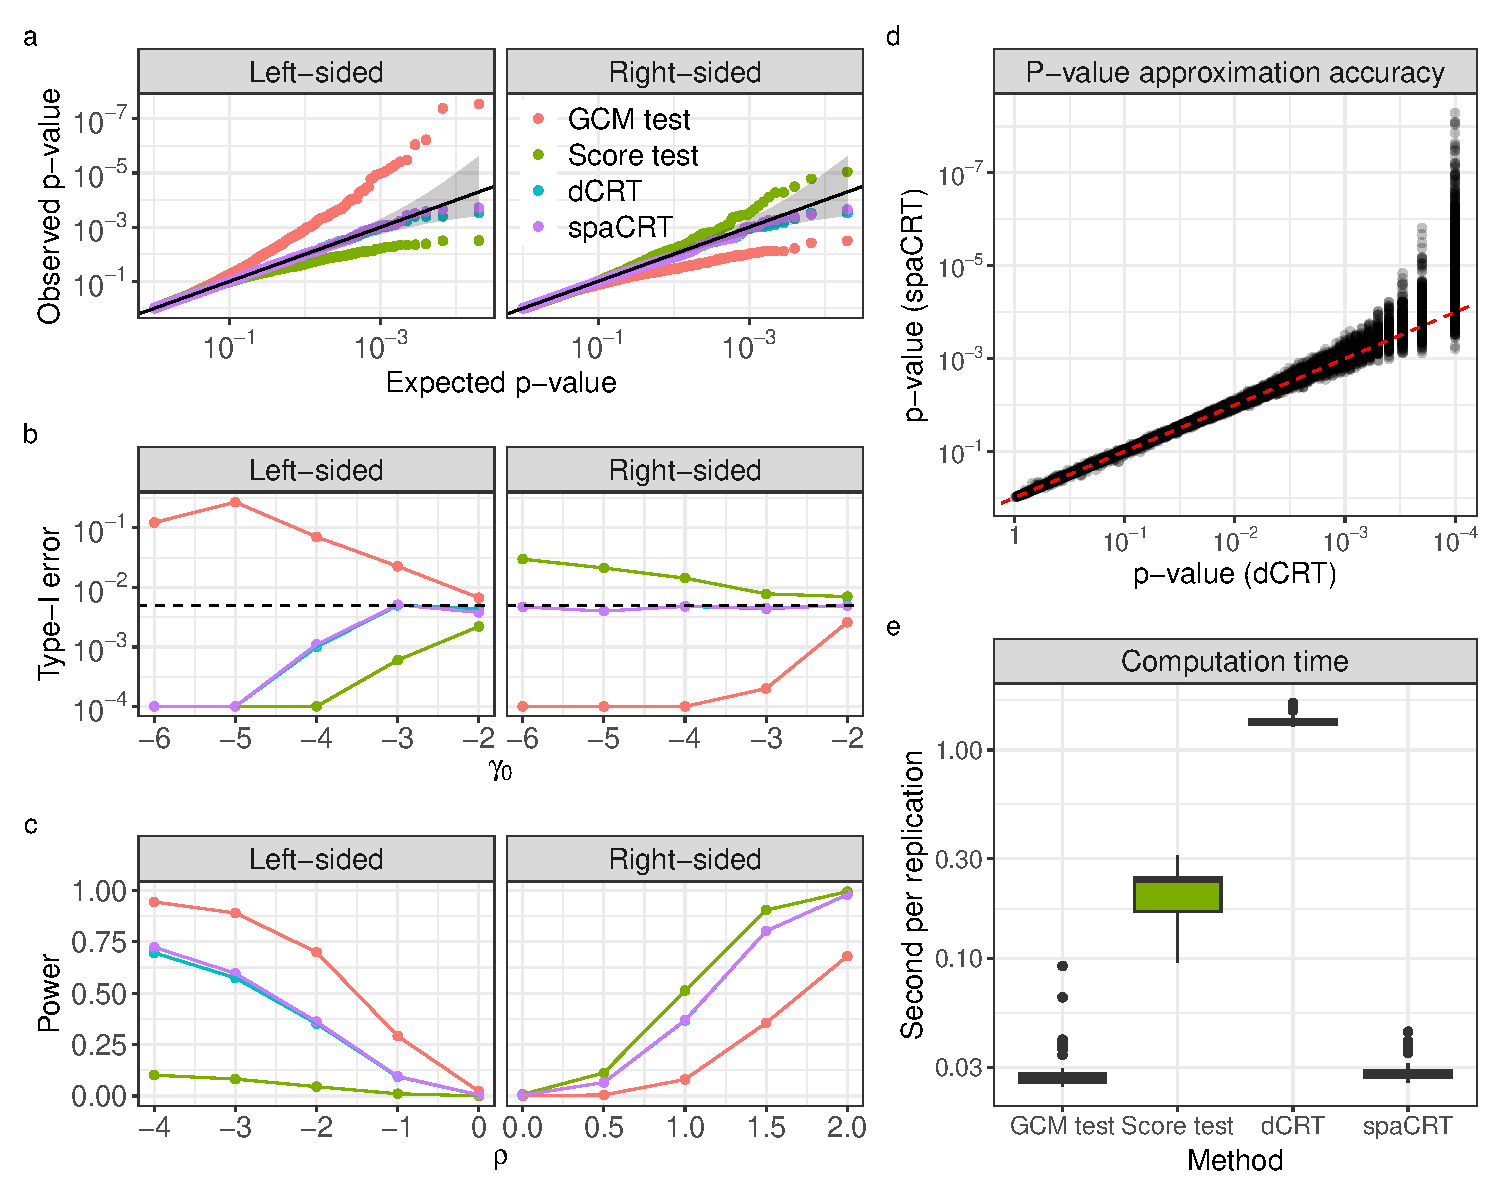
\includegraphics[width=1.0\textwidth]{figures-and-tables/simulation/NB-regression/summary/simulation-summary.pdf}
	  \caption{\small{Summary of single-cell CRISPR screen simulation results for size parameter $r = 0.05$ and the significance level $\alpha = 0.01$. (a) QQ-plots of the $p$-values obtained under the null hypothesis for $(\gamma_0, \beta_0) = (-3, -5)$. (b) Type-I error rates for $\beta_0 = -5$ as a function of the sparsity of $\srx$ ($\gamma_0$). (c) Power for $(\gamma_0, \beta_0) = (-3, -5)$ as a function of the signal strength ($\rho$). (d) Scatter plot for $p$-values comparison between $\dCRT$ and $\spacrt$ for $(\gamma_0,\beta_0,\rho)=(-3,-5,1)$. (e) Time consumed by each method across different simulation parameters. Each point in panels (b), (c), and (e) is an average over 10,000 replicates.}}
	  \label{fig:simulation-summary}
  \end{figure*}
  
  Next, we remark on how the methods' performance is impacted by the problem parameters $\gamma_0$ and $\beta_0$. As either $\srx$ or $\sry$ becomes less sparse (i.e., as $\gamma_0$ or $\beta_0$ increase), the $p$-value distributions, Type-I error rates, and powers for the GCM and score tests improve. This is to be expected, as the test statistics converge more quickly towards the standard normal distribution when the quantities being averaged are less sparse. We defer the discussion on size parameter $r$ to Appendix \ref{sec:additional_simulation_results_CRISPR}, where we show that $\dCRT$ and $\spacrt$ are less sensitive to this parameter than the GCM and score tests.
  
  
  Finally, Figure~\ref{fig:simulation-summary}e displays the computing times for the different methods in the settings considered in Figure~\ref{fig:simulation-summary}a,b,c. We see that the spaCRT and GCM test are roughly tied for fastest, the score test is roughly half an order of magnitude slower than these two, while the dCRT is more than an order of magnitude slower. 
  
  \subsection{GWAS with rare diseases and genetic variants}\label{sec:GWAS}

  The goal of genome-wide association studies (GWAS) is to identify genetic variants associated with phenotypes, such as diseases. When the genetic variants and/or the disease under investigation are rare, this makes the data highly sparse (Appendix~\ref{sec:source_sparsity_GWAS}).
  
  \paragraph{Simulation setup:}
  
  To simulate GWAS data, consider a binary disease indicator $\pry$ and a high-dimensional vector of genotypes $\prx=(\prx_1,\ldots,\prx_d)^\top\in\{0,1\}^d$ at $d$ genetic locations. While genotypes typically take values in $\{0,1,2\}$, we simplify the setup while preserving its qualitative nature by considering binary genotypes. For each location $j$, it is of interest to test for association between that location's genotype and the disease, controlling for the effects of other genetic variants. This variable selection problem has been formulated as a collection of CI testing problems \citep{sesia2019gene} fitting into our framework by considering $\prz\equiv \prx_{-j}$ as the covariates:
  \begin{align}\label{eq:variable_selection}
	H_0^j:\prx_j\indep \pry\mid \prx_{-j}, \quad j=1,\ldots,d.
  \end{align}

  We model the response as a high-dimensional logistic regression:
  \begin{align*}
	  \bm Y \mid \bm X\sim \textnormal{Ber}(\text{logit}(\mu) = \gamma_0 + \prx^\top \beta).
  \end{align*}
  Under this model, the CI null $H_0^j$ \eqref{eq:variable_selection} is equivalent to $\beta_j=0$ \citep{CetL16}. $\gamma_0$ controls the sparsity of outcome $Y$ and we consider $\{-3,-2\}$ for \textit{high} and \textit{low} sparsity (i.e. more rare and less rare disease). We model the genotype vector $\prx \in\{0,1\}^{d}$ as a \textit{hidden Markov model} (HMM), commonly adopted for this purpose \citep{scheet2006fast,marchini2007new,browning2007rapid} and reviewed in Appendix \ref{sec:HMM}. We consider two sets of HMM parameters, capturing rare and common genetic variation. We set dimension $d=500$ and sample size $n=2000$, and describe the other parameter settings to Appendix \ref{sec:simulation_methods_GWAS}. 
  
  \paragraph{Methodologies compared:}
  
  We compare four procedures: $\spacrt,\dCRT,\GCM$ test and the knockoff procedure \citep{CetL16,sesia2019gene}. All methods use the expectation-maximization (EM) algorithm of \citet{scheet2006fast} to fit the HMM distribution of $\prx$ and lasso-regularized logistic regression to fit $\pry|\prx$. The method details can be found in Appendix~\ref{sec:simulation_methods_GWAS}. We apply a two-sided test for all four methods. For $\spacrt,\dCRT$ and $\GCM$, the $p$-values are corrected for multiple testing using the Benjamini-Hochberg procedure \citep{benjamini1995controlling}. The false discovery rate (FDR) is controlled at level $q = 0.1$.
  
  \paragraph{Simulation results:}
  
  \begin{figure}[!ht]
	\centering
	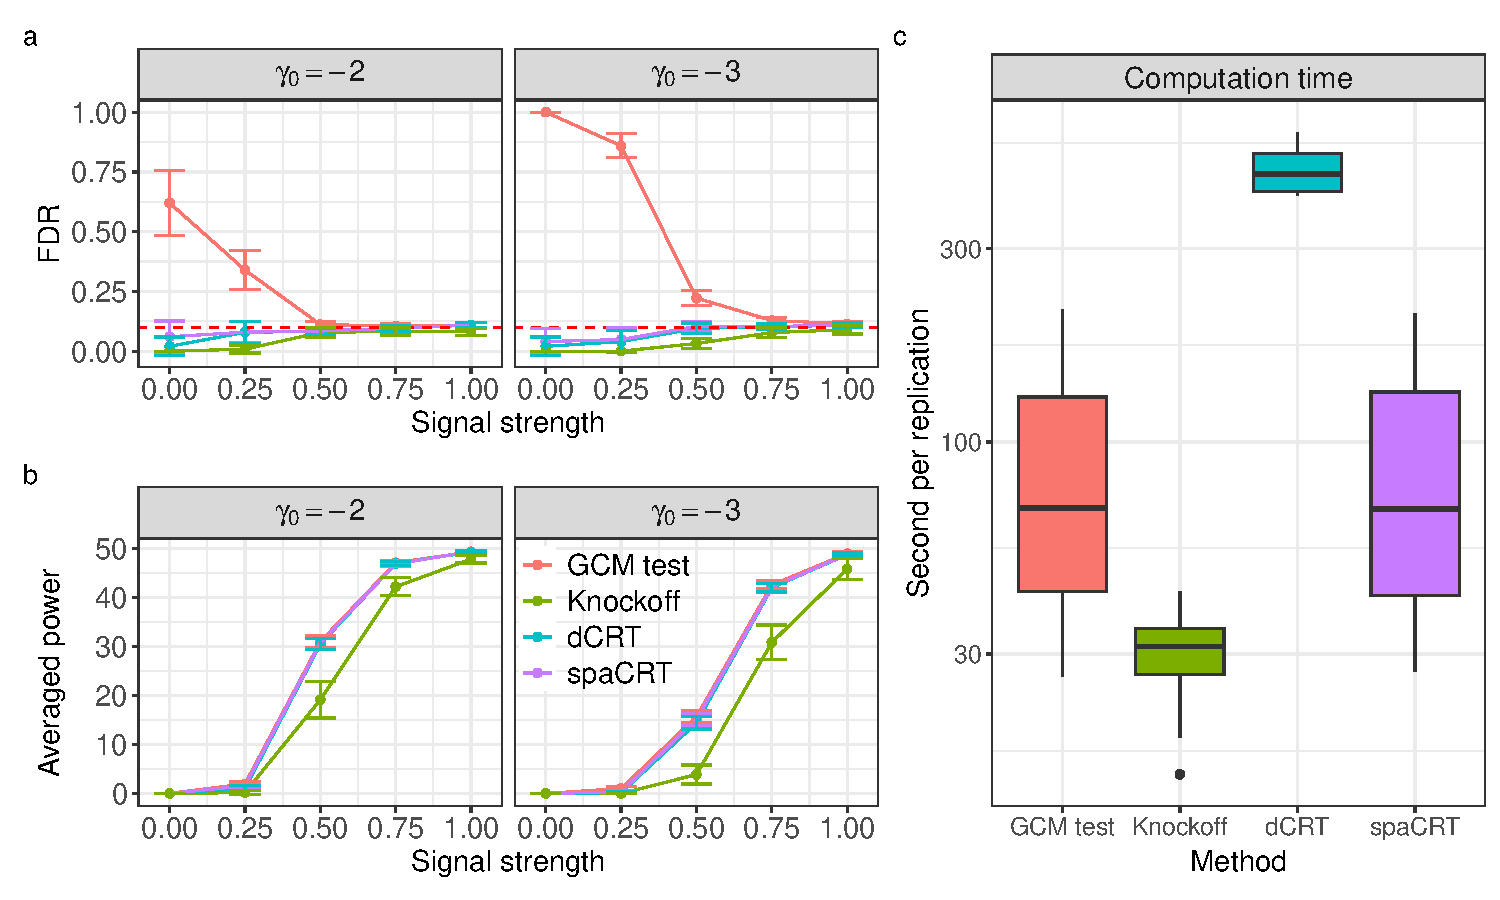
\includegraphics[width=1.0\textwidth]{figures-and-tables/simulation/HMM-variable-selection/HMM_simulation_skew_lambda.1se.pdf}
	\caption{\small{Summary of GWAS simulation results with high sparsity in data $X$. All the results are obtained with the regularization parameter $\lambda=\texttt{lambda.1se}$. (a) FDR for $\gamma_0=-3$ (high sparsity) and $\gamma_0=-2$ (low sparsity). (b) Power for the same set of $\gamma_0$. (c) Time consumed by different methods across all the varying parameters, averaged over $50$ replicates.}}
	\label{fig:simulation-summary-GWAS-skew-lambda-1se}
  \end{figure}
  We present a representative selection of simulation results (Figure~\ref{fig:simulation-summary-GWAS-skew-lambda-1se}) with high sparsity in $X$; the other results can be found in Appendix \ref{sec:simulation_results_GWAS}. Note that the knockoff procedure does not provide $p$-values but just a rejection set. Therefore, we only present the FDR plot (Figure~\ref{fig:simulation-summary-GWAS-skew-lambda-1se}a) and power plot (Figure~\ref{fig:simulation-summary-GWAS-skew-lambda-1se}b) in this simulation setup. We find from Figure~\ref{fig:simulation-summary-GWAS-skew-lambda-1se}a that the $\spacrt$ and $\dCRT$ tests have similar FDR, both of which are close to the nominal level. Meanwhile, the $\GCM$ test behaves too liberally due to high sparsity in $X$ and $Y$, although the degree of inflation is more severe when $\gamma_0=-3$. The knockoff method also controls FDR, though is conservative when the signal is weak. Figure~\ref{fig:simulation-summary-GWAS-skew-lambda-1se}b shows that $\GCM,\dCRT$ and $\spacrt$ have similar power, whereas knockoff procedure tends to be less powerful. We conjecture the latter may be due to the sensitivity of knockoffs to the distribution of $\prx$, which can affect the correlation of knockoff variables $\tilde \prx$ with the originals $\prx$, which in turn affects power. Therefore, we do not claim that the knockoff procedure is generally less powerful and postpone a more comprehensive investigation to future work. 
  
  Figure~\ref{fig:simulation-summary-GWAS-skew-lambda-1se}c shows the time consumption for different methods. Among all methods, knockoffs is the most computationally efficient, due to the fact that only one high-dimensional regression fit of $\pry|\prx,\tilde{\prx}$ is required. On the other hand, the other three methods involve $d$ regressions for $\pry|\prx_{-j},j\in[d]$ if no further acceleration is applied, not to mention the resampling required by $\dCRT$. However, we employ a \textit{tower trick} \citep{chakraborty2024doubly} to accelerate the computation of $\widehat \E[\pry|\prx_{-j}]$ for $\dCRT,\GCM$ and $\spacrt$ (Appendix \ref{sec:tower-trick}). This brings the computation time of $\spacrt$ and $\GCM$ within a factor of 2 to 3 of the knockoff procedure while being at least 4 times faster than the $\dCRT$. Part of the remaining advantage of knockoffs is due to its highly optimized implementation in the R package \texttt{SNPknock}. Finally, we note that the computational advantage of $\spacrt$ over $\dCRT$ is not as dramatic due to the relatively small multiplicity in our simulation ($d = 500$), which allows us to set $M = 5000$. Full-scale GWAS analyses involve millions of genetic variants, requiring a much larger $M$ and significantly increasing the per-test computational cost of $\dCRT$.
  
  \section{Real data analysis} \label{sec:real_data}
  
  In this section, we compare the performance of the $\spacrt$ to those of alternative methods on the analysis of the \citet{Gasperini2019a} single-cell CRISPR screen dataset. We refer reader to Appendix~\ref{sec:additional-details-real-data} for a detailed description of the dataset.
  
  \subsection{Analyses conducted}
  
  \paragraph{Hypotheses tested.} In order to assess the Type-I error and power of the methods compared, we use negative and positive control CRISPR perturbations, respectively. In particular, for Type-I error analysis, we test for association between each of the 51 negative control perturbations and each of 3,000 randomly sampled genes, for a total of 51 $\times$ 3,000 = 153,000 tests. To assess power, we test for association between each of the 754 positive control perturbations and the genes they target.
  
  \paragraph{Methods compared.} We compare essentially the same methods as in the numerical simulations (recall Section~\ref{sec:CRISPR-screens}), except we replace the dCRT with a faster variant implemented in the R package \verb|sceptre| \citep{Katsevich2020c,Barry2024}, in order to make the analysis computationally feasible. As discussed in Section~\ref{sec:relevant-literature}, the \verb|sceptre| implementation of the dCRT fits a parametric curve to the resampling distribution of the test statistic based on a smaller number of resamples. Furthermore, it is implemented in C++ for speed, unlike the other methods we consider, which are implemented in R. We apply left- and right-sided variants of each test on the negative control perturbation-gene pairs. For the positive control pairs, we apply only left-sided tests, since we are testing for a perturbation-induced decrease in gene expression.
  
  \subsection{Results}
  
  \paragraph{Type-I error.} Figure~\ref{fig:summary-real-data}a displays QQ plots of the negative control $p$-values obtained from all four methods. The two tests relying on asymptotic normality, the GCM and score tests, exhibit severe $p$-value inflation for left- and right-sided tests, respectively. This finding is consistent with our simulation results (Figure~\ref{fig:simulation-summary}). On the other hand, the $\spacrt$ and \verb|sceptre| $p$-values are well-calibrated for both left- and right-sided tests. We report the number of false discoveries on the negative control pairs in Appendix~\ref{sec:additional_table_realdata}; these results are what one would expect based on the QQ plots.
  \begin{figure*}[!ht]
	  \centering
	  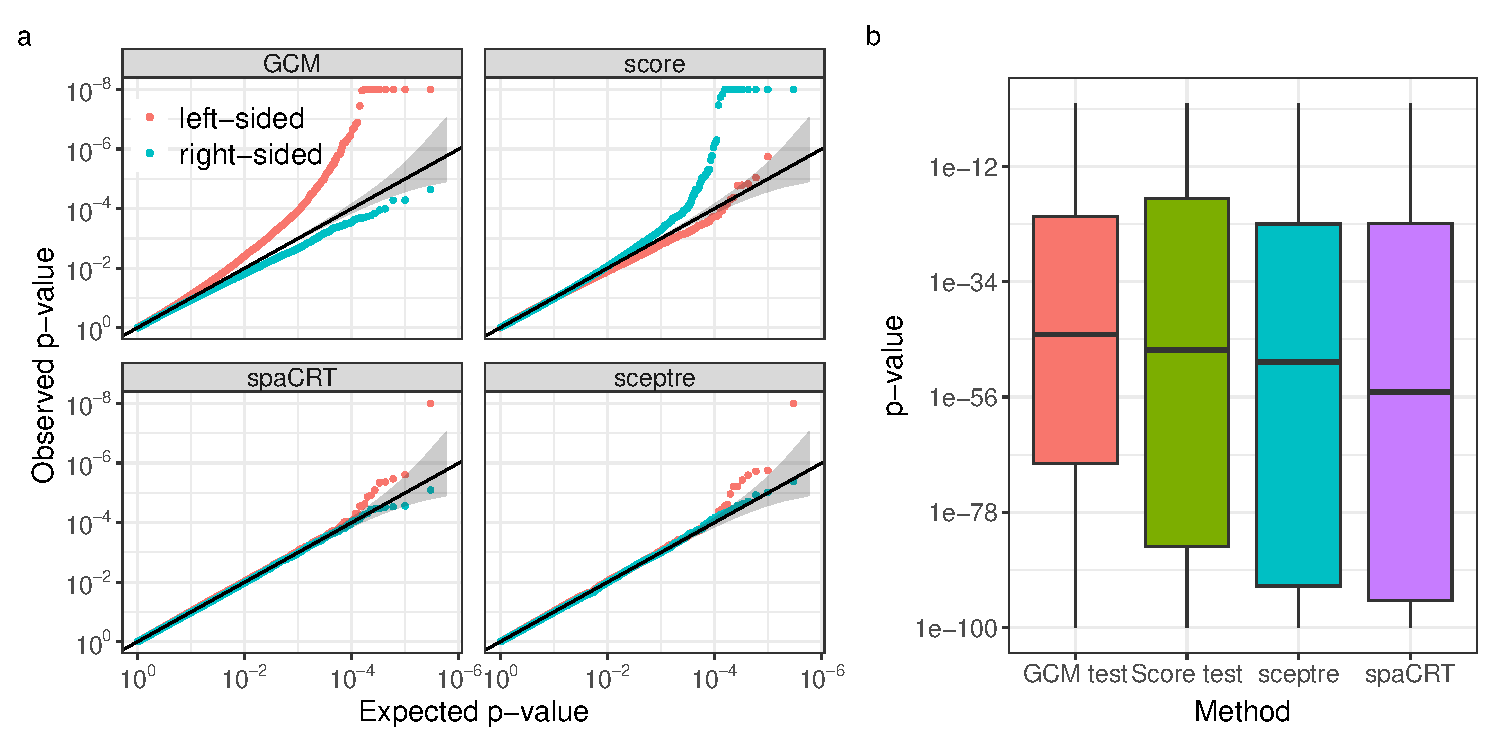
\includegraphics[width=1.0\textwidth]{figures-and-tables/real-data/combined_summary.pdf}
	  \caption{\small{Calibration and power performance on the \citet{Gasperini2019a} data. (a): Left- and right-sided $p$-values for negative control perturbation-gene pairs. (b): Left-sided $p$-values computed on the positive control perturbation-gene pairs.}}
	  \label{fig:summary-real-data}
  \end{figure*}
  
  Next, we investigate the impact of the problem sparsity on calibration. Following \citet{Barry2024}, we measure sparsity in terms of the \textit{effective sample size} $\sum_{i = 1}^n \indicator(X_{i} Y_{i} > 0)$, which measures the number of cells with a given perturbation and nonzero expression of a given gene. Table~\ref{tab:sparsity_level_ess} in Appendix~\ref{sec:sparsity_level_realdata} displays the distribution of effective sample sizes across the negative control pairs tested, showing that the effective samples sizes are vastly smaller than the number of cells, $n =$ 207,324. Furthermore, Figure~\ref{fig:qqplot_lowess} in Appendix~\ref{sec:additional_figure_realdata} stratifies the QQ plots for each method by effective sample size, focusing on those pairs with effective sample size of at most 100. As expected based on our simulation study, we find more severe miscalibration for pairs with lower effective sample sizes, especially for the GCM and score tests, and to a lesser extent for \verb|sceptre| and the $\spacrt$. We also stratified pairs based on the estimated size parameter (Figure~\ref{fig:qqplot_dispersion} in Appendix~\ref{sec:additional_figure_realdata}). As in our simulation results, the GCM and score tests exhibit more miscalibration for smaller size parameters. 
  
  \paragraph{Power.}
  
  Next, we compare the power of the four methods based on their left-sided $p$-values on the 754 positive control perturbation-gene pairs (Figure~\ref{fig:summary-real-data}b). The signal is quite strong in these positive control pairs, as evidenced by small $p$-values for all four methods. We remark that the $\spacrt$ overcomes the discreteness in the $p$-values returned by resampling-based methods such as the dCRT, delivering very small $p$-values in the presence of strong signals. Given the scale of the $p$-values, we refrain from making definitive conclusions about the relative power of the methods, but remark only that the $\spacrt$ appears at least as powerful as the alternative methods considered.
  
  
  \paragraph{Computation.}
  
  In addition to its excellent statistical performance, $\spacrt$ enjoys excellent computational performance as well. Since the \verb|sceptre| software is highly optimized, while the other methods are not, we benchmark the computational cost of our dCRT implementation (used in the numerical simulations) instead of \verb|sceptre|'s. We use $M = $ 100,000 resamples for the dCRT, given the high multiplicity of the problem. We assess runtime on 102 pairs based on two randomly sampled genes and the 51 non-targeting perturbations. We find that the $\spacrt$ is roughly as fast as the GCM test, five times faster than the score test, and 250 times faster than the dCRT.
  
  \begin{table}[!h]
\centering
\caption{\label{tab:time_comparison}Computation time per perturbation-gene pair on the Gasperini data. Times are reported in seconds.}
\centering
\begin{tabular}[t]{lrr}
\toprule
Method & Mean & Std dev\\
\midrule
GCM test & 4.0 & 1.9\\
dCRT & 1002.1 & 279.5\\
spaCRT & 4.0 & 1.9\\
Score test & 19.9 & 9.3\\
\bottomrule
\end{tabular}
\end{table}


  
  \section{Discussion} \label{sec:discussion}

  In this paper, we demonstrated that the saddlepoint approximation (SPA), previously regarded as a classical and somewhat specialized tool, can be effectively adapted to address modern, large-scale statistical inference challenges. Our primary contributions are twofold. First, we established a general conditional Lugannani–Rice result with vanishing relative error under transparent, easily verifiable tail conditions. Our approach fills decades-old theoretical gaps in the justification of SPAs for resampling-based procedures and unifies previously separate smooth and lattice cases. Second, leveraging this theoretical foundation, we developed the spaCRT, a resampling-free CI test. The spaCRT retains the excellent finite-sample statistical performance of the dCRT while reducing computational requirements by orders of magnitude (on the Gasperini data, the reduction was from years to days). Practically, researchers conducting large-scale hypothesis testing on sparse data now have access to a method (immediately deployable via the open-source \verb|spacrt| package) that balances computational efficiency with statistical accuracy, providing reliably calibrated $p$-values without the computational overhead of resampling-based procedures.

  Our work opens a number of directions for future research. Theorem~\ref{thm:unified_unnormalized_moment_conditions} can already be applied to establish conditions for the validity of existing SPAs to resampling-based hypothesis tests with conditionally independent summands, such as bootstrap tests. This result, though already quite general, can be extended in at least three ways. First, it can be extended to exchangeable yet conditionally dependent resampling schemes, in order to cover permutation tests. Second, it can be generalized to accommodate fixed cutoff sequences (in addition to its current scope of vanishing cutoff sequences), which would strengthen its applicability in extreme-tail inference. Third, it can be generalized to accommodate standardized test statistics, which are known to improve the performance of resampling-based methods \citep{Hall2010a, Chung2013, Barry2025}. With some of these extensions, the SPA can be applied to a wider range of resampling-based procedures, including the CRT with a broader class of test statistics. Finally, an adjacent question that remains open is to theoretically justify the empirically observed finite-sample improvement of the dCRT over asymptotic variants like the GCM test (Theorem~\ref{thm:illustrative} in Appendix~\ref{sec:finite_sample} proves this only in a special case).

  In conclusion, by establishing the rigorous theoretical underpinnings for the conditional SPA and embedding it within a versatile conditional independence testing framework, our work significantly advances the methodology available for high-dimensional, sparse inference problems. The spaCRT represents a substantial step forward, combining computational efficiency with rigorous statistical guarantees, thus opening avenues for further methodological development and broader application.
  
  
  \section{Acknowledgments}
  
  We are very grateful to John Kolassa, who provided valuable feedback on an earlier version of this paper. We acknowledge the Wharton research computing team for their help with our use of the Wharton high-performance computing cluster for the numerical simulations and real data analyses in this paper. This work was partially supported by NSF DMS-2113072 and NSF DMS-2310654.
  


\printbibliography


\appendix


\paragraph{Notations.}

Suppose $f$ is an infinitely differentiable function and we will use $f^{(r)}$ to denote its $r$-th derivative. 

\paragraph{Index in the supplement.}

We will use prefix $S.$ to denote the section and theoretical results number and ``E.a'' to denote the equation number. For example ``Section S.1'' or ``Conclusion (E.1)''. When there is no prefix in the index, it means the section or equation is in the main paper. For example, ``Section 2'' or ``Equation (1)''.


\section{Probability theory preliminaries}


\subsection{Asymptotic notations}\label{sec:asymptotic-notations}

We use the following standard notations regarding the asymptotic properties of a sequence of random variables $X_n$:
\begin{align*}
	&X_n = O_{\P}(1) &&\text{ if for each } \delta > 0 \text{ there is an } M > 0 \text{ s.t. } \limsup_{n \rightarrow \infty}\P[|X_n| > M] < \delta; \\
	&X_n = \Omega_{\P}(1) &&\text{ if for each } \delta > 0 \text{ there is an } \eta > 0 \text{ s.t. } \limsup_{n \rightarrow \infty}\P[|X_n| < \eta] < \delta;\\
	&X_n = o_{\P}(1) &&\text{ if } \P[|X_n| > \eta] \rightarrow 0 \text{ for all } \eta > 0.
\end{align*}

We will write $a_n \asymp b_n$ if $0<\liminf_{n\rightarrow\infty}|a_n/b_n|\leq\limsup_{n\rightarrow\infty}|a_n/b_n|<\infty$ and $a_n=o(b_n)$ if $\limsup_{n\rightarrow\infty}|a_n/b_n|=0$. Moreover, we will write $a_n\lesssim b_n$ if there exists constant $C$ such that $|a_n/b_n|\leq C$ when $n$ is large enough.


\subsection{Single probability space embedding}
To better state and understand the conditional convergence result, the following lemma helps to embed all the random variables into one big probability space.

\begin{lemma}[Embedding into a single probability space, Lemma 14 in \cite{Niu2022a}]\label{lem:embedding}
	Consider a sequence of probability spaces $\{(\P_n,\Omega_n,\mathcal{G}_n),n \geq 1\}$. For each $n$, let $\{W_{i,n}\}_{i \geq 1}$ be a collection of integrable random variables defined on $(\P_n,\Omega_n,\mathcal{G}_n)$ and let $\mathcal F_n \subseteq \mathcal G_n$ be a $\sigma$-algebra. Then there exists a single probability space $(\widetilde{\P}, \widetilde{\Omega}, \widetilde{\mathcal G})$, random variables $\{\widetilde W_{i,n}\}_{i,n \geq 1}$ on $(\widetilde{\P}, \widetilde{\Omega}, \widetilde{\mathcal G})$, and $\sigma$-fields $\widetilde{\mathcal F}_n \subseteq \widetilde{\mathcal G}$ for $n \geq 1$, such that for each $n$, the joint distribution of $(\{W_{i,n}\}_{i \geq 1}, \{\E[W_{i,n}\mid\mathcal F_n]\}_{i \geq 1})$ on $(\P_n,\Omega_n,\mathcal{G}_n)$ coincides with that of $(\{\widetilde W_{i,n}\}_{i \geq 1}, \{\E[\widetilde W_{i,n}\mid \widetilde{\mathcal F}_n]\}_{i \geq 1})$ on $(\widetilde{\P}, \widetilde{\Omega}, \widetilde{\mathcal G})$.
\end{lemma}
\noindent With the above Lemma, we are safe to state any almost sure statement which can be interpreted within one probability space. 

\subsection{Some facts about natural exponential family}

Consider the NEF with probability density function
\begin{align*}
  f(x|\theta)=h(x)\exp(\theta x-A(\theta)).
\end{align*}
Then there is one-to-one correspondence between the moments of the random variable from NEF and the derivative of the log-partition function $A(\theta)$. We summarise the relationship in the following Lemma.

\begin{lemma}[Chapter 1.2 in \cite{Efron2022}]\label{lem:moment_logpartition}
  Suppose $X\sim f(x|\theta)$ then the following identities hold:
  \begin{enumerate}
    \item $\E[X]=A'(\theta)$;
    \item $\E[X^2]-(\E[X])^2=A''(\theta)$;
    \item $\E[(X-\E[X])^3]=A^{(3)}(\theta)$;
    \item $\E[(X-\E[X])^4]-3\left(\E[(X-\E[X])^2]\right)^2=A^{(4)}(\theta)$.
  \end{enumerate}
\end{lemma}

\subsection{Preliminaries on regular conditional distribution}\label{sec:RCD_preliminary}

To better understand the argument involving conditional distribution, we briefly discuss the basic definition of regular conditional distribution (RCD). Let $\mathcal{B}(\mathbb{R}^n)$ be the Borel $\sigma$-algebra on $\mathbb{R}^n$ and $\Omega,\mathcal{F}_n$ be the sample space and a sequence of $\sigma$-algebras. For any $n\in\mathbb{N}_+,\kappa_n:\Omega\times \mathcal{B}(\mathbb{R}^n)$ is a regular conditional distribution of $W_n\equiv (W_{1n},\ldots,W_{nn})^\top$ given $\mathcal{F}_n$ if 
\begin{align*}
	\omega\mapsto \kappa_n(\omega,B) \text{ is measurable with respect to $\mathcal{F}_n$ for any fixed $B\in\mathcal{B}(\mathbb{R}^n)$};
	&
	\\
	B\mapsto \kappa_n(\omega,B) \text{ is a probability measure on }(\mathbb{R}^n,\mathcal{B}(\mathbb{R}^n));
	&
	\\
	\kappa_n(\omega,B)=\P[(W_{1n},\ldots,W_{nn})\in B|\mathcal{F}_n](\omega),\text{ for almost all }\omega\in\Omega\text{ and all }B\in\mathcal{B}(\mathbb{R}^n).&
\end{align*}
The following lemma from \cite[Theorem 8.37]{Lista2017} ensures that the general existence of $\kappa_{n}$.
\begin{lemma}[Theorem 8.37 in \cite{Lista2017}]\label{lem:Klenke_Thm_8.37}
  Suppose $(\Omega,\mathcal{G},\P)$ is the Probability triple. Let $\mathcal{F}\subset \mathcal{G}$ be a sub-$\sigma$-algebra. Let $Y$ be a random variable with values in a Borel space $(E,\mathcal{E})$ (for example, $E$ is Polish, $E=\mathbb{R}^d$). Then there exists a regular conditional distribution $\kappa_{Y,\mathcal{F}}$ of $Y$ given $\mathcal{F}$.
\end{lemma}
\noindent Result from \cite[Theorem 8.38]{Lista2017} guarantees that the conditional expectation and the integral of measurable function with respect to regular conditional distribution are almost surely same.

\begin{lemma}[Modified version of Theorem 8.38 in \cite{Lista2017}]\label{lem:Klenke_Thm_8.38}
  Let $X$ be a random variable $(\Omega,\mathcal{G},\mathbb{P})$ with values in a Borel space $(E,\mathcal{E})$. Let $\mathcal{F}\subset \mathcal{G}$ be a $\sigma$-algebra and let $\kappa_{X,\mathcal{F}}$ be a version of regular conditional distribution of $X$ given $\mathcal{F}$. Further, let $f:E\rightarrow\mathbb{R}$ be measurable and $\E[|f(X)|]<\infty$. Then we can define a version of the conditional expectation of $f(X)$ given $\mathcal{F}$ as:
  \begin{align*}
    \E[f(X)|\mathcal{F}](\omega)=\int f(x)\mathrm{d}\kappa_{X,\mathcal{F}}(\omega,x),\ \forall \omega \in\Omega.
  \end{align*}
\end{lemma}


\subsection{A version of conditional expectation}

In this paper, we will use RCD to fix a version of the conditional expectations used in the paper. Suppose $\kappa_{in}:\Omega\times \mathcal{B}(\mathbb{R})$ is a version of the RCD of $W_{in}$ given $\mathcal{F}_n$ and $\kappa_{n}:\Omega\times \mathcal{B}(\mathbb{R}^n)$ is a version of the RCD of $W_n\equiv (W_{1n},\ldots,W_{nn})^\top$ given $\mathcal{F}_n$. The conditional independent assumption can be formulated as 
\begin{align*}
	\kappa_{n}(\omega,B)=\prod_{i=1}^n \kappa_{in}(\omega,B_i),\ B=B_1\times\ldots\times B_n,\ \forall B_1,\ldots,B_n\in \mathcal{B}(\mathbb{R}),\ \forall \omega\in \Omega.
\end{align*}
Define the tilted RCD:
\begin{align*}
	\frac{\mathrm{d}\kappa_{in,s}(\omega,x)}{\mathrm{d}\kappa_{in}(\omega,x)}\equiv \frac{\exp(sx)}{\int \exp(sx)\mathrm{d}\kappa_{in}(\omega,x)},\ \frac{\mathrm{d}\kappa_{n,s}(\omega,x)}{\mathrm{d}\kappa_{n}(\omega,x)}\equiv\prod_{i=1}^n \frac{\exp(sx)}{\int \exp(sx)\mathrm{d}\kappa_{in}(\omega,x)},\ \forall \omega\in\Omega.
\end{align*}

Given tilting parameter $s$, define measure $\P_{in,s}$ and $\P_{n,s}$ on the measurable space $(\Omega, \mathcal F)$ via 
\begin{align*}
	\frac{\mathrm{d}\P_{in,s}}{\mathrm{d}\P} \equiv \frac{\exp(s W_{in})}{\E[\exp(s W_{in})|\mathcal F_n]}\quad\text{and}\quad \frac{\mathrm{d}\P_{n,s}}{\mathrm{d}\P}\equiv \prod_{i = 1}^n\frac{\mathrm{d}\P_{in,s}}{\mathrm{d}\P}.
\end{align*}
For any measurable function $f:\mathbb{R}\mapsto\mathbb{R}$ and $g:\mathbb{R}^n\mapsto\mathbb{R}$, we define the conditional expectation under original measure $\P$, tilted measure $\P_{in,s}$ and $\P_{n,s}$ respectively as
\begin{align}
	\E[f(W_{in})|\mathcal{F}_n](\omega)
	&\label{eq:def_conditional_expectation}
	\equiv \int f(x)\mathrm{d}\kappa_{in}(\omega,x),\ \forall \omega\in\Omega,\\ 
	\E_{in,s}[f(W_{in})|\mathcal{F}_n](\omega)
	&\label{eq:def_conditional_expectation_tilted}
	\equiv\int f(x)\frac{\exp(sx)}{\int \exp(sx)\mathrm{d}\kappa_{in}(\omega,x)}\mathrm{d}\kappa_{in}(\omega,x),\ \forall \omega\in\Omega,\\
	\E_{n,s}[g(W_{n})|\mathcal{F}_n](\omega)
	&\label{eq:def_conditional_expectation_tilted_product}
	\equiv\int g(y)\left(\prod_{i=1}^n \frac{\exp(sy_i)}{\int \exp(sy_i)\mathrm{d}\kappa_{in}(\omega,y_i)}\right)\mathrm{d}\kappa_{n}(\omega,y),\ \forall \omega\in\Omega
\end{align}
where $x\in\mathbb{R},y\in\mathbb{R}^n$. The above results provide a version of conditional expectation via RCD. We refer the guarantee of existence of RCD and the validity of the above definition for conditional expectation to Theorem \ref{lem:Klenke_Thm_8.37} and \ref{lem:Klenke_Thm_8.38}.

\section{An introduction to HMM}\label{sec:HMM}


\subsection{Generating genetic variable from multinomial HMM}\label{sec:gen_snp}

Consider matrix $X\in\mathbb{R}^{n\times p}$ with i.i.d. rows following the law of $\prx\in\{0,1\}^p$. Each variable of $\prx$, $\prx_j$, can be thought as a copy inherited from either paternal side or maternal side. Multinomial HMM (mHMM) is a mathematical model to model $\prx_j$ because of its probabilistic structure mimicking the hereditary nature. Before introducing the mHHM, let us first define a multinomial Markov chain (mMC) as follows:

\begin{definition}[Multinomial Makrov chain]\label{def:Markov_chain}
	We say a random variable $\pru\in\{0,1,\ldots,K\}^p$ follows a multinomial Markov Chain distribution, $\pru\equiv (\pru_1,\ldots,\pru_p)^\top \sim \text{mMC}(q,Q)$, if 
	\begin{align*}
		\pru_1\sim q\quad\text{and}\quad \pru_{j}|\pru_{j-1}\sim Q(\cdot|\pru_{j-1}),
	\end{align*}
	where $q$ is some multinomial distribution supported on $\{0,1,\ldots,K\}$ and $Q(\cdot|\cdot)\in\mathbb{R}^{K\times K}$ is a transition matrix so that $Q(\cdot|\pru_{j-1}=u)$ is a transition distribution given the observation $\pru_{j-1}$ is $u\in\{1,\ldots,K\}$.
\end{definition}
Then we consider the following definition for mHMM:
\begin{definition}[mHMM]\label{def:mhhm}
	Consider a $p$-dimensional random variable $\bm X\in\{0,1\}^p$. We say $\bm X\sim \text{mHMM}(\pru(q,Q),e)$ is an observation from a multinomial hidden Markov model with a latent \textit{multinomial Markov chain} $\bm U\equiv (\pru_1,\ldots,\pru_p)^\top \sim \text{mMC}(q,Q)$ and a multinomial emission distribution $\bm X_j|\pru_j\sim e$. In particular, we denote $\P[\bm X_j=x_j|\pru_j=u_j]\equiv e(x_j|u_j)$.
\end{definition}
\noindent In particular, we assume $\prx\equiv (\prx_1,\ldots,\prx_p)^\top$ is generated from a mHMM:
\begin{align*}
	\prx\sim \text{mHMM}(q,\pru(Q,e)).
\end{align*}
The graphical illustration of the latent DGP for observed genetic variable $\prx=(\prx_1,\ldots,\prx_p)^\top$ is shown in Figure \ref{fig:HHM}.

\begin{figure}[!ht]
	\centering
	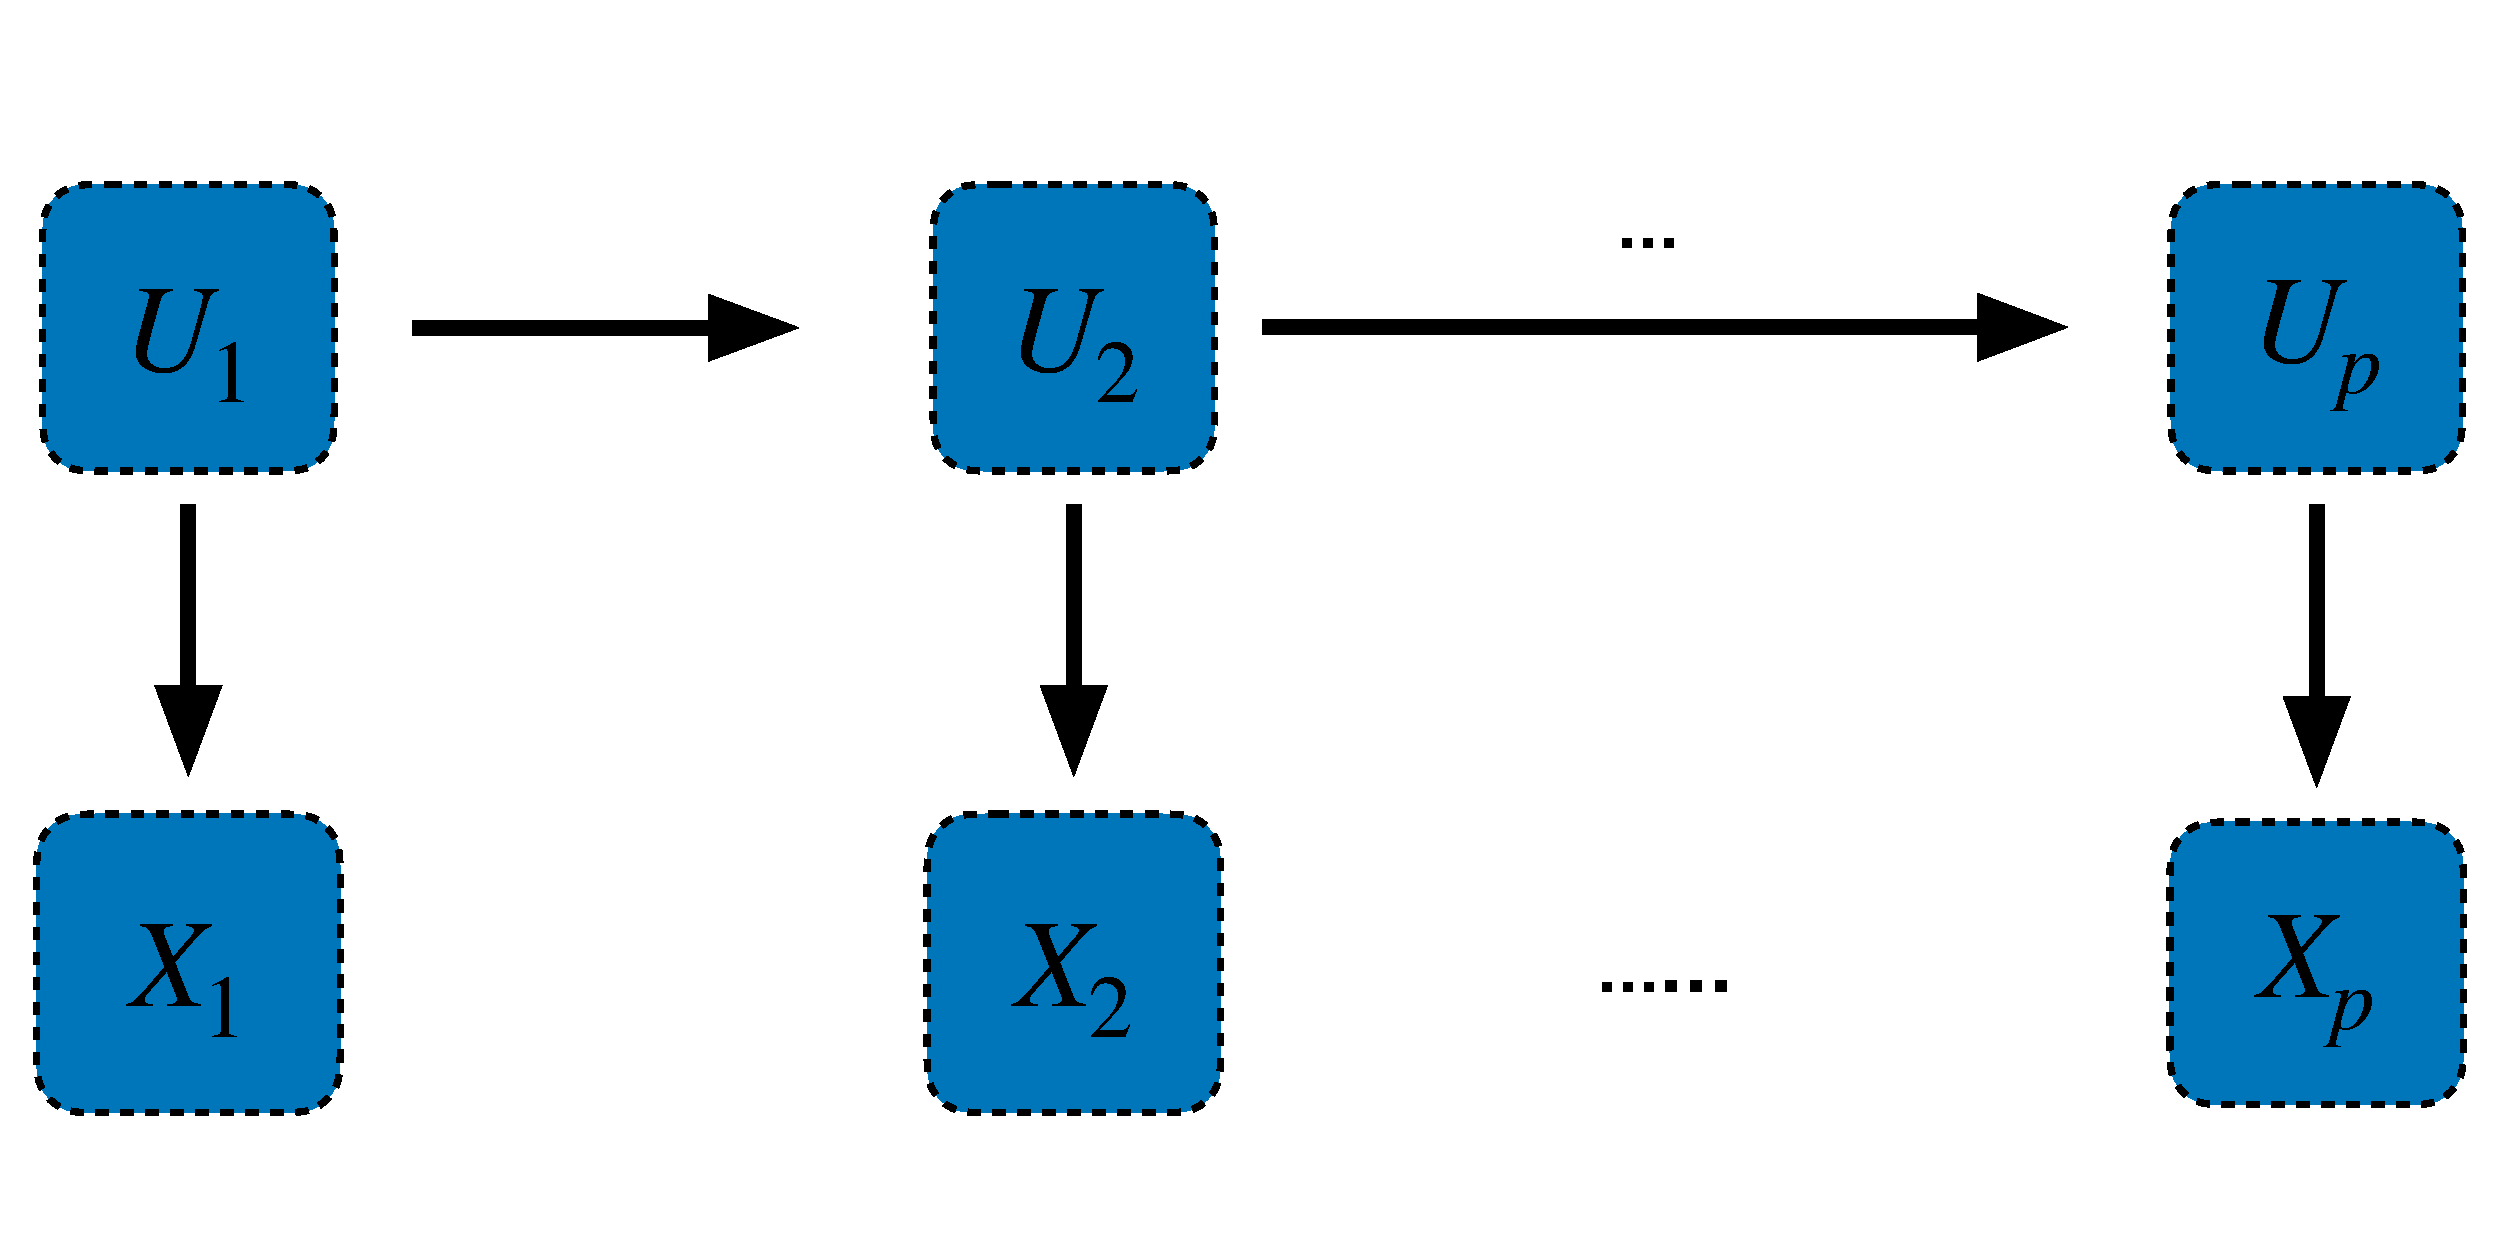
\includegraphics[width=0.7\textwidth]{figures-and-tables/HMM/mHHM.pdf}
	\caption{Graphical illustration of a multinomial hidden Markov model. Dashed rounded rectangles: unobserved variables.}\label{fig:HHM}
\end{figure}
\noindent The following identities can be easily obtained:
\begin{align}
	\P[\prx_j,\pru_{j+1}|\pru_j]
	&\label{eq:factorization}\tag{CI} 
	=\P[\prx_j|\pru_j]\P[\pru_{j+1}|\pru_j];\\
	\P[\prx_{j-1},\pru_j|\pru_{1:(j-1)},\prx_{1:(j-2)}]
	&\label{eq:Markov}\tag{Markov}
	=\P[\prx_{j-1},\pru_{j}|\pru_{j-1}],
\end{align}
where we use $\pru_{1:j}$ to denote $(\pru_1,\ldots,\pru_j)^\top\in\mathbb{R}^j$ and same notation is applied to $\prx_{1:j}$.

\subsection{Computing conditional distribution-related quantities}\label{sec:computing_conditional_quantities}

After the joint distribution $\prx$ has been estimated from fitting the mHMMs, we can compute the conditional distribution $\prx_j|\prx_{-j}$ for any $j\in[p]$ with the estimated parameters. We will dedicate this section to discussing how the conditional expectation, conditional cumulant generating function (CCGF) and its derivatives, required by the $\spacrt$ method, can be computed. We first boil these quantities down to the conditional probability $\P[\prx_j=x_j|\prx_{-j}=x_{-j}]$, where $x_{-j}\equiv (x_1,\ldots,x_{j-1},x_{j+1},\ldots,x_p)^\top\in\mathbb{R}^{p-1}$. Then we will show how the conditional probability can be computed using forward-backward algorithm. For the ease of notation, we now define for $x_{-j}\in \mathbb{R}^{p-1}$ and $t\in\mathbb{R}$,
\begin{align*}
	p(x_j,x_{-j})\equiv \P[\prx_j=x_j|\prx_{-j}=x_{-j}]\quad\text{and}\quad D(t,x_{-j})\equiv \E[\exp(t\prx_j)|\prx_{-j}=x_{-j}].
\end{align*}
\begin{enumerate}
	\item\textbf{Conditional expectation:} For any given $x_{-j}\in\mathbb{R}^{p-1}$, we can compute
	\begin{align*}
		\E[\prx_j|\prx_{-j}=x_{-j}]=p(1,x_{-j})+2\cdot p(2,x_{-j}).
	\end{align*}
	
	\item\textbf{Function value and derivatives of CCGF:} $\spacrt$ method requires the knowledge of the CCGF function and its derivatives up to second order. Then we can compute
	\begin{align*}
		D(t,x_{-j})=p(0,x_{-j})+\exp(t)p(1,x_{-j})+\exp(2t)p(2,x_{-j}).
	\end{align*}
	Thus we can compute the CCGF value:
	\begin{align*}
		K(t,x_{-j})
		&
		\equiv\log\E[\exp(t\prx_j)|\prx_{-j}=x_{-j}]=\log(D(t,x_{-j}))\quad\forall t\in\mathbb{R}.
	\end{align*}
	Then we compute the first derivative of CCGF:
	\begin{align*}
		\nabla_t K(t,x_{-j})=\frac{\exp(t)p(1,x_{-j})+2\exp(2t)p(2,x_{-j})}{D(t,x_{-j})}
	\end{align*}
	and the second derivative of CCGF:
	\begin{align*}
		\nabla_t^2 K(t,x_{-j})=\frac{\exp(t)p(1,x_{-j})+4\exp(2t)p(2,x_{-j})}{D(t,x_{-j})}-\big[\nabla_t K(t,x_{-j})\big]^2.
	\end{align*}
\end{enumerate}

Thus from the above computation, we know it is sufficient to compute the conditional probability $p(x_j,x_{-j})$. In fact, the following Proposition shows that it can be computed iteratively. To state the Proposition, we need to introduce necessary notation. For $u,\bar u\in\{0,1,\ldots,K\} $ and $x\in\{0,1\}^p$, we define 
\begin{align}
	A_j(u,x)\equiv \P[\prx_{1:(j-1)}=x_{1:(j-1)},\pru_j=u],\ A_1(u,x)\equiv \P[\pru_1=u];\label{eq:def_A}\\
  B_j(u,x)\equiv \P[\prx_{(j+1):p}=x_{(j+1):p}|\pru_j=u],\ B_p(u,x)\equiv1.\label{eq:def_B}
\end{align}

\begin{proposition}[Iterative computation of $p(x_j,x_{-j})$]\label{prop:conditional_prob}
	Suppose $\prx\sim \text{mHMM}(\pru(q,Q),e)$. Then we have
	\begin{align}\label{eq:conditional_prob_A_B}
		p(x_j,x_{-j})=\frac{\sum_{\bar u\in\{0,1,\ldots,K\}}e(x_j|\bar u)\cdot A_j(\bar u,x)\cdot B_j(\bar u,x)}{\sum_{\bar u\in \{0,1,\ldots,K\}}A_j(\bar u,x)\cdot B_j(\bar u,x)}.
	\end{align}
	In particular, $A_j$ and $B_j$ can be computed in the following recursive manner: for any $u\in\{0,1,\ldots,K\}$ and $x\in\{0,1\}^{p}$, 
	\begin{align*}
		A_j(z,x)=\sum_{\bar u\in\{0,1,\ldots,K\}}A_{j-1}(\bar u,x)\cdot r(x_{j-1}|\bar u)\cdot Q(u|\bar u);&\\
		B_j(u,x)=\sum_{\bar u\in\{0,1,\ldots,K\}}B_{j+1}(\bar u,x)\cdot r(x_{j+1}|\bar u)\cdot Q(\bar u|u).&
	\end{align*}
\end{proposition}
The proof can be found in Appendix \ref{sec:conditional_prob}.


\subsection{Proof of Proposition \ref{prop:conditional_prob}}\label{sec:conditional_prob}

\paragraph{Proof of conclusion \eqref{eq:conditional_prob_A_B}.}

First, let us consider the following marginalization:
\begin{align*}
	&
	\P[\bm X_j=x_j|\bm X_{-j}=x_{-j}]\\
	&
	=\sum_{\bar u\in \{0,1,\ldots,K\}}\P[\prx_j=x_j|\prx_{-j}=x_{-j},\pru_{j}=\bar u]\P[\pru_j=\bar u|\prx_{-j}=x_{-j}]\\
	&\tag{\ref{eq:Markov} property}
	=\sum_{\bar u\in \{0,1,\ldots,K\}}\P[\bm X_j=x_j|\pru_{j}=\bar u]\P[\pru_j=\bar u|\bm X_{-j}=x_{-j}]\\
	&
	=\sum_{\bar u\in \{0,1,\ldots,K\}}e(x_j|\bar u)\P[\pru_j=\bar u|\bm X_{-j}=x_{-j}].
\end{align*}
Now we compute the conditional probability $\P[\pru_j=u|\bm X_{-j}=x_{-j}]$. In particular, we consider the following decomposition
\begin{align*}
	\P[\pru_j=u|\bm X_{-j}=x_{-j}]=\frac{\P[\pru_j=u,\bm X_{-j}=x_{-j}]}{\P[\bm X_{-j}=x_{-j}]}=\frac{\P[\pru_j=u,\bm X_{-j}=x_{-j}]}{\sum_{\bar u\in \{0,1,\ldots,K\}}\P[\pru_j=\bar u,\bm X_{-j}=x_{-j}]}.
\end{align*}
Thus we have 
\begin{align*}
	\P[\bm X_j=x_j|\bm X_{-j}=x_{-j}]=\frac{\sum_{\bar u\in \{0,1,\ldots,K\}}e(x_j|\bar u)\P[\pru_j=\bar u,\bm X_{-j}=x_{-j}]}{\sum_{\bar u\in \{0,1,\ldots,K\}}\P[\pru_j=\bar u,\bm X_{-j}=x_{-j}]}
\end{align*}
so that we only need to compute the probability $\P[\pru_j=u,\bm X_{-j}=x_{-j}]$. Further, we can do the following calculation 
\begin{align*}
	\P[\pru_j=u,\bm X_{-j}=x_{-j}]
	&
	=\P[\bm X_{1}=x_1,\ldots, \prx_{j-1}=x_{j-1},\pru_{j}=u]\\
	&
	\quad\times\P[\prx_{j+1}=x_{j+1},\ldots, \prx_{p}=x_{p}|\prx_{1}=x_1,\ldots, \prx_{j-1}=x_{j-1},\pru_{j}=u]\\
	&
	=\P[\prx_{1}=x_1,\ldots, \prx_{j-1}=x_{j-1},\pru_{j}=u]\\
	&\tag{\ref{eq:Markov} property}
	\quad\times \P[\bm X_{j+1}=x_{j+1},\ldots, \prx_{p}=x_{p}|\pru_{j}=u]\\
	&
	= A_{j}(u,x)\cdot B_j(u,x).
\end{align*}
The detailed derivation of $A_j(u,x)$ and $B_j(u,x)$ will be present in the next two sections.

\paragraph{Computing $A_j(u,x)$ using forward algorithm.}

We use prove-by-induction to derive $A_j(u,x)$ and the induction is on index $j$. Since $A_1(u,x)=\P[\pru_1=u]$ and we can compute:
\begin{align*}
	A_2(u,x)
	&
	=\P[\prx_1=x_1,\pru_2=u]\\
	&
	=\sum_{\bar u\in\{0,1,\ldots,K\}}\P[\pru_1=\bar u]\P[\prx_1=x_1,\pru_2=z|\pru_1=\bar u]\\
	&\tag{\ref{eq:factorization} property}
	=\sum_{\bar u\in\{0,1,\ldots,K\}}\P[\pru_1=\bar u]\P[\prx_1=x_1|\pru_1=\bar u]\P[\pru_2=u|\pru_1=\bar u]\\
	&\tag{Definition \eqref{eq:def_A}}
	=\sum_{\bar u\in\{0,1,\ldots,K\}}A_1(\bar u,x)\cdot e(x_1|\bar u)\cdot Q(u|\bar u).
\end{align*}
Then we can easily show that 
\begin{align*}
	A_j(u,x)
	&
	=\P[\prx_{1}=x_1,\ldots, \prx_{j-1}=x_{j-1},\pru_{j}=u]\\
	&
	=\sum_{\bar u\in\{0,1,\ldots,K\}}\P[\prx_{1}=x_1,\ldots, \prx_{j-2}=x_{j-2},\pru_{j-1}=\bar u]\\
	&
	\qquad\times\P[\prx_{j-1}=x_{j-1},\prz_{j}=z|\prx_{1}=x_1,\ldots, \prx_{j-2}=x_{j-2},\pru_{j-1}=\bar u]\\
	&
	=\sum_{\bar u\in\{0,1,\ldots,K\}}\P[\prx_{1}=x_1,\ldots, \prx_{j-2}=x_{j-2},\pru_{j-1}=\bar u]\\
	&\tag{\ref{eq:Markov} property}
	\qquad\times\P[\prx_{j-1}=x_{j-1},\pru_{j}=u|\pru_{j-1}=\bar u]\\
	&\tag{Definition \eqref{eq:def_A}}
	=\sum_{\bar u\in\{0,1,\ldots,K\}}A_{j-1}(\bar u,x)\cdot e(x_{j-1}|\bar u)\cdot Q(u|\bar u).
\end{align*}
With iterative computation, one can obtain the probability $A_j(u,x)$ for any $j\in[p]$ and $u\in \{0,1,\ldots,K\}$ and $x\in\{0,1\}^p$.

\paragraph{Computing $B_j(u)$ using backward algorithm.}

Using $B_p(u,x)=1$ for any $u$, we can compute 
\begin{align*}
	B_{p-1}(u,x)
	&
	=\P[\prx_{p}=x_p|\pru_{p-1}=u]\\
	&
	=\sum_{\bar u\in\{0,1,\ldots,K\}}\P[\prx_p=x_p,\pru_{p}=\bar u|\pru_{p-1}=u]\\
	&
	=\sum_{\bar u\in\{0,1,\ldots,K\}} \P[\prx_p=x_p|\pru_p=\bar u,\pru_{p-1}=u]\P[\pru_p=\bar u|\pru_{p-1}=u]\\
	&\tag{\ref{eq:Markov} property}
	=\sum_{\bar u\in\{0,1,\ldots,K\}} \P[\prx_p=x_p|\pru_p=\bar u]\P[\pru_p=\bar u|\pru_{p-1}=u]\\
	&\tag{Definition \eqref{eq:def_B}}
	=\sum_{\bar u\in\{0,1,\ldots,K\}} B_{p}(\bar u, x)\cdot e(x_p|\bar u)\cdot Q(\bar u|u).
\end{align*}
By induction, we can compute 
\begin{align*}
	B_{j}(u,x)
	&
	=\P[\bm X_{j+1}=x_{j+1},\ldots, \prx_{p}=x_{p}|\pru_{j}=u]\\
	&
	=\sum_{\bar u\in\{0,1,\ldots,K\}}\P[\bm X_{j+1}=x_{j+1},\ldots, \prx_{p}=x_{p},\pru_{j+1}=\bar u|\pru_{j}=u]\\
	&
	=\sum_{\bar u\in\{0,1,\ldots,K\}}\P[\prx_{j+2}=x_{j+2},\ldots, \prx_{p}=x_{p}|\pru_{j+1}=\bar u,\pru_{j}=u,\prx_{j+1}=x_{j+1}]\\
	&
	\qquad\times\P[\prx_{j+1}=x_{j+1},\prz_{j+1}=\bar u|\pru_{j}=u]\\
	&\tag{\ref{eq:Markov} property}
	=\sum_{\bar u\in\{0,1,\ldots,K\}}\P[\prx_{j+2}=x_{j+2},\ldots, \prx_{p}=x_{p}|\pru_{j+1}=\bar u]\\
	&\tag{\ref{eq:factorization} property}
	\qquad\times \P[\prx_{j+1}=x_{j+1}|\pru_{j+1}=\bar u]\cdot \P[\pru_{j+1}=\bar u|\pru_{j}=u]\\
	&\tag{Definition \eqref{eq:def_B}}
	=\sum_{\bar u\in\{0,1,\ldots,K\}}B_{j+1}(\bar u,x)\cdot e(x_{j+1}|\bar u)\cdot Q(\bar u|u).
\end{align*}
With iterative computation, one can obtain the probability $B_j(u,x)$ for any $j\in[p]$ and $u\in \{0,1,\ldots,K\}$ and $x\in\{0,1\}^p$.

\paragraph{Final form: combining $A_j(u,x)$ and $B_j(u,x)$.}

Now we compute the probability $\P[\pru_j=u_j,\prx_{-j}=x_{-j}]$ using the derivation in the above sections. In particular, fixing a set of value $x_{-j}$, we compute 
\begin{align*}
	\P[\pru_j=u,\prx_{-j}=x_{-j}]=\frac{A_j(u,x)\cdot B_j(u,x)}{\sum_{\bar u\in \{0,1,\ldots,K\}}A_j(\bar u,x)\cdot B_j(\bar u,x)}\quad\forall j\in[p]\quad\text{and}\quad u\in[K],
\end{align*}
where $A_j(u,x),B_j(u,x)$ can be computed iteratively as before.

\section{Additional details of Section~\ref{sec:conditional-spa}}

\subsection{Additional details of Section~\ref{sec:main-results-spa}}\label{sec:additional-details-spa}

We first discuss the existence of the conditional cumulant generating function $K_{in}(s)$ and its derivatives. Either Assumption~\ref{assu:cse} or Assumption~\ref{assu:ccs} guarantees the existence of the CGFs $K_{in}(s)$ and their derivatives in a neighborhood of the origin. This is formalized in the following lemma. 
\begin{lemma}\label{lem:finite_cgf}
Suppose Assumption~\ref{assu:cse} or Assumption~\ref{assu:ccs} holds. Then, there exists a probability-one event $\mathcal A$ and an $\varepsilon > 0$ such that, on $\mathcal A$,
\begin{align}
K_{in}(s) < \infty\quad \text{for any } s\in (-\varepsilon,\varepsilon)\ \text{and}\ \text{for all}\ i \leq n,\ n \geq 1 \label{eq:finite_cgf}
\end{align}
and 
\begin{equation}\label{eq:finite_cgf_derivatives}
	|K_{in}^{(r)}(s)| < \infty\quad \text{for any } s\in (-\varepsilon,\varepsilon)\ \text{and}\ \text{for all}\ i \leq n,\ n \geq 1, \ r \geq 1, r\in\mathbb{N},
\end{equation}
where $K_{in}^{(r)}$ denotes the $r$-th derivative of $K_{in}$.
\end{lemma}

We now explicitly define the solution to saddlepoint equation~\eqref{eq:saddlepoint-equation} $\hat s_n$. In particular, consider $\varepsilon$ given in Lemma~\ref{lem:finite_cgf}, we restrict our attention to solutions in the interval $[-\varepsilon/2, \varepsilon/2]$:
\begin{align*}
S_n\equiv \left\{s\in [-\varepsilon/2,\varepsilon/2]:K_n'(s)=w_n\right\}.
\end{align*}
It is possible, for specific realizations of $K'_n(s)$ and $w_n$, that the set $S_n$ is either empty or contains multiple elements. To make the saddlepoint approximation well-defined in these cases, we define $\hat s_n$ as follows:
\begin{equation}\label{eq:def_s_n}
\hat s_n \equiv 
\begin{cases}
\text{the single element of }S_n & \text{if } |S_n|=1; \\
\frac{\varepsilon}{2}\mathrm{sgn}(w_n) & \text{otherwise}.
\end{cases}
\end{equation}
Note that this definition ensures that $\hat s_n \in [-\varepsilon/2, \varepsilon/2]$. Also, we state a complete version of Theorem~\ref{thm:unified_unnormalized_moment_conditions} below, which includes the conditions for the existence of the saddlepoint approximation. We will prove in Section~\ref{sec:spa_proof} that, the saddlepoint equation~\eqref{eq:saddlepoint-equation} has a unique and finite solution $\hat s_n \in [-\varepsilon/2, \varepsilon/2]$ with probability approaching 1 as $n \rightarrow \infty$:
\begin{equation}
\lim_{n \rightarrow \infty} \P[|S_n| = 1] = 1.
\label{eq:unique_solution_in_probability}
\end{equation}


\subsection{A connection to Robinson's formula \citep{Robinson1982}}\label{sec:unconditional-spa-robinson}

Aside from the Lugannani-Rice formula, another tail probability estimate is proposed in \cite{Robinson1982}. In fact, we present an extension of Theorem~\ref{thm:unified_unnormalized_moment_conditions} in Proposition \ref{prop:equivalence_spa_formula} that employs a conditional variant of Robinson's formula:
  \begin{equation}
	\widehat{\P}_\text{R}\left[\left.\frac{1}{n}\sum_{i = 1}^n W_{in} \geq w_n\ \right|\ \mathcal{F}_n\right] \equiv \exp\left(\frac{\lambda_n^2-r_n^2}{2}\right)(1-\Phi(\lambda_n)).
	\label{eq:robinson-formula}
  \end{equation}
  \begin{proposition}\label{prop:equivalence_spa_formula}
	Under the assumptions of Theorem \ref{thm:unified_unnormalized_moment_conditions},   
	\begin{align}\label{eq:alternative_spa_formula}
	  \P\left[\left.\frac{1}{n}\sum_{i = 1}^n W_{in} \geq w_n\ \right|\ \mathcal{F}_n\right]=\widehat{\P}_\text{R}\left[\left.\frac{1}{n}\sum_{i = 1}^n W_{in} \geq w_n\ \right|\ \mathcal{F}_n\right](1+o_\P(1)).
	  \end{align}
  \end{proposition}
  \noindent In other words, $\widehat{\P}_\text{LR}$~\eqref{eq:lugannani-rice} is equivalent to $\widehat{\P}_\text{R}$~\eqref{eq:robinson-formula} with relative error $o_\P(1)$, linking Robinson's formula to that of Lugannani and Rice. A similar result was proved in the unconditional case by \citet{Kolassa2007}. The proof of Proposition~\ref{prop:equivalence_spa_formula} is postponed to Section~\ref{sec:proof_proposition_equivalence_spa_formula}.



\subsection{Application to sign-flipping test}\label{sec:sign-flipping}

In this section, we apply Theorem~\ref{thm:unified_unnormalized_moment_conditions} to derive and justify the validity of the Lugannani-Rice SPA for the sign-flipping test. Suppose
\begin{equation}
X_{in}=\mu_n+\varepsilon_{in}, \quad \varepsilon_{in} \indsim F_{in}, 
\label{eq:location-model-symmetric-errors}
\end{equation}
where the error distributions $F_{in}$ are symmetric, but potentially distinct and unknown. We are interested in testing 
\begin{equation}
H_{0n}:\mu_n=0 \quad \text{versus} \quad H_{1n}:\mu_n>0
\end{equation}
based on $T_n \equiv \frac{1}{n}\sum_{i=1}^n X_{in}$. Note that the SPA cannot directly be applied to approximate tail probabilities of $T_n$ because the error distributions $F_{in}$ are unknown. Instead, we can approximate the tail probability of $T_n$ by conditioning on the observed data and resampling the signs of the data. In particular, define the resamples
\begin{equation}
\widetilde X_{in} \equiv \pi_{in} X_{in}, \quad \pi_{in} \iidsim \text{Rad}(0.5),
\end{equation}
where $\text{Rad}(0.5)$ denotes the Rademacher distribution placing equal probability mass on $\pm 1$. Due to the assumed symmetry of the distributions $F_{in}$, flipping the signs of $X_{in}$ preserves their distributions under the null hypothesis, guaranteeing finite-sample validity of the resampling-based $p$-value from equation~\eqref{eq:resampling-p-value} \citep{Hemerik2018, Hemerik2019a}. To circumvent the computationally costly resampling inherent in the sign-flipping test, we can obtain an accurate approximation to the $p$-value by applying the SPA to the tail probabilities of the resampling distribution
\begin{equation}
\widetilde T_n \equiv \frac1n \sum_{i=1}^n \widetilde X_{in} \equiv \frac1n \sum_{i=1}^n \pi_{in} X_{in}.
\end{equation}
Such approximations have been proposed before \citep{Daniels1955, Robinson1982, Hinkley1988}, but have not been rigorously justified (see also Section~\ref{sec:connection-spa-literatures}). We will now apply Theorem~\ref{thm:unified_unnormalized_moment_conditions} to derive and justify the Lugananni-Rice SPA for the sign-flipping test. We derive the saddlepoint approximation $\widehat{\P}_\text{LR}$. Defining $\mathcal F_n \equiv \sigma(X_{1n}, \dots, X_{nn})$, we first calculate the conditional cumulant-generating functions
\begin{align*}
	K_{in}(s)\equiv \log\E\left[\exp(s\widetilde{X}_{in})|\mathcal{F}_n\right]=\log\left(\frac{\exp(sX_{in}) + \exp(-sX_{in})}{2}\right) = \log\cosh(sX_{in})
\end{align*}
and their first two derivatives
\begin{align}\label{eq:tilde_K_in_prime}
	K'_{in}(s)=X_{in}-\frac{2X_{in}}{1+\exp(2sX_{in})} \quad \text{and} \quad K''_{in}(s)=\frac{4X_{in}^2\exp(2sX_{in})}{(1+\exp(2sX_{in}))^2}.
\end{align}
Therefore, the saddlepoint equation \eqref{eq:saddlepoint-equation} reduces to
\begin{align}\label{eq:saddlepoint_equation_example_simplified}
\frac{1}{n}\sum_{i = 1}^n K'_{in}(s) = \frac{1}{n}\sum_{i = 1}^n X_i \quad \Longleftrightarrow \quad \sum_{i=1}^n \frac{X_{in}}{1+\exp(2sX_{in})}=0.
\end{align}
Given a solution $\hat s_n$ to the saddlepoint equation (whose existence and uniqueness is guaranteed by Theorem~\ref{thm:example} below), we can define the quantities $\lambda_n$ and $r_n$ from equation~\eqref{eq:lam_n_r_n_def}:
\begin{equation}
\lambda_n \equiv \hat s_n \sqrt{n K''_{n}(\hat s_n)} = \hat s_n\sqrt{\sum_{i=1}^n\frac{4X_{in}^2\exp(2\hat s_nX_{in})}{(1+\exp(2\hat s_nX_{in}))^2}}
\label{eq:lambda_n_sign_flipping}
\end{equation}
and
\begin{equation}
\begin{split}
r_n \equiv \sgn(\hat s_n) \sqrt{2n( \hat s_n w_n - K_n(\hat s_n))} = \sgn(\hat s_n) \sqrt{2\sum_{i=1}^n (\hat s_n X_{in} - \log \cosh(\hat s_n X_{in}))},
\label{eq:r_n_sign_flipping}
\end{split}
\end{equation}
where we set $r_n \equiv \sgn(\hat s_n)$ when the quantity under the square root is negative. With these definitions, the SPA for the tail probability of interest is
\begin{equation}
\widehat{\P}_{\text{LR}} \left[\left.\frac{1}{n}\sum_{i=1}^n \widetilde{X}_{in} \geq \frac{1}{n}\sum_{i=1}^n X_{in}\ \right|\ \mathcal{F}_n\right] \equiv 1-\Phi(r_n)+\phi(r_n)\left\{\frac{1}{\lambda_n}-\frac{1}{r_n}\right\}.
\label{eq:sign-flipping-spa}
\end{equation} 
The following theorem gives sufficient conditions for this saddlepoint approximation to have vanishing relative error.

\begin{theorem}\label{thm:example}
Suppose $X_{in}$ are drawn from the probability model~\eqref{eq:location-model-symmetric-errors}, such that
	\begin{align}
		\liminf_{n\rightarrow\infty}\frac{1}{n}\sum_{i=1}^n \E[\varepsilon_{in}^2]>0;&\label{eq:lower_bound_second_moment} \\
		\text{there exists $\delta>0$ such that }\limsup_{n\rightarrow\infty}\frac{1}{n}\sum_{i=1}^n\E[|\varepsilon_{in}|^{4+\delta}]<\infty;&\label{eq:upper_bound_four_delta_moment} \\
		\mu_n=o(1).&\label{eq:mu_n_convergence}
	\end{align}
	Then, the saddlepoint equation \eqref{eq:saddlepoint_equation_example_simplified} has a unique solution $\hat s_n\in [-1,1]$ with probability approaching 1 as $n\rightarrow \infty$. Furthermore, the tail probability approximation~\eqref{eq:sign-flipping-spa} obtained from equations~\eqref{eq:lambda_n_sign_flipping} and~\eqref{eq:r_n_sign_flipping} has vanishing relative error:
	\small
	\begin{align}\label{eq:conclusion_example}
	\P\left[\frac{1}{n}\sum_{i=1}^n \widetilde{X}_{in}\geq \frac{1}{n}\sum_{i=1}^n X_{in}\mid \mathcal{F}_n\right]=\widehat{\P}_{\textnormal{LR}}\left[\left.\frac{1}{n}\sum_{i=1}^n \widetilde{X}_{in} \geq \frac{1}{n}\sum_{i=1}^n X_{in}\ \right|\ \mathcal{F}_n\right](1+o_{\P}(1)).
	\end{align}
	\normalsize
\end{theorem}
\noindent 
We postpone the proof to Section~\ref{sec:proof_example}.



\section{Additional details of Section~\ref{sec:background}: dCRT versus GCM test}\label{sec:additional-details-background}

\subsection{Doubly robust properties of $\dCRT$ and $\GCM$ test}\label{sec:double-robustness}


$\dCRT$ is a resampling-based procedure that can be computationally challenging when the sample size is moderate to large. An alternative test procedure is instead of using the resampling to construct $p$-value, one can use the normal approximation to the test statistic $T_n^{\dCRT}(\srx, \sry, \srz)$ \eqref{eq:dCRThat} under null and construct a $p$-value based on the cutoff of the standard normal distribution after properly normalizing the standard deviation estimate. This is the so-called \textit{generalized covariance measure} (GCM) test \citep{Shah2018}. Building on the same test statistic (except for extra normalization), $\GCM$ also allows flexible modeling choices on estimators $\widehat{\mu}_{n,x}(\cdot)$ and $\widehat{\mu}_{n,y}(\cdot)$. 

\paragraph{Rate and model double-robustness of $\GCM$ test.}
In fact, it has been proved in \citet{Shah2018} that $\GCM$ enjoys the so-called rate double-robustness property: as long as both estimators $\widehat\mu_{n,x}(\cdot)$ and $\widehat{\mu}_{n,y}(\cdot)$ are consistent and converge to the true conditional expectations at rate faster than $n^{-1/4}$, the validity of the test can be guaranteed \citep[Theorem 6]{Shah2018}. It is not hard to show that $\GCM$ also enjoys the so-called model double-robustness property: if either $\widehat{\mu}_{n,x}(\cdot)$ or $\widehat{\mu}_{n,y}(\cdot)$ is consistently estimated at rate faster than $n^{-1/4}$, the test is valid. We formalize such model double-robustness property in the following theorem. We prove the result under regular iid setup, so we drop the subscript $n$ for simplicity: $(X_{in},Y_{in},Z_{in})=(X_{i},Y_{i},Z_{i})$ and $\widehat{\mu}_{n,x}=\widehat{\mu}_x,\widehat{\mu}_{n,y}=\widehat{\mu}_y$.

\begin{theorem}[Rate and model double-robustness of $\GCM$]\label{thm:model-double-robustness}
	Define $R_i\equiv (\srx_i-\widehat\mu_{x}(\srz_i))(\sry_i-\widehat\mu_{y}(\srz_i))$ and 
	\begin{align*}
		T_n^{\GCM}(\srx,\sry,\srz)\equiv \frac{1}{\sqrt{n}}\frac{\sum_{i=1}^n R_i}{\sqrt{\frac{1}{n}\sum_{i=1}^n R_i^2- (\frac{1}{n}\sum_{i=1}^n R_i)^2}}.
	\end{align*}
	Suppose there exist $C_u\in (0,\infty)$ and functions $\bar\mu_x,\bar \mu_y:\mathbb{R}^d\mapsto \mathbb{R}$ ($\bar\mu_x,\bar \mu_y$ not necessarily equal to $\mu_x, \mu_y$) such that the following conditions hold.
	\begin{align}
		A_n\equiv \frac{1}{n}\sum_{i=1}^n\left(\widehat{\mu}_{x}(\srz_{i})-\bar\mu_{x}(\srz_{i})\right)^2=o_\P(1);\label{eq:consistency-mu-x}\\
		B_n\equiv \frac{1}{n}\sum_{i=1}^n\left(\widehat{\mu}_{y}(\srz_{i})-\bar\mu_{y}(\srz_{i})\right)^2=o_\P(1);\label{eq:consistency-mu-y}\\
		A_n\cdot B_n=o_\P(1/n)\label{eq:MSE-rate};\\
		\E[(\prx-\bar\mu_{x}(\prz))^2\mid \prz]\leq C_u\quad\text{and}\quad \E[(\pry-\bar\mu_{y}(\prz))^2\mid \prz]\leq C_u\text{ almost surely};\label{eq:bounded-mu}\\
		\E[(\srx_i-\bar\mu_{x}(\srz_i))^2(\sry_i-\bar\mu_{y}(\srz_i))^2]>0\label{eq:non-degeneracy}.
	\end{align}
	If either $\bar\mu_x=\mu_x$ or $\bar \mu_y=\mu_y$, then under the null hypothesis $\prx\indep\pry\mid\prz$, we have
	\begin{align*}
		\lim_{n\rightarrow\infty}\E[\phi_{n,\alpha}^{\GCM}(\srx,\sry,\srz)]=\alpha\quad\text{where}\quad \phi_{n,\alpha}^{\GCM}(\srx,\sry,\srz)\equiv\indicator\left(T_n^{\GCM}(\srx,\sry,\srz)>z_{1-\alpha}\right).
	\end{align*}
\end{theorem}
Proof of Theorem~\ref{thm:model-double-robustness} can be found in Appendix~\ref{sec:proof-model-double-robustness}. Note that the result guarantees the validity of the test under the null hypothesis $\prx\indep\pry\mid\prz$ as long as either $\mu_{x}(\cdot)$ or $\mu_{y}(\cdot)$ is consistently estimated at rate faster than $n^{-1/4}$. Then the test is valid even if the other estimator is misspecified.  

The GCM test is related to doubly robust estimators in semiparametric inference, which are widely known to have the model double robustness property (see, e.g., Example 2 in~\citet{Robins2001}). Therefore, the model double-robustness of the GCM test is unsurprising and very much in line with these classical results. 


Proved in \citet{Niu2022a}, the $\dCRT$ is asymptotically equivalent to $\GCM$ under mild conditions. Thus $\dCRT$ inherits the doubly robust statistical property from $\GCM$.



\subsection{Illustrative comparison in the presence of sparsity}\label{sec:finite_sample}

The important difference between $\dCRT$ and $\GCM$ is $\dCRT$ relies on resampling to construct the $p$-value, while $\GCM$ relies on the asymptotic normal approximation. This difference can lead to advantage for $\GCM$ for analyzing data with large scale because of fast computation. However, the asymptotic normal approximation may not be valid when there exists a large amount of sparsity in the data. In the next section, we argue from a theoretical perspective on how the rate of normal approximation can depend on the sparsity level of the data. 

To develop the intuition, we work with a simple but illustrative setup where we assume that the conditional expectations $\mu_{n,x}(\cdot)$ and $\mu_{n,y}(\cdot)$ are known and we will set $\widehat{\mu}_{n,x}(\cdot) = \mu_{n,x}(\cdot)$ and $\widehat{\mu}_{n,y}(\cdot) = \mu_{n,y}(\cdot)$ in the test statistics. We will focus on a Bernoulli model for $\prx\mid \prz$:
\begin{align}\label{eq:illustrative_bernoulli}
  \prx\mid \prz\sim \mathrm{Ber}(\mu_{n,x}(\prz)).
\end{align}
We define the \textit{oracle $\GCM$} ($\oGCM$) test by considering the test statistic 
\small
\begin{align}\label{eq:oGCM}
  T_{n}^{\oGCM}(\srx,\sry,\srz)\equiv\frac{1}{nS_n}\sum_{i=1}^{n}R_{in}^o\quad\text{where}\quad R_{in}^o\equiv(\srx_{in}-\mu_{n,x}(\srz_{in}))(\sry_{in}-\mu_{n,y}(\srz_{in})),
\end{align}
\normalsize
and $S_n^2=\E[(R_{in}^o)^2]$. Then we can define the test $\phi_{n,\alpha}^{\oGCM}\equiv \indicator(T_n^{\oGCM}(\srx,\sry,\srz)>z_{1-\alpha})$. For $\dCRT$, we consider the modified $\dCRT$ with theoretical quantile, which we call oracle $\dCRT$ ($\odCRT$):
\begin{align*}
  \phi^{\odCRT}_{n,\alpha}\equiv \indicator\left(T_n^{\dCRT}\geq \Q_{1-\alpha}(\tilde T_{n}^{\dCRT}|\srx,\sry,\srz)\right)\quad\text{where}\quad \widetilde{X}^{(m)}\sim \prod_{i=1}^n \mathrm{Ber}(\mu_{n,x}(\srz_{in})).
\end{align*}
Here $T_n^{\dCRT},\tilde T_{n}^{\dCRT}$ are defined in \eqref{eq:dCRThat} and \eqref{eq:resampled-dcrt-def} respectively, but with oracle $\mu_{n,x}(\cdot),\mu_{n,y}(\cdot)$. The intuition for the Type-I error deviating from the specified significance level for $\GCM$ (and $\oGCM$) is the CLT, when excessive sparsity exists, can happen in an arbitrarily slow rate depending on how sparse the data is. To formalize such intuition, we consider the following assumptions.
\begin{assumption}[Sparsity level in $\prx$]\label{assu:sparsity}
  Suppose $v_n$ is a sequence of positive constants and $cv_n\leq\inf_{z}|\mu_{n,x}(z)|\leq \sup_{z}|\mu_{n,x}(z)|\leq Cv_n$ for some universal constants $C>0$ and $c>0$. 
\end{assumption}
\begin{assumption}[Conditional moments of $\pry$]\label{assu:finite-y-on-z-variance}
	Suppose the following conditions hold: $\sup_z\E[\pry^4\mid \prz=z]<\infty$, $\inf_z\E[(\pry - \E[\pry\mid \prz])^3\mid \prz=z]>0$ and $\inf_z\mathrm{Var}[\pry\mid \prz=z]>0$.
\end{assumption}
\begin{assumption}[Cram\'er's condition]\label{assu:abs-cont}
	Suppose $S_{in}\equiv R_{in}^o/\sqrt{\E[(S_n)^2]}$ satisfies the Cram\'er's condition: $\limsup_{n\rightarrow\infty}\sup_{t\in\mathbb{R}}|\E[\exp(itS_{in})]|<1$, where $i^2=1$.
  \end{assumption}
Parameter $v_n$ in Assumption \ref{assu:sparsity} characterizes the sparsity level of data, which will play an important role in Theorem \ref{thm:illustrative} to unveil the failure of $\oGCM$ to control Type-I error under small sample size.  Assumption \ref{assu:finite-y-on-z-variance} states the bounded moment condition for $\pry$ given $\prz$ as well as the non-degeneracy of the conditional variance and conditional third central moment. This is mainly required to prove the rate of convergence on Type-I error for $\oGCM$ test. Such assumption can be satisfied by examples including Poisson or negative binomial case with uniformly lower and upper bounded conditional mean (and fixed dispersion parameter for negative binomial case) in $\pry\mid \prz$. This corresponds to the setup in Figure~\ref{fig:dCRT_GCM_binomial_poisson}. Assumption \ref{assu:abs-cont} is used to guarantee the validity of \textit{Edgeworth expansion} on $S_{in}$. The assumption may seem to be contradictory with model setup \eqref{eq:illustrative_bernoulli} at the first glance because of potential sparsity in $X$. However, this is not the case. The key reason hinges on the convolution nature of random variable $S_{in}$ and as long as $\mu_{n,x}(\srz_{in})\cdot \mu_{n,y}(\srz_{in})$ are continuous random variables, the convolution of the product variable with discrete random variables can still satisfy the Cram\'er's condition. Now we state our illustrative results.

\begin{theorem}\label{thm:illustrative}
  Consider $\prx\indep\pry\mid \prz$. Suppose Assumptions \ref{assu:sparsity}-\ref{assu:abs-cont} hold. Then we have
  \begin{enumerate}
	\item \textbf{Finite-sample validity of $\odCRT$:} $\E[\phi_{n,\alpha}^{\odCRT}]=\alpha$;
	\item \textbf{Convergence of Type-I error of $\oGCM$:} If $1/v_n=o(n)$, then there exists a sequence $r_n>0$ such that $r_n\asymp 1/(nv_n)^{1/2}$ and
	\begin{align}\label{eq:illustrative-convergence}
	  \left|\E[\phi_{n,\alpha}^{\oGCM}]-\alpha-r_n\right|=o(r_n).
	\end{align}
  \end{enumerate}
\end{theorem}
The argument for finite-sample validity is by the exchangeability of the resampled data and the original data under null hypothesis $H_0:\prx\indep\pry\mid \prz$. Now we discuss the implication of the results on $\oGCM$.
\begin{remark}[Implication for testing with $\oGCM$]
	Theorem \ref{thm:illustrative} unveils that sparsity in data can slow down the rate of Type-I error convergence to the specified significance level $\alpha$. When $v_n$ is of order $n^{-s}$ for $s>0$, the convergence rate of Type-I error of $\oGCM$ is $n^{(1-s)/2}$. The closer $s$ is to $1$, the slower the convergence rate is. 
\end{remark}

Theorem \ref{thm:illustrative} considers the model-X assumption for $\odCRT$ and oracle knowledge of $\mu_{n,x},\mu_{n,y}$. Thus it only serves as a illustration and the results are not directly applicable to the general case where $\mu_{n,x}(\cdot)$ and $\mu_{n,y}(\cdot)$ are unknown. However, the theorem provides a high-level insight that can be used to explain the finite-sample performance of $\dCRT$ and $\GCM$ tests. 


\subsection{Proof of Theorem~\ref{thm:model-double-robustness}}\label{sec:proof-model-double-robustness}


\begin{proof}[Proof of Theorem~\ref{thm:model-double-robustness}]
	We will prove the case when $\bar \mu_y=\mu_y$ since the other cases are similar. The proof consists of three steps.
	\begin{enumerate}
		\item We first show under the null hypothesis,
		\begin{align}\label{eq:model-double-robustness-claim-1}
			\frac{1}{\sqrt{n}}\sum_{i=1}^n R_i-\frac{1}{\sqrt{n}}\sum_{i=1}^n (\srx_i-\bar \mu_x(\srz_i))(\sry_i-\mu_y(\srz_i))=o_\P(1).
		\end{align}
		\item Then by Slutsky's theorem, it suffices to show that 
		\begin{align}\label{eq:model-double-robustness-claim-2}
			\frac{1}{n}\sum_{i=1}^n R_i^2-\E[(\srx_i-\bar\mu_x(\srz_i))^2(\sry_i-\mu_y(\srz_i))^2]=o_\P(1).
		\end{align}
		\item Last, we show that under the null hypothesis $\prx\indep\pry\mid\prz$,
		\begin{align*}
			\frac{1}{\sqrt{n}}\sum_{i=1}^n (\srx_i-\bar \mu_x(\srz_i))(\sry_i-\mu_y(\srz_i))\convd N(0,\sigma^2)
		\end{align*}
		where $\sigma^2=\E[(\srx_i-\bar\mu_x(\srz_i))^2(\sry_i-\mu_y(\srz_i))^2]$.
	\end{enumerate}
	The last step is true due to condition~\eqref{eq:non-degeneracy}, $\E[(\srx_i-\bar\mu_x(\srz_i))^2(\sry_i-\mu_y(\srz_i))^2]\leq C_u^2<\infty$ by condition~\eqref{eq:bounded-mu},  and an application of classical central limit theorem. Therefore, we just prove first two steps subsequently.
	\begin{itemize}
		\item \textbf{Proof of claim~\eqref{eq:model-double-robustness-claim-1}.} To see this, we decompose 
		\begin{align*}
			\frac{1}{\sqrt{n}}R_i
			&
			=\frac{1}{\sqrt{n}}\sum_{i=1}^n (\srx_i-\bar \mu_x(\srz_i))(\sry_i-\mu_y(\srz_i))\\
			&
			\qquad+\frac{1}{\sqrt{n}}\sum_{i=1}^n (\bar \mu_x(\srz_i)-\widehat{\mu}_x(\srz_i))(\sry_i-\mu_y(\srz_i))\\
			&
			\qquad+\frac{1}{\sqrt{n}}\sum_{i=1}^n (\srx_i-\bar\mu_x(\srz_i))(\mu_y(\srz_i)-\widehat\mu_y(\srz_i))\\
			&
			\qquad+\frac{1}{\sqrt{n}}\sum_{i=1}^n (\bar \mu_x(\srz_i)-\widehat{\mu}_x(\srz_i))(\mu_y(\srz_i)-\widehat\mu_y(\srz_i))\\
			&
			\equiv\frac{1}{\sqrt{n}}\sum_{i=1}^n (\srx_i-\bar \mu_x(\srz_i))(\sry_i-\mu_y(\srz_i))+\mathrm{Bias}_1+\mathrm{Bias}_2+\mathrm{Bias}_3.
		\end{align*}
		Now we show that $\mathrm{Bias}_1,\mathrm{Bias}_2,\mathrm{Bias}_3$ are all $o_\P(1)$. We first show $\mathrm{Bias}_1=o_\P(1)$. To see this, we first use conditoin~\eqref{eq:bounded-mu} to bound
		\begin{align*}
			\E[\mathrm{Bias}_1^2|\sry,\srz]
			&
			=\frac{1}{n}\sum_{i=1}^n (\bar\mu_x(\srz_i)-\widehat{\mu}_x(\srz_i))^2\mathrm{E}[(\sry_i-\mu_y(\srz_i))^2|\srz_i]\\
			&
			\leq C_u\frac{1}{n}\sum_{i=1}^n (\bar\mu_x(\srz_i)-\widehat{\mu}_x(\srz_i))^2.
		\end{align*}
		Then by conditonal Markov's inequality (Lemma~\ref{lem:conditional_Markov}), we have for any $\varepsilon>0$ such that
		\begin{align*}
		    \P[\mathrm{Bias}_1^2>\varepsilon]=\P[\mathrm{Bias}_1^2\wedge \varepsilon>\varepsilon]\leq \varepsilon^{-1}\E[\E[\mathrm{Bias}_1^2|\sry,\srz]\wedge\varepsilon].
	    \end{align*}
		Then by condition~\eqref{eq:consistency-mu-x} and dominated convergence theorem, we have $\P[\mathrm{Bias}_1^2>\varepsilon]\rightarrow0$. Thus we have shown that $\mathrm{Bias}_1=o_\P(1)$. Similarly, we can show $\mathrm{Bias}_2=o_\P(1)$ using condition~\eqref{eq:consistency-mu-y}. Now we show $\mathrm{Bias}_3=o_\P(1)$. To see this, we use Cauchy-Schwarz inequality to compute
		\begin{align*}
			\mathrm{Bias}_3\leq \sqrt{n}\sqrt{\frac{1}{n}\sum_{i=1}^n (\bar \mu_x(\srz_i)-\widehat{\mu}_x(\srz_i))^2}\cdot \sqrt{\frac{1}{n}\sum_{i=1}^n (\mu_y(\srz_i)-\widehat\mu_y(\srz_i))^2}.
		\end{align*}
		By Assumption~\eqref{eq:MSE-rate}, we have $\mathrm{Bias}_3=o_\P(1)$. Thus we have shown that $\mathrm{Bias}_1,\mathrm{Bias}_2,\mathrm{Bias}_3=o_\P(1)$ and hence \eqref{eq:model-double-robustness-claim-1} holds.
		\item \textbf{Proof of claim~\eqref{eq:model-double-robustness-claim-2}.} It suffices to show $\frac{1}{n}\sum_{i=1}^n R_i^2\convp \E[(\srx_i-\bar\mu_x(\srz_i))^2(\sry_i-\mu_y(\srz_i))^2]>0$. To see this, we decompose
		\begin{align*}
			\frac{1}{n}\sum_{i=1}^n R_i^2
			&
			=\frac{1}{n}\sum_{i=1}^n (\srx_i-\bar\mu_x(\srz_i))^2(\sry_i-\mu_y(\srz_i))^2\\
			&
			\qquad +\frac{1}{n}\sum_{i=1}^n (\srx_i-\bar\mu_x(\srz_i))^2(\mu_y(\srz_i)-\widehat{\mu}_y(\srz_i))^2\\
			&
			\qquad+\frac{2}{n}\sum_{i=1}^n (\srx_i-\bar\mu_x(\srz_i))^2(\mu_y(\srz_i)-\widehat{\mu}_y(\srz_i))(\sry_i-\mu_y(\srz_i))\\
			&
			\qquad+\frac{1}{n}\sum_{i=1}^n (\bar \mu_x(\srz_i)-\widehat{\mu}_x(\srz_i))^2(\sry_i-\widehat\mu_y(\srz_i))^2\\
			&
			\qquad+\frac{2}{n}\sum_{i=1}^n (\srx_i-\bar\mu_x(\srz_i))(\bar \mu_x(\srz_i)-\widehat{\mu}_x(\srz_i))(\sry_i-\widehat\mu_y(\srz_i))^2\\
			&
			\equiv \frac{1}{n}\sum_{i=1}^n (\srx_i-\bar\mu_x(\srz_i))^2(\sry_i-\mu_y(\srz_i))^2+\sum_{j=1}^4C_j.
		\end{align*}
		It suffices to show that $C_1,C_2,C_3,C_4$ are all $o_\P(1)$ and conclude the proof by using weak law of large numbers. We will just show $C_1,C_2$ are $o_\P(1)$ and the other two terms are similar. To see this is true for $C_1$, we first use conditoin~\eqref{eq:bounded-mu} to bound
		\begin{align*}
			\E[C_1|\sry,\srz]
			&
			=\frac{1}{n}\sum_{i=1}^n \E[(\srx_i-\bar\mu_x(\srz_i))^2|\srz](\mu_y(\srz_i)-\widehat{\mu}_y(\srz_i))^2\\
			&
			\leq C_u\frac{1}{n}\sum_{i=1}^n(\mu_y(\srz_i)-\widehat{\mu}_y(\srz_i))^2.
		\end{align*}
		Then by conditional Markov's inequality (Lemma~\ref{lem:conditional_Markov}), we have for any $\varepsilon>0$ such that
		\begin{align*}
		    \P[C_1>\varepsilon]=\P[C_1\wedge \varepsilon>\varepsilon]\leq \varepsilon^{-1}\E[\E[C_1|\sry,\srz]\wedge\varepsilon].
	    \end{align*}
		Then by condition~\eqref{eq:consistency-mu-y} and dominated convergence theorem, we have $\P[C_1>\varepsilon]\rightarrow0$. Thus we have shown that $C_1=o_\P(1)$. Now we show $C_2$ is $o_\P(1)$. To see this, we first apply Cauchy-Schwarz inequality to bound 
		\begin{align*}
			|C_2|\leq 2\sqrt{\frac{1}{n}\sum_{i=1}^n (\srx_i-\bar\mu_x(\srz_i))^2(\sry_i-\mu_y(\srz_i))^2}\cdot \sqrt{C_1}.
		\end{align*}
		Then by law of large numbers, we have $\frac{1}{n}\sum_{i=1}^n (\srx_i-\bar\mu_x(\srz_i))^2(\sry_i-\mu_y(\srz_i))^2\convp \E[(\srx_i-\bar\mu_x(\srz_i))^2(\sry_i-\mu_y(\srz_i))^2]$. Then since we have proved $C_1=o_\P(1)$ we conclude the proof of $C_2=o_\P(1)$. The other two terms can be proved similarly. Thus we have shown that $C_1,C_2,C_3,C_4=o_\P(1)$ and hence \eqref{eq:model-double-robustness-claim-2} holds.
	\end{itemize}
\end{proof}

\subsection{Proof of Theorem \ref{thm:illustrative}}


To prove Theorem~\ref{thm:illustrative}, we first need an auxiliary result. 
\begin{lemma}[Theorem 5.18 in \citep{Petrov1995}; Theorem 4.1 in \citep{Kuchibhotla2023}]\label{lem:asymptotic-expansion}
	Consider a sequence of independently and identically distributed random variables $W_{in}\in\mathbb{R}$. Suppose  $\E[W_{in}]=0,\E[W_{in}^2]=1$ and $\E[W_{in}^4]<\infty$ for any $n\in\mathbb{N}$. Then there exists a universal constant $C>0$ such that for all $x\in\mathbb{R}$,
	\begin{align}
		&\nonumber
		\left|\P\left[\frac{1}{\sqrt{n}}\sum_{i=1}^n W_{in}\leq x\right]-\P[Z\leq x]-\frac{(1-x^2)\exp(-x^2/2)\E[W_{in}^3]}{6\sqrt{2\pi n}}\right|\\
		&\label{eq:asymptotic-expansion-UB}
		\qquad\leq C\frac{\E[W_{in}^4]}{n}+C\left(\sup_{|t|\geq 1/ (12\E[|W_{in}|^3])}|\E[\exp(itW_{in})]|+\frac{1}{2n}\right)^n\frac{n^6}{1+|x|^4}.
	\end{align}
\end{lemma}

\begin{proof}[Proof of Theorem \ref{thm:illustrative}]
  The argument for the validity of $\odCRT$ is based on the exchangeability of the resampled data and the original data under null hypothesis $H_0:\prx\indep\pry\mid \prz$. Now we prove the convergence rate of $\oGCM$. In order to prove the result, we will use Lemma \ref{lem:asymptotic-expansion} to state an asymptotic expansion of CDF of $\oGCM$ test statistic \eqref{eq:oGCM}. We apply $W_{in}=S_{in}$ and $x=z_{1-\alpha}$ in Lemma \ref{lem:asymptotic-expansion} so that we get a bound as in \eqref{eq:illustrative-convergence} with the desired $r_n$ defined as 
  \begin{align*}
	r_n=\frac{(1-z_{1-\alpha}^2)\exp(-z_{1-\alpha}^2/2)\E[S_{in}^3]}{6\sqrt{2\pi n}}.
  \end{align*}
  We just need to show that the RHS of \eqref{eq:asymptotic-expansion-UB} with $W_{in}=S_{in}$ and $x=z_{1-\alpha}$ is of smaller order of $r_n$. In fact, it is sufficient to show the following results:
  \begin{align*}
	\frac{\E[S_{in}^4]}{nr_n}=o(1)\quad\text{and}\quad \frac{1}{r_n}\left(\sup_{|t|\geq 1/ (12\E[|S_{in}|^3])}|\E[\exp(itS_{in})]|+\frac{1}{2n}\right)^n\frac{n^6}{1+|z_{1-\alpha}|^4}=o(1).
  \end{align*}
  To prove these statements, we first show the convergence rate of $r_n$. 
  \paragraph{Convergence rate of $r_n$.}
  By conditional independence $\prx\indep\pry\mid \prz$, it is easy to show that
  \begin{align*}
	r_n\asymp \frac{1}{n^{1/2}}\frac{\E[\mu_{n,x}(\srz_{in})(1-\mu_{n,x}(\srz_{in}))(1-2\mu_{n,x}(\srz_{in}))\E[(\sry_{in}-\E[\sry_{in}|\srz_{in}])^3|\srz_{in}]]}{(\E[\mu_{n,x}(\srz_{in})(1-\mu_{n,x}(\srz_{in}))\mathrm{Var}[\sry_{in}|\srz_{in}]])^{3/2}}.
  \end{align*} 
  Then by H\"older's inequality, we know
  \begin{align*}
	\E[(\sry_{in}-\E[\sry_{in}|\srz_{in}])^3|\srz_{in}=z]\lesssim \E[\sry_{in}^4|\srz_{in}=z]\leq \sup_z \E[\sry_{in}^4|\srz_{in}=z]<\infty.
  \end{align*}
  Then by Assumption \ref{assu:finite-y-on-z-variance}, we have $r_n\asymp 1/(n^{1/2}v_n^{1/2})$.
  \paragraph{Concergence rate of the term involving $|\E[\exp(itS_{in})]|$.} 
  Together with Assumption \ref{assu:abs-cont}, we know
  \begin{align*}
	\limsup_{n\rightarrow\infty}\sup_{|t|\geq 1/ (12\E[|S_{in}|^3])}|\E[\exp(itS_{in})]|\leq \limsup_{n\rightarrow\infty}\sup_{t\in\mathbb{R}}  |\E[\exp(itS_{in})]|\equiv c<1.
  \end{align*} 
  Thus we have 
  \begin{align*}
	\left(\sup_{|t|\geq 1/ (12\E[|S_{in}|^3])}|\E[\exp(itS_{in})]|+\frac{1}{2n}\right)^n\lesssim (c+1/(2n))^n\leq c^n
  \end{align*}
  so that we prove 
  \begin{align*}
	\frac{1}{r_n}\left(\sup_{|t|\geq 1/ (12\E[|S_{in}|^3])}|\E[\exp(itS_{in})]|+\frac{1}{2n}\right)^n\frac{n^6}{1+|z_{1-\alpha}|^4}=o(1).
  \end{align*}

  \paragraph{Convergence rate of the term involving $\E[S_{in}^4]$.}
  It remains to prove $\frac{\E[S_{in}^4]}{nr_n}=o(1)$. It suffices to show $\E[S_{in}^4]=o(n^{1/2}/v_n^{1/2})$ by the proved results $r_n\asymp 1/(nv_n)^{1/2}$. To see this, by Assumption \ref{assu:finite-y-on-z-variance}, we can bound 
  \begin{align*}
	\E[S_{in}^4]
	&
	\leq \frac{\E[\mu_{n,x}(\srz_{in})(1-\mu_{n,x}(\srz_{in}))(1-3\mu_{n,x}(\srz_{in})+3\mu_{n,x}^2(\srz_{in}))]}{(\E[\mu_{n,x}(\srz_{in})(1-\mu_{n,x}(\srz_{in}))])^{2}}\\
	&
	\qquad
	\times \frac{\sup_z\E[(\sry_{in}-\E[\sry_{in}|\srz_{in}])^4|\srz_{in}=z]}{\inf_{z}\mathrm{Var}^2[\sry_{in}|\srz_{in}=z]}\\
	&
	\asymp \frac{1}{v_n}.
  \end{align*}
  Then by the assumption that $1/v_n=o(n)$, we know $\E[S_{in}^4]=o(n^{1/2}/v_n^{1/2})$.
\end{proof}

\section{Additional details of Section~\ref{sec:general_results}}\label{sec:additional-theoretical-results}


\subsection{Asymptotic equivalence of $\dCRT$ and $\spacrt$}\label{sec:asymptotic_equivalence}

We first state a result on the asymptotic equivalence of $\spacrt$ and $\dCRT$. This is a generalization of Corollary \ref{cor:asymptotic_validity_spacrt}. Define the normalization 
\begin{align}\label{eq:variance_lower_bound_def}
	(\widehat{S}_n^{\dCRT})^2\equiv\frac{1}{n}\sum_{i=1}^n\V_{\lawhat_n}[\srx_{in}\mid \srz_{in}](\sry_{in}-\widehat{\mu}_{n,y}(\srz_{in}))^2.
\end{align}
Also define the asymptotic test:
\begin{align}\label{eq:asy_test}
  \phi_{n,\alpha}^{\asy}\equiv \indicator\left(\frac{n^{1/2}T_n^{\dCRT}(\srx,\sry,\srz)}{\widehat{S}_n^{\dCRT}}>z_{1-\alpha}\right).
\end{align}

\begin{theorem}[Asymptotic equivalence of tests]\label{thm:asymptotic_equivalence}
	Suppose the assumptions of Theorem \ref{thm:validity_spacrt} hold. Fix $\alpha\in (0,1)$. If the normalized test statistic $n^{1/2}T_n^{\dCRT}(\srx,\sry,\srz)/\widehat{S}_n^{\dCRT}$, where $\widehat{S}_n^{\dCRT}$ is defined in equation \eqref{eq:variance_lower_bound_def}, does not accumulate around the $1-\alpha$ quantile of standard normal distribution $z_{1-\alpha}$, i.e.,
	\begin{align}\label{eq:nonaccumulant_condition}
	  \lim_{\delta\rightarrow0}\limsup_{n\rightarrow\infty}\P_{\law_n}\left[\left|\frac{n^{1/2}T_n^{\dCRT}(\srx,\sry,\srz)}{\widehat{S}_n^{\dCRT}}-z_{1-\alpha}\right|\leq \delta\right]=0,
	\end{align} 
	Then we have
	\begin{align*}
		\lim_{n\rightarrow\infty}\P_{\law_n}\left[\phi_{n,\alpha}^{\spacrt}=\phi_{n,\alpha}^{\dCRT}=\phi_{n,\alpha}^{\asy}\right]=1.
	\end{align*}
	Consequently, if $n^{1/2}T_n^{\dCRT}(\srx,\sry,\srz)/\widehat{S}_n^{\dCRT}\convd N(0,1)$, we have $ \lim_{n\rightarrow\infty}\E[\phi_{n,\alpha}^{\spacrt}]=\alpha$.
\end{theorem}


\subsection{A special case of binary sampling}


We will first present a grand result that states the validity of the $\spacrt$ procedure when $\prx$ is a binary random variable. 

\begin{lemma}[Bernoulli sampling]\label{lem:bernoulli_case}
	Suppose $\prx$ is a binary variable following the natural exponential family model \eqref{eq:NEF} and Assumption \ref{assu:non_degeneracy_variance} holds. Furthermore, suppose 
	\begin{align}\label{eq:Lyap-consistency}
		\frac{1}{n}\sum_{i=1}^n (\mu_{n,y}(\srz_{in})-\widehat{\mu}_{n,y}(\srz_{in}))^{4}=o_{\P}(1),\ \frac{1}{n}\sum_{i=1}^n (\theta(\srz_{in})-\widehat \theta_{n,x}(\srz_{in}))^{2}=o_{\P}(1),
	\end{align}
  and either of the following set of conditions hold:
  \begin{itemize}
	\item \textbf{Condition set 1:} 
	\begin{align}
	  |\widehat{\mu}_{n,y}(\srz_{in})-\mu_{n,y}(\srz_{in})|\overset{a.s.}{\rightarrow}0,\ |\widehat \theta_{n,x}(\srz_{in})-\theta(\srz_{in})|\overset{a.s.}{\rightarrow}0,\ \forall i\in [n]\label{eq:almost-sure-convergence};\\
	  \P[|\theta(\srz_{in})|<\infty]=1,\ \sup_n\E_{\law_n}[\pry^4]<\infty\label{eq:bounded_moment_y}.
	\end{align}
	\item \textbf{Condition set 2:}
	\begin{align}
	  |\widehat \theta_{n,x}(\srz_{in})|<\infty,|\widehat \mu_{n,y}(\srz_{in})|<\infty\text{ for any $i,n$ almost surely};\label{eq:almost_sure_bound_NB_case}\\
	  \sup_n\E_{\law_n}[\pry^4]<\infty\label{eq:bounded_moment_y_NB_case}.
	\end{align}
	\item \textbf{Condition set 3:}
	\begin{align}
	  |\widehat \theta_{n,x}(\srz_{in})|<\infty,|\widehat \mu_{n,y}(\srz_{in})|<\infty\text{ for any $i,n$ almost surely};\label{eq:almost_sure_bound}\\
	  \P[\pry\in[-S,S]]=1\text{ for some }S>0.\label{eq:compact_support_y}
	\end{align}
  \end{itemize}
	Then if $T_n^{\dCRT}(\srx,\sry,\srz)\convp 0$, the conclusion in Theorem \ref{thm:validity_spacrt} holds and 
  \begin{align}\label{eq:dCRT_variance_convergence}
	(\widehat{S}_n^{\dCRT})^2=\E[(\sry_{in}-\mu_{n,y}(\srz_{in}))^2(\srx_{in}-\mu_{n,x}(\srz_{in}))^2]+o_{\P}(1).
  \end{align}
\end{lemma}
\noindent Lemma \ref{lem:bernoulli_case} will be used to prove Theorem~\ref{thm:low_dim_glm_spacrt}, Theorem~\ref{thm:high_dim_glm_spacrt} and Theorem~\ref{thm:nonparametric_ml_spacrt} (present in next section).


\subsection{Application of $\spacrt$ to kernel ridge regression}\label{sec:theory_nonparametric_RF_classification}


In this section, we study the validity of $\spacrt$ when the conditional distribution $\pry\mid \prz$ is modeled using \textit{kernel ridge regression} (KRR), a representative of nonparametric machine learning methods. Throughout this section, we will assume we are under the classical low-dimensional setup so that we can simplify the subscript $(\srx_{in},\sry_{in},\srz_{in})=(\srx_{i},\sry_{i},\srz_{i})$ and $\gamma_n=\gamma$. 

Suppose the conditional expectations $\mu_{n,y}\in\mathcal{H}$ for some RKHS $(\mathcal{H},\|\cdot\|_{\mathcal{H}})$ with reproducing kernel $k\in\mathbb{R}^{d}\times \mathbb{R}^d\rightarrow\mathbb{R}$. Let $K\in\mathbb{R}^{n\times n}$ have $ij$th entry $K_{ij}=k(\srz_{i},\srz_{j})/n$ and denote the eigenvalues of $K$ by $\widehat{\kappa}_{1}\geq\widehat{\kappa}_2\geq\cdots\geq\widehat{\kappa}_n\geq 0$. We will assume that kernel function $k$ admits an eigen-expansion of the form 
\begin{align}\label{eq:eigven_expansion}
  k(z,z')=\sum_{j=1}^{\infty}\kappa_{j}e_j(z)e_j(z')
\end{align}
with orthonormal eigenfunctions $\{e_{j}\}_{j=1}^{\infty},$ so $\E[e_je_k]=\indicator(k=j),$ and summable eigenvalues $\kappa_1\geq\kappa_2\geq\cdots\geq0$. Such expansion can be guaranteed by Mercer's theorem~\citep[Theorem 12.20,][]{Wainwright2019} if mild conditions are satisfied. For a sequence of regularization parameter $\lambda_n$, we consider the following estimator:
\begin{align}\label{eq:KRR_mu_y}
  \widehat{\mu}_{y}\equiv\arg\min_{\mu_{y}\in\mathcal{H}} \left\{\frac{1}{n}\sum_{i=1}^n (\sry_{i}-\mu_{y}(\srz_{i}))^2+\lambda_n\|\mu_{y}\|_{\mathcal{H}}^2\right\}.
\end{align}
We consider selecting $\lambda_n$ in the following data-dependent way:
\begin{align}\label{eq:lambda_n}
  \lambda_n=\arg\min_{\lambda>0}\left\{\frac{1}{n}\sum_{i=1}^n\frac{\widehat{\kappa}_i^2}{(\widehat{\kappa}_i+\lambda)^2}+\lambda\right\}
\end{align}
We want to emphasize that the way we select the tuning parameter is mainly for the ease of theoretical analysis and similar data-dependent hyperparameter selection has been adopted in previous work \citet{Niu2022a,Shah2018}. As for the estimator $\widehat{\gamma}$ for $\gamma$, we consider using the maximum likelihood estimator $\widehat{\gamma}$. With the estimators $\widehat{\mu}_{y}(\srz_{i})$ and $\widehat{\theta}_{n,x}(\srz_{i})=\srz_{i}^\top\widehat{\gamma}$, the $\spacrt$ can be applied with Algorithm \ref{alg:spacrt}. Now we state our main results on the validity guarantee of $\spacrt$.

\begin{theorem}\label{thm:nonparametric_ml_spacrt}
  Suppose $\prx\indep\pry \mid \prz$ and that Assumptions \ref{assu:non_degeneracy_variance}-\ref{assu:compact_support_Z} hold. Then if the following conditions hold:
  \begin{align}
    \text{support of $\pry$ is compact, i.e., there exists }S, \P[\pry\in[-S,S]]=1;\label{eq:KRR_compact_support_Y}\\
    \|\widehat{\gamma}-\gamma\|_1=O_\P(1/\sqrt{n});\label{eq:KRR_mu_x_consistency}\\
    \|\widehat{\mu}_{y}\|_{\infty}=O_\P(1);\label{eq:KRR_boundedness_mu_y}\\
    \sum_{j=1}^{\infty}\kappa_j<\infty,\label{eq:KRR_kernel_function}
  \end{align}
  then the conclusion in Theorem \ref{thm:validity_spacrt} holds and $\lim_{n\rightarrow\infty}\E[\phi_{n,\alpha}^{\spacrt}]=\alpha$.
\end{theorem}

Conditions in Theorem \ref{thm:nonparametric_ml_spacrt} are mild conditions. Condition \eqref{eq:KRR_boundedness_mu_y} can be easily verified when linear kernel, i.e. linear ridge regression, is considered. For general choice of kernel, condition \eqref{eq:KRR_boundedness_mu_y} can hold under extra conditions on the kernel function $k$. The proof is postponed to Section~\ref{sec:KRR_proof}.


\subsubsection{Simulation on unbalanced nonparametric classification}\label{sec:simulation_nonparametric_RF_classification}

\paragraph{Simulation setup.}
We consider a nonlinear classification problem with unbalanced class sizes. We consider the following data generating procedure. First generate  $\prz_j$ independent from the uniform distribution on $[-1,1]$ and let $\prz=(\prz_1,\prz_2,\prz_3)^\top$ be the covariate vector. The response $\prx$ and $\pry$ is generated from the following model:
\begin{align*}
  \prx|\prz\sim\mathrm{Ber}(\expit(\gamma_0+g(\prz)))\quad\text{and}\quad \pry|\prx,\prz\sim\mathrm{Ber}(\expit(\gamma_0+\prx\eta+g(\prz)))
\end{align*}
where  $g(\prz)=\sin(\pi\prz_1)+\prz_2^2\prz_3$. Intercept $\gamma_0$ controls the sparsity of $\prx$ and $\pry$, and $\eta$ controls signal strength. We set $\gamma_0\in\{-2.5,-2\}$; we set $\eta$ to vary within $\{0, 1,2,3,4\}$ when $\gamma_0=-2.5$ and $\{0,0.5,1,1.5,2\}$ when $\gamma_0=-2$. 


\paragraph{Methodologies compared.}

We consider three tests: $\GCM$ test, $\dCRT$ and $\spacrt$. We use \verb|probability_forest| from R package \verb|grf|, a variant of random forest for classification, to fit the model $\prx|\prz$ and $\pry|\prz$. We use the default hyperparameters in the function. We set the number of resample for dCRT to be $M=50000$. The significance level is set to be $\alpha=0.005$.

\paragraph{Simulation results.}

The results on Type-I error control, power and computation time are summarized in Figure \ref{fig:simulation-summary-RF-classification}. We can see that $\spacrt$ and $\dCRT$ have similar power and Type-I error control, while $\GCM$ test suffers from inflated Type-I error. $\spacrt$ is similar to $\GCM$ test in terms of computational time but 2 times faster than $\dCRT$. We found the failure to solve the saddlepoint equation quite rare, occurring in at most $0.002\%$ of replications across all simulation settings.

\begin{figure}[!ht]
  \centering
  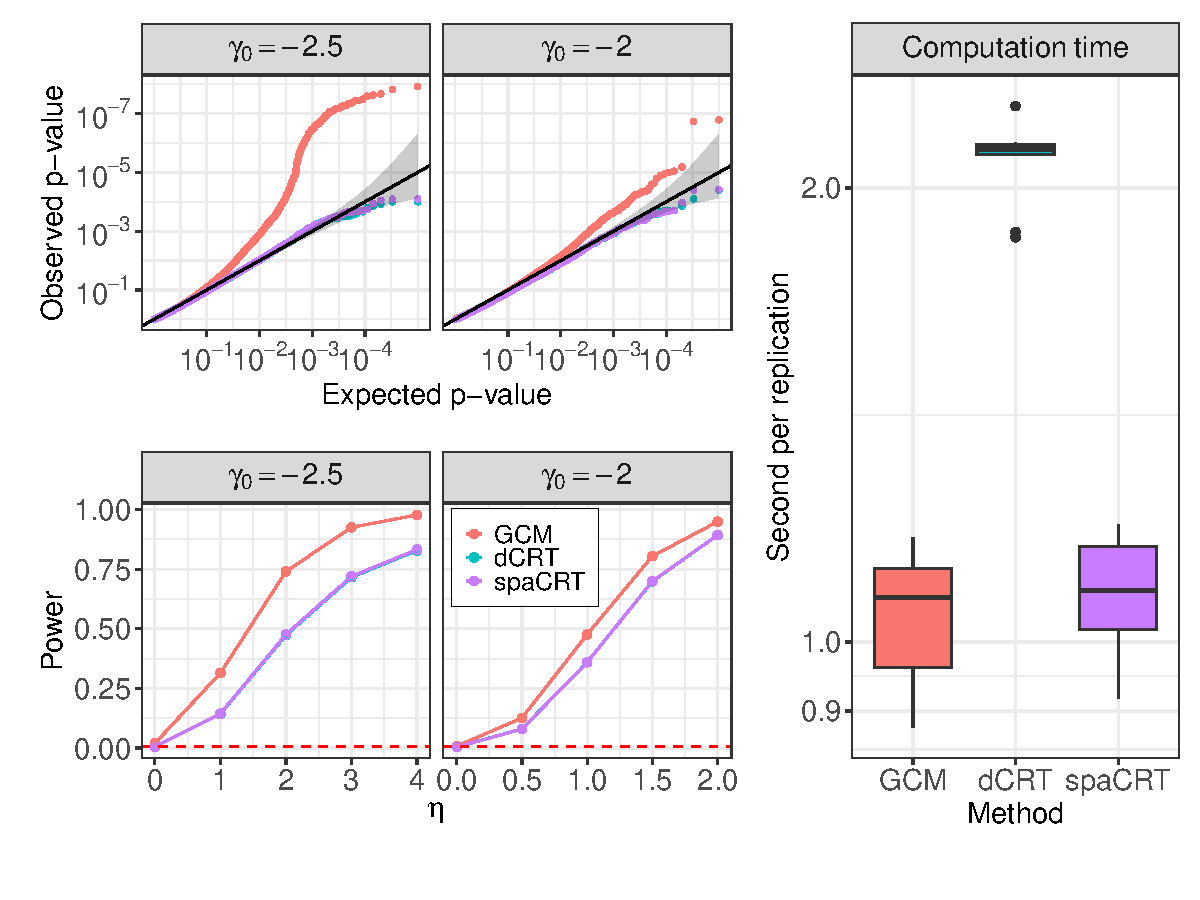
\includegraphics[width=1.0\textwidth]{figures-and-tables/simulation/RF-regression/simulation-summary.pdf}
  \caption{Summary of numerical simulation results for nonparametric regression. The simulation is repated $50000$ times.}
  \label{fig:simulation-summary-RF-classification}
\end{figure}

\section{Some useful lemmas and proofs}\label{sec:useful_lemma}

\subsection{Lemma statements}

\begin{lemma}[Lemma 3 in \cite{Niu2022a}]\label{lem:unified_asymptotic_equivalence}
	Consider two hypothesis tests based on the same test statistic $T_n(\srx, \sry, \srz)$ but different critical values:
	\begin{equation*}
		\phi_n^1(\srx, \sry, \srz) \equiv \indicator(T_n(\srx, \sry, \srz) > C_n(\srx, \sry, \srz)); \quad \phi_n^2(\srx, \sry, \srz) \equiv \indicator(T_n(\srx, \sry, \srz) > z_{1-\alpha}). 
	\end{equation*}
	If the critical value of the first converges in probability to that of the second:
	\begin{equation*}
		C_n(\srx, \sry, \srz) \convp z_{1-\alpha}
	\end{equation*}
	and the test statistic does not accumulate near the limiting critical value:
	\begin{equation}
		\lim_{\delta \rightarrow 0}\limsup_{n \rightarrow \infty}\ \P_{\law_n}[|T_n(\srx, \sry, \srz)-z_{1-\alpha}| \leq \delta] = 0,
		\label{eq:non-accumulation-app}
	\end{equation}
	then the two tests are asymptotically equivalent:
	\begin{equation*}
		\lim_{n \rightarrow \infty}\P_{\law_n}[\phi_n^{1}(\srx, \sry, \srz) = \phi_n^2(\srx, \sry, \srz)] = 1.
	\end{equation*}
\end{lemma}


\paragraph{\textbf{Regularity condition:}}
there exists $\delta>0$ such that for a sequence of laws $\law_n$ and its estimate $\lawhat_n$, the following assumptions hold:
\begin{align}
    (\widehat{S}_n^{\dCRT})^2=\frac{1}{n}\sum_{i=1}^n\V_{\lawhat_n}[\srx_{in}\mid \srz_{in}](\sry_{in}-\widehat{\mu}_{n,y}(\srz_{in}))^2=\Omega_\P(1) \label{eq:variance_lower_bound};\\
    \frac{1}{n^{1+\delta/2}} \sum_{i=1}^n |\sry_{in}-\widehat \mu_{n,y}(\srz_{in})|^{2+\delta}\E_{\lawhat_n}[|\srxk_{in}-\widehat\mu_{n,x}(\srz_{in})|^{2+\delta}\mid \srx,\srz] =o_\P(1)\label{eq:Lyapunov_condition_2};\\
    \V_{\lawhat_n}[\srx_{in}|\srz_{in}],(\sry_{in}-\widehat{\mu}_{n,y}(\srz_{in}))^2,(\sry_{in}-\mu_{n,y}(\srz_{in}))^2<\infty\ \text{almost surely}\label{eq:non_degeneracy}.
\end{align}

\begin{lemma}[Theorem 9 in \cite{Niu2022a}]\label{lem:quantile_convergence_ptwise}
	Let $\law_n$ be a sequence of laws and $\lawhat_n$ be a sequence of estimates. Suppose  there exists a sequence of laws $\law_n$ satisfying all the assumptions in \textbf{Regularity condition}. Then, the quantile of 
  \begin{align}\label{eq:normalized_dcrt_stats}
    T_n^{\ndCRThat}(\srxk,\srx,\sry,\srz)\equiv \frac{T_n^{\dCRT}(\srxk,\srx,\sry,\srz)}{\widehat S_n^{\dCRT}}
  \end{align}
  converges to the quantile of the standard normal distribution pointwisely in probability, i.e., for any $p\in(0,1)$,
	\begin{align*}
		\Q_{p}\left[n^{1/2}T_n^{\ndCRThat}(\srxk,\srx,\sry,\srz)|\srx,\sry,\srz\right]\convp z_{p}.
	\end{align*}
\end{lemma}

\begin{lemma}\label{lem:quantile_equivalence}
  Suppose the sequence of laws $\law_n$ and its estimate $\lawhat_n$ satisfy all the assumptions in Lemma~\ref{lem:quantile_convergence_ptwise}. Then for any given $\alpha\in (0,1)$, we have for any sequence $M_n\in\mathcal{F}_n$ satisfying $M_n=o_\P(1)$,
  \begin{align*}
  \Q_{1-\alpha(1+M_n)}\left[n^{1/2}T_n^{\ndCRThat}(\srxk, \srx, \sry,\srz)|\srx,\sry,\srz\right]\convp z_{1-\alpha}
  \end{align*}
  where $T_n^{\ndCRThat}(\srxk,\srx,\sry,\srz)$ is defined as in \eqref{eq:normalized_dcrt_stats}.
\end{lemma}

\begin{lemma}[Corollary 6 in \cite{Niu2022a}]\label{lem:wlln}
  Let $X_{in}$ be a triangular array of random variables, such that $X_{in}$ are independent for each $n$. If for some $\delta>0$ we have 
  \begin{align}\label{eq:moment_condition_wlln}
    \frac{1}{n^{1+\delta}}\sum_{i=1}^n \E[|X_{in}|^{1+\delta}]\rightarrow 0,
  \end{align}
  then 
  \begin{align*}
    \frac{1}{n}\sum_{i=1}^n (X_{in}-\E[X_{in}])\overset{\P}{\rightarrow}0.
  \end{align*}
  The condition \eqref{eq:moment_condition_wlln} is satisfied when 
  \begin{align*}
    \sup_{1\leq i\leq n}\E[|X_{in}|^{1+\delta}]=o(n^\delta).
  \end{align*}
\end{lemma}



\begin{lemma}[Conditional H\"older inequality, \cite{Swanson2019}, Theorem 6.60]\label{lem:cond_holder}
	Let $W_1$ and $W_2$ be random variables and let $\mathcal F$ be a $\sigma$-algebra. If for some $q_1, q_2 \in (1,\infty)$ with $\frac{1}{q_1} + \frac{1}{q_2} = 1$ we have $\E[|W_1|^{q_1}], \E[|W_2|^{q_2}] < \infty$, then
	\begin{align*}
		\E[|W_1 W_2| \mid \mathcal F] \leq (\E[|W_1|^{q_1} \mid \mathcal F])^{1/q_1}(\E[|W_2|^{q_2} \mid \mathcal F])^{1/q_2} \quad \text{almost surely}.
	\end{align*}
\end{lemma}

\begin{lemma}[Conditional Jensen inequality, \cite{Davidson2003}, Theorem 10.18] \label{lem:conditional-jensen}
	Let $W$ be a random variable and let $\phi$ be a convex function, such that $W$ and $\phi(W)$ are integrable. For any $\sigma$-algebra $\mathcal F$, we have the inequality
	\begin{equation*}
		\phi(\E[W \mid \mathcal F]) \leq  \E[\phi(W) \mid \mathcal F] \quad \text{almost surely}.
	\end{equation*}
\end{lemma}

\begin{lemma}[Conditional Markov's inequality, \cite{Davidson2003}, Theorem 10.17]\label{lem:conditional_Markov}
  Let $W$ be a random variable and let $\mathcal{F}$ be a $\sigma$-algebra. If for some $q>0$, we have $\E[|W|^q]<\infty$, then for any $\varepsilon$ we have
	\begin{equation*}
		\P[|W|\geq \varepsilon|\mathcal{F}]\leq \frac{\E[|W]^q}{\varepsilon^q}\quad\text{almost surely}.
	\end{equation*}
\end{lemma}

\begin{lemma}[Dominance of higher moment]\label{lem:moment_dominance}
  For any $1<p<q<\infty$, the following inequality is true almost surely:
  \begin{align*}
    \frac{1}{n}\sum_{i=1}^n \E[|X_{in}|^{p}|\mathcal{F}_n]\leq \left(\frac{1}{n}\sum_{i=1}^n \E[|X_{in}|^{q}|\mathcal{F}_n]\right)^{p/q}.
  \end{align*}
\end{lemma}


\begin{lemma}\label{lem:dCRT_convergence}
  Consider the fixed dimension setup: $(\srx_{in},\sry_{in},\srz_{in})=(\srx_{i},\sry_{i},\srz_{i})$ and $(\srz_{i},\srx_{i},\sry_{i})_{i\in[n]}$ are i.i.d. samples. Define $\sigma_{\dCRT}^2=\E[(\srx_i-\E[\srx_i|\srz_i])^2(\sry_i-\E[\sry_i|\srz_i])^2]$. Then if $\pry \mid \prz \sim f(\pry \mid \prz^\top \beta)$ for some natural exponential family $f$~\eqref{eq:NEF} with log-partition function $A_y$ and $\P[\|\srz_i\|_{\infty},\srx_i,\mu_x(\srz_i)\in [-S,S]]=1$ for some $S>0$, then as long as the following conditions hold:
  \begin{align*}
    \prx\indep\pry\mid \prz;\\
    \sigma_{\dCRT}^2\in (0,\infty);\\
    \frac{1}{n}\sum_{i=1}^n (\mu_{x}(\srz_i)-\widehat\mu_{x}(\srz_i))^2=o_{\P}(1);\\
    \frac{1}{n}\sum_{i=1}^n (\mu_{x}(\srz_i)-\widehat\mu_{x}(\srz_i))^2=o_{\P}(1);\\
    \left(\frac{1}{n}\sum_{i=1}^n (\mu_{x}(\srz_i)-\widehat\mu_{x}(\srz_i))^2\right)\left(
    \frac{1}{n}\sum_{i=1}^n (\mu_{x}(\srz_i)-\widehat\mu_{x}(\srz_i))^2\right)=o_{\P}(1/n),
  \end{align*}
  then we have $\sqrt{n}T_n^{\dCRT}\convp N(0,\sigma_{\dCRT}^2)$.
\end{lemma}

\begin{lemma}[Gaussian tail probability estimate]\label{lem:Gaussian_tail_estimate}
	For $x>0$, we have 
	\begin{align*}
		1-\Phi(x)-\frac{1}{\sqrt{2\pi}x}\exp(-x^2/2)
	  \left(1-\frac{1}{x^2}\right)=-\int_{x}^{\infty}\frac{\phi(t)}{3t^4}\mathrm{d}t.
	\end{align*}
	Consequently, we have 
	\begin{align*}
	  \left|1-\Phi(x)-\left(\frac{1}{\sqrt{2\pi}x}\exp(-x^2/2)
	  \left(1-\frac{1}{x^2}\right)\right)\right|\leq \frac{\phi(x)}{x^3}
	\end{align*}
	and 
	\begin{align*}
		\left|x\exp\left(\frac{x^2}{2}\right)(1-\Phi(x))-\frac{1}{\sqrt{2\pi}}\right|\leq \frac{2}{\sqrt{2\pi}}\frac{1}{x^2}.
	\end{align*}
\end{lemma}

\begin{lemma}[Lower bound on the Gaussian tail probability]\label{lem:lower_bound_Gaussian}
	For any $x\geq 0$, we have 
	\begin{align*}
	  1-\Phi(x)> \frac{1}{\sqrt{2\pi}}\frac{x}{x^2+1}\exp(-x^2/2).
	\end{align*}
\end{lemma}

\begin{lemma}\label{lem:existence_derivative_CGF}
	Consider the probability space $(\P,\Omega,\mathcal{F})$ and the $\sigma$-algebras $\mathcal{F}_n\subset \mathcal{F}$. Suppose the sequence of random variable $W_n$ satisfies there exists $\varepsilon>0$ such that 
	\begin{align*}
		\P\left[\E[|W_n|^p\exp(sW_n)|\mathcal{F}_n]<\infty,\ \forall s\in(-\varepsilon,\varepsilon),\ \forall n,p\in\mathbb{N}\right]=1
	\end{align*}
	Then defining $H_n(s)\equiv \E[\exp(sW_n)|\mathcal{F}_n]$, we have
	\begin{align*}
		\P\left[H_n(s) \text{ has }p\text{-th order derivative at the open neighborhood }(-\varepsilon,\varepsilon),\ \forall n,p\in\mathbb{N}\right]=1,
	\end{align*}
	and
	\begin{align*}
		\P\left[H_n^{(p)}(s)=\E[W_n^p\exp(sW_n)|\mathcal{F}_n],\forall s\in (-\varepsilon,\varepsilon),\ \forall n,p \in\mathbb{N}\right]=1.
	\end{align*}
\end{lemma}


\begin{lemma}[\cite{Chen2011}, Theorem 3.6]\label{lem:berry-esseen}
    Suppose $n\in\mathbb{N}$ and $\xi_{1n},\ldots,\xi_{nn}$ are independent random variables, satisfying for any $1\leq i\leq n$
    \begin{align*}
        \E[\xi_{in}]=0,\ \sum_{i=1}^n\E[\xi_{in}^2]=1.
    \end{align*}
	Then 
    \begin{align*}
        \sup_{t\in\mathbb{R}}\left|\P\left[\sum_{i=1}^n \xi_{in}\leq t\right]-\Phi(t)\right|\leq 9.4\sum_{i=1}^n \E[|\xi_{in}|^3].
    \end{align*}
\end{lemma}

  \begin{lemma}[Equivalence of the definition of CSE distribution]\label{lem:equivalence_CSE}
	  The following two statements are equivalent:
	  \begin{enumerate}
		  \item there exists positive parameters $(\lambda_{in},\gamma)$ with $\lambda_{in}\in\mathcal{F}_n$ and constant $\gamma$ such that 
		  \begin{align}\label{eq:cse_cgf}
			  \P\left[\mathcal{B}_1\right]=1,\ \mathcal{B}_1\equiv \left\{\E[\exp(sW_{in})|\mathcal{F}_n]\leq \exp(\lambda_{in}s^2),\ \forall s\in \left(-\frac{1}{\gamma},\frac{1}{\gamma}\right)\right\}.
		  \end{align}
		  \item there exists positive parameters $(\theta_{in},\beta)$ with $\theta_{in}\in\mathcal{F}_n$ and constant $\beta$ such that 
		  \begin{align}\label{eq:cse_tail}
			  \P\left[\mathcal{B}_2\right]=1,\ \mathcal{B}_2\equiv  \left\{\P\left[|W_{in}|\geq t|\mathcal{F}_n\right]\leq \theta_{in}\exp(-\beta t),\ \forall t>0\right\}.
		  \end{align}
	  \end{enumerate}
	  In particular, the suppose condition \eqref{eq:cse_tail} holds, then we can choose $(\lambda_{in},\gamma)$ in \eqref{eq:cse_cgf} as
	  \begin{align*}
		  \lambda_{in}= \frac{\sqrt{6!4^6}(1+\theta_{in})}{24\beta^2}+\frac{16(1+\theta_{in})}{\beta^2},\ \gamma=\frac{4}{\beta}.
	  \end{align*}
  \end{lemma}


\subsection{Proof of Lemma \ref{lem:quantile_equivalence}}
  
\begin{proof}[Proof of Lemma \ref{lem:quantile_equivalence}]
  For any given $\varepsilon\in (0,\min\{1/\alpha-1,1\}),\eta>0$, there exists $N(\varepsilon,\eta)$ such that 
  \begin{align*}
    \P[|M_n|>\varepsilon]<\eta,\ \forall n\geq N(\varepsilon,\eta).
  \end{align*}
  This is true because $M_n=o_\P(1)$. We will use $T_n^{\ndCRThat}$ to denote $T_n^{\ndCRThat}(\srxk,\srx,\sry,\srz)$. Then consider the $1-\alpha(1-\varepsilon)$ and $1-\alpha(1+\varepsilon)$ conditional quantiles of $T_n^{\ndCRThat}$. We have with probability at least $1-\eta$, for large enough $n$, the following is true:
  \begin{align*}
    \Q_{1-\alpha(1-\varepsilon)}\left[T_n^{\ndCRThat}|\srx,\sry,\srz\right]\geq \Q_{1-\alpha(1+M_n)}\left[T_n^{\ndCRThat}|\srx,\sry,\srz\right]\geq \Q_{1-\alpha(1+\varepsilon)}\left[T_n^{\ndCRThat}|\srx,\sry,\srz\right].
  \end{align*}
  Then with probability at least $1-\eta$, for sufficiently large $n$, we have
  \begin{align}\label{eq:quantile_upper_bound}
    |\Q_{1-\alpha(1+M_n)}\left[T_n^{\ndCRThat}|\srx,\sry,\srz\right] - z_{1-\alpha}|\leq A_n + B_n
  \end{align}
  where 
  \begin{align*}
    A_n\equiv \left|\Q_{1-\alpha(1-\varepsilon)}\left[T_n^{\ndCRThat}|\srx,\sry,\srz\right]- z_{1-\alpha}\right|,\ B_n\equiv \left|\Q_{1-\alpha(1+\varepsilon)}\left[T_n^{\ndCRThat}|\srx,\sry,\srz\right]- z_{1-\alpha}\right|.
  \end{align*}
  Applying Lemma \ref{lem:quantile_convergence_ptwise}, we have 
  \begin{align*}
    \Q_{1-\alpha(1-\varepsilon)}\left[T_n^{\ndCRThat}|\srx,\sry,\srz\right]\convp z_{1-\alpha(1-\varepsilon)},\ \Q_{1-\alpha(1+\varepsilon)}\left[T_n^{\ndCRThat}|\srx,\sry,\srz\right]\convp z_{1-\alpha(1+\varepsilon)}.
  \end{align*}
  Thus for the given $\varepsilon$ and sufficiently large $n$, we have with probability at least $1-\eta$,
  \begin{align*}
    A_n< \varepsilon+|z_{1-\alpha(1-\varepsilon)}-z_{1-\alpha}|,\ B_n< \varepsilon+|z_{1-\alpha(1+\varepsilon)}-z_{1-\alpha}|.
  \end{align*}
  By the continuity of the quantile function of standard normal distribution, we know there exists a universal constant $C_\alpha$ that only depends on $\alpha$ such that 
  \begin{align*}
    |z_{1-\alpha(1+\varepsilon)}-z_{1-\alpha}| < C_\alpha\varepsilon,\ |z_{1-\alpha(1-\varepsilon)}-z_{1-\alpha}|< C_\alpha\varepsilon.
  \end{align*}
  Then combining \eqref{eq:quantile_upper_bound}, we know with probability at least $1-2\eta$, for sufficiently large $n$, we have 
  \begin{align*}
    \left|\Q_{1-\alpha(1+M_n)}\left[T_n^{\ndCRThat}|\srx,\sry,\srz\right] - z_{1-\alpha}\right|\leq A_n+B_n< 2C_\alpha\varepsilon + 2\varepsilon.
  \end{align*}
  Then since $\eta,\varepsilon$ is arbitrary, we have
  \begin{align*}
  \Q_{1-\alpha(1+M_n)}\left[T_n^{\ndCRThat}|\srx,\sry,\srz\right]\convp z_{1-\alpha}.
  \end{align*}
  Therefore we complete the proof.
\end{proof}

\subsection{Proof of Lemma \ref{lem:moment_dominance}}

\begin{proof}[Proof of Lemma \ref{lem:moment_dominance}]
  By Lemma \ref{lem:cond_holder}, we have
  \begin{align*}
    \frac{1}{n}\sum_{i=1}^n \E[|X_{in}|^{p}|\mathcal{F}_n]
    &
    \leq 
    \frac{1}{n}\left(\sum_{i=1}^n \left(\E[|X_{in}|^{p}|\mathcal{F}_n]\right)^{q/p}\right)^{p/q}n^{1-p/q}\\
    &
    =\left(\frac{1}{n}\sum_{i=1}^n \left(\E[|X_{in}|^{p}|\mathcal{F}_n]\right)^{q/p}\right)^{p/q}.
  \end{align*}
  We use Jensen's inequality, Lemma \ref{lem:conditional-jensen}, to obtain
  \begin{align*}
    \frac{1}{n}\sum_{i=1}^n \E[|X_{in}|^{p}|\mathcal{F}_n]\leq \left(\frac{1}{n}\sum_{i=1}^n \E[|X_{in}|^{q}|\mathcal{F}_n]\right)^{p/q}.
  \end{align*}
\end{proof}

\subsection{Proof of Lemma \ref{lem:dCRT_convergence}}
\begin{proof}[Proof of Lemma~\ref{lem:dCRT_convergence}]
	
We consider the following decomposition:
\begin{align*}
  T_n^{\dCRT}
  &
  =\frac{1}{n}\sum_{i=1}^n (\srx_i-\mu_x(\srz_i))(\sry_i-\mu_y(\srz_i)) + \frac{1}{n}\sum_{i=1}^n (\mu_{x}(\srz_i)-\widehat{\mu}_{x}(\srz_i))(\sry_i-\mu_{y}(\srz_i))\\
  &
  + \frac{1}{n}\sum_{i=1}^n (\srx_i-\mu_{x}(\srz_i))(\mu_{y}(\srz_i)-\widehat{\mu}_{y}(\srz_i))+\frac{1}{n}\sum_{i=1}^n (\mu_{x}(\srz_i)-\widehat{\mu}_{x}(\srz_i))(\mu_{y}(\srz_i)-\widehat{\mu}_{y}(\srz_i))\\
  &
  \equiv \frac{1}{n}\sum_{i=1}^n (\srx_i-\mu_x(\srz_i))(\sry_i-\mu_y(\srz_i))+\sum_{k=1}^3B_k.
\end{align*}
We will prove $\sqrt{n}B_k$ converges $0$ in probability for any $k=1,2,3$. First, by the assumption $\sry_i\sim f( \cdot \mid \srz_i^\top\beta)$ for NEF $f$ with log-partition function $A_y$ and H\"older's inequality $|\srz_i^\top\beta|\leq \|\srz_i\|_{\infty}\|\beta\|_1\leq S\|\beta\|_1$, we have, almost surely,
\begin{align*}
	\E[(\sry_i-\mu_{y}(\srz_i))^2|\srz]=A_y''(\srz_i^\top\beta)\leq \sup_{t\in [-S\|\beta\|_1,S\|\beta\|_1]}A''(t)<\infty.
\end{align*}
Therefore, for $B_1$, we have 
\begin{align*}
  \P\left[\sqrt{n}B_1>\varepsilon|\srx,\srz\right]\leq \frac{1}{\varepsilon^2n}\sum_{i=1}^n (\mu_{x}(\srz_i)-\widehat{\mu}_{x}(\srz_i))^2\E[(\sry_i-\mu_{y}(\srz_i))^2|\srz]=o_{\P}(1).
\end{align*}
For $B_2$, by the assumption that $\P[X_i,\mu_x(\srz_i)\in [-S,S]]=1$, we have
\begin{align*}
  \P\left[\sqrt{n}B_2>\varepsilon|\srx,\srz\right]\leq \frac{1}{\varepsilon^2n}\sum_{i=1}^n (\mu_{y}(\srz_i)-\widehat{\mu}_{y}(\srz_i))^2\E[(\srx_i-\mu_{x}(\srz_i))^2|\srz]=o_{\P}(1).
\end{align*}
As for $B_3$, we know by Cauchy-Schwarz inequality that
\begin{align*}
  \sqrt{n}|B_3|\leq \sqrt{n}\sqrt{\frac{1}{n}\sum_{i=1}^n (\mu_{x}(\srz_i)-\widehat{\mu}_{x}(\srz_i))^2}\sqrt{\frac{1}{n}\sum_{i=1}^n (\mu_{y}(\srz_i)-\widehat{\mu}_{y}(\srz_i))^2}=o_{\P}(1).
\end{align*}
Therefore, we only need to prove the weak convergence of $\sum_{i=1}^n (\srx_i-\mu_x(\srz_i))(\sry_i-\mu_y(\srz_i))/\sqrt{n}$. This is true by classical CLT, guaranteed by the assumption that $\sigma_{\dCRT}\in(0,\infty)$.
\end{proof}


\subsection{Proof of the Lemma \ref{lem:Gaussian_tail_estimate}}

  \begin{proof}[Proof of Lemma \ref{lem:Gaussian_tail_estimate}]
    Applying integration by parts, we can write 
    \begin{align*}
      1-\Phi(x)
      &
      =\int_{x}^{\infty}\phi(t)\mathrm{d}t\\
      &
      =\int_{x}^{\infty}\frac{1}{t}\frac{t}{\sqrt{2\pi}}\exp(-t^2/2)\mathrm{d}t\\
      &
      =-\frac{1}{t}\frac{1}{\sqrt{2\pi}}\exp(-t^2/2)\bigg|_{x}^{\infty}-\int_{x}^{\infty}\frac{\phi(t)}{t^2}\mathrm{d}t\\
      &
      =\frac{\phi(x)}{x}+\frac{1}{t^3}\frac{1}{\sqrt{2\pi}}\exp(-t^2/2)\bigg|_x^{\infty}-\int_x^{\infty}\frac{\phi(t)}{3t^4}\mathrm{d}t\\
      &
      =\frac{\phi(x)}{x}-\frac{\phi(x)}{x^3}-\int_x^{\infty}\frac{\phi(t)}{3t^4}\mathrm{d}t.
    \end{align*}
    Then we can bound for $x>0$
    \begin{align*}
      \left|\int_{x}^{\infty}\frac{\phi(t)}{3t^4}\mathrm{d}t\right|\leq \phi(x)\int_{x}^{\infty}\frac{1}{3t^4}\mathrm{d}t\leq \frac{\phi(x)}{x^3}.
    \end{align*}
  \end{proof}


    
\subsection{Proof of Lemma \ref{lem:lower_bound_Gaussian}}

\begin{proof}[Proof of Lemma \ref{lem:lower_bound_Gaussian}]
  Define 
  \begin{align*}
	g(x)\equiv 1-\Phi(x)-\frac{1}{\sqrt{2\pi}}\frac{x}{x^2+1}\exp(-x^2/2).
  \end{align*}
  Computing the derivative we obtain 
  \begin{align*}
	g'(x)=-\frac{2}{\sqrt{2\pi}}\frac{e^{-x^2/2}}{(x^2+1)^2}<0.
  \end{align*}
  Also notice $g(0)=1/2>0$ and $\lim_{x\rightarrow\infty}g(x)=0$. This completes the proof.
\end{proof}

\subsection{Proof of Lemma \ref{lem:existence_derivative_CGF}}

\begin{proof}[Proof of Lemma \ref{lem:existence_derivative_CGF}]
	Consider the regular conditional distribution $W_n|\mathcal{F}_n$ to be $\kappa_{W_n}$. We use induction to prove the existence of the $p$-th derivative of $H_n(s)$. Suppose 
	\begin{align}\label{eq:induction_derivative}
		\P\left[H_n^{(p)}(s)=\E[W_n^p\exp(sW_n)|\mathcal{F}_n],\ \forall s\in (-\varepsilon,\varepsilon)\right]=1
	\end{align} 
	and 
	\begin{align}\label{eq:induction_assumption}
		\P\left[\E[|W_n|^{p+1}\exp(sW_n)|\mathcal{F}_n]<\infty,\ \forall s\in(-\varepsilon,\varepsilon)\right]=1.
	\end{align}
	According to the definition of derivative, we write 
	\begin{align}\label{eq:derivative_definition}
		H_n^{(p+1)}(s)\equiv \lim_{h\rightarrow0}\frac{H_n^{(p)}(s+h)-H_n^{(p)}(s)}{h}.
	\end{align} 
	Then on the event in hypothesis \eqref{eq:induction_derivative}, we have for any $s\in (-\varepsilon,\varepsilon)$
	\begin{align*}
		H_n^{(p)}(s)=\E[W_n^p\exp(sW_n)|\mathcal{F}_n]=\int x^p\exp(sx)\mathrm{d}\kappa_{W_n}(\cdot,x).
	\end{align*}
	Fix any $s_0\in (-\varepsilon,\varepsilon)$ and find $r_0\in (s_0,\varepsilon)$ such that $|r_0|>|s_0|$. We find small enough $h$ such that $|h|<\min\{|r_0|-s_0,|r_0|+s_0\}$. Thus we have
	\begin{align}\label{eq:interval_s_plus_h}
		-\varepsilon <-|r_0|=s_0-|r_0|-s_0<s_0+h< s_0+|r_0|-s_0 = |r_0|<\varepsilon.
	\end{align} 
	Also we notice, $|s_0|<|r_0|$ so that $s_0x\in (-|r_0x|,|r_0x|)$. Also, the derivation in \eqref{eq:interval_s_plus_h} informs $(s_0+h)x$ belong to the interval $(-|r_0x|,|r_0x|)$. Therefore, both $s_0x$ and $(s_0+h)x$ belong to $(-|r_0x|,|r_0x|)$. Then we have
	\begin{align}
		|\exp((s_0+h)x)-\exp(s_0x)|
		&\nonumber
		=\left|\int_{s_0x}^{(s_0+h)x}e^{y}\mathrm{d}y\right|\\
		&\nonumber
		\leq |hx|\sup_{y\in [-|r_0x|,|r_0x|]}\exp(y)\\
		&\label{eq:finite_diff_bound}
		\leq |hx|\{\exp(r_0 x)+\exp(-r_0 x)\}.
	\end{align}
	By the definition \eqref{eq:derivative_definition}, we have
	\begin{align*}
		H^{(p+1)}_n(s_0)
		&
		=\lim_{h\rightarrow 0}\E\left[W_n^p \frac{\exp((s_0+h)W_n)-\exp(s_0W_n)}{h}|\mathcal{F}_n\right]\\
		&
		=\lim_{h\rightarrow 0}\int x^p\frac{\exp((s_0+h)x)-\exp(s_0x)}{h}\mathrm{d}\kappa_{W_n}(\cdot,x).
	\end{align*}
	Then by \eqref{eq:finite_diff_bound}, we can bound 
	\begin{align*}
		\left|x^p \frac{\exp((s_0+h)x)-\exp(s_0x)}{h}\right|\leq |x|^{p+1}\exp(r_0 x)+|x|^{p+1}\exp(-r_0 x).
	\end{align*}
	Notice the RHS is independent of $h$ and integrable with respect to measure $\kappa_{W_n}(\omega,\cdot)$ for almost every $\omega\in\Omega$, by the induction hypothesis \eqref{eq:induction_assumption} since $r_0\in(-\varepsilon,\varepsilon)$. By dominated convergence theorem, we know on the event in hypothesis \eqref{eq:induction_assumption},
	\begin{align*}
		H^{(p+1)}_n(s_0)
		&
		=\int \lim_{h\rightarrow0}x^p\frac{\exp((s_0+h)x)-\exp(s_0x)}{h}\mathrm{d}\kappa_{W_n}(\cdot,x)\\
		&
		=\int x^{p+1}\exp(s_0x)\mathrm{d}\kappa_{W_n}(\cdot,x)\\
		&
		=\E[ W_n^{p+1}\exp(s_0W_n)|\mathcal{F}_n].
	\end{align*}
	Then, by the arbitrary choice of $s_0\in (-\varepsilon,\varepsilon)$, we know on the event in hypothesis \eqref{eq:induction_assumption}, $H^{(p+1)}(s)$ is well-defined on the interval $(-\varepsilon,\varepsilon)$ and takes the form 
	\begin{align*}
		H^{(p+1)}(s)=\E[ W_n^{p+1}\exp(s_0W_n)|\mathcal{F}_n].
	\end{align*}
	Thus we have proved for the case $p+1$ so that we complete the induction and conclude the proof.
\end{proof}

\subsection{Proof of Lemma \ref{lem:equivalence_CSE}}

\begin{proof}[Proof of Lemma \ref{lem:equivalence_CSE}]
	We prove two directions separately. 
	\paragraph{\eqref{eq:cse_cgf}$\Rightarrow $\eqref{eq:cse_tail}:}
	For any $\omega\in \mathcal{B}_1$, we know by definition \eqref{eq:def_conditional_expectation} that
	\begin{align*}
		\E[\exp(sW_{in})|\mathcal{F}_n](\omega)=\int \exp(sx)\mathrm{d}\kappa_{in}(\omega,x)<\infty,\ \forall s\in \left(-\frac{1}{\gamma},\frac{1}{\gamma}\right).
	\end{align*}
	Then the Chernoff bound gives 
	\begin{align*}
		\int \indicator(x\geq t)\mathrm{d}\kappa_{in}(\omega,x)\leq \int \exp\left(\frac{x}{2\gamma}\right)\mathrm{d}\kappa_{in}(\omega,x)\exp\left(-\frac{t}{2\gamma}\right).
	\end{align*}
	Applying a similar argument to $\indicator(-x\geq t)$, we conclude 
	\begin{align*}
		\int \indicator(|x|\geq t)\mathrm{d}\kappa_{in}(\omega,x)\leq \left(\int \exp\left(\frac{x}{2\gamma}\right)+\exp\left(\frac{-x}{2\gamma}\right)\mathrm{d}\kappa_{in}(\omega,x)\right)\cdot \exp\left(-\frac{t}{2\gamma}\right).
	\end{align*}
	Thus we know 
	\begin{align*}
		\P\left[|W_{in}|\geq t|\mathcal{F}_n\right]
		&
		=\int\indicator(|x|\geq t)\mathrm{d}\kappa_{in}(\omega,x)\\
		&
		\leq \left(\E\left[\exp(W_{in}/(2\gamma))|\mathcal{F}_n\right]+\E\left[\exp(-W_{in}/(2\gamma))|\mathcal{F}_n\right]\right)\cdot \exp(-t/(2\gamma)).
	\end{align*}
	Thus $\P[\mathcal{B}_2]=1$ with
	\begin{align*}
		\theta_{in}=\E\left[\exp(W_{in}/(2\gamma))|\mathcal{F}_n\right]+\E\left[\exp(-W_{in}/(2\gamma))|\mathcal{F}_n\right],\ \beta=\frac{1}{2\gamma}.
	\end{align*}

	\paragraph{\eqref{eq:cse_tail}$\Rightarrow$\eqref{eq:cse_cgf}:}

	Fix a constant $a>0$ and $T>0$. For any $\omega\in \mathcal{B}_2$, we have 
	\begin{align*}
		&
		\E\left[\exp(a|W_{in}|)\indicator(\exp(a|W_{in}|)\leq \exp(aT))|\mathcal{F}_n\right](\omega)\\
		&
		=\int \exp(a|x|)\indicator(\exp(a|x|)\leq \exp(aT))\mathrm{d}\kappa_{in}(\omega,x)\\
		&
		\leq \int \min \{\exp(a|x|),\exp(aT)\}\mathrm{d}\kappa_{in}(\omega,x)\\
		&
		=\int \int_0^{e^{aT}}\indicator(\exp(a|x|)\geq t)\mathrm{d}t\mathrm{d}\kappa_{in}(\omega,x)\\
		&
		=\int_0^{e^{aT}}\int \indicator(\exp(a|x|)\geq t)\mathrm{d}\kappa_{in}(\omega,x)\mathrm{d}t\\
		&
		\leq 1+ \int_1^{e^{aT}}\int \indicator(|x|\geq \log(t)/a)\mathrm{d}\kappa_{in}(\omega,x)\mathrm{d}t
	\end{align*}
	where the last equality is due to Fubini's theorem. Then by the definition of $\mathcal{B}_2$, we obtain 
	\begin{align*}
		\E\left[\exp(a|W_{in}|)\indicator(\exp(a|W_{in}|)\leq \exp(aT))|\mathcal{F}_n\right](\omega)
		&
		\leq 1+\theta_{in}(\omega)\int_1^{e^{aT}}e^{-(\beta\log(t))/a}\mathrm{d}t\\
		&
		=1+\theta_{in}(\omega)\int_{1}^{e^{aT}}t^{-\beta/a}\mathrm{d}t.
	\end{align*}
	For $a\in [0,\beta/2]$, we have 
	\begin{align*}
		\E\left[\exp(a|W_{in}|)\indicator(\exp(a|W_{in}|)\leq \exp(aT))|\mathcal{F}_n\right](\omega)
		&
		=1+\theta_{in}(\omega)\frac{1}{1-\beta/a}t^{1-\beta/a}\bigg|_{1}^{e^{aT}}\\
		&
		\leq 1+\theta_{in}(\omega)\frac{1}{\beta/a - 1}(1-e^{(aT-\beta T)})\\
		&
		\leq 1+\theta_{in}(\omega).
	\end{align*}
	Then by Fatou's lemma, we have for any $a\in [0,\beta/2]$,
	\begin{align}
		\E\left[\exp(a|W_{in}|)|\mathcal{F}_n\right](\omega)
		&\nonumber
		=\int \exp(a|x|)\mathrm{d}\kappa_{in}(\omega,x)\\
		&\label{eq:upper_bound_cgf}
		\leq \liminf_{T\rightarrow\infty}\int \exp(a|x|)\indicator(e^{a|x|}\leq e^{aT})\mathrm{d}\kappa_{in}(\omega,x)\leq 1+\theta_{in}(\omega).
	\end{align}
	Then by Taylor's expansion, for any $|s|\leq \beta/4$
	\begin{align*}
		\E[\exp(sW_{in})|\mathcal{F}_n](\omega)
		&
		=\int \exp(sx)\mathrm{d}\kappa_{in}(\omega,x)\\
		&
		=\int 1+sx+\frac{s^2x^2}{2}+\frac{s^3x^3}{6}\exp(y(x))\mathrm{d}\kappa_{in}(\omega,x),\ |y(x)|\leq  |sx|.
	\end{align*}
	Then the assumption $\E[W_{in}|\mathcal{F}_n]=0$ implies for $|s|\leq \beta/4$,
	\begin{align}
		\E[\exp(sW_{in})|\mathcal{F}_n](\omega)
		&\nonumber
		\leq 1+\frac{s^2\E[W_{in}^2|\mathcal{F}_n](\omega)}{2}+\frac{s^2\beta}{24}\int |x|^3\exp(y(x))\mathrm{d}\kappa_{in}(\omega,x)\\
		&\nonumber
		\leq 1+\frac{s^2\E[W_{in}^2|\mathcal{F}_n](\omega)}{2}+\frac{s^2\beta}{24}\int |x|^3\exp(|sx|)\mathrm{d}\kappa_{in}(\omega,x)\\
		&\nonumber
		\leq 1+\frac{s^2\E[W_{in}^2|\mathcal{F}_n](\omega)}{2}+\frac{s^2\beta}{24}\sqrt{\E[W_{in}^6|\mathcal{F}_n](\omega)\E[\exp(2|sW_{in}|)|\mathcal{F}_n](\omega)}\\
		&\nonumber
		\leq 1+\left(\frac{\beta \sqrt{1+\theta_{in}(\omega)}\sqrt{\E[W_{in}^6|\mathcal{F}_n](\omega)}}{12}+\E[W_{in}^2|\mathcal{F}_n](\omega)\right)\frac{s^2}{2}\\
		&\label{eq:cse_bound}
		\leq \exp\left(\left(\frac{\beta \sqrt{1+\theta_{in}(\omega)}\sqrt{\E[W_{in}^6|\mathcal{F}_n](\omega)}}{12}+\E[W_{in}^2|\mathcal{F}_n](\omega)\right)\frac{s^2}{2}\right).
	\end{align}
	where the second inequality is due to $|y(x)|\leq|sx|$, the third inequality is due to Cauchy-Schwarz inequality, the fourth inequality is due to conclusion \eqref{eq:upper_bound_cgf} and the last inequality is due to the inequality $\exp(x)\geq 1+x$ for any $x\in\mathbb{R}$. Now by Fubini's theorem and conclusion \eqref{eq:upper_bound_cgf}, we have 
	\begin{align*}
		1+\theta_{in}(w)\geq \E[\exp(s|W_{in}|)|\mathcal{F}_n]=1+\sum_{k=1}^{\infty}\frac{s^k}{k!}\E[|W_{in}|^k|\mathcal{F}_n],\ \forall s\in [0,\beta/2].
	\end{align*}
	Then by setting $s=\beta/4$, we have
	\begin{align*}
		\E[W_{in}^2|\mathcal{F}_n]
		&
		\leq \frac{2!4^2}{\beta^2}\E[\exp(\beta|W_{in}|/4)|\mathcal{F}_n]\leq \frac{2!4^2}{\beta^2}(1+\theta_{in}),\\
		\E[W_{in}^6|\mathcal{F}_n]
		&
		\leq \frac{6!4^6}{\beta^6}\E[\exp(\beta|W_{in}|/4)|\mathcal{F}_n]\leq \frac{6!4^6}{\beta^6}(1+\theta_{in})
	\end{align*}
	Then choosing 
	\begin{align*}
		\lambda_{in}= \frac{\sqrt{6!4^6}(1+\theta_{in})}{24\beta^2}+\frac{16(1+\theta_{in})}{\beta^2}\geq \frac{\beta\sqrt{1+\theta_{in}}\sqrt{\E[W_{in}^6|\mathcal{F}_n]}}{24} +\frac{\E[W_{in}^2|\mathcal{F}_n]}{2},\ \gamma=\frac{4}{\beta},
	\end{align*}
	so that by bound \eqref{eq:cse_bound}, we obtain
	\begin{align*}
		\E[\exp(sW_{in})|\mathcal{F}_n](\omega)\leq \exp(\lambda_{in}(\omega)s^2),\ \forall s\in \left(-\frac{1}{\gamma},\frac{1}{\gamma}\right).
	\end{align*}
\end{proof}

\section{Proof of Theorem~\ref{thm:unified_unnormalized_moment_conditions}} \label{sec:spa_proof}

The high-level structure of our proof is inspired by that of \citet{Robinson1982}: Exponentially tilt the summands, then apply the Berry-Esseen inequality to get a normal approximation after tilting, then tilt back. In this section, we sketch the proof our main result with the help of a sequence of lemmas, whose proofs we defer to Appendix~\ref{sec:lemma_proofs}. 

\subsection{Solving the saddlepoint equation}\label{sec:solution_spa}

First, we state a lemma lower-bounding the second derivative $K''_n(s)$, which will help us guarantee the existence and uniqueness of solutions to the saddlepoint equation~\eqref{eq:saddlepoint-equation}.
\begin{lemma} \label{lem:positive_second_derivative}
Under the assumptions in Theorem \ref{thm:unified_unnormalized_moment_conditions}, the function $K''_n(s)$ is nonnegative on $(-\varepsilon, \varepsilon)$:
\begin{align}
K''_n(s) \geq 0 \quad \text{for all } s \in (-\varepsilon, \varepsilon) \text{ almost surely}. \label{eq:positive_second_derivative}
\end{align}
Furthermore, it is uniformly bounded away from zero on a neighborhood of the origin, in the sense that for each $\delta > 0$, there exist $\eta > 0, s^* \in (0, \varepsilon/2)$ and $N \in \mathbb N_+$ such that 
\begin{equation}
\P\left[\inf_{s \in [-s_*, s_*]} K''_n(s) \geq \eta\right] \geq 1-\delta \quad \text{for all } n \geq N. \label{eq:uniform_lower_bound_second_derivative}
\end{equation}
\end{lemma}
\noindent This lemma guarantees that the function $K'_n(s)$ is nondecreasing on $(-\varepsilon, \varepsilon)$ and increasing at a positive rate near the origin. To better illustrate the intuition, we refer the reader to Figure \ref{fig:illustration_spsolution}. Since $w_n \convp 0$, this implies that the saddlepoint equation~\eqref{eq:saddlepoint-equation} will have a solution for large enough $n$. 

\begin{figure}[!ht]
	\centering
	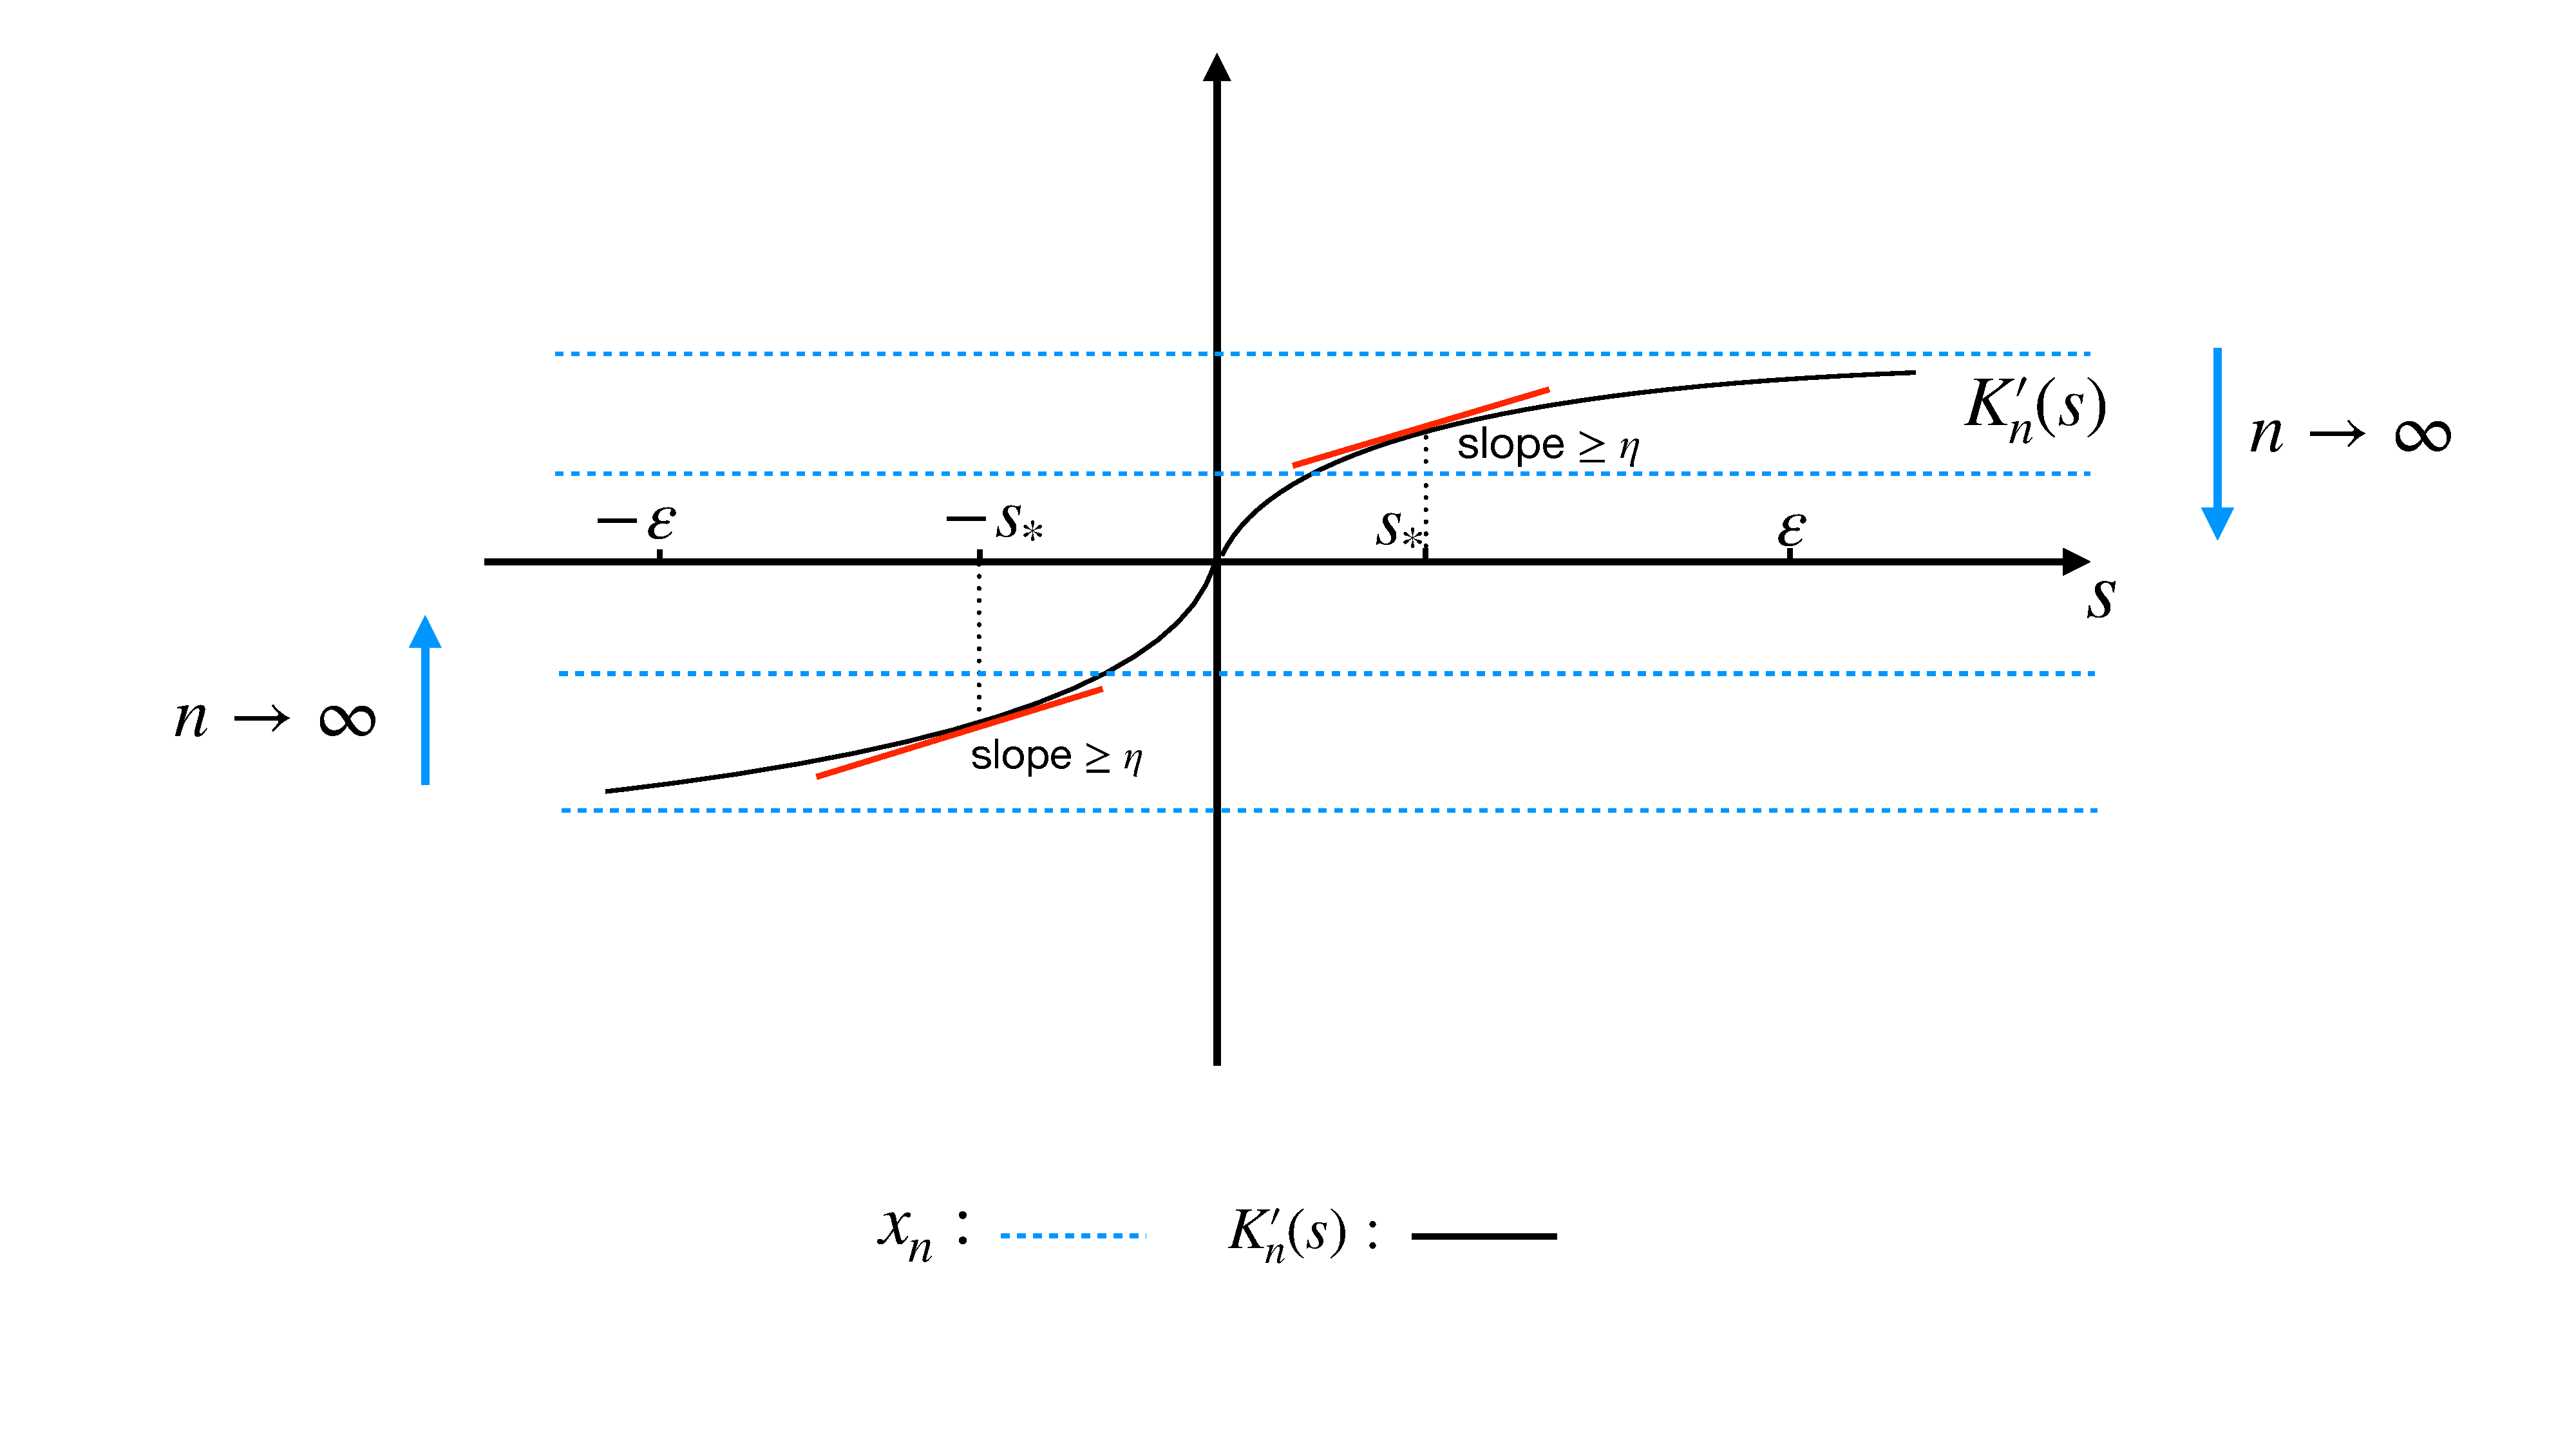
\includegraphics[width=1\textwidth]{figures-and-tables/illustration_spsolution.pdf}
	\caption{Illustration of the function $K'_n(s)$ for $n$ large. The derivative of the function is nonnegative and strictly positive near the origin.}
	\label{fig:illustration_spsolution}
\end{figure}

To be more precise, fix $\delta > 0$. By Lemma~\ref{lem:positive_second_derivative} and the fact that $w_n \convp 0$, let $\eta > 0$, $s_* \in (0, \varepsilon/2)$ and $N \in \mathbb N_+$ be such that
\begin{equation}
\P\left[\mathcal E_n\right] \geq 1-\delta \quad \text{for all } n \geq N, \quad \text{where} \quad \mathcal E_n \equiv \left\{\inf_{s \in [-s_*, s_*]} K''_n(s) \geq \eta, |w_n| < s_* \eta\right\}.
\end{equation}
On the event $\mathcal E_n \cap \mathcal A$, we can Taylor expand $K'_n(s)$ around $s = 0$ to obtain
\begin{equation}
K'_n(s) =  K'_n(0) + s K''_n(\bar s) = s K''_n(\bar s) \quad \text{for} \quad |\bar s| \in (0, |s|),
\label{eq:K_prime_taylor_expansion}
\end{equation}
where we have used the fact that
\begin{equation}
K'_n(0) = \frac{1}{n}\sum_{i = 1}^n K'_{in}(0) = \frac{1}{n}\sum_{i = 1}^n \E[W_{in} \mid \mathcal F_n] = 0. 
\label{eq:k_n_prime_0_equals_0}
\end{equation}
It follows from the Taylor expansion~\eqref{eq:K_prime_taylor_expansion} that, for $n \geq N$, we have
\begin{equation*}
K'_n(-s_*) \leq -s_* \eta < w_n < s_* \eta \leq K'_n(s_*).
\end{equation*}
By the continuity of $K'_n(s)$ on the event $\mathcal A$ (Lemma~\ref{lem:finite_cgf}), the intermediate value theorem implies that for each $n \geq N$, there exists a solution $\hat s_n \in (-s_*, s_*)$ to the saddlepoint equation~\eqref{eq:saddlepoint-equation} on the event $\mathcal E_n \cap \mathcal A$. Furthermore, for each $n \geq N$, this solution is unique on $\mathcal E_n \cap \mathcal A$ because $K'_n(s)$ is strictly increasing on $[-s_*, s_*]$ and nondecreasing on the entire interval $[-\varepsilon/2, \varepsilon/2]$. Hence, we have shown that, for arbitrary $\delta > 0$, we have
\begin{equation}
\liminf_{n \rightarrow \infty} \P[|S_n| = 1] \geq \liminf_{n \rightarrow \infty} \P[\mathcal E_n \cap \mathcal A] \geq 1 - \delta.
\end{equation}
Letting $\delta \rightarrow 0$ implies the first claim~\eqref{eq:unique_solution_in_probability} of Theorem~\ref{thm:unified_unnormalized_moment_conditions}. 

The following lemma records three properties of the saddlepoint $\hat s_n$, which will be useful in the remainder of the proof:
\begin{lemma} \label{lem:saddlepoint_properties}
The saddlepoint $\hat s_n$ satisfies the following properties:
\begin{align}
\sgn(\hat s_n)=\sgn(w_n)\ \text{almost surely} ;\label{eq:sign_property_s_n}  \\
\hat s_n \convp 0; \label{eq:hat_s_n_convergence} \\
K''_n(\hat s_n) = \Omega_{\P}(1). \label{eq:hat_s_n_second_derivative}
\end{align}
\end{lemma}

\subsection{Decomposing based on the sign of $w_n$}\label{sec:sign_decomposition}

Since $w_n$ is random, it can have uncertainty on the sign. This is a technical challenge since the uncertain sign of $w_n$ will also make the signs of $\lambda_n,r_n$ uncertain. We observe that the desired result~\eqref{eq:conclusion_saddlepoint_approximation} is implied by the following three statements, which decompose the problem based on the sign of $w_n$:
\begin{align}
\indicator(w_n > 0)\left(\frac{\P\left[\frac1n \sum_{i = 1}^n W_{in} \geq w_n \mid \mathcal F_n\right]}{1-\Phi(r_n)+\phi(r_n)\left\{\frac{1}{\lambda_n}-\frac{1}{r_n}\right\}}-1\right) \convp 0; \label{eq:positive_w_n} \\
\indicator(w_n < 0)\left(\frac{\P\left[\frac1n \sum_{i = 1}^n W_{in} \geq w_n \mid \mathcal F_n\right]}{1-\Phi(r_n)+\phi(r_n)\left\{\frac{1}{\lambda_n}-\frac{1}{r_n}\right\}}-1\right) \convp 0; \label{eq:negative_w_n} \\
\P\left[\frac1n \sum_{i = 1}^n W_{in} \geq 0 \mid \mathcal F_n \right] \convp \frac12. \label{eq:zero_w_n} 
\end{align}
In the next two subsections, we verify statements~\eqref{eq:negative_w_n} and~\eqref{eq:zero_w_n}, respectively. This will leave just the statement~\eqref{eq:positive_w_n}. 

\subsubsection{Verifying statement~\eqref{eq:negative_w_n}}

Before verifying statement~\eqref{eq:negative_w_n}, we state a lemma on the properties of the quantities $\lambda_n$ and $r_n$ that are necessary for proving the statement:
\begin{lemma}\label{lem:additional_properties_r_n_lambda_n}
Under the assumptions of Theorem \ref{thm:unified_unnormalized_moment_conditions}, $r_n$ and $\lambda_n$ are almost surely finite:
	\begin{align}
		|r_n|<\infty, |\lambda_n|<\infty,\text{ a.s.} \tag{Finite} \label{eq:finitness_r_n_lambda_n}
	\end{align}
Furthermore, the signs of $w_n$, $r_n$, and $\lambda_n$ have the following relationships:
	\begin{align}
		w_n > 0 \Rightarrow \lambda_n \geq 0, r_n \geq 0,\text{ a.s.}; \tag{Sign1} \label{eq:sign_1} \\
		\P[w_n>0\text{ and }\lambda_nr_n = 0]\rightarrow 0; \tag{Sign2} \label{eq:same_sign_condition} \\
		\P[\hat s_n\neq 0\text{ and }\lambda_nr_n = 0]\rightarrow 0; \tag{Sign3} \label{eq:same_sign_condition_sn} \\
		r_n < 0\Rightarrow \lambda_n\leq 0,\ \lambda_n < 0 \Rightarrow r_n \leq 0,\text{ a.s.} \tag{Sign4} \label{eq:sign_condition_r_lambda}
	\end{align}
Finally, $r_n$ and $\lambda_n$ satisfy the following convergence statements:
	\begin{align}
		\frac{1}{\lambda_n}-\frac{1}{r_n}=o_{\P}(1); \tag{Rate1} \label{eq:rate_1} \\ 
		\frac{\lambda_n}{r_n}-1=o_{\P}(1); \tag{Rate2} \label{eq:rate_2} \\ 
		\indicator(r_n>0,\lambda_n>0)\frac{1}{r_n}\left(\frac{\lambda_n}{r_n}-1\right)=o_{\P}(1); \tag{Rate3} \label{eq:rate_3} \\ 
		\indicator(\lambda_n\neq 0)\frac{1}{\lambda_n}\left(\frac{r_n}{\lambda_n}-1\right)=o_{\P}(1); \tag{Rate4} \label{eq:rate_4} \\ 
		\frac{r_n}{\sqrt{n}}=o_{\P}(1)\tag{Rate5}. \label{eq:rate_r}
	\end{align}
\end{lemma}
\noindent Now we claim that if the statement~\eqref{eq:positive_w_n} holds, then we can derive the statement~\eqref{eq:negative_w_n} by symmetry:

\begin{lemma} \label{lem:symmetry}
Suppose the assumptions of Theorem~\ref{thm:unified_unnormalized_moment_conditions} hold and imply statement~\eqref{eq:positive_w_n}. We can apply the theorem to the triangular array $\widetilde W_{in} \equiv -W_{in}$ and set of cutoffs $\widetilde w_n \equiv -w_n$ to obtain that 
\begin{equation*}
\indicator(\widetilde w_n > 0)\left(\frac{\P\left[\frac1n \sum_{i = 1}^n \widetilde W_{in} \geq \widetilde w_n \mid \mathcal F_n\right]}{1-\Phi(\widetilde r_n)+\phi(\widetilde r_n)\left\{\frac{1}{\widetilde \lambda_n}-\frac{1}{\widetilde r_n}\right\}}-1\right) \convp 0,
\end{equation*}
where $\widetilde r_n = -r_n$ and $\widetilde \lambda_n = -\lambda_n$. Then under conditions \eqref{eq:finitness_r_n_lambda_n}, \eqref{eq:sign_1}, \eqref{eq:sign_condition_r_lambda} and \eqref{eq:rate_1}, the following convergence statement holds:
\begin{align}
\indicator(w_n < 0)\left(\frac{\P\left[\frac1n \sum_{i = 1}^n W_{in} \geq w_n \mid \mathcal F_n\right]}{1-\Phi(r_n)+\phi(r_n)\left\{\frac{1}{\lambda_n}-\frac{1}{r_n}\right\}}-1\right) \convp 0.
\end{align}
\end{lemma}

\subsubsection{Verifying statement~\eqref{eq:zero_w_n}}

To prove the statement~\eqref{eq:zero_w_n}, we first state a conditional central limit theorem:
\begin{lemma}[\cite{Niu2022a}] \label{lem:conditional-clt}
	Consider a sequence of $\sigma$-algebras $\mathcal F_n$ and probability measures $\P_n$. Let $W_{in}$ be a triangular array of random variables, such that for each $n$, $W_{in}$ are independent conditionally on $\mathcal F_n$ under $\P_n$. Let
	\begin{equation*}
		S_n^2 \equiv \frac1n\sum_{i = 1}^n \V_{\P_n}[W_{in} \mid \mathcal F_n].
	\end{equation*} 
	If $\V_{\P_n}[W_{in} \mid \mathcal F_n] < \infty$ almost surely for each $i$ and $n$, and for some $\delta > 0$ we have
	\begin{equation}
		n^{-\delta/2}\frac{1}{S_n^{2+\delta}} \frac{1}{n}\sum_{i = 1}^n \E_{\P_n}[|W_{in}-\E_{\P_n}[W_{in}|\mathcal{F}_n]|^{2+\delta} \mid \mathcal{F}_n] \overset{\P_n} \rightarrow 0,
	\end{equation}
	then 
	\begin{equation*}
		\sup_{z\in\mathbb{R}}\left|\P_n\left[\sqrt{\frac{n}{S^2_n}} \frac1n\sum_{i = 1}^n (W_{in} - \E_{\P_n}[W_{in} \mid \mathcal{F}_n])\leq z \mid \mathcal F_n\right]-\Phi(z)\right| \overset{\P_n} \rightarrow 0.
	\end{equation*}
\end{lemma}
\noindent We can apply this result to the variables $W_{in}$ to get the following convergence statements:
\begin{lemma}\label{lem:conditional_CLT_W_n}
	Suppose the conditions in Theorem \ref{thm:unified_unnormalized_moment_conditions} hold. Then we have 
	\begin{align}\label{eq:conditional_uniform_CLT}
		\sup_{t\in\mathbb{R}}\left|\P\left[\sqrt{\frac{n}{K_n''(0)}}\frac1n\sum_{i=1}^n W_{in}\leq t|\mathcal{F}_n\right]-\Phi(t)\right|\convp 0.
	\end{align}
	Moreover, for any sequence $y_n\in\mathcal{F}_n$, we know 
	\begin{align}\label{eq:nondegeneracy}
		\P\left[\sqrt{\frac{n}{K_n''(0)}}\frac1n\sum_{i=1}^n W_{in}=y_n|\mathcal{F}_n\right]\convp 0.
	\end{align}
\end{lemma}
\noindent Setting $t=0$ and $y_n=0$ in Lemma \ref{lem:conditional_CLT_W_n}, we obtain 
\begin{equation*}
\begin{split}
	\P\left[\frac{1}{n}\sum_{i=1}^n W_{in}\geq  0|\mathcal{F}_n\right] &= 1 - \P\left[\frac{1}{n}\sum_{i=1}^n W_{in} \leq 0|\mathcal{F}_n\right] + \P\left[\frac{1}{n}\sum_{i=1}^n W_{in} = 0|\mathcal{F}_n\right] \\
	&\convp 1 - \frac{1}{2} + 0 = \frac12,
\end{split}
\end{equation*}
which verifies \eqref{eq:zero_w_n}. 

\subsection{Conditional Berry-Esseen bound on tilted summands}

It remains to prove the statement~\eqref{eq:positive_w_n} regarding the conditional tail probability $\P\left[\frac1n \sum_{i = 1}^n W_{in} \geq w_n \mid \mathcal F_n\right]$. This tail probability can be approximated using the conditional central limit theorem (Lemma~\ref{lem:conditional-clt}). However, the central limit theorem is insufficiently accurate in the tails of the distribution. To overcome this challenge, we apply a normal approximation after exponential tilting, as is common in saddlepoint approximations \citep{Robinson1982,Reid1988}. The idea is to consider a probability distribution $\P_n$ over the space such that 
\begin{equation}
\frac{1}{n}\sum_{i = 1}^n \E_{\P_n}[W_{in} \mid \mathcal F_n] = w_n.  
\label{eq:tilted-mean}
\end{equation}
Under such $\P_n$, the distribution of $\frac1n \sum_{i = 1}^n W_{in}$ can be approximated as a normal with conditional mean $w_n$, allowing us to avoid approximating extreme tail probabilities. We can then undo the exponential tilting to approximate the desired tail probability under the original measure $\P$.

\subsubsection{Exponential tilting}

Given tilting parameter $s$, define a new probability measure $\P_{n,s}$ on the measurable space $(\Omega, \mathcal F)$ via 
\begin{align}\label{eq:tilted_measure}
    \frac{\mathrm{d}\P_{n,s}}{\mathrm{d}\P}\equiv \prod_{i = 1}^n\frac{\exp(s W_{in})}{\E[\exp(s W_{in})|\mathcal F_n]}.
\end{align}
We employ a variant of tilting measure \eqref{eq:tilted_measure} based on a random tilting parameter $s_n \in \mathcal F_n$ that satisfies the criterion $\P[s_n \in (-\varepsilon, \varepsilon)] = 1$. The following lemma presents some properties of the tilted measure $\P_{n,s_n}$:

% To avoid division by zero, we select a version of the conditional expectation in the denominator that is almost surely positive. This is because $\exp(s_nW_{in})>0$ so that $\E[\exp(s_nW_{in})|\mathcal{F}_n]>0$ almost surely. Thus any version of the conditional expectation will greater than zero almost surely. 
\begin{lemma} \label{lem:tilted_measure_properties}
	First, events in $\mathcal F_n$ are preserved under $\P_{n,s_n}$:
	\begin{equation}
	\P_{n,s_n}[A_n] = \P[A_n] \quad \text{for all} \quad A_n \in \mathcal F_n.
	\label{eq:preserving_measurable_events}
	\end{equation}
	It follows that any random variable measurable with respect to $\mathcal F_n$ has the same distribution under $\P_{n,s_n}$ as under $\P$. Second, the random variables $\{W_{in}\}_{1 \leq i \leq n}$ are independent conditionally on $\mathcal F_n$ under $\P_{n,s_n}$. Third, on the event $\mathcal A$, the conditional mean and variance of $W_{in}$ under $\P_{n,s_n}$ are given by the first two derivatives of the conditional cumulant generating function $K_{in}$:
	\begin{align}
	\E_{n, s_n}[W_{in} \mid \mathcal{F}_n]=K'_{in}(s_n) \text{ and } \V_{n, s_n}[W_{in} \mid \mathcal{F}_n]=K''_{in}(s_n) \text{ for all }i\leq n, n\geq 1
	\label{eq:conditional_moments}
	\end{align}
	almost surely.
\end{lemma} 

It follows from equation~\eqref{eq:conditional_moments} that, almost surely,
\begin{equation*}
	\frac{1}{n}\sum_{i = 1}^n \E_{n, s_n}[W_{in} \mid \mathcal F_n] = K'_n(s_n) \quad \text{and} \quad \frac{1}{n}\sum_{i = 1}^n \V_{n, s_n}[W_{in} \mid \mathcal F_n] = K''_n(s_n).
\end{equation*} 
To ensure the property~\eqref{eq:tilted-mean}, it suffices to take $\P_n \equiv \P_{n, \hat s_n}$, where $\hat s_n$ is the solution to the saddlepoint equation~\eqref{eq:saddlepoint-equation}. Therefore, our next step is to construct a normal approximation for the average $\frac1n \sum_{i = 1}^n W_{in}$ under the sequence of tilted probability measures $\P_{n, \hat s_n}$.

\subsubsection{Conditional Berry-Esseen}

It turns out that rate of the normal approximation is important to obtain a relative error bound, so we use the conditional Berry-Esseen theorem rather than the central limit theorem on the tilted summands.
\begin{lemma}[Conditional Berry-Esseen theorem]\label{lem:conditional-berry-esseen}
	Suppose $W_{1n},\ldots,W_{nn}$ are independent random variables conditional on $\mathcal{F}_n$, under $\P_n$. If
	\begin{align}
	S_n^2 \equiv \frac{1}{n}\sum_{i=1}^n \V_{\P_n}[W_{in} \mid \mathcal{F}_n] = \Omega_{\P_n}(1) \label{eq:variance-bounded-below}
	\end{align}
	and
	\begin{align}
	\frac{1}{n}\sum_{i=1}^n \E_{\P_n}[|W_{in}-\E_{\P_n}[W_{in}|\mathcal{F}_n]|^3|\mathcal{F}_n]=O_{\P_n}(1), \label{eq:third-moment-bound}
	\end{align}
	then
	\begin{align*}
		\sqrt{n}\sup_{t\in\mathbb{R}}\left|\P_n\left[\sqrt{\frac{n}{S_n^2}}\frac1n\sum_{i=1}^n (W_{in}-\E_{\P_n}[W_{in}|\mathcal{F}_n])\leq t|\mathcal{F}_n\right]-\Phi(t)\right|=O_{\P_n}(1).
	\end{align*}
\end{lemma}
Now, we wish to apply the Lemma~\ref{lem:conditional-berry-esseen} to the triangular array $\{W_{in}\}_{1 \leq i \leq n, n \geq 1}$ under the sequence of tilted probability measures $\P_{n, \hat s_n}$. The following lemma shows that the requisite conditions are satisfied.
\begin{lemma} \label{lem:conditional_clt_assumptions}
	Under the assumptions of Theorem~\ref{thm:unified_unnormalized_moment_conditions}, the conditions~\eqref{eq:variance-bounded-below} and~\eqref{eq:third-moment-bound} are satisfied by the sequence of probability measures $\P_n \equiv \P_{n, \hat s_n}$.
\end{lemma}
\noindent Noting from equation~\eqref{eq:conditional_moments} that $S_n^2 = K''_n(\hat s_n)$, we conclude from the conditional Berry-Esseen theorem that
\begin{equation}
\begin{split}
&\sqrt{n}\sup_{t\in\mathbb{R}}\left|\P_n\left[\sqrt{\frac{n}{K''_n(\hat s_n)}}\left(\frac1n\sum_{i=1}^n W_{in}-K'_n(\hat s_n)\right)\leq t|\mathcal{F}_n\right]-\Phi(t)\right| \\
&\quad \equiv \sqrt{n}\sup_{t\in\mathbb{R}}\left|\P_n\left[\widetilde Z_n \leq t \mid \mathcal{F}_n\right]-\Phi(t)\right| \\
&\quad= O_{\P_n}(1),
\end{split}
\end{equation}
where we have denoted by $\widetilde Z_n$ the quantity converging to the standard normal distribution. Note that $\widetilde Z_n$ is not exactly the same as 
\begin{equation}
Z_n\equiv \sqrt{\frac{n}{K_n''(\hat s_n)}}\left(\frac{1}{n}\sum_{i=1}^n W_{in}-w_n\right),
\label{eq:Z_n}
\end{equation}
since it is possible that $K'_n(\hat s_n) \neq w_n$. Since the probability of this event is tending to zero~\eqref{eq:unique_solution_in_probability}, we find that
\begin{equation*}
\begin{split}
&\sqrt{n}\sup_{t\in\mathbb{R}}\left|\P_{n}[Z_n\leq t|\mathcal{F}_n]-\Phi(t)\right| \\
&\quad= \indicator(K'_n(\hat s_n) = w_n)\sqrt{n}\sup_{t\in\mathbb{R}}\left|\P_{n}[\widetilde Z_n\leq t|\mathcal{F}_n]-\Phi(t)\right| \\
&\quad \quad + \indicator(K'_n(\hat s_n) \neq w_n)\sqrt{n}\sup_{t\in\mathbb{R}}\left|\P_{n}[Z_n\leq t|\mathcal{F}_n]-\Phi(t)\right| \\
&\quad \leq \sqrt{n}\sup_{t\in\mathbb{R}}\left|\P_{n}[\widetilde Z_n\leq t|\mathcal{F}_n]-\Phi(t)\right| + \indicator(K'_n(\hat s_n) \neq w_n)\sqrt{n} \\
&\quad = O_{\P_n}(1) + o_{\P_n}(1) = O_{\P_n}(1).
\end{split}
\end{equation*}
By conclusion~\eqref{eq:preserving_measurable_events} from Lemma~\ref{lem:tilted_measure_properties} and the measurability with respect to $\mathcal F_n$ of the quantity $\sqrt{n}\sup_{t\in\mathbb{R}}\left|\P_{n}[Z_n\leq t|\mathcal{F}_n]-\Phi(t)\right|$, it follows that
\begin{equation}
\sqrt{n}\sup_{t\in\mathbb{R}}\left|\P_{n}[Z_n\leq t|\mathcal{F}_n]-\Phi(t)\right| = O_{\P}(1).
\label{eq:Z_n_convergence}
\end{equation}
Therefore, we have provided a normal approximation for the average $\frac1n \sum_{i = 1}^n W_{in}$ under the sequence of tilted probability measures $\P_{n, \hat s_n}$. Next, we undo the exponential tilting to approximate the desired tail probability under the original measure $\P$. 

\subsection{Gaussian integral approximation after tilting back}\label{sec:reduction_to_Gaussian_integral}

\subsubsection{Tilting back to the original measure}

The following lemma helps connect the tilted measure to the original one, allowing us to interchange the order of the tilting and the conditioning:
\begin{lemma} \label{lem:tilting_back}
\begin{equation}
\P\left[\left.\frac{1}{n}\sum_{i = 1}^n W_{in} \geq w_n\ \right|\ \mathcal{F}_n\right] = \E_{n, \hat s_n}\left[\indicator\left(\frac{1}{n}\sum_{i = 1}^n W_{in} \geq w_n\right)\frac{d\P}{d\P_{n, \hat s_n}} \mid \mathcal{F}_n\right], \label{eq:tilting_back}
\end{equation} 
where $\hat s_n$ is the solution to the saddlepoint equation~\eqref{eq:def_s_n} for each $n$.
\end{lemma}
\noindent To evaluate the right-hand side of equation~\eqref{eq:tilting_back}, we first note that
\begin{equation*}
\begin{split}
\frac{d\P}{d\P_{n, \hat s_n}} &= \prod_{i = 1}^n \frac{\E[\exp(\hat s_n W_{in})|\mathcal F_n]}{\exp(\hat s_n W_{in})} \\
&= \exp\left(n\left(K_n(\hat s_n) - \hat s_n \frac{1}{n}\sum_{i = 1}^n W_{in}\right)\right) \\
&= \exp\left(n(K_n(\hat s_n) - \hat s_n w_n) - \hat s_n \sqrt{nK''_n(\hat s_n)} \sqrt{\frac{n}{K''_n(\hat s_n)}} \left(\frac{1}{n}\sum_{i = 1}^n W_{in} - w_n\right)\right) \\
&\equiv \exp\left(-\frac12 r_n^2 - \lambda_n Z_n \right),
\end{split}
\end{equation*}
recalling $\lambda_n$ and $r_n$ from equation~\eqref{eq:lam_n_r_n_def} and $Z_n$~\eqref{eq:Z_n} the quantity converging to normality~\eqref{eq:Z_n_convergence}. This allows us to rewrite the probability of interest as
\begin{equation}
\begin{split}
\P\left[\frac1n \sum_{i = 1}^n W_{in} \geq w_n \mid \mathcal F_n\right] &= \E_{n, \hat s_n}\left[\indicator(Z_n \geq 0)\exp\left(-\frac12 r_n^2 - \lambda_n Z_n \right) \mid \mathcal F_n\right] \\
&= \exp\left(-\frac12 r_n^2\right)\E_{n, \hat s_n}\left[\indicator(Z_n \geq 0)\exp\left(-\lambda_n Z_n \right) \mid \mathcal F_n\right].
\end{split}
\end{equation}
Therefore, we have
\begin{equation}\label{eq:Dn_Un_Def}
\frac{\P\left[\frac1n \sum_{i = 1}^n W_{in} \geq w_n \mid \mathcal F_n\right]}{1-\Phi(r_n)+\phi(r_n)\left\{\frac{1}{\lambda_n}-\frac{1}{r_n}\right\}} = \frac{\E_{n, \hat s_n}\left[\indicator(Z_n \geq 0)\exp\left(-\lambda_n Z_n \right) \mid \mathcal F_n\right]}{\exp\left(\frac12 r_n^2\right)\left(1-\Phi(r_n)+\phi(r_n)\left\{\frac{1}{\lambda_n}-\frac{1}{r_n}\right\}\right)} \equiv \frac{D_n}{U_n}.
\end{equation}
Hence, we have simplified the desired statement~\eqref{eq:positive_w_n} to 
\begin{equation}
\indicator(w_n > 0) \left(\frac{D_n}{U_n} - 1\right) \convp 0.
\label{eq:simplified_desired_statement}
\end{equation}

\subsubsection{Reduction to a Gaussian integral approximation}

Next, we exploit the convergence of $Z_n$ to normality~\eqref{eq:Z_n_convergence} to replace the numerator $D_n$ with a Gaussian integral:
\begin{lemma}\label{lem:Gaussian_integral_approximation_additive_error}
	For sequences $Z_n$ and $\lambda_n$ of random variables, we have
	\begin{equation}\label{eq:additive_bound_Gaussian_integral}
	\begin{split}
		&\indicator(\lambda_n \geq 0)\left|\E_{\P_n}\left[\indicator(Z_n \geq 0)\exp\left(- \lambda_n Z_n \right) \mid \mathcal{F}_n\right] - \int_0^\infty \exp(-\lambda_n z)\phi(z)dz\right|\\
		&\quad \leq 2\indicator(\lambda_n \geq 0)\sup_{t\in\mathbb{R}}\left|\P_n\left[Z_n\leq t|\mathcal{F}_n \right]-\Phi(t)\right|.
	\end{split}
	\end{equation}
	almost surely.
\end{lemma}
\noindent We would like to combine the result of this lemma with the convergence of $Z_n$ to normality~\eqref{eq:Z_n_convergence} to reduce the desired statement~\eqref{eq:simplified_desired_statement} to a Gaussian integral approximation. Before doing so, we first state a result that we will use to show that the difference between $D_n$ and the Gaussian integral $\int_0^\infty \exp(-\lambda_n z)\phi(z)dz$ is negligible, even after dividing by $U_n$:
\begin{lemma}\label{lem:relative_error_Berry_Esseen_bound}
Under conditions \eqref{eq:finitness_r_n_lambda_n}, \eqref{eq:sign_condition_r_lambda} and \eqref{eq:rate_1}, we have 
\begin{align}
r_n\geq 0 \Rightarrow U_n \neq 0 \text{ almost surely};\ \P[r_n<0\text{ and }U_n=0]\rightarrow0. \label{eq:U_n_r_n}
\end{align}
Under conditions \eqref{eq:rate_1}, \eqref{eq:rate_2} and \eqref{eq:rate_r}, we have
\begin{align}
	\frac{\indicator(r_n\geq 0)}{\sqrt{n}U_n} =o_{\P}(1). \label{eq:U_n_rate}
\end{align}
\end{lemma}
\noindent Therefore, we have
\begin{align*}
&\indicator(w_n > 0) \left|\frac{D_n}{U_n} - \frac{\int_0^\infty \exp(-\lambda_n z)\phi(z)dz}{U_n}\right| \\
&\quad \leq \indicator(r_n \geq 0, \lambda_n \geq 0) \left|\frac{D_n}{U_n} - \frac{\int_0^\infty \exp(-\lambda_n z)\phi(z)dz}{U_n}\right| && \text{by}~\eqref{eq:sign_1} \\
&\quad\leq \frac{2\indicator(r_n \geq 0, \lambda_n \geq 0) \sup_{t\in\mathbb{R}}\left|\P_n\left[Z_n \leq t \mid \mathcal F_n\right] - \Phi(t)\right|}{|U_n|} && \text{by Lemma}~\ref{lem:Gaussian_integral_approximation_additive_error} \\
&\quad\leq \frac{\indicator(r_n \geq 0)}{\sqrt{n}|U_n|}O_{\P}(1) && \text{by}~\eqref{eq:Z_n_convergence} \\
&\quad= o_{\P}(1)O_{\P}(1) && \text{by}~\eqref{eq:U_n_rate}\\
&\quad= o_{\P}(1),
\end{align*}
Therefore, it suffices to show that
\begin{equation}
\indicator(w_n > 0)\left(\frac{\int_0^\infty \exp(-\lambda_n z)\phi(z)dz}{U_n}-1\right) = o_{\P}(1). \label{eq:final_step_Gaussian_integral}
\end{equation}
By statements~\eqref{eq:sign_1}, \eqref{eq:same_sign_condition}, and~\eqref{eq:U_n_r_n}, it suffices to show the Gaussian integral approximation
\begin{align}
	\indicator(r_n> 0,\lambda_n> 0)\left(\frac{\int_0^\infty \exp(-\lambda_n z)\phi(z)dz}{U_n}-1\right)=o_{\P}(1),
\label{eq:gaussian_integral_approximation}
\end{align}
which is stated in the following lemma:
\begin{lemma}\label{lem:final_result_except_lam_0}
Under conditions~\eqref{eq:finitness_r_n_lambda_n}, \eqref{eq:rate_1}, \eqref{eq:rate_2}, and~\eqref{eq:rate_3}, the Gaussian integral approximation~\eqref{eq:gaussian_integral_approximation} holds.
\end{lemma}
\noindent This completes the proof Theorem~\ref{thm:unified_unnormalized_moment_conditions}.

\section{Proof of Proposition \ref{prop:equivalence_spa_formula}}\label{sec:proof_proposition_equivalence_spa_formula}


From \eqref{eq:conclusion_saddlepoint_approximation}, it suffices to prove 
\begin{align*}
	\frac{1-\Phi(r_n)+\phi(r_n)\left\{\frac{1}{\lambda_n}-\frac{1}{r_n}\right\}}{\exp\left(\frac{\lambda_n^2-r_n^2}{2}\right)(1-\Phi(\lambda_n))}=1+o_{\P}(1).
\end{align*}
On the event $\hat s_n=0$, we know the claim is correct. Therefore, we only need to consider the event $\hat s_n\neq 0$. Equivalently, it suffices to show 
\begin{align}
	\indicator(\hat s_n\neq 0)\left(\frac{\exp\left(\frac{r_n^2}{2}\right)(1-\Phi(r_n))}{\exp\left(\frac{\lambda_n^2}{2}\right)(1-\Phi(\lambda_n))}-1\right)\equiv \indicator(\hat s_n\neq 0)\left(\frac{h(r_n)}{h(\lambda_n)}-1\right)=o_{\P}(1)\label{eq:ratio_convergnece}
\end{align}
and 
\begin{align}
	\indicator(\hat s_n\neq 0)\frac{\frac{1}{\lambda_n}-\frac{1}{r_n}}{\exp(\lambda_n^2/2)(1-\Phi(\lambda_n))}=\indicator(\hat s_n\neq 0)\frac{1-\frac{\lambda_n}{r_n}}{\lambda_nh(\lambda_n)}=o_{\P}(1)\label{eq:ratio_vanish}.
\end{align}
We prove the statements \eqref{eq:ratio_convergnece}-\eqref{eq:ratio_vanish} subsequently.

\subsection{Proof of statement \eqref{eq:ratio_convergnece}}

Since $h(x)=\exp(x^2/2)(1-\Phi(x))$ is smooth, then by Taylor's expansion, we have 
\begin{align*}
	\frac{h(r_n)}{h(\lambda_n)}=\frac{h(\lambda_n)+h'(\tilde r_n)(r_n-\lambda_n)}{h(\lambda_n)}=1+\frac{h'(\tilde r_n)(r_n-\lambda_n)}{h(\lambda_n)}
\end{align*}
where $\tilde r_n$ is the point between  $r_n$ and $\lambda_n$. Now we intestigate $h'(x)$. We compute 
\begin{align*}
	h'(x)=x\exp(x^2/2)(1-\Phi(x))-\frac{1}{\sqrt{2\pi}}.
\end{align*}
By Lemma \ref{lem:Gaussian_tail_estimate}, we know 
\begin{align*}
	|h'(x)|\leq \frac{2}{\sqrt{2\pi}}\frac{1}{x^2}\leq \frac{1}{x^2}.
\end{align*}
Then since both event $r_n<0,\lambda_n>0$ and event $r_n>0,\lambda_n<0$ happen with probability zero, we have $1/\tilde r_n^2\in [\min\{1/r_n^2,1/\lambda_n^2\},\max\{1/r_n^2,1/\lambda_n^2\}]$. Therefore, we have 
\begin{align*}
	\left|\frac{h'(\tilde{r}_n)(r_n-\lambda_n)}{h(\lambda_n)}\right|\leq \frac{1}{\tilde{r}_n^2}\left|\frac{r_n-\lambda_n}{h(\lambda_n)}\right|\leq \left(\frac{1}{r_n^2}+\frac{1}{\lambda_n^2}\right)\left|\frac{r_n-\lambda_n}{h(\lambda_n)}\right|=\left(1+\frac{\lambda_n^2}{r_n^2}\right)\left|\frac{1-\frac{r_n}{\lambda_n}}{\lambda_nh(\lambda_n)}\right|.
\end{align*}
Thus in order to prove \eqref{eq:ratio_convergnece}, it suffices to show, by the sign condition \eqref{eq:same_sign_condition_sn},
\begin{align*}
	\indicator(\lambda_n\neq 0)\left(1+\frac{\lambda_n^2}{r_n^2}\right)\frac{1-\frac{r_n}{\lambda_n}}{\lambda_nh(\lambda_n)}=o_{\P}(1).
\end{align*}
The following lemma shows that the above statement is correct:
\begin{lemma}\label{lem:ratio_convergence}
	Under conditions \eqref{eq:rate_2} and \eqref{eq:rate_4}, we have 
	\begin{align*}
		\indicator(\lambda_n\neq 0)\left(1+\frac{\lambda_n^2}{r_n^2}\right)\frac{1-\frac{r_n}{\lambda_n}}{\lambda_nh(\lambda_n)}=o_{\P}(1).
	\end{align*}
\end{lemma}


\subsection{Proof of statement \eqref{eq:ratio_vanish}}

By the sign condition \eqref{eq:same_sign_condition_sn}, it suffices to prove 
\begin{align*}
	\indicator(\lambda_n\neq 0)\frac{1-\frac{\lambda_n}{r_n}}{\lambda_nh(\lambda_n)}=o_{\P}(1).
\end{align*}
The following lemma shows that the above statement is correct:
\begin{lemma}\label{lem:ratio_vanish}
	Under conditions \eqref{eq:rate_1} and \eqref{eq:rate_2}, we have 
	\begin{align*}
		\indicator(\lambda_n\neq 0)\frac{1-\frac{\lambda_n}{r_n}}{\lambda_nh(\lambda_n)}=o_{\P}(1).
	\end{align*}
\end{lemma}


\section{Proofs of supporting lemmas for Theorem \ref{thm:unified_unnormalized_moment_conditions}} \label{sec:lemma_proofs}

In this section, we first state two lemmas that reduce the condition of Theorem \ref{thm:unified_unnormalized_moment_conditions} to several conditions on the CGF. Then we prove the supporting lemmas for Theorem \ref{thm:unified_unnormalized_moment_conditions} based on the reduced conditions.

\begin{lemma}\label{lem:reduced_condition}
	Suppose Assumption \ref{assu:cse} or Assumption \ref{assu:ccs} holds. Then, the following statements hold:
	\begin{align}
		\sup_{s \in (-\varepsilon, \varepsilon)} \frac{1}{n}\sum_{i = 1}^n (K''_{in}(s))^2 = O_{\P}(1); \label{eq:second_cgf_derivative_bound} \\  
		\frac{1}{n}\sum_{i = 1}^n K'''_{in}(0) = O_{\P}(1); \label{eq:third_cgf_derivative_bound} \\  
		\sup_{s \in (-\varepsilon, \varepsilon)}\left|\frac{1}{n}\sum_{i = 1}^n K''''_{in}(s)\right| = O_{\P}(1). \label{eq:fourth_cgf_derivative_bound}
	\end{align}
\end{lemma}

\begin{lemma}\label{lem:reduced_variance_condition}
	Suppose Assumption \ref{assu:cse} or Assumption \ref{assu:ccs} holds. Then condition \eqref{eq:lower_bound_conditional_variance} implies 
	\begin{align}\label{eq:lower_bound_variance}
		\frac{1}{n}\sum_{i=1}^n K_{in}''(0)=\Omega_{\P}(1).
	\end{align}
\end{lemma}


\subsection{Proof of Lemma \ref{lem:finite_cgf}}

We prove claim \eqref{eq:finite_cgf} and \eqref{eq:finite_cgf_derivatives} separately. 

\paragraph{Proof of claim \eqref{eq:finite_cgf}:}

We consider two cases: CSE distribution and CCS distribution.

\paragraph{Case 1: CSE distribution}

By Lemma \ref{lem:equivalence_CSE}, we know 
\begin{align*}
	\P\left[K_{in}(s)\leq \lambda_ns^2,\ \forall s\in \left(-\frac{1}{\gamma},\frac{1}{\gamma}\right)\right]=1
\end{align*}
where 
\begin{align*}
	\lambda_n\equiv \frac{\sqrt{6!4^6}(1+\theta_{n})}{24\beta^2}+\frac{16(1+\theta_{n})}{\beta^2},\ \gamma=\frac{4}{\beta}.
\end{align*}
Since $\theta_n<\infty$ almost surely, we know condition \eqref{eq:finite_cgf} holds with $\varepsilon=1/(2\gamma)=\beta/8$.

\paragraph{Case 2: CCS distribution}

By the definition of CCS distribution and the definition of regular conditional distribution, we have for almost every $\omega\in\Omega$,
\begin{align*}
	\P\left[\mathrm{Supp}(\kappa_{in}(\omega,\cdot))\in [-\nu_{in}(\omega),\nu_{in}(\omega)]\right]=1.
\end{align*}
Then we have for almost every $\omega\in\Omega$,
\begin{align*}
	\E[\exp(sW_{in})|\mathcal{F}_n](\omega)=\int \exp(sx)\mathrm{d}\kappa_{in}(\omega,x)\leq \exp(\nu_{in}(\omega))<\infty,\ \forall s\in (-1,1)
\end{align*}
where the last inequality is due to the assumption $\nu_{in}<\infty$ almost surely. Therefore, condition \eqref{eq:finite_cgf} holds with $\varepsilon=1$.

\paragraph{Proof of claim \eqref{eq:finite_cgf_derivatives}:}

By Lemma \ref{lem:existence_derivative_CGF}, it suffices to prove the following lemma.
\begin{lemma}\label{lem:finite_cgf_moments}
	On the event $\mathcal{A}$, 
	\begin{align*}
		\E[|W_{in}|^p\exp(sW_{in})|\mathcal{F}_n]<\infty,\ \forall s\in (-\varepsilon,\varepsilon),\ \forall i\in\{1,\ldots,n\}, n\geq 1\text{ and } p\in \mathbb{N}.
	\end{align*}
\end{lemma}
\noindent Proof of Lemma \ref{lem:finite_cgf_moments} is postponed to Appendix \ref{sec:proof_finite_cgf_moments}.


\subsection{Proof of Lemma~\ref{lem:positive_second_derivative}}

The claim~\eqref{eq:positive_second_derivative} holds because by Lemma~\ref{lem:tilted_moment}, on the event $\mathcal A$ we have, for each $s \in (-\varepsilon, \varepsilon)$,
\begin{equation*}
K''_n(s) = \frac{1}{n}\sum_{i = 1}^n K''_{in}(s) = \frac{1}{n}\sum_{i = 1}^n \V_{n, s}[W_{in} \mid \mathcal F_n] \geq 0.
\end{equation*}

Next, we verify claim~\eqref{eq:uniform_lower_bound_second_derivative}. To this end, fix $\delta > 0$. By assumptions~\eqref{eq:lower_bound_variance}, \eqref{eq:third_cgf_derivative_bound}, and~\eqref{eq:fourth_cgf_derivative_bound}, there exist $\eta, M > 0$ and $N \geq 1$ be such that for all $n \geq N$,
\begin{equation*}
\P[K''_n(0) < 2 \eta ] < \delta/3, \quad \P[|K'''_{n}(0)| > M] < \delta/3, \quad \P\left[\sup_{s \in (-\varepsilon, \varepsilon)}|K''''_{n}(s)| > M\right] < \delta/3. 
\end{equation*}
Define
\begin{equation*}
s_* \equiv \min(\eta/(2M), \sqrt{\eta/M}, \varepsilon/2).
\end{equation*}
On the event $\mathcal A$, Lemma~\ref{lem:finite_cgf} guarantees that we can we Taylor expand $K_n''(s)$ around $s = 0$ to obtain
\begin{equation*}
K_n''(s) = K_n''(0) + sK_n'''(0) + \frac12 s^2 K_n''''(\bar s)
\end{equation*}
for some $|\bar s|\leq |s|$. Therefore, for all $n \geq N$, we have
\begin{equation*}
\begin{split}
1-\delta &< \P\left[\mathcal A, K''_n(0) \geq 2 \eta, |K'''_{n}(0)| \leq M, \sup_{s \in (-\varepsilon, \varepsilon)}|K''''_{n}(s)| \leq M  \right] \\
&\leq \P\left[\inf_{s \in [-s_*, s_*]}K''_n(s) \geq 2\eta - s_* M - \frac12 s_*^2 M \geq \eta\right],
\end{split}
\end{equation*}
which verifies the claim~\eqref{eq:uniform_lower_bound_second_derivative} and completes the proof.

\subsection{Proof of Lemma~\ref{lem:saddlepoint_properties}}

\paragraph{Proof of \eqref{eq:sign_property_s_n}:}

Suppose $|S_n|=1$. Because $K'_n$ is almost surely nondecreasing on $(-\varepsilon, \varepsilon)$~\eqref{eq:positive_second_derivative} and $K'_n(0) = 0$~\eqref{eq:k_n_prime_0_equals_0}, the identity $K'_n(\hat s_n) = w_n$ implies that $\mathrm{sgn}(\hat s_n)=\mathrm{sgn}(w_n)$. When $|S_n|\neq 1$, by the definition of $\hat s_n$~\eqref{eq:def_s_n}, we have $\mathrm{sgn}(\hat s_n)=\mathrm{sgn}(w_n)$. This completes the proof.

\paragraph{Proof of \eqref{eq:hat_s_n_convergence}:}

Fix $\gamma, \delta > 0$. By Lemma~\ref{lem:positive_second_derivative}, there exist $\eta > 0$, $s_* \in (0, \varepsilon/2)$, and $N \in \mathbb N_+$ such that
\begin{equation*}
\P\left[\inf_{s \in [-s_*, s_*]} K''_n(s) \geq \eta\right] \geq 1 - \delta/2 \quad \text{for all} \quad n \geq N.
\end{equation*}
By increasing $N$ if necessary, the fact that $w_n \convp 0$ implies that
\begin{equation*}
\P[|w_n| \leq \eta \min(\gamma, s_*)] \geq 1 - \delta/2  \quad \text{for all} \quad n \geq N.
\end{equation*}
Define the event 
\begin{equation*}
\mathcal E'_n \equiv \left\{\inf_{s \in [-s_*, s_*]} K''_n(s) \geq \eta, |w_n| \leq \eta \min(\gamma, s_*)\right\}
\end{equation*}
On the event $\mathcal E'_n \cap \mathcal A$, the Taylor expansion~\eqref{eq:K_prime_taylor_expansion} gives
\begin{equation*}
|K'_n(s)| \geq |s| \eta \quad \text{for all} \quad s \in [-s_*, s_*] \text{ and all } n \geq N.
\end{equation*}  
Hence, $|w_n| \leq \eta s_* \leq \min(-K'_n(-s_*), K'_n(s_*))$, implying $w_n \in [K'_n(-s_*), K'_n(s_*)]$, so the saddlepoint equation has a solution $\hat s_n$ such that $K'_n(\hat s_n) = w_n$ and $|\hat s_n| \leq s_*$. Therefore, on the event $\mathcal E'_n \cap \mathcal A$, we have
\begin{equation*}
|\hat s_n| \eta \leq |K'_n(\hat s_n)| = |w_n| \leq \eta \gamma\quad \Longrightarrow\quad |\hat s_n| \leq \gamma.
\end{equation*}
It follows that
\begin{equation*}
\P[|\hat s_n| \leq \gamma] \geq \P[\mathcal E'_n \cap \mathcal A] \geq 1 - \delta \quad \text{for all} \quad n \geq N,
\end{equation*}
which shows that $\hat s_n \convp 0$, as desired.

\paragraph{Proof of \eqref{eq:hat_s_n_second_derivative}:} By the argument following the statement of Lemma~\ref{lem:positive_second_derivative}, for any $\delta$ there is an $\eta > 0$ and $N \in \mathbb N_+$ such that $\P[K''_n(\hat s_n) \geq \eta] \geq 1-\delta$ for all $n \geq N$. This shows that $K''_n(\hat s_n) = \Omega_{\P}(1)$, as desired. 



\subsection{Proof of Lemma \ref{lem:additional_properties_r_n_lambda_n}}

\begin{proof}[Proof of Lemma \ref{lem:additional_properties_r_n_lambda_n}]
We prove the claims separately.

\paragraph{Verification of \eqref{eq:finitness_r_n_lambda_n}.}

Since $w_n\in (-\infty,\infty)$, together with Lemma \ref{lem:finite_cgf} guaranteeing that $K_n(s),K_n'(s),K_n''(s)\in (-\infty,\infty),\forall s\in (-\varepsilon,\varepsilon)$ almost surely and definition of $\hat s_n$ such that $|\hat s_n|<\varepsilon$, we have 
\begin{align*}
	\lambda_n^2=|n\hat s_n K_n''(\hat s_n)|<n\varepsilon|K_n''(\hat s_n)|<\infty,\ r_n^2\leq \max\left\{1,|2n(\hat s_n w_n-K_n(\hat s_n))|\right\}<\infty.
\end{align*}

\paragraph{Verification of \eqref{eq:sign_1}.} This claim follows from conclusion~\eqref{eq:sign_property_s_n} of Lemma~\ref{lem:saddlepoint_properties} and the definitions of $r_n$ and $\lambda_n$ in equation~\eqref{eq:lam_n_r_n_def}.

\paragraph{Verification of \eqref{eq:sign_condition_r_lambda}.}

This is true by definition of $r_n$ and $\lambda_n$. This completes the proof.

\paragraph{Verification of \eqref{eq:same_sign_condition}, \eqref{eq:same_sign_condition_sn}, \eqref{eq:rate_1}, \eqref{eq:rate_2}, \eqref{eq:rate_3}, \eqref{eq:rate_4} and \eqref{eq:rate_r}:}

We present a useful lemma.
\begin{lemma}[Asymptotic estimate of $\lambda_n$ and $r_n$]\label{lem:asym-estimate-lam-r}
	Under the assumptions of Theorem \ref{thm:unified_unnormalized_moment_conditions}, the followings are true
	\begin{align}
		\frac{r_n^2}{n}=o_{\P}(1);& \label{eq:r_n_over_n_rate}\\
		\frac{\lambda_n}{r_n}=1+\hat s_nO_{\P}(1); & \label{eq:asym-estimate-ratio-lam-r}\\
		\frac{r_n}{\lambda_n}=1+\hat s_nO_{\P}(1); & \label{eq:asym-estimate-ratio-r-lam}\\
		\frac{1}{\lambda_n}-\frac{1}{r_n}=o_{\P}(1); & \label{eq:asym-estimate-diff-lam-r}\\
		\indicator(r_n>0,\lambda_n>0)\frac{1}{r_n}\left(\frac{\lambda_n}{r_n}-1\right)=o_{\P}(1); & \label{eq:asym-estimate-diff-lam-r-multiplication}\\
		\indicator(\lambda_n\neq 0)\frac{1}{\lambda_n}\left(\frac{r_n}{\lambda_n}-1\right)=o_{\P}(1); & \label{eq:asym-estimate-diff-r-lam-multiplication}\\
		\P[w_n>0 \text{ and }\lambda_n r_n\leq 0]\rightarrow0. & \label{eq:same_sign_condition_w_n}\\
		\P[\hat s_n\neq 0 \text{ and }\lambda_n r_n\leq 0]\rightarrow0. & \label{eq:same_sign_condition_s_n}
	\end{align}
	\end{lemma}

	\paragraph{Verification of \eqref{eq:same_sign_condition}:}

	\eqref{eq:same_sign_condition_w_n} verifies \eqref{eq:same_sign_condition}.

	\paragraph{Verification of \eqref{eq:same_sign_condition_sn}:}

	\eqref{eq:same_sign_condition_s_n} verifies \eqref{eq:same_sign_condition_sn}.

	\paragraph{Verification of \eqref{eq:rate_1}:}
	
	\eqref{eq:asym-estimate-diff-lam-r} verifies \eqref{eq:rate_1}.

	\paragraph{Verification of \eqref{eq:rate_2}:} 
	
	Since $\hat s_n\convp 0$, we know \eqref{eq:asym-estimate-ratio-lam-r} implies 
	\begin{align*}
		\frac{\lambda_n}{r_n}=1+o_{\P}(1)
	\end{align*}
	which verifies \eqref{eq:rate_2}. 

	\paragraph{Verification of \eqref{eq:rate_3}:}

	\eqref{eq:asym-estimate-diff-lam-r-multiplication} verifies \eqref{eq:rate_3}.

	\paragraph{Verification of \eqref{eq:rate_4}:}

	\eqref{eq:asym-estimate-diff-r-lam-multiplication} verifies \eqref{eq:rate_4}.

	\paragraph{Verification of \eqref{eq:rate_r}:}

	\eqref{eq:r_n_over_n_rate} verifies \eqref{eq:rate_r}.	



\end{proof}



\subsection{Proof of Lemma~\ref{lem:symmetry}}

We can apply the theorem to the triangular array $\widetilde W_{in} \equiv -W_{in}$ and set of cutoffs $\widetilde w_n \equiv -w_n$, since the theorem assumptions are invariant to the signs of $W_{in}$ and $x_{in}$. Therefore, we get the result
\begin{equation*}
\indicator(\widetilde w_n > 0)\left(\frac{\P\left[\frac1n \sum_{i = 1}^n \widetilde W_{in} \geq \widetilde w_n \mid \mathcal F_n\right]}{1-\Phi(\widetilde r_n)+\phi(\widetilde r_n)\left\{\frac{1}{\widetilde \lambda_n}-\frac{1}{\widetilde r_n}\right\}}-1\right) \convp 0,
\end{equation*}
where we claim that $\widetilde r_n = -r_n$ and $\widetilde \lambda_n = -\lambda_n$. To see this, we define
\begin{align*}
	\widetilde{K}_{in}(s)\equiv \log\E\left[\exp(s\widetilde W_{in})|\mathcal{F}_n\right],\ \widetilde{K}_n(s)\equiv \frac{1}{n}\sum_{i=1}^n\widetilde{K}_{in}(s) = \frac{1}{n}\sum_{i=1}^n K_{in}(-s)=K_n(-s).
\end{align*}
Then, consider the saddlepoint equation for $\widetilde w_n$:
\begin{align}\label{eq:saddlepoint-equation-negative-xn}
	\widetilde{K}'_n(s)=\widetilde{x}_n.
\end{align}
Furthermore, we define 
\begin{align*}
	\widetilde{S}_n\equiv \{s\in [-\varepsilon/2,\varepsilon/2]:\widetilde{K}_n'(s)=\widetilde{x}_n\}.
\end{align*}
Then we write the solution $\widetilde{s}_n$ to the saddlepoint equation~\eqref{eq:saddlepoint-equation-negative-xn} according to the definition of $\hat s_n$ as in \eqref{eq:def_s_n}
\begin{align*}
	\widetilde{s}_n=
	\begin{cases}
	\text{the single element of }\widetilde{S}_n & \text{if } |\widetilde{S}_n|=1; \\
	\frac{\varepsilon}{2}\mathrm{sgn}(\widetilde{x}_n) & \text{otherwise}.
	\end{cases}
\end{align*}
Then we argue that $\widetilde{s}_n=-\hat s_n$. This is because given $\hat s_n$ uniquely solves \eqref{eq:saddlepoint-equation}, we know $-\hat s_n$ uniquely solves \eqref{eq:saddlepoint-equation-negative-xn}. Similarly, whenever $\widetilde{s}_n$ uniquely solves \eqref{eq:saddlepoint-equation-negative-xn}, we know $-\widetilde{s}_n$ uniquely solves \eqref{eq:saddlepoint-equation}. Therefore, we have $\widetilde{s}_n=-\hat s_n$. Then recall the definition 
\begin{align*}
	\widetilde{\lambda}_n\equiv \sqrt{n}\widetilde{s}_n\widetilde{K}_n''(\widetilde{s}_n),\ \widetilde{r}_n\equiv 
	\begin{cases}
		\sgn(\widetilde s_n) \sqrt{2n( \widetilde s_n \widetilde w_n - \widetilde K_n(\widetilde s_n))} & \text{if } \widetilde s_n \widetilde w_n - \widetilde K_n(\widetilde s_n)\geq 0;\\
		\mathrm{sgn}(\widetilde s_n) & \text{otherwise},
	  \end{cases}.
\end{align*}
Since $\widetilde{K}_n''(-s)=K_n''(s),\widetilde{K}_n(-s)=K_n(s)$ and $\widetilde{x}_n=-w_n$, we know $\widetilde{\lambda}_n=-\lambda_n$ and $\widetilde{r}_n=-r_n$. Therefore, we have
\begin{align}
&\nonumber
\indicator(\widetilde w_n > 0)\left(\frac{\P\left[\frac1n \sum_{i = 1}^n \widetilde W_{in} \geq \widetilde w_n \mid \mathcal F_n\right]}{1-\Phi(\widetilde r_n)+\phi(\widetilde r_n)\left\{\frac{1}{\widetilde \lambda_n}-\frac{1}{\widetilde r_n}\right\}}-1\right) \\
&\nonumber
\quad = \indicator(w_n < 0)\left(\frac{\P\left[\frac1n \sum_{i = 1}^n W_{in} \leq w_n \mid \mathcal F_n\right]}{1-\Phi(-r_n)+\phi(r_n)\left\{\frac{1}{r_n}-\frac{1}{\lambda_n}\right\}}-1\right) \\
&\label{eq:convergence_flip_sign}
\quad = \indicator(w_n < 0)\left(\frac{1 - \Phi(r_n)+\phi(r_n)\left\{\frac{1}{\lambda_n}-\frac{1}{r_n}\right\} - \P\left[\frac1n \sum_{i = 1}^n W_{in} > w_n \mid \mathcal F_n\right]}{\Phi(r_n)+\phi(r_n)\left\{\frac{1}{r_n}-\frac{1}{\lambda_n}\right\}}\right) \convp 0. 
\end{align}
Note the demoninator in \eqref{eq:convergence_flip_sign} is not what we want and we would like to change it to $1-\Phi(r_n)+\phi(r_n)\{\frac{1}{\lambda_n}-\frac{1}{r_n}\}$. Now, we need the following lemma to proceed.
\begin{lemma}\label{lem:upper_bound_ratio_spa}
	Suppose the assumptions of Theorem \ref{thm:unified_unnormalized_moment_conditions} hold. Then \eqref{eq:finitness_r_n_lambda_n}, \eqref{eq:sign_1}, \eqref{eq:sign_condition_r_lambda}, \eqref{eq:rate_1} conditions are true by Lemma \ref{lem:additional_properties_r_n_lambda_n}. Furthermore, we have 
	\begin{enumerate}
		\item 	
		\begin{align}\label{eq:multiplication-flip-sign}
			\indicator(w_n<0)\left|\frac{\Phi(r_n)+\phi(r_n)\left\{\frac{1}{r_n}-\frac{1}{\lambda_n}\right\}}{1 - \Phi(r_n)+\phi(r_n)\left\{\frac{1}{\lambda_n}-\frac{1}{r_n}\right\}}\right|\leq 1+o_\P(1);
		\end{align}
		\item 
		\begin{align}\label{eq:equality-corner-case}
			\indicator(w_n < 0)\frac{\P\left[\frac1n \sum_{i = 1}^n W_{in} = w_n \mid \mathcal F_n\right]}{1-\Phi(r_n)+\phi(r_n)\left\{\frac{1}{\lambda_n}-\frac{1}{r_n}\right\}}=o_\P(1).
		\end{align}
	\end{enumerate}
\end{lemma}

Now, guaranteed by \eqref{eq:multiplication-flip-sign} in Lemma \ref{lem:upper_bound_ratio_spa}, we multiply both sides of the last statement as in \eqref{eq:convergence_flip_sign} by $\indicator(w_n < 0)\frac{\Phi(r_n)+\phi(r_n)\left\{\frac{1}{r_n}-\frac{1}{\lambda_n}\right\}}{1 - \Phi(r_n)+\phi(r_n)\left\{\frac{1}{\lambda_n}-\frac{1}{r_n}\right\}}$ and rearrange to obtain that 
\begin{equation*}
\indicator(w_n < 0)\left(\frac{\P\left[\frac1n \sum_{i = 1}^n W_{in} > w_n \mid \mathcal F_n\right]}{1 - \Phi(r_n)+\phi(r_n)\left\{\frac{1}{\lambda_n}-\frac{1}{r_n}\right\}}-1\right) \convp 0.
\end{equation*}

This is almost what we want~\eqref{eq:negative_w_n}, except the inequality in the numerator is strict. To address this, we note we have proved \eqref{eq:equality-corner-case} in Lemma \ref{lem:upper_bound_ratio_spa} that 
\begin{equation*}
\indicator(w_n < 0)\frac{\P\left[\frac1n \sum_{i = 1}^n W_{in} = w_n \mid \mathcal F_n\right]}{1-\Phi(r_n)+\phi(r_n)\left\{\frac{1}{\lambda_n}-\frac{1}{r_n}\right\}} \convp 0.
\end{equation*}
Putting together the preceding two displays, we conclude that
\begin{equation*}
\begin{split}
&\indicator(w_n < 0)\left(\frac{\P\left[\frac1n \sum_{i = 1}^n W_{in} \geq w_n \mid \mathcal F_n\right]}{1-\Phi(r_n)+\phi(r_n)\left\{\frac{1}{\lambda_n}-\frac{1}{r_n}\right\}}-1\right) \\
&\quad = \indicator(w_n < 0)\left(\frac{\P\left[\frac1n \sum_{i = 1}^n W_{in} > w_n \mid \mathcal F_n\right]}{1-\Phi(r_n)+\phi(r_n)\left\{\frac{1}{\lambda_n}-\frac{1}{r_n}\right\}}-1 + \frac{\P\left[\frac1n \sum_{i = 1}^n W_{in} = w_n \mid \mathcal F_n\right]}{1-\Phi(r_n)+\phi(r_n)\left\{\frac{1}{\lambda_n}-\frac{1}{r_n}\right\}}\right) \\
&\quad \convp 0.
\end{split}
\end{equation*}

\subsection{Proof of Lemma \ref{lem:conditional_CLT_W_n}}

\begin{proof}[Proof of Lemma \ref{lem:conditional_CLT_W_n}]
	We first prove the first claim.  
	\paragraph{Proof of \eqref{eq:conditional_uniform_CLT}:}
	We apply Lemma \ref{lem:conditional-clt} to prove the result. It suffices to show 
	\begin{enumerate}
		\item  
		\begin{align*}
			\mathrm{Var}[W_{in}|\mathcal{F}_n]<\infty;
		\end{align*}
		\item 
		\begin{align*}
			\frac{1}{n}\sum_{i=1}^n \E[|W_{in}-\E[W_{in}|\mathcal{F}_n]|^{3}|\mathcal{F}_n]=O_\P(1),\ K_n''(0)=\Omega_{\P}(1).
		\end{align*}
	\end{enumerate}
	For the first claim, we know 
	\begin{align*}
		\mathrm{Var}[W_{in}|\mathcal{F}_n]=K_{in}''(0)<\infty
	\end{align*}
	almost surely by Lemma \ref{lem:finite_cgf}. For the second claim, we claim it suffices to prove 
	\begin{align*}
		\frac{1}{n}\sum_{i=1}^n \E[|W_{in}-\E[W_{in}|\mathcal{F}_n]|^{4}|\mathcal{F}_n]=O_\P(1),\ K_n''(0)=\Omega_\P(1).
	\end{align*}
	This is because, intuitively, we can upper bound the lower moment by the higher moment. Lemma~\ref{lem:moment_dominance} provides a formal result for such intuition. Applying Lemma \ref{lem:moment_dominance} with $p=3,q=4$ we know the claim is true. By the expression of the fourth central moment in terms of the second and fourth cumulant, we have 
	\begin{align*}
		\frac{1}{n}\sum_{i=1}^n \E[|W_{in}-\E[W_{in}|\mathcal{F}_n]|^{4}|\mathcal{F}_n]=\frac{1}{n}\sum_{i=1}^n \left\{K_{in}^{(4)}(0)+3(K_{in}''(0))^2\right\}=O_{\P}(1)
	\end{align*}
	guaranteed by assumptions \eqref{eq:second_cgf_derivative_bound} and \eqref{eq:fourth_cgf_derivative_bound}. $K_n''(0)=\Omega_\P(1)$ is guaranteed by assumption \eqref{eq:lower_bound_variance}. Thus by Lemma \ref{lem:conditional-clt}, we know 
	\begin{align*}
		\sup_{t\in\mathbb{R}}\left|\P\left[\frac{1}{\sqrt{nK_n''(0)}}\sum_{i=1}^n W_{in}\leq t|\mathcal{F}_n\right]-\Phi(t)\right|\convp 0.
	\end{align*}

	\paragraph{Proof of \eqref{eq:nondegeneracy}:}
		Fix $\delta>0$. Then we can bound 
		\begin{align*}
			\P\left[\frac{1}{\sqrt{nK_n''(0)}}\sum_{i=1}^n W_{in}=y_n|\mathcal{F}_n\right]
			&
			\leq \P\left[\frac{1}{\sqrt{nK_n''(0)}}\sum_{i=1}^n W_{in}\in (y_n-\delta,y_n+\delta]|\mathcal{F}_n\right]\\
			&
			\equiv P((y_n-\delta,y_n+\delta])
		\end{align*}
		where 
		\begin{align*}
			P(A)\equiv \P\left[\frac{1}{\sqrt{nK_n''(0)}}\sum_{i=1}^n W_{in}\in A|\mathcal{F}_n\right],\ A\subset \mathbb{R}.
		\end{align*}
		Furthermore we have 
		\begin{align*}
			P((y_n-\delta,y_n+\delta])
			&
			\leq 
			\left|P((-\infty, y_n+\delta])-\Phi(y_n+\delta)\right|+\left|P((-\infty, y_n-\delta])-\Phi(y_n-\delta)\right|\\
			&
			\quad  + |\Phi(y_n+\delta)-\Phi(y_n-\delta)|.
		\end{align*}
		By \eqref{eq:conditional_uniform_CLT} and the Lipschitz continuity of $\Phi(x)$, we can bound 
		\begin{align*}
			P((y_n-\delta,y_n+\delta])
			&
			\leq 2\sup_{t\in\mathbb{R}}\left|\P\left[\frac{1}{\sqrt{nK_n''(0)}}\sum_{i=1}^n W_{in}\leq t|\mathcal{F}_n\right]-\Phi(t)\right|+\sup_{x\in\mathbb{R}}\phi(x)2\delta\\
			&
			=\sup_{x\in\mathbb{R}}\phi(x)2\delta+o_\P(1).
		\end{align*}
		Since $\sup_{x\in\mathbb{R}}\phi(x)\leq 1/\sqrt{2\pi}$, we know 
		\begin{align*}
			\P\left[\frac{1}{\sqrt{nK_n''(0)}}\sum_{i=1}^n W_{in}=y_n|\mathcal{F}_n\right]\leq P((y_n-\delta,y_n+\delta])=o_\P(1)+\frac{2\delta}{\sqrt{2\pi}}.
		\end{align*}
		We can take $\delta$ arbitrarily small so that we obtain
		\begin{align*}
			\P\left[\frac{1}{\sqrt{nK_n''(0)}}\sum_{i=1}^n W_{in}=y_n|\mathcal{F}_n\right]=o_\P(1).
		\end{align*}
\end{proof}

\subsection{Proof of Lemma \ref{lem:tilted_measure_properties}}
  
\begin{proof}[Proof of Lemma \ref{lem:tilted_measure_properties}]

To prove the statement~\eqref{eq:preserving_measurable_events}, note that
\begin{equation*}
\begin{split}
	\P_{n, s_n}[A_n] &= \E\left[\indicator(A_n)\prod_{i = 1}^n \frac{\exp(s_n W_{in})}{\E[\exp(s_n W_{in}) \mid \mathcal F_n]}\right] \\
	&= \E\left[\E\left[\indicator(A_n)\prod_{i = 1}^n \frac{\exp(s_n W_{in})}{\E[\exp(s_n W_{in}) \mid \mathcal F_n]} \mid \mathcal F_n \right]\right]  \\
	&= \E\left[\indicator(A_n)\prod_{i = 1}^n \frac{\E[\exp(s_n W_{in}) \mid \mathcal F_n]}{\E[\exp(s_n W_{in}) \mid \mathcal F_n]}\right] = \P[A_n].
\end{split}
\end{equation*}
Next, we compute for each $A_n \in \mathcal F_n$ and $B_1, \dots, B_n \subseteq \mathcal B(\R)$ that
\begin{equation}
\begin{split}
&\P_{n, s_n}[W_{1n} \in B_1, \dots, W_{nn} \in B_n, A_n] \\
&= \E\left[\indicator(W_{1n} \in B_1, \dots, W_{nn} \in B_n, A_n)\prod_{i = 1}^n \frac{\exp(s_n W_{in})}{\E[\exp(s_n W_{in}) \mid \mathcal F_n]}\right] \\
&= \E\left[\indicator(A_n)\prod_{i = 1}^n \frac{\E[\indicator(W_{in} \in B_i)\exp(s_n W_{in}) \mid \mathcal F_n]}{\E[\exp(s_n W_{in}) \mid \mathcal F_n]}\right],
\end{split}
\label{eq:conditional_tilting}
\end{equation}
from which it follows that
\begin{equation*}
\P_{n, s_n}[W_{1n} \in B_1, \dots, W_{nn} \in B_n \mid \mathcal F_n] = \prod_{i = 1}^n \frac{\E[\indicator(W_{in} \in B_i)\exp(s_n W_{in}) \mid \mathcal F_n]}{\E[\exp(s_n W_{in}) \mid \mathcal F_n]}
\end{equation*}
This verifies the claim that under $\P_{n, s_n}$, $(W_{1n}, \dots, W_{nn})$ are still independent conditionally on $\mathcal F_n$. Furthermore, this shows that the marginal distribution of each $W_{in}$ is exponentially tilted by $s_n$, conditionally on $\mathcal F_n$. From this, we can derive the conditional mean and variance of $W_{in}$ under the measure $\P_{n,s_n}$. We write 
\begin{align*}
	\E_{n,s_n}[W_{in}\mid \mathcal{F}_n]=\E\left[W_{in}\prod_{i = 1}^n \frac{\exp(s_n W_{in})}{\E[\exp(s_n W_{in}) \mid \mathcal F_n]}\mid \mathcal{F}_n\right]=\frac{\E\left[W_{in}\exp(s_nW_{in})\mid \mathcal{F}_n\right]}{\E[\exp(s_n W_{in}) \mid \mathcal F_n]}.
\end{align*}
Then by Lemma \ref{lem:tilted_moment}, we have,
\begin{align*}
	\P\left[\mathcal{T}\right]=1,\ \mathcal{T}\equiv \left\{K_{in}'(s)=\E_{in,s}[W_{in}|\mathcal{F}_n],\ \forall s\in (-\varepsilon,\varepsilon)\right\}.
\end{align*}
Then we know $\forall \omega\in\mathcal{T}\cap \{|s_n|<\varepsilon\}$,
\begin{align*}
	K_{in}'(s_n)(\omega)=\E_{in,s_n}[W_{in}|\mathcal{F}_n](\omega)
	&
	=\int x\frac{\exp(s_nx)}{\int \exp(s_nx)\mathrm{d}\kappa_{in}(\omega,x)}\mathrm{d}\kappa_{in}(\omega,x)\\
	&
	=\E_{n,s_n}[W_{in}|\mathcal{F}_n](\omega),
\end{align*}
so that by the assumption $\P[s_n\in (-\varepsilon,\varepsilon)]=1$,
\begin{align*}
	\P\left[K_{in}'(s_n)=\E_{n,s_n}[W_{in}|\mathcal{F}_n]\right]=1.
\end{align*}
Similarly, we have 
\begin{align*}
	\P\left[K_{in}''(s_n)=\mathrm{Var}_{n,s_n}[W_{in}|\mathcal{F}_n]\right]=1.
\end{align*}
\end{proof}
	




	\subsection{Proof of Lemma \ref{lem:conditional-berry-esseen}}

	\begin{proof}[Proof of Lemma \ref{lem:conditional-berry-esseen}]
		Define 
		\begin{align*}
			F_n(t,\omega)\equiv \P\left[\frac{1}{S_n\sqrt{n}}\sum_{i=1}^n (W_{in}-\E[W_{in}|\mathcal{F}_n])\leq t|\mathcal{F}_n\right](\omega)
		\end{align*}
		and 
		\begin{align*}
			S_n(\omega)\equiv \left(\frac{1}{n}\sum_{i=1}^n \E[(W_{in}-\E[W_{in}|\mathcal{F}_n])^2|\mathcal{F}_n](\omega)\right)^{1/2}.
		\end{align*}
		We prove the result by recalling the notion of regular conditional distribution defined in Appendix \ref{sec:RCD_preliminary}. Define $W_n\equiv (W_{1n},\ldots,W_{nn})$. Suppose $\kappa_{W_n,\mathcal{F}_n}$ is a regular conditional distribution of $W_n$ given $\mathcal{F}_n$. Then for every $\omega\in\Omega$, we know $\kappa_{W_n,\mathcal{F}_n}(\omega,\cdot)$ is a probability measure. We draw $(\widetilde W_{1n}(\omega),\ldots,\widetilde{W}_{nn}(\omega))\sim \kappa_{W_n,\mathcal{F}_n}(\omega,\cdot)$. Define 
		\begin{align*}
			\widetilde S_n(\omega)\equiv \left(\frac{1}{n}\sum_{i=1}^n \E[(\widetilde{W}_{in}(\omega)-\E[\widetilde W_{in}(\omega)])^2]\right)^{1/2},\ \mathcal{D}_n\equiv \left\{S_n>0\right\}.
		\end{align*}
		In order to apply Lemma \ref{lem:berry-esseen} to almost every $\omega\in \mathcal{D}_n\subset \Omega$, we need to verify that for those $\omega$ it is true that $\forall  i\in \{1,\ldots,n\},$
		\begin{align}\label{eq:RCD_moment_condition}
			\sum_{i=1}^n\E\left[\frac{(\widetilde{W}_{in}(w)-\E[\widetilde{W}_{in}(w)])^2}{\widetilde S_n^2(\omega)}\right]=1,\ \E\left[\frac{\widetilde{W}_{in}(w)-\E[\widetilde{W}_{in}(w)]}{\widetilde S_n(\omega)}\right]=0
		\end{align}
		and $\widetilde S_n(\omega)>0$. Both claims are true by applying Lemma \ref{lem:Klenke_Thm_8.38}, such that for almost every $\omega\in\Omega$, we have for any positive integer $p$,
		\begin{align*}
			\E[W^p_{in}|\mathcal{F}_n](\omega)=\E[\widetilde{W}^p_{in}(\omega)],\ \E[|W_{in}|^p|\mathcal{F}_n](\omega)=\E[|\widetilde{W}_{in}(\omega)|^p],\ \forall i\in \{1,\ldots,n\},\ n\geq 1.
		\end{align*}
		Together with the assumption imposed in the lemma, we know conditions in \eqref{eq:RCD_moment_condition} are satisfied for any $\omega\in \mathcal{D}_n\cap \mathcal{N}^{c}$, where $\mathcal{N}$ is a null set with probability measure $0$. Then we apply Lemma \ref{lem:berry-esseen} to obtain that for any fixed $t\in\mathbb{R}$ there exists a universal constant, that is independent of $\omega$, such that $\forall \omega\in \mathcal{D}_n\cap \mathcal{N}^{c}$
		\begin{align*}
			\left|\P\left[\frac{\sum_{i=1}^n (\widetilde W_{in}(\omega)-\E[\widetilde W_{in}(\omega)])}{\widetilde S_n(\omega)\sqrt{n}}\leq t\right]-\Phi(t)\right|\leq C\frac{\sum_{i=1}^n \E[|\widetilde W_{in}(\omega)-\E[\widetilde W_{in}(\omega)]|^3]}{\widetilde S_n^3(\omega)n^{3/2}}
		\end{align*}
		Then fixing any $t\in\mathbb{R}$, we again appy Lemma \ref{lem:Klenke_Thm_8.38} such that for almost every $\omega\in\mathcal{C}_n\cap \mathcal{D}_n$,
		\begin{align*}
			|F_n(t,\omega)-\Phi(t)|\leq C\frac{\sum_{i=1}^n \E[|W_{in}-\E[W_{in}|\mathcal{F}_n]|^3|\mathcal{F}_n](\omega)}{S_n(\omega)n^{3/2}}.
		\end{align*}
		Fix $k\in\mathbb{N}$. By the continuity of the normal CDF, there exists points $-\infty=x_0<x_1\cdots<x_k=\infty$ with $\Phi(x_i)=i/k$. By monotonicity, we have, for $x_{i-1}\leq t\leq x_i$,
		\begin{align*}
			F_n(t,\omega)-\Phi(t)\leq F_n(x_i,\omega)-\Phi(x_{i-1})=F_n(x_i,\omega)-\Phi(x_i)+\frac{1}{k}
		\end{align*}
		and 
		\begin{align*}
			F_n(t,\omega)-\Phi(t)\geq F_n(x_{i-1},\omega)-\Phi(x_i)=F_n(x_{i-1},\omega)-\Phi(x_{i-1})-\frac{1}{k}.
		\end{align*}
		Thus for fixed $x\in\mathbb{R}$, we can bound for almost every $\omega\in\mathcal{D}_n$ that
		\begin{align*}
			|F_n(t,\omega)-\Phi(t)|
			&
			\leq \sup_{i}|F_n(x_i,\omega)-\Phi(x_{i})|+\frac{1}{k}\\
			&
			\leq C\frac{\sum_{i=1}^n \E[|W_{in}-\E[W_{in}|\mathcal{F}_n]|^3|\mathcal{F}_n](\omega)}{S_n(\omega)n^{3/2}}+\frac{1}{k}.
		\end{align*}
		Then taking the supremum on $t\in\mathbb{R}$, we have almost every $\omega\in\mathcal{D}_n$,
		\begin{align*}
			\sup_{t\in\mathbb{R}}|F_n(t,\omega)-F(t)|\leq C\frac{\sum_{i=1}^n \E[|W_{in}-\E[W_{in}|\mathcal{F}_n]|^3|\mathcal{F}_n](\omega)}{S_n^3(\omega)n^{3/2}}+\frac{1}{k}.
		\end{align*}
		Letting $k$ go to infinity, we have
		\begin{align}\label{eq:Berry_Esseen_bound_on_C_n}
			\indicator(\omega\in\mathcal{D}_n)\sup_{t\in\mathbb{R}}|F_n(t,\omega)-F(t)|\leq C\indicator(\omega\in\mathcal{D}_n)\frac{\sum_{i=1}^n \E[|W_{in}-\E[W_{in}|\mathcal{F}_n]|^3|\mathcal{F}_n](\omega)}{S_n^3(\omega)n^{3/2}}.
		\end{align}
		Now we decompose 
		\begin{align*}
			&
			\sqrt{n}\sup_{t\in\mathbb{R}}|F_n(t,\omega)-F(t)|\\
			&
			=\sqrt{n}\indicator(\omega\notin \mathcal{D}_n)\sup_{t\in\mathbb{R}}|F_n(t,\omega)-F(t)|+\sqrt{n}\indicator(\omega\in\mathcal{D}_n)\sup_{t\in\mathbb{R}}|F_n(t,\omega)-F(t)|.
		\end{align*}
		We first show that $\indicator(\omega\notin\mathcal{D}_n)=o_{\P}(1)$. We only need to prove 
		\begin{align*}
			\P[\mathcal{D}_n^{c}]=\P[S_n\leq 0]\rightarrow0.
		\end{align*}
		This is obvious since $S_n=\Omega_{\P}(1)$. Then we have $\indicator(\omega\notin\mathcal{D}_n)=o_{\P}(1)$ such that 
		\begin{align}\label{eq:bound_on_Cn_Dn_complement}
			\sqrt{n}\indicator(\omega\notin\mathcal{D}_n)\sup_{t\in\mathbb{R}}|F_n(t,\omega)-F(t)|=o_{\P}(1).
		\end{align}
		By \eqref{eq:Berry_Esseen_bound_on_C_n} and 
		\begin{align*}
			\frac{\sum_{i=1}^n \E[|W_{in}-\E[W_{in}|\mathcal{F}_n]|^3|\mathcal{F}_n]}{n}=O_{\P}(1), S_n=\Omega_{\P}(1),
		\end{align*}
		we know there exists $M>0$ such that for any $m\geq M$, we have 
		\begin{align*}
			\P\left[\sqrt{n}\indicator(\omega\in\mathcal{D}_n)\sup_{t\in\mathbb{R}}|F_n(t,\omega)-F(t)|> m\right]\rightarrow0.
		\end{align*}
		This, together with \eqref{eq:bound_on_Cn_Dn_complement}, implies for any $m\geq M$ we have 
		\begin{align*}
			\P\left[\sqrt{n}\sup_{t\in\mathbb{R}}|F_n(t,\omega)-F(t)|> m\right]\rightarrow0.
		\end{align*}
	  \end{proof}



	



\subsection{Proof of Lemma~\ref{lem:conditional_clt_assumptions}}

The statement~\eqref{eq:variance-bounded-below} can be verified using a Taylor expansion, guaranteed by Lemma \ref{lem:finite_cgf}, of $K''_{n}(s)$ around $s = 0$:
\begin{equation*}
\begin{split}
\smash{\frac{1}{n}\sum_{i = 1}^n} \V_{n, \hat s_n}[W_{in} \mid \mathcal F_n] &= K''_n(\hat s_n) \\
&= K''_n(0) + \hat s_n K^{(3)}_n(0) + \frac12 \hat s_n^2 K^{(4)}_n(\tilde s_n) \\
&= \Omega_\P(1) + o_\P(1) + o_\P(1) \\
&= \Omega_\P(1),
\end{split}
\end{equation*}
where $|\tilde s_n| \leq |\hat s_n|$. The statement $K''_n(0) = \Omega_\P(1)$ is by assumption~\eqref{eq:lower_bound_variance}, the statement $\hat s_n K^{(3)}_n(0)$ is by the convergence $\hat s_n \convp 0$~\eqref{eq:hat_s_n_convergence} and the finiteness of $K^{(3)}_n(0)$~\eqref{eq:finite_cgf_derivatives}, and the statement $\hat s_n^2 K^{(4)}_n(\tilde s_n) = o_\P(1)$ is by the convergence $\hat s_n \convp 0$ and the assumption~\eqref{eq:fourth_cgf_derivative_bound}. 

To verify the moment condition~\eqref{eq:third-moment-bound}, by Lemma \ref{lem:moment_dominance} with $p=3,q=4$, it suffices to verify a stronger fourth moment statement
\begin{align}
	\frac{1}{n}\sum_{i = 1}^n \E_{n, \hat s_n}[(W_{in} - \E_{n, \hat s_n}[W_{in}])^4 \mid \mathcal F_n] = O_{\P_{n, \hat s_n}}(1). \label{eq:bounded_fourth_moment}
\end{align}
To this end, we combine an expression for the fourth central moment of $W_{in}$ in terms of the second and fourth cumulants and the assumptions~\eqref{eq:second_cgf_derivative_bound} and~\eqref{eq:fourth_cgf_derivative_bound}:
\begin{equation*}
\frac{1}{n}\sum_{i = 1}^n \E_{n, \hat s_n}[(W_{in} - \E_{n, \hat s_n}[W_{in}])^4 \mid \mathcal F_n] = \frac{1}{n}\sum_{i = 1}^n \left\{K^{(4)}_{in}(\hat s_n) + 3(K''_{in}(\hat s_n))^2\right\} = O_\P(1).
\end{equation*}

\subsection{Proof of Lemma~\ref{lem:tilting_back}}

For any $A_n \in \mathcal F_n$, we have
\begin{equation*}
\begin{split}
&\E\left[\indicator\left(\frac{1}{n}\sum_{i = 1}^n W_{in} \geq w_n\right)\indicator(A_n)\right] \\
&\quad = \E_{n, \hat s_n}\left[\indicator\left(\frac{1}{n}\sum_{i = 1}^n W_{in} \geq w_n\right)\indicator(A_n)\frac{d\P}{d\P_{n, \hat s_n}}\right] \\
&\quad = \E_{n, \hat s_n}\left[\E_{n, \hat s_n}\left[\indicator\left(\frac{1}{n}\sum_{i = 1}^n W_{in} \geq w_n\right)\indicator(A_n)\frac{d\P}{d\P_{n, \hat s_n}} \mid \mathcal F_n\right] \right] \\
&\quad = \E_{n, \hat s_n}\left[\E_{n, \hat s_n}\left[\indicator\left(\frac{1}{n}\sum_{i = 1}^n W_{in} \geq w_n\right)\frac{d\P}{d\P_{n, \hat s_n}} \mid \mathcal F_n\right] \indicator(A_n) \right] \\
&\quad = \E\left[\E_{n, \hat s_n}\left[\indicator\left(\frac{1}{n}\sum_{i = 1}^n W_{in} \geq w_n\right)\frac{d\P}{d\P_{n, \hat s_n}} \mid \mathcal F_n\right] \indicator(A_n) \right].
% &\quad = \E\left[\E_{n, \hat s_n}\left[\indicator\left(\frac{1}{n}\sum_{i = 1}^n W_{in} \geq w_n\right)\frac{d\P}{d\P_{n, \hat s_n}} \mid \mathcal F_n\right] \indicator(A_n) \prod_{i = 1}^n \frac{\exp(s_n W_{in})}{\E[\exp(s_n W_{in})|\mathcal F_n]} \right]\\
% &\quad = \E\left[\E_{n, \hat s_n}\left[\indicator\left(\frac{1}{n}\sum_{i = 1}^n W_{in} \geq w_n\right)\frac{d\P}{d\P_{n, \hat s_n}} \mid \mathcal F_n\right] \indicator(A_n) \prod_{i = 1}^n\E\left[ \frac{\exp(s_n W_{in})}{\E[\exp(s_n W_{in})|\mathcal F_n]}|\mathcal{F}_n\right]  \right]\\
% &\quad =\E\left[\E_{n, \hat s_n}\left[\indicator\left(\frac{1}{n}\sum_{i = 1}^n W_{in} \geq w_n\right)\frac{d\P}{d\P_{n, \hat s_n}} \mid \mathcal F_n\right] \indicator(A_n) \right].
\end{split}
\end{equation*}
The equality is due to Lemma~\ref{lem:tilted_measure_properties}, since the random variable inside the expectation is measurable with respect to $\mathcal F_n$.



\subsection{Proof of Lemma \ref{lem:Gaussian_integral_approximation_additive_error}}


\begin{proof}[Proof of Lemma \ref{lem:Gaussian_integral_approximation_additive_error}]
	Recall the notion of regular conditional distribution introduced in Appendix \ref{sec:RCD_preliminary}. We know $Z_n|\mathcal{F}_n$ must admit the regular conditional distribution $\kappa_n(\omega,B)$ for $B\in\mathcal{B}(\mathbb{R}^n)$. We define $F_{n}(\cdot,\omega)$ to be the CDF of $Z_n|\mathcal{F}_n$ for the probability measure $\kappa_n(\omega,\cdot)$. We apply Lemma \ref{lem:Klenke_Thm_8.38} and the integration by parts formula to obtain, for almost every $\omega\in\Omega$,
	\begin{align}
		&\nonumber
		\indicator(\lambda_n\geq 0)\E\left[\indicator(Z_n \geq 0)\exp\left( - \lambda_n Z_n \right) \mid \mathcal{F}_n\right](\omega)\\
		&\nonumber
		=\indicator(\lambda_n\geq 0)\int_0^{\infty}\exp(-\lambda_n z)\mathrm{d}F_{n}(z,\omega)\\
		&\label{eq:G_n_1}
		=-\indicator(\lambda_n\geq 0)F_{n}(0,\omega)+\indicator(\lambda_n\geq 0)\int_0^{\infty}\lambda_n\exp(-\lambda_nz)F_{n}(z,\omega)\mathrm{d}z.
	\end{align}
	Similarly, apply integration by parts so that we have
	\begin{align}\label{eq:G_n_2}
		\indicator(\lambda_n\geq 0)\int_0^{\infty}\exp(-\lambda_n z)\phi(z)\mathrm{d}z=\indicator(\lambda_n\geq 0)\left(-\Phi(0)+\int_0^{\infty}\lambda_n\exp(-\lambda_nz)\Phi(z)\mathrm{d}z\right).
	\end{align}
	Then combining \eqref{eq:G_n_1} and \eqref{eq:G_n_2}, we can bound 
	\begin{align*}
		&
		\indicator(\lambda_n \geq 0)\left|\E\left[\indicator(Z_n \geq 0)\exp\left(- \lambda_n Z_n \right) \mid \mathcal{F}_n\right](\omega) - \int_0^\infty \exp(-\lambda_n z)\phi(z)dz\right|\\
		&
		= \indicator(\lambda_n\geq 0)\left|\Phi(0)-F_{n}(0,\omega)+\int_0^{\infty}\lambda_n\exp(-\lambda_nz)\left(F_{n}(z,\omega)-\Phi(z)\right)\mathrm{d}z\right|\\
		&
		\leq \indicator(\lambda_n\geq 0)\sup_{z\geq 0}|F_{n}(z,\omega)-\Phi(z)|\left(1+\int_{0}^{\infty}\lambda_n\exp(-\lambda_n z)\mathrm{d}z\right)\\
		&
		= 2\indicator(\lambda_n\geq 0)\sup_{z\geq 0}|F_{n}(z,\omega)-\Phi(z)|\\
		&
		\leq 2\indicator(\lambda_n\geq 0)\sup_{z\in\mathbb{R}}|F_{n}(z,\omega)-\Phi(z)|\\
		&
		= 2\indicator(\lambda_n\geq 0)\sup_{z\in\mathbb{R}}\left|\P\left[Z_n\leq z|\mathcal{F}_n \right](\omega)-\Phi(z)\right|
	\end{align*}
	almost surely. For the last equality, we use Lemma \ref{lem:Klenke_Thm_8.38} together with the density argument to prove the equality. Indeed, fixing any $k\in \mathbb{N}$, by the continuity of the normal CDF, there exists points $-\infty=x_0<x_1\cdots<x_k=\infty$ with $\Phi(x_i)=i/k$. By monotonicity, we have for $x_{i-1}\leq t\leq x_i$
	\begin{align*}
		F_n(t,\omega)-\Phi(t)\leq F_n(x_i,\omega)-\Phi(x_{i-1})=\P[Z_n\leq x_i|\mathcal{F}_n](\omega)-\Phi(x_i)+\frac{1}{k}
	\end{align*}
	and 
	\begin{align*}
		F_n(t,\omega)-\Phi(t)\geq F_n(x_{i-1},\omega)-\Phi(x_i)=\P[Z_n\leq x_{i-1}|\mathcal{F}_n](\omega)-\Phi(x_{i-1})-\frac{1}{k}
	\end{align*}
	for almost every $\omega\in\Omega$. Then we have for almost every $\omega\in\Omega$
	\begin{align*}
		|F_n(t,\omega)-\Phi(t)|
		&
		\leq \sup_{i}|\P[Z_n\leq x_{i}|\mathcal{F}_n](\omega)-\Phi(x_{i})|+\frac{1}{k}\\
		&
		\leq \sup_{t\in \mathbb{R}}|\P[Z_n\leq t|\mathcal{F}_n](\omega)-\Phi(t)|+\frac{1}{k}.
	\end{align*}
	Therefore by the arbitrary choice of $k$ so that we have 
	\begin{align*}
		\sup_{t\in\mathbb{R}}|F_n(t,\omega)-\Phi(t)|\leq \sup_{t\in \mathbb{R}}|\P[Z_n\leq t|\mathcal{F}_n](\omega)-\Phi(t)|
	\end{align*}
	almost surely. By interchanging the $F_n(t,\omega)$ and $\P[Z_n\leq t|\mathcal{F}_n](\omega)$, we have shown the desired result.
\end{proof}


\subsection{Proof of Lemma \ref{lem:relative_error_Berry_Esseen_bound}}

\begin{proof}[Proof of statement~\eqref{eq:U_n_r_n}]
	We consider the events $r_n = 0$ and $r_n > 0$ separately. First, define $\mathcal{U}_n\equiv \{U_n \neq 0\}$.

	\paragraph{On the event $r_n=0$:}

	We further divide this case into two cases.
	\begin{enumerate}
		\item When $\lambda_n=0$: this implies $|U_n|=1/2>0$;
		\item When $\lambda_n\neq 0$: this implies $|U_n|=\infty$.
	\end{enumerate}
	This implies $\mathcal{U}_n$ happens.

	\paragraph{On the event $r_n>0$:}
	
	By \eqref{eq:sign_condition_r_lambda} condition, this implies $\lambda_n\geq 0$. We divide the case to $\lambda_n>0$ and $\lambda_n=0$.
	\begin{enumerate}
		\item When $\lambda_n=0$: this implies $|U_n|=\infty$;
		\item When $\lambda_n>0$: we discuss when $r_n-\lambda_n>0,r_n-\lambda_n<0$ and $r_n-\lambda_n=0$. 

		\paragraph{When $r_n- \lambda_n\geq 0$:}
		By the formula of $U_n$, we have 
		\begin{align*}
			U_n
			&
			=\exp\left(\frac{r_n^2}{2}\right)(1-\Phi(r_n))+
			\frac{1}{\sqrt{2\pi}}\left\{\frac{1}{\lambda_n}-\frac{1}{r_n}\right\}\\
			&
			\geq \exp\left(\frac{r_n^2}{2}\right)(1-\Phi(r_n)).
		\end{align*}
		By \eqref{eq:finitness_r_n_lambda_n}, we know $r_n\in (-\infty,\infty)$ almost surely, so that $U_n>0$ almost surely.
		
		\paragraph{When $r_n-\lambda_n<0$:}

		In order to proceed the proof, we present a lemma to relate the $U_n$ with the Gaussian integral estimate via integration by parts.
		
		\begin{lemma}\label{lem:R_n_formula}
			Suppose \eqref{eq:finitness_r_n_lambda_n} condition is true. Define 
			\begin{align}\label{eq:R_n_def}
				R_n\equiv \int_{r_n}^{\lambda_n}
				y\exp(y^2/2)(1-\Phi(y))-\frac{1-y^{-2}}{\sqrt{2\pi}}
				\mathrm{d}y.
			\end{align}
			Recall the definition of $U_n$ as in \eqref{eq:Dn_Un_Def}. If $\lambda_n,r_n\neq 0$ almost surely, then we have
			\begin{align*}
				R_n=\int_{0}^{\infty}\exp(-\lambda_n y)\phi(y)\mathrm{d}y-U_n,\text{ almost surely}.
			\end{align*}
		\end{lemma}
		Since in this case, $\lambda_n>r_n>0$ and \eqref{eq:finitness_r_n_lambda_n} is assumed in the lemma statement, then by Lemma \ref{lem:R_n_formula} we have 
		\begin{align*}
			U_n=\int_{0}^{\infty}\exp(-\lambda_n y)\phi(y)\mathrm{d}y-R_n,\text{ almost surely}.
		\end{align*}
		By Lemma \ref{lem:Gaussian_tail_estimate},
		we can write 
		\begin{align*}
			R_n = \int_{r_n}^{\lambda_n} \left(-y\int_{y}^{\infty}\frac{\phi(t)}{3t^4}\mathrm{d}t\right)\mathrm{d}y<0,
		\end{align*}
		which implies $U_n>0$. Thus $\mathcal{U}_n$ happens.
	\end{enumerate}

	\paragraph{On the event $r_n<0$:}
	By \eqref{eq:sign_condition_r_lambda} condition, we know $\lambda_n\leq 0$. We divide the case to $\lambda_n<0$ and $\lambda_n=0$.

	\begin{enumerate}
		\item When $\lambda_n<0$: we can lower bound 
		\begin{align*}
			U_n=\exp\left(\frac{r_n^2}{2}\right)(1-\Phi(r_n))+
			\frac{1}{\sqrt{2\pi}}\left\{\frac{1}{\lambda_n}-\frac{1}{r_n}\right\}\geq \frac{1}{2} -\frac{1}{\sqrt{2\pi}}\left|\frac{1}{\lambda_n}-\frac{1}{r_n}\right|
		\end{align*}
		By \eqref{eq:rate_1}, we have 
		\begin{align*}
			\frac{1}{\sqrt{2\pi}}\left|\frac{1}{\lambda_n}-\frac{1}{r_n}\right|=o_{\P}(1).
		\end{align*}
		Thus we have
		\begin{align*}
			\P\left[\mathcal{U}_n^c\text{ and } r_n<0\text{ and } \lambda_n<0\right]\leq \P\left[U_n< \frac{1}{4}\text{ and } r_n<0\right]\rightarrow0.
		\end{align*}

		\item 
		When $\lambda_n=0$: we know $|U_n|=\infty$. Thus $\mathcal{U}_n$ happens. This completes the proof.
	\end{enumerate}
\end{proof}

\begin{proof}[Proof of statement~\eqref{eq:U_n_rate}]
	We write
	\begin{align*}
		\indicator(r_n\geq 0)\frac{1}{\sqrt{n}U_n}=\indicator(r_n \geq 1)\frac{1}{r_nU_n}\frac{r_n}{\sqrt{n}}+\indicator(r_n\in [0,1))\frac{1}{\sqrt{n}U_n}.
	\end{align*}
	Now we present an auxiliary lemma.
	\begin{lemma}[Convergence rate of $1/U_n$]\label{lem:convergence_rate_denominator_relative_error}
		Suppose \eqref{eq:rate_1} and \eqref{eq:rate_2} hold. Then we have 
		\begin{align}
			\frac{\indicator(r_n\geq 1)}{r_nU_n}
			&\label{eq:relative_error_denominator_1}
			=O_{\P}(1)\\
			\indicator(r_n\in [0,1))\frac{1}{U_n}
			&
			\label{eq:relative_error_denominator_2}
			=O_{\P}(1).
		\end{align}
	\end{lemma}
	\paragraph{Intuition of Lemma \ref{lem:convergence_rate_denominator_relative_error}:}
	The intuition behind this is when $r_n$ is small, we expect $|U_n|$, is lower bounded with high probability since $1/\lambda_n-1/r_n=o_{\P}(1)$ and thus the dominant term is $\exp(r_n^2/2)(1-\Phi(r_n))$, which is lower bounded when $r_n$ is small. When $r_n$ is large, $|U_n|$ will go to zero but with a rate that is slower than $1/r_n$. The latter case needs a finer analysis with \eqref{eq:rate_1} and \eqref{eq:rate_2} conditions involved. 
	
	Then by Lemma \ref{lem:convergence_rate_denominator_relative_error}, we know 
	\begin{align*}
		\indicator(r_n\geq 1)\frac{1}{r_nU_n}=O_{\P}(1),\ \indicator(r_n\in [0,1))\frac{1}{U_n}=O_{\P}(1).
	\end{align*}
	Since $r_n/\sqrt{n}=o_{\P}(1)$, we conclude 
	\begin{align*}
		\indicator(r_n\geq 0)\frac{1}{\sqrt{n}U_n}=o_{\P}(1).
	\end{align*}
	This completes the proof.
  \end{proof}





  \subsection{Proof of Lemma \ref{lem:final_result_except_lam_0}}


	\begin{proof}[Proof of Lemma \ref{lem:final_result_except_lam_0}]
		Define 
		\begin{align*}
			O_n\equiv \frac{|r_n-\lambda_n|}{\sqrt{2\pi}}\left(\frac{1}{r_n^2}+\frac{1}{\lambda_n^2}\right).
		\end{align*}
		We first present an auxiliary lemma.
		\begin{lemma}[Upper bound of Gaussian integral]\label{lem:upper_bound_Gaussian_integral}
			Under conditions \eqref{eq:finitness_r_n_lambda_n} and \eqref{eq:sign_condition_r_lambda}, the following inequality is true almost surely:
			 \begin{align*}
				\indicator(r_n> 0,\lambda_n> 0)\left|\frac{\int_0^\infty \exp(-\lambda_n z)\phi(z)dz}{U_n}-1\right|\leq \indicator(r_n > 0,\lambda_n > 0)\left|\frac{1}{U_n}\right|\cdot O_n.
			\end{align*}
		\end{lemma}
		\noindent By Lemma \ref{lem:upper_bound_Gaussian_integral}, we can bound 
		\begin{align*}
			\indicator(r_n> 0,\lambda_n> 0)\left|\frac{\int_0^\infty \exp(-\lambda_n z)\phi(z)dz}{U_n}-1\right|\leq\left| \indicator(r_n> 0,\lambda_n> 0)\frac{O_n}{U_n} \right|
		\end{align*}
		almost surely. Then we can further decompose 
		\begin{align*}
			\indicator(r_n> 0,\lambda_n> 0)\frac{O_n}{U_n}=\frac{\indicator(r_n\geq 1,\lambda_n> 0)}{r_nU_n}\cdot r_n O_n+ \indicator(r_n\in (0,1),\lambda_n> 0)\frac{O_n}{U_n}
		\end{align*}
		By Lemma \ref{lem:convergence_rate_denominator_relative_error}, we know 
	\begin{align*}
		\indicator(r_n\geq 1)\frac{1}{r_nU_n}=O_{\P}(1),\ \indicator(r_n\in (0,1))\frac{1}{U_n}=O_{\P}(1).
	\end{align*}
	Thus it suffices to show 
	\begin{align}\label{eq:remainder_bound_1}
		r_n O_n =o_{\P}(1)
	\end{align}
	and 
	\begin{align}\label{eq:remainder_bound_2}
		\indicator(r_n>0,\lambda_n>0)O_n=o_{\P}(1).
	\end{align}
	
	\paragraph{Proof of \eqref{eq:remainder_bound_1}:}

	We compute 
	\begin{align*}
		r_n O_n=\frac{1}{\sqrt{2\pi}}\left|1-\frac{\lambda_n}{r_n}\right|\cdot\left|1+\frac{r_n^2}{\lambda_n^2}\right|.
	\end{align*}
	Thus by \eqref{eq:rate_2} we know 
	\begin{align*}
		\left|\frac{\lambda_n}{r_n}-1\right|=o_{\P}(1),\ \frac{r_n^2}{\lambda_n^2}=O_{\P}(1).
	\end{align*}
	Thus we have $\indicator(r_n\geq 1,\lambda_n>0)r_n O_n=o_{\P}(1)$.

	\paragraph{Proof of \eqref{eq:remainder_bound_2}:}

	We can write 
	\begin{align*}
		O_n = \frac{|r_n-\lambda_n|}{\sqrt{2\pi}}\left(\frac{1}{r_n^2}+\frac{1}{\lambda_n^2}\right)=\frac{1}{\sqrt{2\pi}}\left|\left(\frac{\lambda_n}{r_n}-1\right)\frac{1}{r_n}\right|\cdot\left|1+\frac{r_n^2}{\lambda_n^2}\right|.
	\end{align*}
	Then by \eqref{eq:rate_3}, we know 
	\begin{align*}
		\indicator(r_n>0,\lambda_n>0)\left|\left(\frac{\lambda_n}{r_n}-1\right)\frac{1}{r_n}\right|=o_{\P}(1)
	\end{align*}
	and by \eqref{eq:rate_2}, we have $r_n^2/\lambda_n^2=O_{\P}(1)$. Thus we have $O_n=o_{\P}(1)$.
	\end{proof}



\subsection{Proof of Lemma \ref{lem:ratio_convergence}}


\begin{proof}[Proof of Lemma \ref{lem:ratio_convergence}]
	By the rate condition \eqref{eq:rate_2}, we know 
	\begin{align*}
		1+\frac{\lambda_n^2}{r_n^2}=O_{\P}(1).
	\end{align*}
	Thus we only need to show 
	\begin{align*}
		\indicator(\lambda_n\neq 0)\frac{1-\frac{r_n}{\lambda_n}}{\lambda_nh(\lambda_n)}=o_{\P}(1).
	\end{align*}
	We decompose the magnitude of $|\lambda_n|$ to two parts: $|\lambda_n|> 1$ and $|\lambda_n|\in (0,1]$. It suffices to prove 
	\begin{align}\label{eq:ratio_decomposition}
		\indicator(|\lambda_n|\in (0,1])\frac{1-\frac{r_n}{\lambda_n}}{\lambda_nh(\lambda_n)}=o_{\P}(1),\ \indicator(|\lambda_n|>1)\frac{1-\frac{r_n}{\lambda_n}}{\lambda_nh(\lambda_n)}=o_{\P}(1).
	\end{align}
	For the first term in \eqref{eq:ratio_decomposition}, we know $h(x)$ is unformly lower bounded for $x\in[-1,1]$ so that $h(\lambda_n)$ is uniformly lower bounded for $|\lambda_n|\in (0,1]$. Then by the rate condition \eqref{eq:rate_4}, we know 
	\begin{align*}
		\indicator(|\lambda_n|\in (0,1])\frac{1-\frac{r_n}{\lambda_n}}{\lambda_nh(\lambda_n)}=o_{\P}(1).
	\end{align*}
	For the second term in \eqref{eq:ratio_decomposition}, we have by Lemma \ref{lem:lower_bound_Gaussian} that for $|\lambda_n|> 1$,
	\begin{align*}
		|\lambda_nh(\lambda_n)|=|\lambda_n|\exp(\lambda_n^2/2)(1-\Phi(\lambda_n))
		&
		\geq |\lambda_n|\exp(\lambda_n^2/2)(1-\Phi(|\lambda_n|))\\
		&
		\geq \frac{1}{\sqrt{2\pi}}\frac{\lambda_n^2}{\lambda_n^2+1}> \frac{1}{2\sqrt{2\pi}}.
	\end{align*}
	Then by the rate condition \eqref{eq:rate_2}, we know 
	\begin{align*}
		\indicator(|\lambda_n|>1)\frac{|1-\frac{r_n}{\lambda_n}|}{|\lambda_nh(\lambda_n)|}\leq 2\sqrt{2\pi}\indicator(|\lambda_n|>1)\left|1-\frac{r_n}{\lambda_n}\right|=o_{\P}(1).
	\end{align*}
\end{proof}

\subsection{Proof of Lemma \ref{lem:ratio_vanish}}


\begin{proof}[Proof of Lemma \ref{lem:ratio_vanish}]
	We decompose the magnitude of $|\lambda_n|$ to two parts $|\lambda_n|>1$ and $|\lambda_n|\in (0,1]$. It suffices to prove 
	\begin{align}\label{eq:ratio_vanish_decomposition}
		\indicator(|\lambda_n| \in(0,1])\frac{1-\frac{\lambda_n}{r_n}}{\lambda_nh(\lambda_n)}=o_{\P}(1),\ \indicator(|\lambda_n| >1)\frac{1-\frac{\lambda_n}{r_n}}{\lambda_nh(\lambda_n)}=o_{\P}(1).
	\end{align} 
	For the first term in \eqref{eq:ratio_vanish_decomposition}, we know $h(x)$ is uniformly bounded for $x\in[-1,1]$ so that $h(\lambda_n)$ is uniformly bounded for $|\lambda_n|\in (0,1]$. Then by the rate condition \eqref{eq:rate_1}, we know 
	\begin{align*}
		\indicator(|\lambda_n| \in(0,1])\frac{1-\frac{\lambda_n}{r_n}}{\lambda_nh(\lambda_n)}=\indicator(|\lambda_n| \in(0,1])\frac{\frac{1}{\lambda_n}-\frac{1}{r_n}}{h(\lambda_n)}=o_{\P}(1).
	\end{align*}
	For the second term in \eqref{eq:ratio_vanish_decomposition},  we have by Lemma \ref{lem:lower_bound_Gaussian} that for $|\lambda_n|> 1$,
	\begin{align*}
		|\lambda_nh(\lambda_n)|=|\lambda_n|\exp(\lambda_n^2/2)(1-\Phi(\lambda_n))
		&
		\geq |\lambda_n|\exp(\lambda_n^2/2)(1-\Phi(|\lambda_n|))\\
		&
		\geq \frac{1}{\sqrt{2\pi}}\frac{\lambda_n^2}{\lambda_n^2+1}> \frac{1}{2\sqrt{2\pi}}.
	\end{align*}
	Then by the rate condition \eqref{eq:rate_2}, we know
	\begin{align*}
		\indicator(|\lambda_n| >1)\frac{|1-\frac{\lambda_n}{r_n}|}{|\lambda_nh(\lambda_n)|}\leq 2\sqrt{2\pi}\indicator(|\lambda_n| >1)\left|1-\frac{\lambda_n}{r_n}\right|=o_{\P}(1).
	\end{align*}
\end{proof}

\subsection{Proof of Lemma \ref{lem:reduced_condition}}

\begin{proof}[Proof of Lemma \ref{lem:reduced_condition}]
	The following lemma states how the derivatives of $K_{in}(s)$ are related to the conditional moments of $W_{in}|\mathcal{F}_n$ under measure $\kappa_{in,s}$.
	\begin{lemma}\label{lem:tilted_moment}
		On the event $\mathcal{A}$ as in Lemma \ref{lem:finite_cgf}, we have 
		\begin{align}
			K_{in}'(s)=\E_{in,s}[W_{in}|\mathcal{F}_n],\ \forall s\in (-\varepsilon,\varepsilon),
			&\label{eq:first_moment_relationship}\\
			K_{in}''(s)=\V_{in,s}[W_{in}|\mathcal{F}_n],\ \forall s\in (-\varepsilon,\varepsilon),
			&\label{eq:second_moment_relationship}\\
			K_{in}^{(4)}(s)=\E_{in,s}[(W_{in}-\E_{in,s}[W_{in}|\mathcal{F}_n])^4|\mathcal{F}_n]-3\V^2_{in,s}[W_{in}|\mathcal{F}_n],\ \forall s\in (-\varepsilon,\varepsilon)
			&\label{eq:fourth_moment_relationship}.
		\end{align}
	\end{lemma}
	\noindent We first show with Lemma \ref{lem:tilted_moment}, in order to show condition \eqref{eq:second_cgf_derivative_bound}-\eqref{eq:fourth_cgf_derivative_bound}, it suffices to show there exists $\varepsilon>0$ such that $\P[\mathcal{A}]=1$ and for the given $\varepsilon>0$,
	\begin{align}\label{eq:sufficient_condition_cumulant}
		\sup_{s\in (-\varepsilon,\varepsilon)}\frac{1}{n}\sum_{i=1}^n \E_{in,s}[W_{in}^4|\mathcal{F}_n]=O_{\P}(1).
	\end{align}
	Suppose $\P[\mathcal{A}]=1$ and the assumption \eqref{eq:sufficient_condition_cumulant} holds. Now we verify condition \eqref{eq:second_cgf_derivative_bound}-\eqref{eq:fourth_cgf_derivative_bound} subsequently. 

	\paragraph{Verification of condition \eqref{eq:second_cgf_derivative_bound}:}

	By conclusion \eqref{eq:second_moment_relationship}, Jensen's inequality and statement \eqref{eq:sufficient_condition_cumulant}, we have
	\begin{align*}
		\sup_{s\in (-\varepsilon,\varepsilon)}\frac{1}{n}\sum_{i=1}^n (K_{in}''(s))^2
		&
		\leq \sup_{s\in (-\varepsilon,\varepsilon)}\frac{1}{n}\sum_{i=1}^n (\E_{in,s}[W_{in}^2|\mathcal{F}_n])^2\\
		&
		=\sup_{s\in (-\varepsilon,\varepsilon)}\frac{1}{n}\sum_{i=1}^n \left(\int x^2\mathrm{d}\kappa_{in,s}(\omega,x)\right)^2\\
		&
		\leq \sup_{s\in (-\varepsilon,\varepsilon)}\frac{1}{n}\sum_{i=1}^n \int x^4\mathrm{d}\kappa_{in,s}(\omega,x)\\
		&
		= \sup_{s\in (-\varepsilon,\varepsilon)}\frac{1}{n}\sum_{i=1}^n \E_{in,s}[W_{in}^4|\mathcal{F}_n]\\
		&
		=O_{\P}(1).
	\end{align*}

	\paragraph{Verification of condition \eqref{eq:third_cgf_derivative_bound}:}

	It suffices to prove 
	\begin{align*}
		\frac{1}{n}\sum_{i=1}^n K_{in}'''(0)=\frac{1}{n}\sum_{i=1}^n \E[W_{in}^3|\mathcal{F}_n]=O_{\P}(1).
	\end{align*}
	By Lemma \ref{lem:moment_dominance} with $p=3,q=4$, we can bound 
	\begin{align*}
		\left|\frac{1}{n}\sum_{i=1}^n \E[W_{in}^3|\mathcal{F}_n]\right|\leq \frac{1}{n}\sum_{i=1}^n \E[|W_{in}|^3|\mathcal{F}_n]\leq \left(\frac{\sum_{i=1}^n \E[W_{in}^4|\mathcal{F}_n]}{n}\right)^{3/4}.
	\end{align*}
	Then by statement \eqref{eq:sufficient_condition_cumulant}, we have 
	\begin{align*}
		\left|\frac{1}{n}\sum_{i=1}^n K_{in}'''(0)\right|\leq \left(\frac{\sum_{i=1}^n \E[W_{in}^4|\mathcal{F}_n]}{n}\right)^{3/4}=O_{\P}(1).
	\end{align*}

	\paragraph{Verification of condition \eqref{eq:fourth_cgf_derivative_bound}:}

	By conclusion \eqref{eq:fourth_moment_relationship} and \eqref{eq:second_moment_relationship},
	\begin{align*}
		&
		\sup_{s\in (-\varepsilon,\varepsilon)}\left|\frac{1}{n}\sum_{i=1}^n K_{in}''''(s)\right|\\
		&
		\leq \sup_{s\in (-\varepsilon,\varepsilon)}\frac{1}{n}\sum_{i=1}^n\E_{in,s}[(W_{in}-\E_{in,s}[W_{in}|\mathcal{F}_n])^4|\mathcal{F}_n]+\sup_{s\in(-\varepsilon,\varepsilon)}\frac{3}{n}\sum_{i=1}^n (K_{in}''(s))^2\\
		&
		=\sup_{s\in (-\varepsilon,\varepsilon)}\frac{1}{n}\sum_{i=1}^n \int \left(x-\int x\mathrm{d}\kappa_{in,s}(\cdot,x)\right)^4\mathrm{d}\kappa_{in,s}(\cdot,x)+O_{\P}(1)\\
		&
		\leq \sup_{s\in (-\varepsilon,\varepsilon)}\frac{16}{n}\sum_{i=1}^n \left(\int x^4\mathrm{d}\kappa_{in,s}(\cdot,x)+\left(\int x\mathrm{d}\kappa_{in,s}(\cdot,x)\right)^4\right)+O_{\P}(1)\\
		&
		\leq \sup_{s\in (-\varepsilon,\varepsilon)}\frac{32}{n}\sum_{i=1}^n \int x^4\mathrm{d}\kappa_{in,s}(\cdot,x)+O_{\P}(1)\\
		&
		=\sup_{s\in (-\varepsilon,\varepsilon)}\frac{32}{n}\sum_{i=1}^n \E_{in,s}[W_{in}^4|\mathcal{F}_n]+O_{\P}(1)\\
		&
		=O_{\P}(1)
	\end{align*}
	where the third inequality is due to power inequality $(|a|+|b|)^p\leq 2^p (|a|^p+|b|^p)$ and the proved condition \eqref{eq:second_cgf_derivative_bound}, the fourth inequality is due to Jensen's inequality and the last equality is due to statement \eqref{eq:sufficient_condition_cumulant}. Now we show there exists $\varepsilon>0$ such that statement \eqref{eq:sufficient_condition_cumulant} holds for both cases.


	\paragraph{Case 1: CSE distribution}

	Consider the power-series expansion 
	\begin{align}
		\E[\exp(sW_{in})|\mathcal{F}_n]
		&\nonumber
		=\int \exp(sx)\mathrm{d}\kappa_{in}(\omega,x)\\
		&\nonumber
		=\int\left(1+\sum_{k=1}^{\infty}\frac{s^k}{k!}x^k\right)\mathrm{d}\kappa_{in}(\omega,x) \\
		&\nonumber
		=1+\sum_{k=1}^{\infty}\frac{s^k}{k!}\int x^k\mathrm{d}\kappa_{in}(\omega,x)\\ 
		&\label{eq:power_series}
		=1+\sum_{k=2}^{\infty}\frac{s^k}{k!}\E[W_{in}^k|\mathcal{F}_n]
	\end{align}
	where the second last inequality is due to Fubini's theorem and the last inequality is due to the definition of conditional expectation \eqref{eq:def_conditional_expectation}. We first can bound using Lemma \ref{lem:equivalence_CSE} and Assumption \ref{assu:cse} that
	\begin{align}\label{eq:cgf_bound_cse}
		\P\left[\E[\exp(sW_{in})|\mathcal{F}_n]\leq \exp(\lambda_n s^2),\forall s\in (-\beta/4,\beta/4)\right]=1
	\end{align}
	where 
	\begin{align*}
		\lambda_n=\frac{\sqrt{6!4^6}(1+\theta_{n})}{24\beta^2}+\frac{16(1+\theta_{n})}{\beta^2}.
	\end{align*}
	Then we can bound by setting $s=\beta/16$ in the identity \eqref{eq:power_series} and conclusion \eqref{eq:cgf_bound_cse} so that 
	\begin{align}\label{eq:eighth_moment_bound}
		\E[W_{in}^{12}|\mathcal{F}_n]\leq \frac{12!16^{12}}{\beta^{12}}\E\left[\exp\left(\frac{\beta}{16}W_{in}\right)|\mathcal{F}_n\right]\leq \frac{12!16^{12}}{\beta^{12}}\exp\left(\frac{\lambda_n \beta^2}{256}\right)
	\end{align}
	almost surely. Then we can bound for $|s|<\beta/8$:
	\begin{align*}
		\E_{in,s}[W_{in}^4|\mathcal{F}_n]
		&
		=\frac{\E[W_{in}^4\exp(sW_{in})|\mathcal{F}_n]}{\E[\exp(sW_{in})|\mathcal{F}_n]}\\
		&
		=\frac{\int x^4 \exp(sx)\mathrm{d}\kappa_{in}(\cdot,x)}{\int \exp(sx)\mathrm{d}\kappa_{in}(\cdot,x)}\\
		&
		\leq \int x^4 \exp(sx)\mathrm{d}\kappa_{in}(\cdot,x)\\
		&
		\leq \left(\int x^{12} \mathrm{d}\kappa_{in}(\cdot,x)\right)^{1/3}\left(\int \exp\left(\frac{3sx}{2}\right)\mathrm{d}\kappa_{in}(\cdot,x)\right)^{2/3}\\
		&
		= \left(\E[W_{in}^{12}|\mathcal{F}_n]\right)^{1/3}\left(\E[\exp(3sW_{in}/2)|\mathcal{F}_n]\right)^{2/3}\\
		&
		\leq \left(\frac{12!16^{12}}{\beta^{12}}\right)^{1/3}\exp\left(\frac{\lambda_n\beta^2}{768}\right)\cdot \exp\left(\frac{3\lambda_n\beta^2}{128}\right)
	\end{align*}
	where the third and fourth inequality is due to Jensen's inequality and H\"older's inequality, respectively and the last inequality is due to bound \eqref{eq:eighth_moment_bound} and bound \eqref{eq:cgf_bound_cse}. By the assumption $\lambda_n=O_{\P}(1)$, we have
	\begin{align*}
		\sup_{s\in (-\varepsilon,\varepsilon)}\frac{1}{n}\sum_{i=1}^n \E_{in,s}[W_{in}^4|\mathcal{F}_n]\leq \left(\frac{12!16^{12}}{\beta^{12}}\right)^{1/3}\exp\left(\frac{\lambda_n\beta^2}{768}\right)\cdot \exp\left(\frac{3\lambda_n\beta^2}{128}\right)=O_{\P}(1).
	\end{align*}

	\paragraph{Case 2: CCS distribution}

	By Lemma \ref{lem:finite_cgf}, we know $\P[\mathcal{A}]=1$ with $\varepsilon=1$. Since $\P[\mathrm{Supp}(\kappa_{in}(\omega,\cdot))\in [-\nu_{in}(\omega),\nu_{in}(\omega)]]=1$, we can bound, 
	\begin{align*}
		\E_{in,s}\left[W_{in}^4|\mathcal{F}_n\right]
		&
		=\int x^4\frac{\exp(sx)}{\int \exp(sx)\mathrm{d}\kappa_{in}(\cdot,x)}\mathrm{d}\kappa_{in}(\cdot,x)\\
		&
		\leq \frac{\nu_{in}^4\int \exp(sx)\mathrm{d}\kappa_{in}(\cdot,x)}{\int \exp(sx)\mathrm{d}\kappa_{in}(\cdot,x)}= \nu_{in}^4,\ \forall s\in (-\varepsilon,\varepsilon)=(-1,1)
	\end{align*}
	almost surely. Thus we have 
	\begin{align*}
		\sup_{s\in (-\varepsilon,\varepsilon)}\frac{1}{n}\sum_{i=1}^n \E_{in,s}\left[W_{in}^4|\mathcal{F}_n\right]\leq \frac{1}{n}\sum_{i=1}^n \nu_{in}^4=O_{\P}(1).
	\end{align*}
\end{proof}

\subsection{Proof of Lemma \ref{lem:reduced_variance_condition}}

\begin{proof}[Proof of Lemma \ref{lem:reduced_variance_condition}]
	By conclusion \eqref{eq:second_moment_relationship} in Lemma \ref{lem:tilted_moment}, we know on the event $\mathcal{A}$,
	\begin{align*}
		\frac{1}{n}\sum_{i=1}^n K_{in}''(0)=\frac{1}{n}\sum_{i=1}^n \E[W_{in}^2|\mathcal{F}_n].
	\end{align*}
	By Lemma \ref{lem:finite_cgf}, we know $\P[\mathcal{A}]=1$ and together with the condition \eqref{eq:lower_bound_conditional_variance}, the claim is true.
\end{proof}



\subsection{Proof of Lemma \ref{lem:finite_cgf_moments}}\label{sec:proof_finite_cgf_moments}


\begin{proof}[Proof of Lemma \ref{lem:finite_cgf_moments}]
	Define 
	\begin{align*}
		A_{in,s}\equiv \E[|W_{in}|^p\exp(sW_{in})|\mathcal{F}_n].
	\end{align*}
	Fix any $s_0\in (-\varepsilon,\varepsilon)$ and suppose $a_0\in (1, \varepsilon/|s_0|)$. We have by H\"older's inequality
	\begin{align*}
		A_{in,s_0}\leq \left\{\E\left[|W_{in}|^{\frac{pa_0}{a_0-1}}|\mathcal{F}_n\right]\right\}^{(a_0-1)/a_0}\left\{\E\left[\exp\left(a_0s_0W_{in}\right)|\mathcal{F}_n\right]\right\}^{1/a_0}.
	\end{align*}
	We first show that on the event $\mathcal{A}$, all the conditional moments for $W_{in}|\mathcal{F}_n$ are finite almost surely.
	\begin{lemma}\label{lem:finite_moment}
		On the event $\mathcal{A}$, 
		\begin{align*}
			\E[|W_{in}|^m|\mathcal{F}_n]<\infty,\ \forall i\in \{1,\ldots,n\},\ \forall m\in\mathbb{N}.
		\end{align*}
	\end{lemma}
	\noindent By Lemma \ref{lem:finite_moment}, on the event $\mathcal{A}$, we have $\E\left[|W_{in}|^{\lceil pa_0 / (a_0-1)\rceil}|\mathcal{F}_n\right]<\infty$. We can show $a_0s_0<\varepsilon$ so that on the same event, $\E\left[\exp\left(a_0s_0W_{in}\right)|\mathcal{F}_n\right]<\infty$.
	Therefore we have proved on the event $\mathcal{A}$,
	\begin{align*}
		\E[|W_{in}|^p\exp(sW_{in})|\mathcal{F}_n]<\infty,\ \forall s\in (-\varepsilon,\varepsilon),\ \forall i\in\{1,\ldots,n\},\ \forall n,p\in \mathbb{N}.
	\end{align*}
\end{proof}



	
\subsection{Proof of Lemma \ref{lem:asym-estimate-lam-r}}


\begin{proof}[Proof of Lemma \ref{lem:asym-estimate-lam-r}]

	We first present several auxiliary results.
	\paragraph{Auxiliary results:}
	\begin{align}
		\P\left[\hat s_n w_n - K_n(\hat s_n)\leq  0\text{ and }\hat s_n\neq 0\right]\rightarrow 0;&\label{eq:sqrt_part_r_n}
		\\
		\P[\lambda_nr_n\leq  0\text{ and }\hat s_n\neq 0]\rightarrow0; & \label{eq:sign_property_r_n_lambda_n}
		\\
		r^2_n=2n( \hat s_n w_n - K_n(\hat s_n))=n\hat s_n^2 \left(K_n''(0)+\hat s_nO_{\P}(1)\right); & \label{eq:asym-estimate-r}\\
		\lambda_n^2=n\hat s_n^2K_n''(\hat s_n)
		=n\hat s_n^2 \left(K_n''(0)+\hat s_nO_{\P}(1)\right). &\label{eq:asym-estimate-lam}
	\end{align}

	\paragraph{Proofs of Auxiliary results:}

	\paragraph{Proof of \eqref{eq:sqrt_part_r_n}}

	Guaranteed by Lemma \ref{lem:finite_cgf}, we Taylor expand, for $s\in (-\varepsilon,\varepsilon)$,
	\begin{align}
	  K_n(s)
	  &\nonumber
	  =K_n(0)+ sK_n'(0)+\frac{1}{2}s^2
	  K_n''(0)+\frac{s^3}{6}K_n'''(0)+\frac{s^4}{24}K_n''''(\bar s)\\
	  &\label{eq:Taylor_expansion_K_n}
	  =\frac{1}{2}s^2
	  K_n''(0)+\frac{s^3}{6}K_n'''(0)+\frac{s^4}{24}K_n''''(\bar s(s)).
	\end{align}
	where $\bar s(s)\in (-\varepsilon,\varepsilon)$ and the last equality is due to $K_n(0)=0$ and $K_n'(0)=0$. Similarly, we obtain for $s\in(-\varepsilon,\varepsilon)$,
	\begin{align}
		sK_n'(s)
		&\nonumber
		=sK_n'(0)+K_n''(0)s^2+\frac{s^3}{2}K_n'''(0)+\frac{s^4}{6}K_n''''(\tilde s)\\
		&\label{eq:Taylor_expansion_s_K_n_p}
		=K_n''(0)s^2+\frac{s^3}{2}K_n'''(0)+\frac{s^4}{6}K_n''''(\tilde s(s))
	\end{align}
	where $\tilde s(s)\in [-s,s]\subset (-\varepsilon,\varepsilon)$. Then subtracting the expansion \eqref{eq:Taylor_expansion_s_K_n_p} from the expansion \eqref{eq:Taylor_expansion_K_n} and setting $s=\hat s_n$ since $\hat s_n\in [-\varepsilon/2,\varepsilon/2]$, we get 
	\begin{align}\label{eq:difference_Taylor_expansion}
		\hat s_n K_n'(\hat s_n)-K_n(\hat s_n)=\frac{\hat s_n^2}{2}K_n''(0)+\frac{\hat s_n^3}{3}K_n'''(0)+\frac{\hat s_n^4}{6}\left(K_n''''(\tilde s(\hat s_n))-\frac{1}{4}K_n''''(\bar s(\hat s_n))\right).
	\end{align}
	Notice \eqref{eq:difference_Taylor_expansion} is similar to our target but still differs. To account such difference, we consider
	\begin{align}
		&\nonumber
		\hat s_n w_n -K_n(\hat s_n)\\
		&\nonumber
		=(\hat s_n K_n'(\hat s_n)-K_n(\hat s_n))\indicator(K_n'(\hat s_n)=w_n)+(\hat s_n w_n-K_n(\hat s_n))\indicator(K_n'(\hat s_n)\neq w_n)\\
		&\nonumber
		=\frac{\hat s_n^2}{2}K_n''(0)-\frac{\hat s_n^2}{2}K_n''(0)\indicator(K_n'(\hat s_n)\neq w_n)+\frac{\hat s_n^3}{3}K_n'''(0)\indicator(K_n'(\hat s_n)=w_n)\\
		&\nonumber
		\ +\frac{\hat s_n^4}{6}(K_n''''(\tilde s(\hat s_n))-K_n''''(\bar s(\hat s_n))/4)\indicator(K_n'(\hat s_n)=w_n) +(\hat s_n w_n-K_n(\hat s_n))\indicator(K_n'(\hat s_n)\neq w_n)\\
		&\label{eq:rate_r_n}
		\equiv \frac{\hat s_n^2}{2}K_n''(0)+\hat s_n^3M_n
	\end{align}
	where $M_n$ is a random variable that is $O_{\P}(1)$. This is true because the following claims are true:
	\begin{align}
		\frac{\hat s_n^3}{3}K_n'''(0)\indicator(K_n'(\hat s_n)=w_n)
		&\label{eq:sn_power_3}
		=\hat s_n^3O_{\P}(1)\\
		\frac{\hat s_n^4}{6}(K_n''''(\tilde s(\hat s_n))-K_n''''(\bar s(\hat s_n))/4)\indicator(K_n'(\hat s_n)=w_n)
		&\label{eq:higher_order_estiamte_1}
		=\hat s_n^3O_{\P}(1)\\
		\frac{\hat s_n^2}{2}K_n''(0)\indicator(K_n'(\hat s_n)\neq w_n)
		&\label{eq:higher_order_estiamte_2}
		=\hat s_n^3O_{\P}(1)\\
		(\hat s_n w_n-K_n(\hat s_n))\indicator(K_n'(\hat s_n)\neq w_n)
		&\label{eq:higher_order_estiamte_3}
		=\hat s_n^3O_{\P}(1).
	\end{align}
	Now we prove the claims \eqref{eq:sn_power_3}-\eqref{eq:higher_order_estiamte_3}. For claim \eqref{eq:sn_power_3}, by condition \eqref{eq:third_cgf_derivative_bound}, we know it is true. For claim \eqref{eq:higher_order_estiamte_1}, from condition \eqref{eq:fourth_cgf_derivative_bound} and $\tilde s(\hat s_n),\bar s(\hat  s_n)\in (-\varepsilon,\varepsilon)$, we have
	\begin{align*}
		\left|K_n''''(\tilde s(\hat s_n))\right|=O_{\P}(1), \left|K_n''''(\bar s(\hat s_n))\right|=O_{\P}(1).
	\end{align*}
	Then together with $\hat s_n=o_{\P}(1)$
	For claim \eqref{eq:higher_order_estiamte_2}, we know it is true since $\indicator(K_n'(\hat s_n)\neq w_n)=o_{\P}(1)$. Similar argument applies to \eqref{eq:higher_order_estiamte_3}. Now define the event
	\begin{align}
		\mathcal{P}_n\equiv \{\hat s_n \neq 0 \}\cap \left\{ K_n''(0)\leq  -2\hat s_nM_n \right\}.
	\end{align}
	By condition \eqref{eq:lower_bound_variance}, we know there exists $\eta>0$ such that $\P[K_n''(0)>\eta]\rightarrow1$. For such $\eta$ since $M_n=O_{\P}(1)$ and $\hat s_n=o_{\P}(1)$ by Lemma \ref{lem:saddlepoint_properties}, we have $\P[-2\hat s_nM_n<\eta]\rightarrow 1$. Together we conclude $\P[K_n''(0)\leq  -2\hat s_nM_n ]\rightarrow0$. This implies $\P[\mathcal{P}_n]\rightarrow0$. Moreover, on the event $\mathcal{P}_n$ we know $\hat s_n w_n -K_n(\hat s_n)\leq 0$ and $\hat s_n\neq 0$ happen. Therefore we conclude the proof.

	\paragraph{Proof of \eqref{eq:sign_property_r_n_lambda_n}}

	We compute
	\begin{align*}
		r_n\lambda_n=
		\begin{cases}
			|\hat s_n|\sqrt{n K_n''(\hat s_n)}\sqrt{2n(\hat s_n w_n-K_n(\hat s_n))} & \text{ if }\hat s_n w_n-K_n(\hat s_n)\geq 0\\
			|\hat s_n|\sqrt{n K_n''(\hat s_n)} & \text{ otherwise.}
		\end{cases}
	\end{align*}
	Lemma \ref{lem:conditional_clt_assumptions} implies that $K_n''(\hat s_n)=\Omega_\P(1)$. By \eqref{eq:sqrt_part_r_n}, we know $\P[\hat s_n w_n-K_n(\hat s_n)\leq 0\text{ and }\hat s_n\neq 0]\rightarrow0$. Moreover, $K_n''(\hat s_n)=\Omega_{\P}(1)$ can further imply $\P[K_n''(\hat s_n)=0]\rightarrow0$. Collecting all these, we reach
	\begin{align*}
		\P[r_n\lambda_n\leq 0\text{ and }\hat s_n\neq 0]
		&
		=\P[r_n\lambda_n= 0\text{ and }\hat s_n\neq 0]\\
		&
		= \P[\{K_n''(\hat s_n)=0\text{ or }\hat s_nw_n-K_n(\hat s_n)=0\}\text{ and }\{\hat s_n \neq 0\}]\\
		&
		\leq \P[K_n''(\hat s_n)=0 \text{ and }\hat s_n\neq 0]+\P[\hat s_n w_n-K_n(\hat s_n)=0\text{ and }\hat s_n\neq 0]\\
		&
		\rightarrow0.
	\end{align*}

	\paragraph{Proof of \eqref{eq:asym-estimate-r}}

	For $r^2_n$, we can write, according to \eqref{eq:rate_r_n},
	\begin{align}\label{eq:r_n_formula}
		r_n^2=2n(\hat s_n w_n-K_n(\hat s_n))=2n\left(\frac{1}{2}\hat s_n^2K_n''(0)+\hat s_n^3M_n\right)=n\hat s_n^2K_n''(0)+n\hat s_n^3O_{\P}(1).
	\end{align}

	\paragraph{Proof of \eqref{eq:asym-estimate-lam}}

	We expand $K_n''(s)$ in the neighborhood $(-\varepsilon,\varepsilon)$:
	\begin{align*}
	  K_n''(s)=K_n''(0)+sK_n'''(0)+\frac{s^2}{2}K_n''''(\dot s(s)),\ \dot s(s)\in (-\varepsilon,\varepsilon).
	\end{align*}
	Then plugging $\hat s_n$ into above formula and observing $K_n''''(\dot s(\hat s_n))=O_{\P}(1)$ ensured by condition \eqref{eq:fourth_cgf_derivative_bound} and $\dot s(\hat s_n)\in (-\varepsilon,\varepsilon)$, we obtain 
	\begin{align}
		\lambda_n^2=n\hat s_n^2 K_n''(\hat s_n)
		&\nonumber
		=n\hat s_n^2 K_n''(0)+n\hat s_n^3 K_n'''(0)+n\frac{\hat s_n^4}{2}K_n''''(\dot s(\hat s_n))\\
		&\label{eq:lam_n_formula}
		=n\hat s_n^2 K_n''(0)+n\hat s_n^3 O_{\P}(1).
	\end{align}

	\paragraph{Proof of main results in Lemma \ref{lem:asym-estimate-lam-r}:}

	Now we come to prove the main results in Lemma \ref{lem:asym-estimate-lam-r} using the auxiliary results proved above.

	\paragraph{Proof of \eqref{eq:r_n_over_n_rate}}

	This can be directly obtained by \eqref{eq:asym-estimate-r} that
	\begin{align*}
		\frac{r_n^2}{n}=\hat s_n^2K_n''(0)+\hat s_n^3O_{\P}(1)=o_{\P}(1)
	\end{align*}
	since $\hat s_n=o_{\P}(1)$ and by condition \eqref{eq:second_cgf_derivative_bound} and Cauchy-Schwarz inequality,
	\begin{align*}
		K_n''(0)=\frac{1}{n}\sum_{i=1}^n K_{in}''(0)\leq \left(\frac{1}{n}\sum_{i=1}^n (K_{in}''(0))^2\right)^{1/2}=O_{\P}(1).
	\end{align*}
	
	\paragraph{Proof of \eqref{eq:asym-estimate-ratio-lam-r}}

	Since $\lambda_n,r_n\in (-\infty,\infty)$, we need to divide the proof into several cases. When $\hat s_n=0$, we know $\lambda_n=r_n=0$ so that $\lambda_n/r_n=1$ by convention. Now we consider when $\hat s_n\neq 0$.
	\begin{itemize}
		\item \textbf{When $\lambda_n r_n \leq 0$:} observe that
		\begin{align*}
			\P\left[\frac{\indicator(\hat s_n\neq 0 \text{ and }\lambda_nr_n\leq 0)}{|\hat s_n|}\left|\frac{\lambda_n}{r_n}-1\right|>\delta\right]
			&
			\leq \P[\lambda_nr_n\leq 0\text{ and }\hat s_n\neq 0]\\
			&
			\rightarrow0
		\end{align*}
		so that
		\begin{align*}
			\indicator(\hat s_n\neq 0 \text{ and }\lambda_nr_n\leq 0)\left|\frac{\lambda_n}{r_n}-1\right|=\hat s_n O_{\P}(1).
		\end{align*}
		\item \textbf{When $\lambda_n r_n > 0$:}
		It requires to compute $\lambda_n^2/r_n^2$. By \eqref{eq:r_n_formula} and \eqref{eq:lam_n_formula}, we get
		\begin{align*}
			\frac{\lambda_n^2}{r_n^2}
			&
			=\frac{\hat s_n^2 K_n''(0)+\hat s_n^3 K_n'''(0)+\frac{\hat s_n^4}{2}K_n''''(\dot s(\hat s_n))}{\hat s_n^2K_n''(0)+\hat s_n^3M_n}\\
			&
			=1+\hat s_n\frac{K_n'''(0)-\hat s_nM_n+\frac{\hat s_n}{2}K_n''''(\dot s(\hat s_n))}{K_n''(0)+\hat s_nM_n}\\
			&
			\equiv 1+\hat s_n \cdot F_n.
		\end{align*}
		Thus we know 
		\begin{align*}
			\indicator(r_n\lambda_n>0 \text{ and }\hat s_n\neq 0)\left(\frac{\lambda_n^2}{r_n^2}-1\right)= \indicator(r_n\lambda_n>0\text{ and }\hat s_n\neq 0)\hat s_n \cdot F_n.
		\end{align*}
		To further proceed the proof, we observe
		\begin{align*}
			F_n=O_{\P}(1)
		\end{align*}
		since $\hat s_n=o_{\P}(1),M_n=O_{\P}(1)$ and conditions \eqref{eq:lower_bound_variance}, \eqref{eq:third_cgf_derivative_bound} and \eqref{eq:fourth_cgf_derivative_bound} guarantee respectively $K_n''(0)=\Omega_\P(1),K_n'''(0)=O_{\P}(1)$ and $K_n''''(\dot s(\hat s_n))=O_{\P}(1)$. Thus 
		\begin{align*}
			\indicator(r_n\lambda_n>0 \text{ and }\hat s_n\neq 0)\left|\frac{\lambda_n}{r_n}-1\right|
			&
			\leq \indicator(r_n\lambda_n>0 \text{ and }\hat s_n\neq 0)\left|\frac{\lambda_n}{r_n}-1\right|\left|\frac{\lambda_n}{r_n}+1\right|\\
			&
			=\indicator(r_n\lambda_n>0 \text{ and }\hat s_n\neq 0)\left|\frac{\lambda_n^2}{r_n^2}-1\right|\\
			&
			\leq \indicator(r_n\lambda_n>0 \text{ and }\hat s_n\neq 0)|\hat s_n F_n|\\
			&
			=\hat s_n O_{\P}(1)
		\end{align*}
	\end{itemize}
	Collecting all the results, we have 
	\begin{align*}
		\left|\frac{\lambda_n}{r_n}-1\right|=\hat s_nO_{\P}(1).
	\end{align*}

	\paragraph{Proof of \eqref{eq:asym-estimate-ratio-r-lam}}

	The proof is similar to \eqref{eq:asym-estimate-ratio-lam-r} so we omit the proof.

	\paragraph{Proof of \eqref{eq:asym-estimate-diff-lam-r}}


	When $\hat s_n=0$, we know $\lambda_n=r_n=0$ so that $1/\lambda_n-1/r_n=0$ by the convetion $1/0-1/0=1$. Now we consider the case when $\hat s_n\neq 0$. We divide the proof into serveral cases. By result \eqref{eq:asym-estimate-ratio-lam-r} and claim \eqref{eq:lam_n_formula},
	\begin{align*}
		\left(\frac{1}{r_n}-\frac{1}{\lambda_n}\right)^2=\frac{1}{\lambda_n^2}\left(\frac{\lambda_n}{r_n}-1\right)^2=\frac{\hat s_n^2  O_{\P}(1)}{n\hat s_n^2 K_n''(0)+n\hat s_n^3O_{\P}(1)}=\frac{O_{\P}(1)}{nK_n''(0)+n\hat s_nO_{\P}(1)}=o_{\P}(1)
	\end{align*}
	where the last equality is due to $\hat s_n=o_{\P}(1)$ and $K_n''(0)=\Omega_{\P}(1)$. 

	\paragraph{Proof of \eqref{eq:asym-estimate-diff-lam-r-multiplication}}

	On the event $r_n>0,\lambda_n>0$, we know $\hat s_n>0$. Then by \eqref{eq:asym-estimate-ratio-lam-r} and \eqref{eq:r_n_formula} we can compute 
	\begin{align*}
		\indicator(r_n>0\text{ and }\lambda_n>0)\frac{1}{r_n^2}\left(\frac{\lambda_n}{r_n}-1\right)^2
		&
		=\frac{\indicator(r_n>0\text{ and }\lambda_n>0)\hat s_n^2O_{\P}(1)}{n\hat s_n^2K_n''(0)+n\hat s_n^3O_{\P}(1)}\\
		&
		=\frac{\indicator(r_n>0\text{ and }\lambda_n>0)O_{\P}(1)}{nK_n''(0)+n\hat s_n O_{\P}(1)}.
	\end{align*}
	Then since $\hat s_n=o_{\P}(1)$ and $K_n''(0)=\Omega_{\P}(1)$, we know 
	\begin{align*}
		\indicator(r_n>0\text{ and }\lambda_n>0)\frac{1}{r_n}\left(\frac{\lambda_n}{r_n}-1\right)=o_{\P}(1).
	\end{align*} 

	\paragraph{Proof of \eqref{eq:asym-estimate-diff-r-lam-multiplication}}

	The proof is similar to the proof of \eqref{eq:asym-estimate-diff-lam-r-multiplication} so we omit it.

	\paragraph{Proof of \eqref{eq:same_sign_condition_w_n}}

	Since $\P[\hat s_n>0 \text{ and }\lambda_n r_n\leq 0]\rightarrow0$ by \eqref{eq:sign_property_r_n_lambda_n} and $\mathrm{sgn}(w_n)=\mathrm{sgn}(\hat s_n)$, we have 
	\begin{align*}
		\P[w_n>0 \text{ and }\lambda_n r_n\leq 0]=\P[w_n>0 \text{ and } \hat s_n>0 \text{ and }\lambda_n r_n\leq 0]\rightarrow0
	\end{align*}

	\paragraph{Proof of \eqref{eq:same_sign_condition_s_n}}

	Since $\P[\hat s_n\neq 0 \text{ and }\lambda_n r_n \leq  0]\rightarrow0$ by \eqref{eq:sign_property_r_n_lambda_n}, we have 
	\begin{align*}
		\P[\hat s_n\neq 0 \text{ and }\lambda_n r_n= 0]\leq \P[\hat s_n\neq 0 \text{ and } \lambda_n r_n\leq 0]\rightarrow0.
	\end{align*}

  \end{proof}



\subsection{Proof of Lemma \ref{lem:upper_bound_ratio_spa}}

\begin{proof}[Proof of Lemma \ref{lem:upper_bound_ratio_spa}]
	We prove the statements \eqref{eq:multiplication-flip-sign}-\eqref{eq:equality-corner-case} in order.
	
	\paragraph{Proof of \eqref{eq:multiplication-flip-sign}:}

	It suffices to prove that for any $\kappa>0$, 
	\begin{align}
		&\nonumber
		\P\left[\indicator(w_n<0)\frac{\Phi(r_n)+\phi(r_n)\left\{\frac{1}{r_n}-\frac{1}{\lambda_n}\right\}}{1 - \Phi(r_n)+\phi(r_n)\left\{\frac{1}{\lambda_n}-\frac{1}{r_n}\right\}}\in [0,1 +\kappa)\right]\\
		&\nonumber
		\equiv \P\left[\indicator(w_n<0)A(r_n,\lambda_n)\in [0,1 +\kappa)\right]\\
		&\label{eq:A_rn_lamn_negative_xn}
		\rightarrow 1.
	\end{align}
	\noindent We decompose 
	\begin{align*}
		\indicator(w_n<0)A(r_n,\lambda_n)=\indicator(w_n<0,r_n>0)A(r_n,\lambda_n)+\indicator(w_n<0,r_n \leq 0)A(r_n,\lambda_n).
	\end{align*}
	By condition \eqref{eq:sign_1}, we know $\indicator(w_n<0,r_n > 0)=0$. Moreover, by the statement of \eqref{eq:U_n_r_n} in Lemma \ref{lem:relative_error_Berry_Esseen_bound}, we know
	\begin{align*}
		\P\left[1-\Phi(r_n)+\phi(r_n)\left\{\frac{1}{\lambda_n}-\frac{1}{r_n}\right\}=0\right]\rightarrow0.
	\end{align*}
	Therefore, for any $\delta>0$, 
	\begin{align*}
		\P\left[\left|\indicator(w_n<0,r_n>0)A(r_n,\lambda_n)\right|>\delta\right]\leq \P\left[1-\Phi(r_n)+\phi(r_n)\left\{\frac{1}{\lambda_n}-\frac{1}{r_n}\right\}=0\right]\rightarrow0.
	\end{align*}
	Thus we know $\indicator(w_n<0,r_n>0)A(r_n,\lambda_n)=o_{\P}(1)$. Then we only need to consider behavior of $\indicator(w_n<0,r_n \leq 0)A(r_n,\lambda_n)$. Then we know $1-\Phi(r_n)\geq 1/2$ when $r_n \leq 0$. Then by condition \eqref{eq:rate_1}, we know
	\begin{align*}
		|M_n|\equiv \left|\phi(r_n)\left\{\frac{1}{\lambda_n}-\frac{1}{r_n}\right\}\right|\leq\left|\frac{1}{\lambda_n}-\frac{1}{r_n}\right| =o_\P(1).
	\end{align*}
	Fix $\eta>0,\delta\in (0,0.1)$. Then for large enough $n,\P[|M_n|<\delta]\geq 1-\eta$. Then on the event $|M_n|<\delta$ and $r_n\leq 0$, we have 
	\begin{align}
		0<\frac{\delta}{1-\delta}
		=\frac{1}{1-\delta}-1 <A(r_n,\lambda_n)
		&\label{eq:A_r_lam_decomposition}
		=\frac{1}{1 - \Phi(r_n)+\phi(r_n)\left\{\frac{1}{\lambda_n}-\frac{1}{r_n}\right\}}-1\\
		&\nonumber
		\leq \frac{1}{\frac{1}{2}-\delta}-1=1+\frac{2\delta}{1-2\delta}<1+4\delta.
	\end{align}
	Thus we know 
	\begin{align*}
		\liminf_{n\rightarrow\infty}\P\left[\indicator(w_n<0,r_n \leq 0)A(r_n,\lambda_n)\in [0,1+4\delta)\right]\geq \liminf_{n\rightarrow\infty}\P[|M_n|<\delta]>1-\eta.
	\end{align*}
	Then by the arbitrary choice of $\eta$, we have 
	\begin{align}
		&\nonumber
		\lim_{n\rightarrow\infty}\P\left[\indicator(w_n < 0)A(r_n,\lambda_n)\in [0,1+4\delta)\right]\\
		&\label{eq:A_r_n_lam_n_convergence}
		=\lim_{n\rightarrow\infty}\P\left[\indicator(w_n<0\text{ and }r_n \leq 0)A(r_n,\lambda_n)\in [0, 1+4\delta)\right]=1.
	\end{align}
	Thus we complete the proof for claim \eqref{eq:A_rn_lamn_negative_xn} by choosing $\kappa=4\delta$.

	\paragraph{Proof of \eqref{eq:equality-corner-case}:}
	We have 
	\begin{align*}
		&
		\indicator(w_n < 0)\frac{\P\left[\frac1n \sum_{i = 1}^n W_{in} = w_n \mid \mathcal F_n\right]}{1-\Phi(r_n)+\phi(r_n)\{\frac{1}{\lambda_n}-\frac{1}{r_n}\}}\\
		&
		= \P\left[\frac1n \sum_{i = 1}^n W_{in} = w_n \mid \mathcal F_n\right]\cdot \frac{\indicator(w_n<0)}{1 - \Phi(r_n)+\phi(r_n)\left\{\frac{1}{\lambda_n}-\frac{1}{r_n}\right\}}\\
		&
		=\P\left[\frac1n \sum_{i = 1}^n W_{in} = w_n \mid \mathcal F_n\right]\cdot \left(\indicator(w_n<0)A(r_n,\lambda_n)+\indicator(w_n<0)\right)\\
		&
		=\P\left[\frac1n \sum_{i = 1}^n W_{in} = w_n \mid \mathcal F_n\right]\cdot O_{\P}(1)
	\end{align*}
	where the second equality is due to the decomposition of $A(r_n,\lambda_n)$ in \eqref{eq:A_r_lam_decomposition} and the last equality is due to result \eqref{eq:A_r_n_lam_n_convergence} that $\indicator(w_n<0)A(r_n,\lambda_n)=O_\P(1)$. Now applying claim \eqref{eq:nondegeneracy} with $y_n=w_n \sqrt{n/K_n''(0)}$, we know 
	\begin{align*}
		\P\left[\frac1n \sum_{i = 1}^n W_{in} = w_n \mid \mathcal F_n\right]=o_\P(1).
	\end{align*}
	Therefore we conclude 
	\begin{align*}
		\indicator(w_n < 0)\frac{\P\left[\frac1n \sum_{i = 1}^n W_{in} = w_n \mid \mathcal F_n\right]}{1-\Phi(r_n)+\phi(r_n)\{\frac{1}{\lambda_n}-\frac{1}{r_n}\}}=o_\P(1).
	\end{align*}
\end{proof}




\subsection{Proof of Lemma \ref{lem:R_n_formula}}

\begin{proof}[Proof of Lemma \ref{lem:R_n_formula}]
	We apply integration by parts to the following integral on the event $\lambda_n,r_n\in (-\infty,\infty)$,
	\begin{align*}
		&
		\int_{0}^{\infty}\exp(-\lambda_n y)\phi(y)\mathrm{d}y\\
		&
		=\exp(\lambda_n^2/2)(1-\Phi(\lambda_n))\\
		&
		=\exp\left(\frac{r^2_n}{2}\right)(1-\Phi(r_n))
		+\int_{r_n}^{\lambda_n}
		y\exp(y^2/2)(1-\Phi(y))-\frac{1}{\sqrt{2\pi}}
		\mathrm{d}y\\
		&
		=\exp\left(\frac{r^2_n}{2}\right)(1-\Phi(r_n))
		-\int_{r_n}^{\lambda_n}\frac{1}{\sqrt{2\pi}
		y^2}\mathrm{d}y+R_n\\
		&
		=\exp\left(\frac{r^2_n}{2}\right)(1-\Phi(r_n))
		+\frac{1}{\sqrt{2\pi}}\left(\frac{1}{\lambda_n}
		-\frac{1}{r_n}\right)+R_n.
	  \end{align*}
	  This completes the proof.
\end{proof}



\subsection{Proof of Lemma \ref{lem:convergence_rate_denominator_relative_error}}

	
\begin{proof}[Proof of Lemma \ref{lem:convergence_rate_denominator_relative_error}]
	We prove the two claims separately. 

	\paragraph{Proof of \eqref{eq:relative_error_denominator_1}:}
	We can write \eqref{eq:relative_error_denominator_1} as 
	\begin{align*}
		\frac{\indicator(r_n \geq 1)}{r_nU_n}=\frac{\indicator(r_n\geq 1)}{\indicator(r_n\geq 1)r_n\exp(\frac{1}{2}r_n^2)(1-\Phi(r_n))+\frac{1}{\sqrt{2\pi}}\{\frac{r_n}{\lambda_n}-1\}}.
	\end{align*}
	Notice by \eqref{eq:rate_2},
	\begin{align*}
		\frac{1}{\sqrt{2\pi}}\left|\frac{r_n}{\lambda_n}-1\right|=o_{\P}(1).
	\end{align*}
	Then it suffices to prove there exists a universal constant $C>0$ such that
	\begin{align*}
		\indicator(r_n\geq 1)r_n\exp\left(\frac{r_n^2}{2}\right)(1-\Phi(r_n))\geq C\indicator(r_n\geq 1).
	\end{align*}
	To prove this, we apply Lemma \ref{lem:lower_bound_Gaussian} such that 
	\begin{align*}
		r_n\exp\left(\frac{r_n^2}{2}\right)(1-\Phi(r_n))\geq \frac{1}{\sqrt{2\pi}}\frac{r_n^2}{r_n^2+1}\geq \frac{1}{2},\ \text{ when }r_n\geq 1.
	\end{align*}
	Thus we have 
	\begin{align*}
		\indicator(r_n\geq 1) r_n\exp\left(\frac{r_n^2}{2}\right)(1-\Phi(r_n))\geq \frac{\indicator(r_n\geq 1)}{2}.
	\end{align*}
	Therefore we have proved \eqref{eq:relative_error_denominator_1}.

	\paragraph{Proof of \eqref{eq:relative_error_denominator_2}:}

	Similarly, we can write \eqref{eq:relative_error_denominator_2} as 
	\begin{align*}
		\indicator(r_n\in [0,1))\frac{1}{U_n}=\frac{\indicator(r_n\in [0,1))}{\indicator(r_n\in [0,1))\exp(\frac{1}{2}r_n^2)(1-\Phi(r_n))+\frac{1}{\sqrt{2\pi}}\{\frac{1}{\lambda_n}-\frac{1}{r_n}\}}.
	\end{align*}
	By \eqref{eq:rate_1},
	\begin{align*}
		\frac{1}{\sqrt{2\pi}}\left|\frac{1}{\lambda_n}-\frac{1}{r_n}\right|=o_{\P}(1).
	\end{align*}
	We only need to prove there exists a universal constant $C\geq 0$ such that
	\begin{align*}
		\indicator(r_n\in [0,1))\exp\left(\frac{r_n^2}{2}\right)(1-\Phi(r_n))\geq C\indicator(r_n\in [0,1)).
	\end{align*}
	Indeed, we can set $C$ to be 
	\begin{align*}
		\inf_{z\in [0,1]}\exp\left(\frac{z^2}{2}\right)(1-\Phi(z)).
	\end{align*}
	Therefore we proved claim \eqref{eq:relative_error_denominator_2}.	
\end{proof}

	\subsection{Proof of Lemma \ref{lem:upper_bound_Gaussian_integral}}

	\begin{proof}[Proof of Lemma \ref{lem:upper_bound_Gaussian_integral}]
		Using Lemma \ref{lem:R_n_formula}, we obtain for any $\lambda_n,r_n>0$,
		\begin{align}\label{eq:transform_Gaussian_integral}
			\int_{0}^{\infty}\exp(-\lambda_n y)\phi(y)\mathrm{d}y =R_n+U_n
		\end{align}
		almost surely. By statement~\eqref{eq:U_n_r_n} of Lemma \ref{lem:relative_error_Berry_Esseen_bound}, we know $\indicator(r_n>0)/U_n\in (-\infty,\infty)$ almost surely and thus $\indicator(r_n>0,\lambda_n>0)/U_n\in (-\infty,\infty)$ almost surely. Then multiplying both sides in \eqref{eq:transform_Gaussian_integral} with $\indicator(r_n>0,\lambda_n>0)/U_n$, we obtain
		\begin{align*}
			\indicator(r_n>0,\lambda_n>0)\frac{\int_{0}^{\infty}\exp(-\lambda_n y)\phi(y)\mathrm{d}y}{U_n}=
			\indicator(r_n>0,\lambda_n>0)(1+R_n/U_n)
		\end{align*}
		almost surely. This implies 
		\begin{align*}
			\indicator(r_n>0,\lambda_n>0)\left|\frac{\int_{0}^{\infty}\exp(-\lambda_n y)\phi(y)\mathrm{d}y}{U_n}-1\right|
			=\indicator(r_n>0,\lambda_n>0)\left|\frac{1}{U_n}\right|\cdot |R_n|
		\end{align*}
		almost surely. Thus it suffcies to bound $\indicator(r_n>0,\lambda_n>0)|R_n/U_n|$.
		Define 
		\begin{align*}
			R_{\min}\equiv \min\{r_n,\lambda_n\},\ R_{\max}\equiv \max\{r_n,\lambda_n\}.
		\end{align*}
	Therefore the absolute value of $R_n$ can be bounded as, using Lemma \ref{lem:Gaussian_tail_estimate},
	\begin{align*}
		&
		\indicator(r_n>0,\lambda_n>0)|R_n|\\
		&
		=\indicator(\lambda_n>0,r_n>0)|R_n|\\
		&
		\leq\indicator(\lambda_n>0,r_n>0)|r_n-\lambda_n|\sup_{y\in [R_{\min},R_{\max}]}\left|y\exp(y^2/2)(1-\Phi(y))-\frac{1-y^{-2}}{\sqrt{2\pi}}\right|\\
		&
		\leq \indicator(\lambda_n>0,r_n>0)|r_n-\lambda_n|\frac{1}{\sqrt{2\pi}}\sup_{y\in [R_{\min},R_{\max}]}\frac{1}{y^2}\\
		&
		\leq \frac{\indicator(\lambda_n>0,r_n>0)|r_n-\lambda_n|}{\sqrt{2\pi}}\left(\frac{1}{r_n^2}+\frac{1}{\lambda_n^2}\right).
	\end{align*}
	Then we have 
	\begin{align*}
		\indicator(r_n>0,\lambda_n>0)|R_n|\leq \frac{\indicator(r_n>0,\lambda_n>0)|r_n-\lambda_n|}{\sqrt{2\pi}}\left(\frac{1}{r_n^2}+\frac{1}{\lambda_n^2}\right).
	\end{align*}
	Then this implies
	\begin{align*}
		\indicator(r_n>0,\lambda_n>0)\left|\frac{R_n}{U_n}\right|\leq \left|\frac{1}{U_n}\right|\cdot \frac{\indicator(r_n>0,\lambda_n>0)|r_n-\lambda_n|}{\sqrt{2\pi}}\left(\frac{1}{r_n^2}+\frac{1}{\lambda_n^2}\right)
	\end{align*}
	almost surely. Therefore we complete the proof.
	\end{proof}


\subsection{Proof of Lemma \ref{lem:tilted_moment}}

\begin{proof}[Proof of Lemma \ref{lem:tilted_moment}]
	Then by Lemma \ref{lem:existence_derivative_CGF} and Lemma \ref{lem:finite_cgf_moments}, we have,
	\begin{align*}
		\P\left[\mathcal{T}\right]=1,\ \mathcal{T}\equiv \left\{K_{in}'(s)=\frac{\E[W_{in}\exp(sW_{in})|\mathcal{F}_n]}{\E[\exp(sW_{in})|\mathcal{F}_n]},\ \forall s\in (-\varepsilon,\varepsilon)\right\}.
	\end{align*}
	Then we know,
	\begin{align*}
		K_{in}'(s)(\omega)=\frac{\E[W_{in}\exp(sW_{in})|\mathcal{F}_n]}{\E[\exp(sW_{in})|\mathcal{F}_n]}(\omega)=\E_{n,s}[W_{in}|\mathcal{F}_n](\omega),\ \forall \omega\in\mathcal{T}.
	\end{align*}
	so that $\P\left[K_{in}'(s)=\E_{n,s}[W_{in}|\mathcal{F}_n],\ \forall s\in (-\varepsilon,\varepsilon)\right]=1$. The other two claims follow similarly.
\end{proof}

	\subsection{Proof of Lemma \ref{lem:finite_moment}}

	\begin{proof}[Proof of Lemma \ref{lem:finite_moment}]
		We use the definition of conditional expectation \eqref{eq:def_conditional_expectation} to prove the claim:
		\begin{align*}
			\sum_{m=0}^{\infty}\frac{\E[|W_{in}|^m|\mathcal{F}_n]}{m!}|s|^m
			&
			=\sum_{m=0}^{\infty}\frac{s^m}{m!}\int x^m \mathrm{d}\kappa_{in}(\cdot,x)\\
			&
			=\int \sum_{m=0}^{\infty}\frac{s^m}{m!} x^m \mathrm{d}\kappa_{in}(\cdot,x)\\
			&
			=\int \exp(sx)\mathrm{d}\kappa_{in}(\cdot,x)
		\end{align*}
		where the second equality is due to Fubini's theorem. Thus we have proved the claim. Then for the inequality $\E[\exp(|sW_{in}|)|\mathcal{F}_n]<\infty$, we can bound, on the event $\mathcal{A}$,
		\begin{align*}
			\E[\exp(|sW_{in}|)|\mathcal{F}_n]\leq \E[\exp(sW_{in})|\mathcal{F}_n]+\E[\exp(-sW_{in})|\mathcal{F}_n]<\infty, \forall s\in (-\varepsilon,\varepsilon).
		\end{align*}
		Thus we have proved the claim.
	\end{proof}



	\section{Proof of Theorem \ref{thm:example}}\label{sec:proof_example}

	The proof follows by applying Theorem \ref{thm:unified_unnormalized_moment_conditions} with 
	\begin{align*}
		W_{in}=\widetilde{X}_{in},\ w_n=\frac{1}{n}\sum_{i=1}^n X_{in},\ \mathcal{F}_n=\mathcal{G}_n,\ \varepsilon=2.
	\end{align*}
	Thus it suffices to verify the assumptions required in Theorem \ref{thm:unified_unnormalized_moment_conditions} with these realizations. In particular, we will verify $W_{in}|\mathcal{F}_n$ in this case satisfies \textbf{CCS condition}. Notice 
	\begin{align*}
		\P[W_{in}\in [-|X_{in}|,|X_{in}|]|\mathcal{F}_n]=1,\ \text{almost surely}.
	\end{align*}
	Then by Theorem \ref{thm:unified_unnormalized_moment_conditions}, it suffices to verify the following lemma:
	\begin{lemma}\label{lem:moment_verification}
		Suppose the assumptions of Theorem \ref{thm:example} hold. Then 
		\begin{align*}
			\frac{1}{n}\E[W_{in}^2|\mathcal{F}_n]=\frac{1}{n}\sum_{i=1}X_{in}^2=\Omega_{\P}(1),\ \frac{1}{n}\sum_{i=1}^n X_{in}^4=O_{\P}(1).
		\end{align*}
	\end{lemma}
	\noindent We now conclude this section by proving Lemma~\ref{lem:moment_verification}.
	
	\begin{proof}[Proof of Lemma \ref{lem:moment_verification}]
		We will apply Lemma \ref{lem:wlln} to prove the claims. 
	
		\paragraph{Proof of $\sum_{i=1}^n X_{in}^4/n=O_{\P}(1)$:}
		
		We will apply Lemma \ref{lem:wlln} with $W_{in}=X_{in}^4$ and $\kappa=\delta/4$. If we can verify,
		\begin{align*}
			\frac{1}{n^{1+\delta/4}}\sum_{i=1}^n\E[|X_{in}^4|^{1+\delta/4}]=\frac{1}{n^{1+\delta/4}}\sum_{i=1}^n\E[|X_{in}|^{4+\delta}]\rightarrow 0.
		\end{align*}
		then applying Lemma \ref{lem:wlln}, we have 
		\begin{align*}
			\frac{1}{n}\sum_{i=1}^n (X_{in}^4-\E[X_{in}^4])=o_{\P}(1).	
		\end{align*}
		It suffices to show 
		\begin{align}\label{eq:upper_bound_fourth_moment}
			\limsup_{n\rightarrow\infty}\frac{1}{n}\sum_{i=1}^n \E[X_{in}^{4}]<\infty,\ \limsup_{n\rightarrow\infty}\frac{1}{n}\sum_{i=1}^n \E[|X_{in}|^{4+\delta}]<\infty.
		\end{align}
		By Lemma \eqref{lem:moment_dominance}, it suffices to just show the $4+\delta$ moment condition in \eqref{eq:upper_bound_four_delta_moment}. In fact, using the inequality $(|a|+|b|)^{p}\leq 2^p (|a|^p+|b|^p)$ for $p>0$, we can bound 
		\begin{align*}
			|X_{in}|^{4+\delta}=|\mu_n+\varepsilon_{in}|^{4+\delta}\leq 2^{4+\delta}|\mu_n|^{4+\delta}+2^{4+\delta}|\varepsilon_{in}|^{4+\delta}
		\end{align*}
		so that 
		\begin{align*}
			\frac{1}{n}\sum_{i=1}^n \E[|X_{in}|^{4+\delta}]\leq 2^{4+\delta}|\mu_n|^{4+\delta}+\frac{2^{4+\delta}}{n}\sum_{i=1}^n\E[|\varepsilon_{in}|^{4+\delta}].
		\end{align*}
		By condition \eqref{eq:mu_n_convergence} and condition \eqref{eq:upper_bound_four_delta_moment}, we know the claim is true. Therefore, we have 
		\begin{align*}
			\frac{1}{n}\sum_{i=1}^n X_{in}^4=\frac{1}{n}\sum_{i=1}^n (X_{in}^4-\E[X_{in}^4])+ \frac{1}{n}\sum_{i=1}^n \E[X_{in}^4]=O_{\P}(1).
		\end{align*}
		
		\paragraph{Proof of $\sum_{i=1}^n X_{in}^2/n=\Omega_{\P}(1)$:}
		
		We will apply Lemma \ref{lem:wlln} with $W_{in}=X_{in}^2$ and $\kappa=1$. In other words, we need to verify 
		\begin{align*}
			\frac{1}{n^2}\sum_{i=1}^n \E[X_{in}^4]\rightarrow0.
		\end{align*}
		This is true by cliam \eqref{eq:upper_bound_fourth_moment} that $\limsup_{n\rightarrow\infty}\sum_{i=1}^n \E[X_{in}^4]/n<\infty$. Therefore applying Lemma \ref{lem:wlln}, we have 
		\begin{align*}
			\frac{1}{n}\sum_{i=1}^n (X_{in}^2-\E[X_{in}^2])=o_{\P}(1).
		\end{align*}
		Thus in order to prove $\sum_{i=1}^n X_{in}^2/n=\Omega_{\P}(1)$, it suffices to show $\liminf_{n\rightarrow\infty}\sum_{i=1}^n \E[X_{in}^2]/n>0$. Indeed,
		\begin{align*}
			\frac{1}{n}\sum_{i=1}^n \E[X_{in}^2]=\mu_n^2+\frac{2\mu_n}{n}\sum_{i=1}^n \E[\varepsilon_{in}]+\frac{1}{n}\sum_{i=1}^n \E[\varepsilon_{in}^2]\geq \frac{1}{n}\sum_{i=1}^n \E[\varepsilon_{in}^2].
		\end{align*}
		where the second inequality is true because $\E[\varepsilon_{in}]=0$ due to the symmetric distribution assumption. By condition \eqref{eq:lower_bound_second_moment}, we know 
		\begin{align*}
			\liminf_{n\rightarrow\infty}\frac{1}{n}\sum_{i=1}^n \E[X_{in}^2]\geq \liminf_{n\rightarrow\infty}\frac{1}{n}\sum_{i=1}^n \E[\varepsilon_{in}^2]>0.
		\end{align*}
		Therefore 
		\begin{align*}
			\frac{1}{n}\sum_{i=1}^n X_{in}^2=\frac{1}{n}\sum_{i=1}^n (X_{in}^2-\E[X_{in}^2])+\frac{1}{n}\sum_{i=1}^n\E[X_{in}^2]=\Omega_{\P}(1).
		\end{align*}
	\end{proof}
  

	


\section{Proof of Theorem~\ref{thm:validity_spacrt} and Corollary~\ref{cor:asymptotic_validity_spacrt}}\label{sec:proof_general_results}

\subsection{Proof of Theorem \ref{thm:validity_spacrt}}

We have conditional CGF 
\begin{align*}
	K_{in}(s|\mathcal{F}_n) = A(\widehat \theta_{n,x}(\srz_{in})+a_{in}s)-A(\widehat \theta_{n,x}(\srz_{in}))-a_{in}sA'(\widehat \theta_{n,x}(\srz_{in})).
\end{align*}
Then we can compute the CCGF under model \eqref{eq:NEF} as
\begin{align*}
	K_n(s \mid \mathcal F_n) = \frac{1}{n}\sum_{i = 1}^n \left\{A(\widehat \theta_{n,x}(\srz_{in})+a_{in}s)-A(\widehat \theta_{n,x}(\srz_{in}))-a_{in}sA'(\widehat \theta_{n,x}(\srz_{in}))\right\}.
\end{align*}
The first two derivatives of this quantity are
\begin{align}
  K_n'(s \mid \mathcal F_n) &= \frac{1}{n}\sum_{i = 1}^n a_{in}\left(A'(\widehat \theta_{n,x}(\srz_{in})+a_{in}s)-A'(\widehat \theta_{n,x}(\srz_{in}))\right), \label{eq:conditional-cgf-derivative} \\
  K_n''(s \mid \mathcal F_n) &= \frac{1}{n}\sum_{i = 1}^n a_{in}^2A''(\widehat \theta_{n,x}(\srz_{in})+a_{in}s). \label{eq:conditional-cgf-second-derivative}
\end{align}
We will apply Theorem~\ref{thm:unified_unnormalized_moment_conditions} and thus verify the conditions in the theorem. We first verify the variance condition \eqref{eq:lower_bound_conditional_variance}.

\paragraph{\textbf{Verification of \eqref{eq:lower_bound_conditional_variance}}:}
Compute $K_{in}''(s\mid \mathcal{F}_n)= a_{in}^2A''(\widehat \theta_{n,x}(\srz_{in})+a_{in}s)$. Then it suffices to guarantee 
\begin{align*}
  \frac{1}{n}\sum_{i=1}^n \E[W_{in}^2|\mathcal{F}_n]=\frac{1}{n}\sum_{i=1}^n K_{in}''(0\mid \mathcal{F}_n)=\frac{1}{n}\sum_{i=1}^n a_{in}^2A''(\widehat \theta_{n,x}(\srz_{in}))=\Omega_\P(1).
\end{align*}

\noindent Next we verify Assumption \ref{assu:cse} and Assumption \ref{assu:ccs} in Theorem~\ref{thm:unified_unnormalized_moment_conditions} with condition~\eqref{eq:cse_assumption} and \eqref{eq:ccs_assumption}, respectively.

\paragraph{Verification of Assumption \ref{assu:cse} with condition \eqref{eq:cse_assumption} and \eqref{eq:upper_bound_theta_a}:} 

We denote the conditional upper tail probability and lower probability respectively as 
\begin{align*}
  L_{X,\mathcal{F}_n}(a)\equiv \P\left[X\leq a|\mathcal{F}_n\right]\quad\text{and}\quad U_{X,\mathcal{F}_n}(a)\equiv \P\left[X\geq a|\mathcal{F}_n\right].
\end{align*}
By condition \eqref{eq:cse_assumption}, we can compute 
\small
\begin{align*}
  &
  \P[W_{in}\geq t|\mathcal{F}_n]\\
  &
  =\P[a_{in}(\srxk_{in}-A'(\widehat \theta_{n,x}(\srz_{in})))\geq t|\mathcal{F}_n]\\
  &
  =\indicator(a_{in}>0)U_{\srxk_{in},\mathcal{F}_n}\left(\frac{t}{a_{in}}+A'(\widehat{\theta}_{n,x}(\srz_{in}))\right)+\indicator(a_{in}<0)L_{\srxk_{in},\mathcal{F}_n}\left(\frac{t}{a_{in}}+A'(\widehat{\theta}_{n,x}(\srz_{in}))\right).
\end{align*}
\normalsize
Then by the definition of natural exponential family, we can write 
\begin{align*}
  &
  \indicator(a_{in}>0)U_{\srxk_{in},\mathcal{F}_n}\left(\frac{t}{a_{in}}+A'(\widehat{\theta}_{n,x}(\srz_{in}))\right)\\
  &
  =\indicator(a_{in}>0)\int_{t/a_{in}+A'(\widehat{\theta}_{n,x}(\srz_{in}))}^{\infty}\exp(\widehat{\theta}_{n,x}(\srz_{in})x-A(\widehat{\theta}_{n,x}(\srz_{in})))h(x)dx\\
  &
  =\indicator(a_{in}>0)\int_{t/a_{in}+A'(\widehat{\theta}_{n,x}(\srz_{in}))}^{\infty}\exp(\widehat{\theta}_{n,x}(\srz_{in})x+a_{in}x -a_{in}x-A(\widehat{\theta}_{n,x}(\srz_{in})))h(x)dx\\
  &
  \leq \indicator(a_{in}>0)\int_{t/a_{in}+A'(\widehat{\theta}_{n,x}(\srz_{in}))}^{\infty}\exp((\widehat{\theta}_{n,x}(\srz_{in})+a_{in})x-A(\widehat{\theta}_{n,x}(\srz_{in})))h(x)\mathrm{d}x\\
  &
  \qquad\times \exp(-t-a_{in}A'(\widehat{\theta}_{n,x}(\srz_{in})))\\
  &
  =\indicator(a_{in}>0)\int_{t/a_{in}+A'(\widehat{\theta}_{n,x}(\srz_{in}))}^{\infty}\exp((\widehat{\theta}_{n,x}(\srz_{in})+a_{in})x-A(a_{in}+\widehat{\theta}_{n,x}(\srz_{in})))h(x)\mathrm{d}x\\
  &
  \qquad\times \exp(A(a_{in}+\widehat{\theta}_{n,x}(\srz_{in}))-A(\widehat{\theta}_{n,x}(\srz_{in})))\exp(-t-a_{in}A'(\widehat{\theta}_{n,x}(\srz_{in})))\\
  &
  \leq \indicator(a_{in}>0)\exp(A(\widehat{\theta}_{n,x}(\srz_{in})+a_{in})-A(\widehat{\theta}_{n,x}(\srz_{in}))-a_{in}A'(\widehat{\theta}_{n,x}(\srz_{in})))\exp(-t)\\
  &
  \leq \indicator(a_{in}>0)\exp(|A(\widehat{\theta}_{n,x}(\srz_{in})+a_{in})|+|A(\widehat{\theta}_{n,x}(\srz_{in}))|+|a_{in}||A'(\widehat{\theta}_{n,x}(\srz_{in}))|)\exp(-t).
\end{align*}
Similarly, we can derive the upper bound for the lower tail Probability: 
\begin{align*}
  &
  \indicator(a_{in}<0)L_{\srxk_{in},\mathcal{F}_n}\left(\frac{t}{a_{in}}+A'(\widehat{\theta}_{n,x}(\srz_{in}))\right)\\
  &
  =\indicator(a_{in}<0)\int_{-\infty}^{t/a_{in}+A'(\widehat{\theta}_{n,x}(\srz_{in}))}\exp(\widehat{\theta}_{n,x}(\srz_{in})x-A(\widehat{\theta}_{n,x}(\srz_{in})))h(x)dx\\
  &
  =\indicator(a_{in}<0)\int_{-\infty}^{t/a_{in}+A'(\widehat{\theta}_{n,x}(\srz_{in}))}\exp(\widehat{\theta}_{n,x}(\srz_{in})x+a_{in}x - a_{in}x-A(\widehat{\theta}_{n,x}(\srz_{in})))h(x)dx\\
  &
  \leq \indicator(a_{in}<0)\exp(A(\widehat{\theta}_{n,x}(\srz_{in})+a_{in})-A(\widehat{\theta}_{n,x}(\srz_{in}))-a_{in}A'(\widehat{\theta}_{n,x}(\srz_{in})))\exp(-t)\\
  &
  \leq \indicator(a_{in}<0)\exp(|A(\widehat{\theta}_{n,x}(\srz_{in})+a_{in})|+|A(\widehat{\theta}_{n,x}(\srz_{in}))|+|a_{in}||A'(\widehat{\theta}_{n,x}(\srz_{in}))|)\exp(-t).
\end{align*}
Then we have for any $t>0$,
\begin{align*}
  &
  \P[W_{in}\geq t|\mathcal{F}_n]\\
  &
  \leq \exp(|A(\widehat{\theta}_{n,x}(\srz_{in})+a_{in})|+|A(\widehat{\theta}_{n,x}(\srz_{in}))|+|a_{in}||A'(\widehat{\theta}_{n,x}(\srz_{in}))|)\exp(-t)\\
  &
  \leq \exp(\sup_{i}|A(\widehat{\theta}_{n,x}(\srz_{in})+a_{in})|+\sup_{i}|A(\widehat{\theta}_{n,x}(\srz_{in}))|+\sup_i|a_{in}||A'(\widehat{\theta}_{n,x}(\srz_{in}))|)\exp(-t).
\end{align*}
Choosing
\begin{align*}
  \theta_n=\exp\left(\sup_{i}|A(\widehat{\theta}_{n,x}(\srz_{in})+a_{in})|+\sup_{i}|A(\widehat{\theta}_{n,x}(\srz_{in}))|+\sup_i|a_{in}||A'(\widehat{\theta}_{n,x}(\srz_{in}))|\right)
\end{align*}
and $\beta = 1$, we need to verify 
\begin{align*}
  \theta_n=O_{\P}(1)\text{ and }\theta_n<\infty,\text{ almost surely}.
\end{align*}
Since by condition \eqref{eq:upper_bound_theta_a}, we know $\sup_i|a_{in}|\leq \sup_i |\sry_{in}|+\sup_{i}|\widehat{\mu}_{n,y}(\srz_{in})|<\infty $ almost surely and $|\widehat{\theta}_{n,x}(\srz_{in})|<\infty$ almost surely, we know $\theta_n<\infty$ almost surely. Now we prove $\theta_n=O_{\P}(1)$. By condition \eqref{eq:cse_assumption}, we know for any fixed $\delta>0$, there exists $M(\delta)>0$ such that 
\begin{align*}
  \P\left[\mathcal{S}\right]\geq 1-\delta,\text{ where }\mathcal{S}\equiv\left\{\sup_{i}|\widehat{\theta}_{n,x}(\srz_{in})|,\ \sup_{i}|a_{in}|\in [0,M(\delta)]\right\}.
\end{align*}
Then on the event $\mathcal{S}$, we know 
\begin{align*}
  \sup_{i}|A(\widehat{\theta}_{n,x}(\srz_{in})+a_{in})|\leq \sup_{x\in [-2M(\delta),2M(\delta)]}|A(x)|
\end{align*}
and 
\begin{align*}
  \sup_{i}|A'(\widehat{\theta}_{n,x}(\srz_{in}))|\leq \sup_{x\in [-M(\delta),M(\delta)]}|A'(x)|.
\end{align*}
Similarly, on the event $\mathcal{S}$, we have 
\begin{align*}
  \sup_{i}|a_{in}|\leq M(\delta),\ \sup_{i}|A(\widehat{\theta}_{n,x}(\srz_{in}))|\leq \sup_{x\in [-2M(\delta),2M(\delta)]}|A(x)|.
\end{align*}
Therefore we have 
\begin{align*}
  \P\left[\theta_n\leq \exp\left(2\sup_{x\in [-2M(\delta),2M(\delta)]}|A(x)|+M(\delta)\sup_{x\in [-M(\delta),M(\delta)]}|A'(x)|\right)\right]\geq\P[\mathcal{S}]\geq 1-\delta.
\end{align*}
Therefore we have $\theta_n=O_{\P}(1)$. Thus $\varepsilon$ in Lemma \ref{lem:finite_cgf} can be chosen to be $\beta/8=1/8$, according to the proof of Lemma \ref{lem:finite_cgf}.

\paragraph{Verification of Assumption \ref{assu:ccs} with condition \eqref{eq:upper_bound_theta_a} and \eqref{eq:ccs_assumption}:}

By condition \eqref{eq:ccs_assumption}, we know 
\begin{align*}
  \indicator(\widetilde{X}_{in}\in [-S,S])=1,\text{ almost surely}.
\end{align*}
This implies that for any $F\in\mathcal{F}_n$, we have 
\begin{align*}
  \int_F \indicator\left(\widetilde{X}_{in}\in [-S,S]\right)d\mathbb{P}=\int_F 1 \mathrm{d}\mathbb P.
\end{align*}
Thus we know 
\begin{align*}
  \P[\widetilde{X}_{in}\in [-S,S]|\mathcal{F}_n]=\E[\indicator(\widetilde{X}_{in}\in [-S,S])|\mathcal{F}_n]=1,\text{ almost surely}.
\end{align*}
Then since $\widehat{\mu}_{n,x}(\srz_{in})=\E[\srxk_{in}|\mathcal{F}_n]$, we have $W_{in}=a_{in}(\srxk_{in}-\widehat{\mu}_{n,x}(\srz_{in}))$ so that
\begin{align*}
  \P\left[W_{in}\in [-2|a_{in}|S,2|a_{in}|S]|\mathcal{F}_n\right]=1,\text{ almost surely}.
\end{align*}
Then again by condition \eqref{eq:upper_bound_theta_a}, we know 
\begin{align*}
  |a_{in}|\leq |\sry_{in}|+|\widehat{\mu}_{n,x}(\srz_{in})|<\infty,\text{ almost surely}.
\end{align*}
Moreover, by condition \eqref{eq:ccs_assumption}, we know 
\begin{align*}
  \frac{1}{n}\sum_{i=1}^n 16S^4a_{in}^4=\frac{16S^4}{n}\sum_{i=1}^n (\sry_{in}-\widehat{\mu}_{n,y}(\srz_{in}))^4=O_{\P}(1).
\end{align*}
Choosing $\nu_{in}=2|a_{in}|S$, we complete the proof for CCS distribution. Thus $\varepsilon$ can be chosen to be $1/8$ according to the proof of Lemma \ref{lem:finite_cgf}.


\subsection{Proof of Corollary \ref{cor:asymptotic_validity_spacrt}}

  \begin{proof}[Proof of Corollary \ref{cor:asymptotic_validity_spacrt}]
    
    For any $\varepsilon>0$,
    \begin{align*}
      \P_{H_0}[p_{\spacrt}\leq \alpha]
      &
      =\P_{H_0}[p_{\spacrt}\leq 0]+\P_{H_0}[p_{\spacrt}\in (0,\alpha]]\\
      &
      =\P_{H_0}[p_{\spacrt}\leq 0]+\P_{H_0}[p_{\spacrt}\in (0,\alpha],p_{\dCRT}/p_{\spacrt}\leq 1+\varepsilon]\\
      &
      \qquad+\P_{H_0}[p_{\spacrt}\in (0,\alpha],p_{\dCRT}/p_{\spacrt}> 1+\varepsilon]\\
      &
      \leq \P_{H_0}[p_{\spacrt}\leq 0]+\P_{H_0}[p_{\dCRT}/p_{\spacrt}> 1+\varepsilon]\\
      &
      \qquad+\P_{H_0}[p_{\dCRT}\leq\alpha(1+\varepsilon)].
    \end{align*}
    By the asymptotic validity of dCRT, $\lim_{n\rightarrow\infty}\P_{H_0}[p_{\dCRT}\leq\alpha]\leq\alpha$, and conclusion \eqref{eq:approximation_accuracy_spacrt} in Theorem \ref{thm:validity_spacrt}, we have 
    \begin{align*}
      \lim_{n\rightarrow\infty}\P_{H_0}[p_{\spacrt}\leq\alpha]\leq \alpha(1+\varepsilon) + 0 + \lim_{n\rightarrow\infty}\P_{H_0}[p_{\spacrt}\leq 0].
    \end{align*}
    By the positivity result $\P_{H_0}[p_{\spacrt}\leq 0]\rightarrow 0$ in Theorem~\ref{thm:validity_spacrt}, we prove 
    \begin{align*}
      \lim_{n\rightarrow\infty}\P_{H_0}[p_{\spacrt}\leq\alpha]\leq \alpha(1+\varepsilon).
    \end{align*}
    Since $\varepsilon>0$ is arbitrary, we have $\lim_{n\rightarrow\infty}\P_{H_0}[p_{\spacrt}\leq \alpha]\leq \alpha$. Therefore, $\spacrt$ is asymptotically valid.
  \end{proof}

\section{Proof of Theorem \ref{thm:low_dim_glm_spacrt}}

We divide the proof into two parts. First, we prove that the conclusion of Theorem~\ref{thm:validity_spacrt} is correct. Then, we show that $\spacrt$ controls Type-I error asymptotically. Since we assume fixed-dimensional setup, we drop the subscript $n$ for notational simplicity.

\subsection{Proof of the conclusion in Theorem \ref{thm:validity_spacrt}}\label{sec:NB_approximation_accuracy}

We need to apply Lemma \ref{lem:bernoulli_case} with \textbf{Condition set 2}. In particular, the condition \eqref{eq:almost_sure_bound_NB_case} is trivially satisfied by the finiteness of the maximum likelihood estimate $\widehat{\beta},\widehat{\gamma}$. Also condition \eqref{eq:bounded_moment_y_NB_case} is true in the low-dimensional setup. Thus it suffices to prove condition \eqref{eq:Lyap-consistency}. We divide the proof into two steps.

\begin{enumerate}
	\item \textbf{Verificaiton of $\frac{1}{n}\sum_{i=1}^n (\mu_{y}(\srz_{i})-\widehat{\mu}_{y}(\srz_{in}))^{4}=o_{\P}(1)$.} We will prove a stronger result
	\begin{align}\label{eq:GLM_L4_convergence}
        \frac{1}{n}\sum_{i=1}^n (\mu_y(\srz_i)-\widehat{\mu}_y(\srz_i))^4=O_\P(1/n^2).
    \end{align}
	Define the set $C\equiv \{t:|t|\leq C_Z(\|\beta\|_1+\|\gamma\|_1)+1\}$. Then consider the event 
	\begin{align*}
        \mathcal{C}\equiv \{\srz_i^\top\widehat{\beta},\srz_i^\top\widehat{\gamma}\in C,\ \forall i\in[n]\}.
    \end{align*}
	On the event $\mathcal{C}$, we know 
\begin{align*}
  \frac{1}{n}\sum_{i=1}^n (\mu_y(\srz_i)-\widehat{\mu}_y(\srz_i))^4
  &
  =\frac{1}{n}\sum_{i=1}^n (A'(\srz_i^\top \beta)-A'(\srz_i^\top\widehat{\beta}))^4\\
  &
  \leq \frac{1}{n}\sum_{i=1}^n\sup_{t\in C}(A''(t))^4|\srz_i^\top(\beta-\widehat\beta)|^4\tag{Mean value theorem}\\
  &
  \leq \sup_{t\in C}(A''(t))^4\sup_i\|\srz_i\|_{\infty}^4\|\widehat{\beta}-\beta\|_1^4\tag{H\"older's inequality}\\
  &
  \leq \sup_{t\in C}(A''(t))^4C_Z^4\|\widehat{\beta}-\beta\|_1^4\tag{Assumption \ref{assu:compact_support_Z}}\\
  &
  =O_\P(1/n^2)\tag{Condition \eqref{eq:GLM_theta_consistency}}.
\end{align*}
Now it suffices to prove $\P[\mathcal{C}]\rightarrow1$. To see this, we compute 
\begin{align*}
  |\srz_i^\top \widehat{\beta}|\leq \sup_i\|\srz_i\|_{\infty}\|\widehat{\beta}\|_1\leq C_Z\|\widehat{\beta}\|_1\leq C_Z(\|\beta\|_1+\|\widehat{\beta}-\beta\|_1)
\end{align*}
and 
\begin{align*}
  |\srz_i^\top \widehat{\gamma}|\leq \sup_i\|\srz_i\|_{\infty}\|\widehat{\gamma}\|_1\leq C_Z\|\widehat{\gamma}\|_1\leq C_Z(\|\gamma\|_1+\|\widehat{\gamma}-\gamma\|_1).
\end{align*}
By condition \eqref{eq:GLM_theta_consistency}, we have $\|\widehat{\beta}-\beta\|_1=o_\P(1)$ and $\|\widehat{\gamma}-\gamma\|_1=o_\P(1)$. Thus $\P[\mathcal{C}]\rightarrow1$.

\item \textbf{Verification of $\frac{1}{n}\sum_{i=1}^n (\theta(\srz_{i})-\widehat \theta_{x}(\srz_{i}))^{2}=o_{\P}(1)$.} We will also prove a stronger result:
\begin{align*}
  \frac{1}{n}\sum_{i=1}^n (\theta(\srz_{i})-\widehat \theta_{x}(\srz_{i}))^{2}=\frac{1}{n}\sum_{i=1}^n (\srz_i^\top\widehat{\gamma}-\srz_i^\top\gamma)^{2}=O_{\P}(1/n).
\end{align*}
By H\"older's inequality, we have 
\begin{align*}
  \frac{1}{n}\sum_{i=1}^n (\srz_i^\top\widehat{\gamma}-\srz_i^\top\gamma)^{2}\leq \frac{1}{n}\sum_{i=1}^n\|\srz_i\|_{\infty}^2\|\widehat{\gamma}-\gamma\|_1^2\leq C_Z^2\|\widehat{\gamma}-\gamma\|_1^2=O_{\P}(1/n).
\end{align*}
\end{enumerate}


\subsection{Proof of the asymptotic validity under null}

We have verified the conditions for Lemma \ref{lem:bernoulli_case} to hold in section \ref{sec:NB_approximation_accuracy}. Thus we know by conclusion \eqref{eq:dCRT_variance_convergence}
\begin{align*}
  (\widehat{S}_n^{\dCRT})^2\convp \E[(\sry_{i}-\E[\sry_i|\srz_i])^2(\srx_{i}-\E[\srx_i|\srz_i])^2]\equiv \sigma_{\dCRT}^2.
\end{align*}
Thus by Theorem \ref{thm:asymptotic_equivalence}, it is sufficient to prove 
\begin{align*}
  \sqrt{n}T_n^{\dCRT}\convp N(0,\sigma_{\dCRT}^2).
\end{align*}
We will apply Theorem~\ref{lem:dCRT_convergence} to prove the claim. It is sufficient to prove the following
\begin{align*}
  \frac{1}{n}\sum_{i=1}^n(\mu_x(\srz_i)-\widehat{\mu}_x(\srz_i))^2=O_\P(1/n)\quad\text{and}\quad\frac{1}{n}\sum_{i=1}^n(\mu_y(\srz_i)-\widehat{\mu}_y(\srz_i))^2=O_\P(1/n).
\end{align*}
For the second claim, by Cauchy-Schwarz inequality and result \eqref{eq:GLM_L4_convergence}, we have
\begin{align*}
  \frac{1}{n}\sum_{i=1}^n(\mu_y(\srz_i)-\widehat{\mu}_y(\srz_i))^2\leq\sqrt{\frac{1}{n}\sum_{i=1}^n(\mu_y(\srz_i)-\widehat{\mu}_y(\srz_i))^4}=O_{\P}(1/n).
\end{align*}
For the first claim, we have 
\begin{align*}
  \frac{1}{n}\sum_{i=1}^n(\mu_x(\srz_i)-\widehat{\mu}_x(\srz_i))^2
  &
  =\frac{1}{n}\sum_{i=1}^n(\expit(\srz_i^\top\gamma)-\expit(\srz_i^\top\widehat\gamma))^2\\
  &
  \leq \frac{1}{n}\sum_{i=1}^n(\srz_i^\top\gamma-\srz_i^\top\widehat\gamma)^2\tag{By Lipschitz continuity of $\expit$}\\
  &
  \leq C_Z^2\|\widehat{\gamma}-\gamma\|_1^2=O_{\P}(1/n).\tag{By Assumption \ref{assu:compact_support_Z} and \eqref{eq:GLM_theta_consistency}}
\end{align*}
Therefore we complete the proof.


\section{Proof of Theorem \ref{thm:high_dim_glm_spacrt}}\label{sec:proof_of_hd_glm_spacrt}

Let us first explicitly define the estimators $\widehat{\beta}$ and $\widehat{\gamma}$.
\begin{align}\label{eq:Y_on_X_Z_lasso}
  \widehat{\beta}_n=\arg\min_{\beta}\left\{\frac{1}{n}\sum_{i=1}^n \{A_y(\srz_{in}^\top\beta)-Y_{in}\cdot (\srz_{in}^\top\beta)\}+\lambda_n\|\beta\|_1\right\}
\end{align}
and 
\begin{align}\label{eq:X_on_Z_lasso}
  \widehat{\gamma}_n=\arg\min_{\gamma}\left\{\frac{1}{n}\sum_{i=1}^n \{\log(1 + \exp(\srz_{in}^\top\gamma))-X_{in}\cdot (\srz_{in}^\top\gamma)\}+\nu_n\|\gamma\|_1\right\}.
\end{align}


\subsection{Proof of the conclusion in Theorem \ref{thm:validity_spacrt}}

We first present a lemma which acts as a building block for proving Theorem \ref{thm:high_dim_glm_spacrt}.


\begin{lemma}\label{lem:high_dim_glm_spacrt}
  Suppose all the assumptions in Theorem \ref{thm:high_dim_glm_spacrt} except for \eqref{eq:product_sparsity_condition} hold. Recall $\lambda_n$ and $\nu_n$ as in models \eqref{eq:Y_on_X_Z_lasso} and \eqref{eq:X_on_Z_lasso}. Then if we choose 
  \begin{align*}
    \lambda_n=C_{\lambda} \sqrt{\log(d)/n}\quad\text{and}\quad\nu_n=C_{\nu}\sqrt{\log(d)/n}
  \end{align*}
  for some universal constants $C_\lambda,C_\nu$, then conclusion in Theorem \ref{thm:validity_spacrt} hold. Furthermore, the variance convergence \eqref{eq:dCRT_variance_convergence} holds. 
\end{lemma}
\noindent The proof of Lemma \ref{lem:high_dim_glm_spacrt} will be postponed to section \ref{sec:proof_high_dim_spacrt_equivalence}. 

\subsection{Proof of the asymptotic validity under null}

By Lemma \ref{lem:high_dim_glm_spacrt} and Theorem~\ref{thm:asymptotic_equivalence}, in order to prove the validity of $\spacrt$, it suffices to show the following conditions are satisfied:
\begin{align*}
  \frac{n^{1/2}T_n^{\dCRT}(\srx,\sry,\srz)}{\widehat{S}_n^{\dCRT}}\overset{d}{\rightarrow}N(0,1).
\end{align*}
In fact, the variance convergence $(\widehat{S}_n^{\dCRT})^2$ has been proved as in Lemma \ref{lem:high_dim_glm_spacrt}. By Assumption~\ref{assu:non_degeneracy_variance}, we know it suffices to prove 
\begin{align}\label{eq:weak_convergence_high_dim}
	\frac{n^{1/2}T_n^{\dCRT}(\srx,\sry,\srz)}{\sqrt{\E[(\sry_{in}-\mu_{n,y}(\srz_{in}))^2(\srx_{in}-\mu_{n,x}(\srz_{in}))^2]}}\overset{d}{\rightarrow}N(0,1)
\end{align}

\paragraph{Proof of weak convergence~\eqref{eq:weak_convergence_high_dim}.}

We decompose $n^{1/2}T_n^{\dCRT}(\srx,\sry,\srz)$ as follows:
\begin{align*}
  n^{1/2}T_n^{\dCRT}(\srx,\sry,\srz)=\frac{1}{\sqrt{n}}\sum_{i=1}^n (\srx_{in}-\E[\srx_{in}|\srz_{in}])(\sry_{in}-\E[\sry_{in}|\srz_{in}])+\mathrm{Bias}_{1}+\mathrm{Bias}_{2}+\mathrm{Bias}_{3}
\end{align*}
where 
\begin{align*}
  \mathrm{Bias}_1
  &
  =\frac{1}{\sqrt{n}}\sum_{i=1}^n (\srx_{in}-\E[\srx_{in}|\srz_{in}])(\E[\sry_{in}|\srz_{in}]-\widehat{\mu}_{n,y}(\srz_{in})),\\
  \mathrm{Bias}_2
  &
  =\frac{1}{\sqrt{n}}\sum_{i=1}^n (\E[\srx_{in}|\srz_{in}]-\widehat{\mu}_{n,x}(\srz_{in}))(\sry_{in}-\E[\sry_{in}|\srz_{in}]),\\
  \mathrm{Bias}_3
  &
  =\frac{1}{\sqrt{n}}\sum_{i=1}^n (\E[\srx_{in}|\srz_{in}]-\widehat{\mu}_{n,x}(\srz_{in}))(\E[\sry_{in}|\srz_{in}]-\widehat{\mu}_{n,y}(\srz_{in})).
\end{align*}
We will now show that these biases will go to $0$ in probability. 
\begin{lemma}[Bias term convergence]\label{lem:lasso_bias_convergence}
  Suppose all the assumptions in Theorem \ref{thm:high_dim_glm_spacrt} hold. Then we have $\mathrm{Bias}_1,\mathrm{Bias}_2,\mathrm{Bias}_3=o_{\P}(1)$.
\end{lemma}

Therefore, by Assumption~\ref{assu:non_degeneracy_variance}, we just need to prove 
\begin{align*}
	\frac{\sum_{i=1}^n(\srx_{in}-\mu_{n,x}(\srz_{in}))(\sry_{in}-\mu_{n,y}(\srz_{in}))}{\sqrt{n\E[(\srx_{in}-\mu_{n,x}(\srz_{in}))^2(\sry_{in}-\mu_{n,y}(\srz_{in}))^2]}}\convd N(0,1).
\end{align*}
Now we finish the proof by applying Lemma \ref{lem:conditional-clt} with $W_{in}=(\srx_{in}-\mu_{n,x}(\srz_{in}))(\sry_{in}-\mu_{n,y}(\srz_{in}))/\sqrt{n},\mathcal{F}_n=\{\varnothing,\Omega\}$ and $\delta=2$
\begin{align*}
  \frac{\E[(\srx_{in}-\mu_{n,x}(\srz_{in}))^4(\sry_{in}-\mu_{n,y}(\srz_{in}))^4]}{(\E[(\srx_{in}-\mu_{n,x}(\srz_{in}))^2(\sry_{in}-\mu_{n,y}(\srz_{in}))^2])^{2}n} \convp 0.
\end{align*}
converges to $0$ in probability. This is true because of the bound 
\begin{align*}
  \E[(\srx_{in}-\mu_{n,x}(\srz_{in}))^4(\sry_{in}-\mu_{n,y}(\srz_{in}))^4]
  &
  \leq \E[(\sry_{in}-\mu_{n,y}(\srz_{in}))^4]\\
  &
  =\E[A^{(4)}_y(\srz^\top \gamma_n)+3(A''_y(\srz^\top \gamma_n))^2]\\
  &
  \leq \sup_{\|t\|_2\leq C_Z\sup_n\|\gamma_n\|_1}(A_y^{(4)}(t)+3(A''_y(t))^2)<\infty
\end{align*}
and $\inf_n\E[(\srx_{in}-\mu_{n,x}(\srz_{in}))^2(\sry_{in}-\mu_{n,y}(\srz_{in}))^2]>0$ by Assumption \ref{assu:non_degeneracy_variance}. Then we have 
\begin{align*}
  \frac{\sum_{i=1}^n(\srx_{in}-\mu_{n,x}(\srz_{in}))(\sry_{in}-\mu_{n,y}(\srz_{in}))}{\sqrt{n\E[(\srx_{in}-\mu_{n,x}(\srz_{in}))^2(\sry_{in}-\mu_{n,y}(\srz_{in}))^2]}}\convd N(0,1).
\end{align*}
In other words, by Slutsky's theorem, we have proved
\begin{align*}
  \frac{n^{1/2}T_n^{\dCRT}}{\widehat{S}_n^{\dCRT}}\convd N(0,1).
\end{align*}
Then we know \eqref{eq:nonaccumulant_condition} is satisfied. Thus by Theorem \ref{thm:asymptotic_equivalence}, we know 
\begin{align*}
  \lim_{n\rightarrow\infty}\E[\phi_{n,\alpha}^{\spacrt}]=\lim_{n\rightarrow\infty}\E[\phi_{n,\alpha}^{\dCRT}]=\lim_{n\rightarrow\infty}\P[\phi_{n,\alpha}^{\asy}]=\alpha.
\end{align*}


\subsection{Proof of Lemma \ref{lem:high_dim_glm_spacrt}}\label{sec:proof_high_dim_spacrt_equivalence}

We divide this section to two parts. We first introduce a strong consistency result for lasso estimator in Section~\ref{sec:strong_consistency_lasso} and then prove the main result in Section~\ref{sec:proof_lem_high_dim_glm_spacrt}.

\subsubsection{A strong consistency result for the lasso estimators}\label{sec:strong_consistency_lasso}

Proof of Lemma \ref{lem:high_dim_glm_spacrt} hinges on a general consistency results proved in \citep{Wainwright2019}.
  
  \begin{lemma}[A modified version of Corollary 9.26 in \citep{Wainwright2019}]\label{lem:oracle_inequality_lasso}
    Consider the lasso estimators \eqref{eq:Y_on_X_Z_lasso} and \eqref{eq:X_on_Z_lasso}. Suppose assumptions \ref{assu:compact_support_Z}-\ref{assu:design_assumption} and condition \eqref{eq:sparsity_condition} hold. If we choose $\lambda_n=C_{\lambda} \sqrt{\log(d)/n}$ and $\nu_n=C_{\nu}\sqrt{\log(d)/n}$ for some universal constants $C_\lambda,C_\nu$, then for any $\varepsilon>0$, there exists $N(\varepsilon)\in\mathbb{N}$ such that whenever $n\geq N(\varepsilon)$, we have 
    \begin{align*}
      \P[\|\widehat{\gamma}_n-\gamma\|_1>\varepsilon]\leq 2\exp(-2n^{1-\delta})
    \end{align*}
    and 
    \begin{align*}
      \P[\|\widehat{\beta}_n-\beta_n\|_1>\varepsilon]\leq 2\exp(-2n^{1-\delta}).
    \end{align*}
    Consequently, $\|\widehat{\gamma}_n-\gamma\|_1$ and $\|\widehat{\beta}_n-\beta_n\|_1$ converge to $0$ almost surely.
  \end{lemma}
  
  \noindent We now give the proof of the lemma.
  \begin{proof}[Proof of Lemma \ref{lem:oracle_inequality_lasso}]
    The proof requires Corollary 9.26 and Theorem 9.36 in \citep{Wainwright2019}. 
    \begin{lemma}[Corollary 9.26 and Theorem 9.36 in \citep{Wainwright2019}]\label{lem:exponential_decay_lasso}
      Consider the lasso estimators \eqref{eq:Y_on_X_Z_lasso} and \eqref{eq:X_on_Z_lasso}. Suppose Assumptions \ref{assu:compact_support_Z}-\ref{assu:design_assumption} hold. If we choose $\lambda_n=C_{\lambda} \sqrt{\log(d)/n}$ and $\nu_n=C_{\nu}\sqrt{\log(d)/n}$ for some universal constants $C_\lambda,C_\nu$, then we have 
      \begin{align*}
        \P[\|\widehat{\gamma}_n-\gamma_n\|_1>C_{1}s_{\gamma_n}\sqrt{\log(d)/n}]\leq 2\exp(-2\log(d))
      \end{align*}
      and 
      \begin{align*}
        \P[\|\widehat{\beta}_n-\beta_n\|_1>C_{2}s_{\beta_n}\sqrt{\log(d)/n}]\leq 2\exp(-2\log(d)).
      \end{align*}
    \end{lemma}
    \noindent To prove Lemma \ref{lem:oracle_inequality_lasso}, it is sufficient to show for some $\delta\in (0,1)$,
    \begin{align*}
      s_{\gamma_n}\sqrt{\log(d)/n}=o(1),\ s_{\beta_n}\sqrt{\log(d)/n}=o(1),\ \log(d)\asymp n^{1-\delta}.
    \end{align*}
    These conditions are satisfied by condition \eqref{eq:sparsity_condition}.
  \end{proof}

  \subsubsection{Proof of Lemma \ref{lem:high_dim_glm_spacrt}}\label{sec:proof_lem_high_dim_glm_spacrt}


We prove the results by applying Lemma \ref{lem:bernoulli_case} with \textbf{Condition set 1}, combined with the result in Lemma \ref{lem:oracle_inequality_lasso}. We need to verify conditions $T_n^{\dCRT}(\srx,\sry,\srz)\convp 0$, \eqref{eq:Lyap-consistency}-\eqref{eq:bounded_moment_y}. 


\paragraph{Verificaiton of $T_n^{\dCRT}(\srx,\sry,\srz)\convp 0$.}

Defining $b_{in}\equiv \srx_{in}-\widehat \E[\srx_{in}|\srz_{in}]$, we consider the following decomposition:
\begin{align*}
  T_n^{\dCRT}
  &
  =\frac{1}{n}\sum_{i=1}^n b_{in}(\sry_{in}-\E[\sry_{in}|\srz_{in}])+\frac{1}{n}\sum_{i=1}^n b_{in}(\E[\sry_{in}|\srz_{in}]-\widehat{\mu}_{n,y}(\srz_{in}))\\
  &
  \equiv A_n+B_n.
\end{align*}
It thus suffices to show $A_n=o_\P(1)$ and $B_n=o_{\P}(1)$. 
\paragraph{Proof of $A_n=o_{\P}(1)$.}
Observe that $A_n$ is just a sample average of conditionally independent random variables on data $(X,Z)$. Define the set 
\begin{align}\label{eq:compact_set}
	B\equiv \{t\in\mathbb{R}:|t|\leq \sup_n\|\beta_n\|_1C_Z + 1\}.
\end{align}
Then we have
\begin{align*}
  \E[A_n^2|X,Z]
  &
  =\frac{1}{n^2}\sum_{i=1}^n b_{in}^2\E[(\sry_{in}-\E[\sry_{in}|\srz_{in}])^2|X,Z]\\
  &
  \leq \frac{1}{n^2}\sum_{i=1}^n \E[(\sry_{in}-\E[\sry_{in}|\srz_{in}])^2|X,Z]\tag{$|b_{in}|\leq 1$ almost surely}\\
  &
  =\frac{1}{n^2}\sum_{i=1}^nA_y''(\srz_{in}^\top\beta_n)\tag{Conditional independence}\\
  &
  \leq \frac{1}{n}\max_{t\in B}A''_y(t),\tag{Compactness of $X,Z$ and H\"older's inequality}
\end{align*}
then we know $\E[A_n^2]\leq \max_{t\in B}A''_y(t)/n$. By conditional Markov's inequality (Lemma \ref{lem:conditional_Markov}): for any $\varepsilon>0$,
\begin{align*}
  \P[|A_n|>\varepsilon|X,Z]\leq \frac{\E[A_n^2|X,Z]}{\varepsilon^2}\leq \frac{\max_{t\in B}A''_y(t)}{n\varepsilon^2}
\end{align*} 
almost surely. Taking expectation on both sides, we have $A_n=o_\P(1)$.  
\paragraph{Proof of $B_n=o_{\P}(1)$.}
We observe
\begin{align}\label{eq:uniform_bound_on_support}
  |\E[Y_{in}|\srz_{in}]-\widehat{\mu}_{n,y}(\srz_{in})|=|A'_y(\srz_{in}^\top\beta_n)-A'_y(\srz_{in}^\top \widehat \beta_n)|.
\end{align}
Recall that $B\equiv \{t\in\mathbb{R}:|t|\leq \sup_n\|\beta_n\|_1C_Z + 1\}$. Then, on the event 
\begin{align}\label{eq:magnitude_predictor}
  E_n\equiv \left\{\srz_{in}^\top\beta_n,\srz_{in}^\top \widehat \beta_n\in B\text{ for any }i\in[n]\right\},
\end{align}
we know
\begin{align*}
  |B_n|
  &
  \leq\frac{1}{n}\sum_{i=1}^n |b_{in}(\E[\sry_{in}|\srz_{in}]-\widehat{\mu}_{n,y}(\srz_{in}))|\tag{Triangle inequality}\\
  &
  \leq\frac{1}{n}\sum_{i=1}^n |(\E[\sry_{in}|\srz_{in}]-\widehat{\mu}_{n,y}(\srz_{in}))|\tag{$|b_{in}|\leq 1$ almost surely}\\
  &
  = \frac{1}{n}\sum_{i=1}^n|A'_y(\srz_{in}^\top\beta_n)-A'_y(\srz_{in}^\top \widehat \beta_n)|\tag{By result \eqref{eq:uniform_bound_on_support}}\\
  &
  \leq \frac{1}{n}\sum_{i=1}^n\max_{t\in B}A''_y(t)|\srz_{in}^\top(\widehat{\beta}_n-\beta_n)|\tag{Mean value theorem}\\
  &
  \leq \max_{t\in B}A''_y(t)C_Z\|\widehat{\beta}_n-\beta_n\|_1\tag{H\"older's inequality}.
\end{align*}
By Lemma \ref{lem:oracle_inequality_lasso}, we know $\|\widehat{\beta}_n-\beta_n\|_1$ coverge to $0$ almost surely. Thus it suffices to show $\P[E_n]\rightarrow0$. In fact, we can prove a stronger result.
\begin{lemma}\label{lem:E_n_c_i.o.}
  Suppose the assumptions in Theorem \ref{lem:high_dim_glm_spacrt} hold. Then
  \begin{align*}
    \P[E_n^c \text{ happens infinitely often}]=0.
  \end{align*}
\end{lemma}
\noindent Proof of Lemma \ref{lem:E_n_c_i.o.} can be found in section \ref{sec:proof_E_n_c_i.o.}. With Lemma \ref{lem:E_n_c_i.o.}, we conclude the verificaiton for \eqref{eq:x_n_convergence_spacrt}. 

\paragraph{Verificaiton of \eqref{eq:Lyap-consistency}}

We first show $(1/n)\sum_{i=1}^n (\mu_{n,y}(\srz_{in})-\widehat{\mu}_{n,y}(\srz_{in}))^4=o_\P(1)$. We know, on the event $E_n$ (defined in \eqref{eq:magnitude_predictor}),
\begin{align*}
  |A'_y(\srz_{in}^\top\widehat{\beta}_n)-A'_y(\srz_{in}^\top\beta_n)|\leq \max_{t\in B}A''_y(t)(C_Z\|\widehat{\beta}_n-\beta_n\|_1).
\end{align*}
Thus we know on the event $E_n$, 
\begin{align*}
  \frac{1}{n}\sum_{i=1}^n (\mu_{n,y}(\srz_{in})-\widehat{\mu}_{n,y}(\srz_{in}))^4
  &
  =\frac{1}{n}\sum_{i=1}^n (A'(\srz_{in}^\top\beta_n)-A'(\srz_{in}^\top\widehat{\beta}_n))^4\\
  &
  \leq \sup_{t\in B}(A''(t))^4\frac{1}{n}\sum_{i=1}^n |\srz_{in}^\top(\widehat{\beta}_n-\beta_n)|^4\tag{Mean value theorem}\\
  &
  \leq \sup_{t\in B}(A''(t))^4C_Z^4\|\widehat{\beta}_n-\beta_n\|_1^4.\tag{H\"older's inequality}
\end{align*}
Thus by Lemma \ref{lem:oracle_inequality_lasso}, we know $\|\widehat{\beta}_n-\beta_n\|_1\convp 0$ under the given assumption.

\paragraph{Verification of \eqref{eq:almost-sure-convergence}.}

We first show $|\widehat{\mu}_{n,y}(\srz_{in})-\mu_{n,y}(\srz_{in})|\rightarrow 0$ almost surely. It suffices to prove these claims on the event $E_n$ since $E_n^c$ will happen with probability $0$ when $n$ is large, guaranteed by Lemma \ref{lem:E_n_c_i.o.}. In fact, on $E_n$, using again the mean value theorem, we can prove
\begin{align*}
  |\widehat{\mu}_{n,y}(\srz_{in})-\mu_{n,y}(\srz_{in})|
  &
  =|A'(\srz_{in}^\top\widehat{\beta}_n)-A'(\srz_{in}^\top\beta_n)|\\
  &
  \leq \sup_{t\in B}|A''(t)||\srz_{in}^\top(\widehat{\beta}_n-\beta_n)|\\
  &
  \leq \sup_{t\in B}|A''(t)|C_Z\|\widehat{\beta}_n-\beta_n\|_1\rightarrow 0.
\end{align*}
The last convergence holds almost surely by Lemma \ref{lem:oracle_inequality_lasso}. Now we prove the claim that $|\widehat{\theta}_{n,x}(\srz_{in})-\theta(\srz_{in})|\rightarrow0$ almost surely. We can bound, using H\"older's inequality,
\begin{align*}
  |\widehat{\theta}_{n,x}(\srz_{in})-\theta(\srz_{in})|
  &
  =|\expit(\srz_{in}^\top\gamma_n)-\expit(\srz_{in}^\top\widehat\gamma_n)|\\
  &
  \leq |\srz_{in}^\top\widehat{\gamma}_n-\srz_{in}^\top\gamma_n|\leq C_Z\|\widehat{\gamma}_n-\gamma_n\|_1\rightarrow 0
\end{align*}
almost surley by Lemma \ref{lem:oracle_inequality_lasso}. This concludes the verification of \eqref{eq:almost-sure-convergence}.


\paragraph{Verification of \eqref{eq:bounded_moment_y}}

We first show $|\theta(\srz_{in})|<\infty$ almost surely. This is because of the following bound:
\begin{align*}
  |\theta(\srz_{in})|=|\srz_{in}^\top\gamma_n|\leq \|\srz_{in}\|_\infty\|\gamma_n\|_{1}\leq C_Z\sup_n\|\gamma_n\|_1<\infty.
\end{align*}
Noe we prove the claim $\sup_n\E_{\law_n}[\pry^4]<\infty$. By the representation $\E[(\pry-\E[\pry\mid \prz])^4]=\E[A^{(4)}_y(\prz^\top \gamma_n)+3(A''_y(\prz^\top \gamma_n))^2]$, we can bound
\begin{align*}
  \E[\pry^4]
  &
  \leq 16\E[(\pry-\E[\pry\mid \prz])^4]+16\E[(\E[\pry\mid \prz])^4]\\
  &
  \leq 16\E[A^{(4)}_y(\srz^\top \gamma_n)]+48\E[(A''_y(\srz^\top \gamma_n))^2]+16\E[(A'_y(\srz^\top \gamma_n))^4].
\end{align*}
It suffices to prove there exits a universal constant $C_M$ such that the following three statements:
\begin{align*}
  \max\{\sup_n A_y^{(4)}(\srz^\top \gamma_n), \sup_n A_y''(\srz^\top \gamma_n),\sup_n A_y'(\srz^\top \gamma_n)\}\leq C_M<\infty.
\end{align*}
This can be shown by noticing 
\begin{align*}
  \sup_n A_y^{(4)}(\srz^\top \gamma_n)\leq \sup_{t\in B}|A_y^{(4)}(t)|,\ \sup_n A_y^{''}(\srz^\top \gamma_n)\leq \sup_{t\in B}|A_y^{''}(t)|
\end{align*}
and 
\begin{align*}
  \sup_n A_y'(\srz^\top \gamma_n)\leq \sup_{t\in B}|A_y'(t)|.
\end{align*}
Thus $C_M$ can be chosen to be $\max\{\sup_{t\in B}|A_y^{(4)}(t)|,\sup_{t\in B}|A_y^{''}(t)|,\sup_{t\in B}|A_y'(t)|\}$. This concludes the verification of \eqref{eq:bounded_moment_y}.


\subsection{Proof of Lemma \ref{lem:lasso_bias_convergence}}

For $\mathrm{Bias}_1$, we first compute
\begin{align*}
  \E[\mathrm{Bias}_1^2|\sry,\srz]
  &
  =\frac{1}{n}\sum_{i=1}^n(\expit)'(\srz_{in}^\top\gamma_n)(\mu_{n,y}(\srz_{in})-\widehat{\mu}_{n,y}(\srz_{in}))^2\\
  &
  \leq \frac{1}{n}\sum_{i=1}^n(\mu_{n,y}(\srz_{in})-\widehat{\mu}_{n,y}(\srz_{in}))^2.\tag{Derivative of $\expit(\cdot)$ is bounded by $1$.}
\end{align*}
Similarly, for $\mathrm{Bias}_2$, we have 
\begin{align*}
  \E[\mathrm{Bias}_2^2|\srx,\srz]
  &
  \leq \frac{1}{n}\sum_{i=1}^n \E[(\sry_{in}-\E[\sry_{in}|\srz_{in}])^2|\srz_{in}](\mu_{n,x}(\srz_{in})-\widehat{\mu}_{n,x}(\srz_{in}))^2\\
  &
  =\frac{1}{n}\sum_{i=1}^n A''_y(\srz_{in}^\top\gamma_n)(\mu_{n,x}(\srz_{in})-\widehat{\mu}_{n,x}(\srz_{in}))^2\\
  &
  \leq \frac{\sup_{\|t\|_2\leq C_Z\|\gamma_n\|_1}A''_y(t)}{n}\sum_{i=1}^n(\mu_{n,x}(\srz_{in})-\widehat{\mu}_{n,x}(\srz_{in}))^2\tag{By H\"older's inequality}.
\end{align*}
Then for any $\varepsilon>0$, we have 
\begin{align*}
	\P[\mathrm{Bias}_1 \geq \varepsilon]=\P[\mathrm{Bias}_1\wedge \varepsilon \geq \varepsilon]\leq \frac{\E[\E[\mathrm{Bias}_1^2|\srx,\srz]\wedge \varepsilon]}{\varepsilon^2}
\end{align*}
and 
\begin{align*}
	\P[\mathrm{Bias}_2\geq \varepsilon]=\P[\mathrm{Bias}_2\wedge \varepsilon \geq \varepsilon]\leq \frac{\E[\E[\mathrm{Bias}_2^2|\srx,\srz]\wedge \varepsilon]}{\varepsilon^2}.
\end{align*}
Then by dominated convergence theorem, we know $\mathrm{Bias}_1=o_\P(1)$ and $\mathrm{Bias}=o_\P(1)$ if
\begin{align}\label{eq:estimation_error_hd_glm}
  \frac{1}{n}\sum_{i=1}^n(\mu_{n,x}(\srz_{in})-\widehat{\mu}_{n,x}(\srz_{in}))^2=o_\P(1),\quad \frac{1}{n}\sum_{i=1}^n(\mu_{n,y}(\srz_{in})-\widehat{\mu}_{n,y}(\srz_{in}))^2=o_\P(1).
\end{align}
For $\mathrm{Bias}_3$, we use Cauchy-Schwarz inequality to bound
\begin{align*}
  |\mathrm{Bias}_3|\leq \sqrt{n}\sqrt{\frac{1}{n}\sum_{i=1}^n(\mu_{n,x}(\srz_{in})-\widehat{\mu}_{n,x}(\srz_{in}))^2}\sqrt{\frac{1}{n}\sum_{i=1}^n(\mu_{n,y}(\srz_{in})-\widehat{\mu}_{n,y}(\srz_{in}))^2}.
\end{align*}
Thus we have $\mathrm{Bias}_3=o_\P(1)$ if 
\begin{align}\label{eq:product_esitmation_error_hd_glm}
  \left(\frac{1}{n}\sum_{i=1}^n(\mu_{n,x}(\srz_{in})-\widehat{\mu}_{n,x}(\srz_{in}))^2\right)\cdot\left(\frac{1}{n}\sum_{i=1}^n(\mu_{n,y}(\srz_{in})-\widehat{\mu}_{n,y}(\srz_{in}))^2\right)=o_\P(1/n).
\end{align}
Now we prove claims~\eqref{eq:estimation_error_hd_glm} and \eqref{eq:product_esitmation_error_hd_glm}. We compute 
\begin{align*}
  \frac{1}{n}\sum_{i=1}^n(\mu_{n,x}(\srz_{in})-\widehat{\mu}_{n,x}(\srz_{in}))^2
  &
  \leq \frac{1}{n}\sum_{i=1}^n(\srz_{in}^\top \widehat\gamma_n-\srz_{in}^\top\gamma_n)^2\tag{Lipschitz property}\\
  &
  \leq C_Z\|\widehat\gamma_n-\gamma_n\|_1^2\tag{H\"older's inequality}
\end{align*}
Then by Lemma \ref{lem:oracle_inequality_lasso}, we know $\|\widehat\gamma_n-\gamma_n\|_1^2=O_\P(s_{\gamma_n}^2\log(d)/n)$. Thus we have 
\begin{align*}
  \frac{1}{n}\sum_{i=1}^n(\mu_{n,x}(\srz_{in})-\widehat{\mu}_{n,x}(\srz_{in}))^2=O_\P(s_{\gamma_n}^2\log(d)/n).
\end{align*}
We can compute 
\begin{align*}
  \frac{1}{n}\sum_{i=1}^n(\mu_{n,y}(\srz_{in})-\widehat{\mu}_{n,y}(\srz_{in}))^2
  &
  =\frac{1}{n}\sum_{i=1}^n (\E[\sry_{in}|\srz_{in}]-A'_y(\srz_{in}^\top \widehat\beta_n))^2\\
  &
  = \frac{1}{n}\sum_{i=1}^n(A'_y(\srz_{in}^\top\beta_n)-A'_y(\srz_{in}^\top\widehat\beta_n))^2\\
  &
  \leq \frac{1}{n}\sum_{i=1}^n \sup_{t\in B}(A''_y(t))^2(\srz_{in}^\top \widehat\beta_n-\srz_{in}^\top \beta_n)^2\\
  &
  =O(\|\widehat{\beta}_n-\beta_n\|_1^2)\\
  &
  =O_\P(s_{\beta_n}^2\log(d)/n).
\end{align*}
where the last inequality is due to mean value theorem and $B$ is defined as in \eqref{eq:compact_set}. Therefore combining the above results and conditions \eqref{eq:sparsity_condition} and \eqref{eq:product_sparsity_condition}, we know claims \eqref{eq:estimation_error_hd_glm} and \eqref{eq:product_esitmation_error_hd_glm} hold so that we finish the proof.

\subsection{Proof of Lemma \ref{lem:E_n_c_i.o.}}\label{sec:proof_E_n_c_i.o.}

\begin{proof}[Proof of Lemma \ref{lem:E_n_c_i.o.}]
  First consider $\srz_{in}^\top\beta_n$. By H\"older's iequality, we have
  \begin{align*}
    |\srz_{in}^\top\beta_n|\leq C_Z\sup_n\|\beta_n\|_1\leq C_Z\sup_n\|\beta_n\|_1+1.
  \end{align*}
  Now we consider $Z_{in}^\top \widehat{\beta}_n$. Similarly, we have 
  \begin{align*}
    |\srz_{in}^\top\widehat{\beta}_n|\leq C_Z\|\widehat{\beta}_n-\beta_n\|_1+C_Z\|\beta_n\|_1.
  \end{align*}
  Since $\|\widehat{\beta}_n-\beta_n\|_1\rightarrow 0$ almost surely by Lemma \ref{lem:oracle_inequality_lasso}, we know 
  \begin{align*}
    \P[\srz_{in}^\top\widehat{\beta}_n\in B,\forall i\in [n]]
    &
    \geq \P[C_Z\|\widehat{\beta}_n-\beta_n\|_1+C_Z\|\beta_n\|_1\leq C_Z\sup_n\|\beta_n\|_1+1]\\
    &
    \geq \P[C_Z\|\widehat{\beta}_n-\beta_n\|_1\leq 1].
  \end{align*}
  Thus we know 
  \begin{align*}
    \P[E_n^c]\leq \P[\|\widehat{\beta}_n-\beta_n\|_1>1/C_Z].
  \end{align*}
  By Lemma \ref{lem:oracle_inequality_lasso}, we know there exists $N(C_Z)\in\mathbb{N}_{+}$ such that for any $n\geq N(C_Z)$,
  \begin{align*}
    \P[\|\widehat{\beta}_n-\beta_n\|_1>1/C_Z]\leq \exp(-2n^{1-\delta}).
  \end{align*}
  Then we have
  \begin{align*}
    \sum_{n=1}^{\infty}\P[E_n^c]\leq \sum_{n=1}^{\infty}\P[\|\widehat{\beta}_n-\beta_n\|_1>1/C_Z]\leq N(C_Z) + \sum_{n=1}^{\infty}\exp(-2n^{1-\delta})<\infty.
  \end{align*}
  This concludes the proof.
\end{proof}

\section{Proof of results in Section~\ref{sec:additional-theoretical-results}}


\subsection{Proof of Theorem~\ref{thm:asymptotic_equivalence}}

\begin{proof}[Proof of Theorem~\ref{thm:asymptotic_equivalence}]
	Define the sequence $M_n$ to be $0$ if $p_{\spacrt}=0$ and 
	\begin{align*}
		M_n = \frac{\P\left(T_n^{\dCRT}(\srxk,\srx,\sry,\srz)\geq T_n^{\dCRT}(\srx,\sry,\srz)|\mathcal{F}_n\right)}{p_{\spacrt}}-1\quad\text{otherwise}.
	\end{align*}
	Define the auxiliary test 
	\begin{align*}
		\phi^{\aux}_{n,\alpha}\equiv \indicator\left(\frac{n^{1/2}T_n^{\dCRT}(\srx,\sry,\srz)}{\widehat{S}_n^{\dCRT}}>\Q_{1-\alpha(1+M_n)}\left[n^{1/2}T_n^{\ndCRThat}(\widetilde{X},X,Y,Z)|X,Y,Z\right]\right)
	\end{align*}
	where $T_n^{\ndCRThat}(\srxk,\srx,\sry,\srz)$ is defined in \eqref{eq:normalized_dcrt_stats}. Then the remaining proof is divided as follows: (1) we prove the equivalence of $\phi_{n,\alpha}^{\aux}$ and $\phi_{n,\alpha}^{\asy}$, (2) we prove the equivalence of $\phi_{n,\alpha}^{\asy}$ and $\phi_{n,\alpha}^{\dCRT}$, (3) we prove the equivalence of $\phi_{n,\alpha}^{\aux}$ and $\phi_{n,\alpha}^{\spacrt}$.

\begin{enumerate}
	\item \textbf{Proof of the equivalence of $\phi_{n,\alpha}^{\aux},\phi_{n,\alpha}^{\asy}$.}
	We apply Lemma \ref{lem:unified_asymptotic_equivalence} with the test statistic $T_n(\srx,\sry,\srz)$ to be
	\begin{align*}
		T_n(\srx,\sry,\srz)\equiv\frac{n^{1/2}T_n^{\dCRT}(\srx,\sry,\srz)}{\widehat{S}_n^{\dCRT}}
	\end{align*}
	and cutoff $C_n(\srx,\sry,\srz)$ to be 
	\begin{align*}
		C_n(\srx,\sry,\srz)\equiv\Q_{1-\alpha(1+M_n)}\left[n^{1/2}T_n^{\ndCRThat}(\srxk, \srx, \sry,\srz)|\srx,\sry,\srz\right].
	\end{align*}
	We will use Lemma~\ref{lem:quantile_equivalence} to prove the convergence of $C_n(\srx,\sry,\srz)$. To this end, we will first verify condition \eqref{eq:variance_lower_bound}-\eqref{eq:non_degeneracy} in \textbf{Regularity condition} are satisfied under the assumptions of Theorem \ref{thm:asymptotic_equivalence}.
	
	\paragraph{Verification of \eqref{eq:variance_lower_bound}:}
	
	This is true by assumption \eqref{eq:lower_bound_spacrt}.
	
	\paragraph{Verification of \eqref{eq:Lyapunov_condition_2}:}
	
	We verify the condition when $\delta=2$. We divide the proof to two cases: when condition~\eqref{eq:cse_assumption} or \eqref{eq:ccs_assumption} holds. 
	\begin{itemize}
		\item \textbf{When condition \eqref{eq:cse_assumption} holds.}
		, it suffices to prove 
	\begin{align}\label{eq:lypunov_resampling}
		\frac{1}{n^2}\sum_{i=1}^n \E_{\lawhat_n}[|\srxk_{in}-\widehat\mu_{n,x}(\srz_{in})|^4|\srx,\srz]=o_{\P}(1).
	\end{align}
	By Lemma \ref{lem:moment_logpartition}, we know 
	\begin{align*}
		\E_{\lawhat_n}[|\srxk_{in}-\widehat\mu_{n,x}(\srz_{in})|^4|\srx,\srz]=A^{(4)}(\widehat{\theta}_{n,x}(\srz_{in}))+3(A''(\widehat{\theta}_{n,x}(\srz_{in})))^2. 
	\end{align*}
	Since by condition \eqref{eq:cse_assumption}, $\sup_{i}|\widehat{\theta}_{n,x}(\srz_{in})|=O_{\P}(1)$, we know there exists $\varepsilon>0$ such that 
	\begin{align*}
		\P\left[\mathcal{L}\right]\geq 1-\varepsilon\quad\text{where}\quad\mathcal{L}\equiv \left\{\sup_{i}|\widehat{\theta}_{n,x}(\srz_{in})|\leq M(\varepsilon)\right\}.
	  \end{align*}
	  Then on the event $\mathcal{L}$, by the smoothness of function $A$, we have
	  \begin{align*}
		\sup_i|A^{(4)}(\widehat{\theta}_{n,x}(\srz_{in}))|
		&
		\leq \sup_{x\in [-M(\varepsilon),M(\varepsilon)]}|A^{(4)}(x)|<\infty,\\ 
		\sup_i|A^{(2)}(\widehat{\theta}_{n,x}(\srz_{in}))|
		&
		\leq \sup_{x\in [-M(\varepsilon),M(\varepsilon)]}|A^{(2)}(x)|<\infty.
	  \end{align*}
	  Thus we know for any $\delta>0$,
	  \begin{align*}
		\P\left[\sup_{i}|A^{(4)}(\widehat{\theta}_{n,x}(\srz_{in}))|\leq \sup_{x\in [-M(\varepsilon),M(\varepsilon)]}|A^{(4)}(x)|<\infty\right]
		&
		\geq\P[\mathcal{L}]\geq 1-\varepsilon\\
		\P\left[\sup_{i}|A^{(2)}(\widehat{\theta}_{n,x}(\srz_{in}))|\leq \sup_{x\in [-M(\varepsilon),M(\varepsilon)]}|A^{(2)}(x)|<\infty\right]
		&
		\geq\P[\mathcal{L}]\geq 1-\varepsilon.
	  \end{align*}
	  This implies
	  \begin{align*}
		\sup_i|A^{(4)}(\widehat{\theta}_{n,x}(\srz_{in}))|=O_{\P}(1),\ \sup_i |A^{(2)}(\widehat{\theta}_{n,x}(\srz_{in}))|=O_{\P}(1).
	  \end{align*}
	  Thus by Lemma~\ref{lem:moment_logpartition} we have 
	  \small
	  \begin{align*}
		\frac{1}{n}\sum_{i=1}^n \E_{\lawhat_n}[|\srxk_{in}-\widehat\mu_{n,x}(\srz_{in})|^4|\srx,\srz]
		&
		\leq \sup_i|A^{(4)}(\widehat{\theta}_{n,x}(\srz_{in}))|+3\sup_i(A''(\widehat{\theta}_{n,x}(\srz_{in})))^2\\
		&
		=O_{\P}(1).
	  \end{align*}
	  Therefore, we have proved~\eqref{eq:lypunov_resampling} holds. 
	  \item\textbf{When condition \eqref{eq:ccs_assumption} holds.} It suffices to prove 
	  \begin{align*}
		\frac{1}{n^2}\sum_{i=1}^n (\sry_{in}-\widehat{\mu}_{n,y}(\srz_{in}))^4=o_{\P}(1).
	  \end{align*}
	  This is true by the condition \eqref{eq:ccs_assumption}.
	\end{itemize}
	
	\paragraph{Verification of \eqref{eq:non_degeneracy}:}
	  
	$\V_{\lawhat_n}[\srx_{in}|\srz_{in}]=A''(\widehat{\theta}(\srz_{in}))<\infty$ and $(\sry_{in}-\widehat{\mu}_{n,y}(\srz_{in}))^2<\infty$ almost surely can be guaranteed respectively by $|\widehat{\theta}(\srz_{in})|<\infty$ and $|a_{in}|<\infty$ almost surely in assumption \eqref{eq:upper_bound_theta_a}. As for $(\sry_{in}-\mu_{n,y}(\srz_{in}))^2<\infty$, it is true by the integrability of $\sry_{in}$.
	  
	Therefore, applying Lemma \ref{lem:quantile_equivalence}, we have
		\begin{align*}
		  \Q_{1-\alpha(1+M_n)}\left[n^{1/2}T_n^{\ndCRThat}(\srxk, \srx, \sry,\srz)|\srx,\sry,\srz\right]\convp z_{1-\alpha}.
	  \end{align*}
	  Moreover, the condition \eqref{eq:non-accumulation-app} holds for the chosen test statistic guaranteed by condition \eqref{eq:nonaccumulant_condition} so that this proves the asymptotic equivalence of $\phi_{n,\alpha}^{\aux}$ and $\phi_{n,\alpha}^{\asy}$.

	\item \textbf{Proof of the equivalence of $\phi_{n,\alpha}^{\asy},\phi_{n,\alpha}^{\dCRT}$.} In order to prove the asymptotic equivalence between $\phi_{n,\alpha}^{\dCRT}$ and $\phi_{n,\alpha}^{\asy}$, we apply Lemma \ref{lem:unified_asymptotic_equivalence} with the test statistic $T_n(\srx,\sry,\srz)$ to be
	\begin{align*}
	  T_n(\srx,\sry,\srz)\equiv\frac{n^{1/2}T_n^{\dCRT}(\srx,\sry,\srz)}{\widehat{S}_n^{\dCRT}}
	\end{align*}
	and cutoff $C_n(\srx,\sry,\srz)$ to be 
	\begin{align*}
	  C_n(\srx,\sry,\srz)\equiv \Q_{1-\alpha}\left[n^{1/2}T_n^{\ndCRThat}(\srxk, \srx, \sry,\srz)|\srx,\sry,\srz\right].
	\end{align*}
	By Lemma \ref{lem:quantile_convergence_ptwise}, we have proved that under the assumptions in Theorem \ref{thm:asymptotic_equivalence}, $C_n(\srx,\sry,\srz)\convp z_{1-\alpha}$. Similarly, the nonaccumulant assumption \eqref{eq:non-accumulation-app} has been satisfied by \eqref{eq:nonaccumulant_condition} so that we have proved the asymptotic equivalence between $\phi_{n,\alpha}^{\dCRT}$ and $\phi_{n,\alpha}^{\asy}$.
	
	\item\textbf{Proof of the equivalence of $\phi_{n,\alpha}^{\aux},\phi_{n,\alpha}^{\spacrt}$.} Notice the tests $\phi_{n,\alpha}^{\spacrt}$ and $\phi_{n,\alpha}^{\aux}$ are equivalent as long as $M_n \in (-1, 1/\alpha - 1),p_{\spacrt}\neq 0$ and $\widehat S_n^{\dCRT}\neq 0$. Indeed, by Theorem~\ref{thm:validity_spacrt} and conclusion~\eqref{eq:variance_lower_bound}, we know $M_n=o_{\P}(1),\P[p_{\spacrt}=0]\rightarrow0$ and $\P[\widehat S_n^{\dCRT}=0]\rightarrow0$, respectively. Therefore we have 
	\small
	\begin{align*}
	  \P[\phi_{n,\alpha}^{\spacrt}\neq \phi_{n,\alpha}^{\aux}]\leq \P[p_{\spacrt}=0]+\P[\widehat S_n^{\dCRT}=0]+\P[M_n \notin (-1, 1/\alpha - 1)]\rightarrow0.
	\end{align*}
	\normalsize
	This proves the asymptotic equivalence of $\phi_{n,\alpha}^{\aux}$ and $\phi_{n,\alpha}^{\spacrt}$.
\end{enumerate}
\end{proof}

\subsection{Proof of Lemma~\ref{lem:bernoulli_case}}

We now divide the proof of Lemma \ref{lem:bernoulli_case} into three parts, depending either the \textbf{Condition set 1}, \textbf{Condition set 2}, or \textbf{Condition set 3} is used.


\subsubsection{Proof of Lemma \ref{lem:bernoulli_case} with \textbf{Condition set 1}}

Since $\prx$ is a binary variable and follws model \eqref{eq:NEF}, we know $\prx\mid\prz \sim \mathrm{Ber}(\expit(\theta(\prz)))$. We now verify the conditions in Theorem \ref{thm:validity_spacrt}.

	\paragraph{Verification of \eqref{eq:upper_bound_theta_a}:}
  Since $|\theta(\srz_{in})|<\infty$ almost surely by condition \eqref{eq:bounded_moment_y}, together with $|\widehat \theta_{n,x}(\srz_{in})-\theta(\srz_{in})|\overset{a.s.}{\rightarrow}0$ in assumption \eqref{eq:almost-sure-convergence}, we have
	\begin{align*}
		|\widehat \theta_{n,x}(\srz_{in})|\leq |\widehat \theta_{n,x}(\srz_{in})-\theta(\srz_{in})|+|\theta(\srz_{in})|<\infty,\ \text{almost surely}.
	\end{align*}
	We now show $\sup_n\E[(\sry_{in}-\mu_{n,y}(\srz_{in}))^2]<\infty$. This implies 
	\begin{align}\label{eq:bounded_y}
		|\sry_{in}-\mu_{n,y}(\srz_{in})|<\infty,\forall i\in [n]\text{ almost surely}.
	\end{align}
	This is true by using Jensen's inequality (Lemma \ref{lem:conditional-jensen}) and Cauchy-Schwarz inequality:
	\begin{align*}
		\sup_n\E[(\sry_{in}-\mu_{n,y}(\srz_{in}))^2]
		&
		\leq 2\sup_n(\E[\sry_{in}^2]+\E[\mu_{n,y}(\srz_{in})^2])\\
		&
		\leq 2\sup_n(\E[\sry_{in}^2]+\E[\sry_{in}^2])=4\sup_n\E[\sry_{in}^2]\leq 4\sqrt{\sup_n\E[\sry_{in}^4]}<\infty.
	\end{align*}
	Then by $|\widehat{\mu}_{n,y}(\srz_{in})-\mu_{n,y}(\srz_{in})|\overset{a.s.}{\rightarrow}0$ in assumption \eqref{eq:almost-sure-convergence}, we have 
	\begin{align*}
		|a_{in}|=|\sry_{in}-\widehat{\mu}_{n,y}(\srz_{in})|\leq |\sry_{in}-\mu_{n,y}(\srz_{in})|+ |\widehat{\mu}_{n,y}(\srz_{in})-\mu_{n,y}(\srz_{in})|<\infty
	\end{align*}
	almost surely. 

	\paragraph{Verification of \eqref{eq:lower_bound_spacrt}:}

	We can write 
	\begin{align*}
		\frac{1}{n}\sum_{i=1}a_{in}^2A''(\widehat \theta_{n,x}(\srz_{in}))
		&
		=\frac{1}{n}\sum_{i=1}^n a_{in}^2A''(\theta(\srz_{in}))+\frac{1}{n}\sum_{i=1}^n a_{in}^2(A''(\widehat \theta_{n,x}(\srz_{in}))-A''(\theta(\srz_{in})))\\
		&
		\equiv T_1+T_2.
	\end{align*}
	We now divide the proof into two parts: $T_1=\Omega_\P(1)$ and $T_2=o_\P(1)$.
	\begin{enumerate}
		\item \textbf{Proof of $T_1=\Omega_\P(1)$.}
		We first decompose 
	\begin{align*}
		T_1=\frac{1}{n}\sum_{i=1}^n (\sry_{in}-\widehat{\mu}_{n,y}(\srz_{in}))^2A''(\theta(\srz_{in}))\equiv\frac{1}{n}\sum_{i=1}^n (\sry_{in}-\mu_{n,y}(\srz_{in}))^2A''(\theta(\srz_{in}))+T_3
	\end{align*}
	where 
	\begin{align*}
		T_3\equiv  \frac{1}{n}\sum_{i=1}^n \left\{(\sry_{in}-\widehat \mu_{n,y}(\srz_{in}))^2-(\sry_{in}- \mu_{n,y}(\srz_{in}))^2\right\}A''(\theta(\srz_{in})).
	\end{align*}
	Then by the boundedness of $A''$, we have 
	\begin{align*}
		|T_3|
		&
		\leq \frac{1}{n}\sum_{i=1}^n|\widehat{\mu}_{n,y}(\srz_{in})-\mu_{n,y}(\srz_{in})||2\sry_{in}-\mu_{n,y}(\srz_{in})-\widehat\mu_{n,y}(\srz_{in})|\\
		&
		\leq \sqrt{\frac{1}{n}\sum_{i=1}^n (\widehat{\mu}_{n,y}(\srz_{in})-\mu_{n,y}(\srz_{in}))^2}\sqrt{\frac{2}{n}\sum_{i=1}^n (\sry_{in}-\mu_{n,y}(\srz_{in}))^2+\frac{2}{n}\sum_{i=1}^n a_{in}^2}.
	\end{align*}
	We have shown in above that 
	\begin{align*}
		\frac{1}{n}\sum_{i=1}^n (\sry_{in}-\mu_{n,y}(\srz_{in}))^2=O_{\P}(1),\ \frac{1}{n}\sum_{i=1}^n a_{in}^2=O_{\P}(1).
	\end{align*}
	Then by assumption \eqref{eq:Lyap-consistency}, we have 
	\begin{align*}
		\frac{1}{n}\sum_{i=1}^n (\widehat{\mu}_{n,y}(\srz_{in})-\mu_{n,y}(\srz_{in}))^2\leq \sqrt{\frac{1}{n}\sum_{i=1}^n (\widehat{\mu}_{n,y}(\srz_{in})-\mu_{n,y}(\srz_{in}))^4}=o_{\P}(1).
	\end{align*}
	Thus we have proved $T_3=o_{\P}(1)$. The final step is to prove 
	\begin{align*}
		\frac{1}{n}\sum_{i=1}^n (\sry_{in}-\mu_{n,y}(\srz_{in}))^2A''(\theta(\srz_{in}))=\Omega_{\P}(1).
	\end{align*}
	We apply weak law of large numbers to triangular arrays to conclude the proof. In particular, we apply Lemma \ref{lem:wlln} with $\delta=1$ so we need to verify 
	\begin{align*}
		\sup_n\E[(\sry_{in}-\mu_{n,y}(\srz_{in}))^4(A''(\theta(\srz_{in})))^4]<\infty.
	\end{align*}
	Since $|A''(x)|\leq 1$ for any $x\in\mathbb{R}$, by assumption \eqref{eq:bounded_moment_y}, we have
	\begin{align*}
		\sup_n\E[(\sry_{in}-\mu_{n,y}(\srz_{in}))^4(A''(\theta(\srz_{in})))^2]
		&
		\leq \sup_n\E[(\sry_{in}-\mu_{n,y}(\srz_{in}))^4]\\
		&
		\leq 32\sup_n\E[\sry_{in}^4]<\infty.
	\end{align*} 
	Therefore, applying Lemma \ref{lem:wlln} and assumption \ref{assu:non_degeneracy_variance} we obtain 
	\begin{align*}
		\frac{1}{n}\sum_{i=1}^n (\sry_{in}-\mu_{n,y}(\srz_{in}))^2A''(\theta(\srz_{in}))=o_{\P}(1)+\E[(\sry_{in}-\mu_{n,y}(\srz_{in}))^2A''(\theta(\srz_{in}))]=\Omega_{\P}(1).
	\end{align*}
  This also proves the result \eqref{eq:dCRT_variance_convergence}.
		\item \textbf{Proof of $T_2=o_\P(1)$.}To see this, we notice that $A''(x)=\exp(x)/ (1+\exp(x))^2$ and it can be easily checked that $A''(x)$ is a lipschitz function with Lipschitz constant $1$. Thus we have
		\begin{align*}
			|T_2|\leq \frac{1}{n}\sum_{i=1}^n a_{in}^2|\widehat \theta_{n,x}(\srz_{in})-\theta(\srz_{in})|\leq \sqrt{\frac{1}{n}\sum_{i=1}^n a_{in}^4}\sqrt{\frac{1}{n}\sum_{i=1}^n |\widehat \theta_{n,x}(\srz_{in})-\theta(\srz_{in})|^2}.
		\end{align*}
		Thus it suffces to show 
		\begin{align}
			\frac{1}{n}\sum_{i=1}^n a_{in}^4=O_{\P}(1),\ \frac{1}{n}\sum_{i=1}^n |\widehat \theta_{n,x}(\srz_{in})-\theta(\srz_{in})|^2=o_{\P}(1).\label{eq:fourth_moment_a}
		\end{align}
		By assumption \eqref{eq:Lyap-consistency}, it suffcies to show $\frac{1}{n}\sum_{i=1}^n a_{in}^4=O_{\P}(1)$. In fact, we have
		\begin{align*}
			\frac{1}{n}\sum_{i=1}^n a_{in}^4\leq \frac{16}{n}\sum_{i=1}^n (\sry_{in}-\mu_{n,y}(\srz_{in}))^4+\frac{16}{n}\sum_{i=1}^n (\widehat{\mu}_{n,y}(\srz_{in})-\mu_{n,y}(\srz_{in}))^4.
		\end{align*}
		By the convergence of $\widehat{\mu}_{n,y}(\srz_{in})$ in assumption \eqref{eq:Lyap-consistency}, it suffices to show $\sup_n\E[(\sry_{in}-\mu_{n,y}(\srz_{in}))^4]<\infty$. This is guaranteed by assumption \eqref{eq:bounded_moment_y} and Jensen's inequality (Lemma \ref{lem:conditional-jensen}):
		\begin{align*}
			\sup_n\E[(\sry_{in}-\mu_{n,y}(\srz_{in}))^4]
			&
			\leq 16\sup_n(\E[\sry_{in}^4]+\E[\E[\sry_{in}\mid\srz_{in}]^4])\\
			&
			\leq  16\sup_n(\E[\sry_{in}^4]+\E[\sry_{in}^4])=32\sup_n\E[\sry_{in}^4]<\infty.
		\end{align*}
		Therefore, we have proved $T_2=o_{\P}(1)$. 
	\end{enumerate}

  \paragraph{Verification of condition \eqref{eq:ccs_assumption}:}

  Since $\P[\srxk_{in}\in [-1,1]|\mathcal{F}_n]=1$ almost surely, it suffices to show 
  \begin{align*}
    \frac{1}{n}\sum_{i=1}^n a_{in}^4=\frac{1}{n}\sum_{i=1}^n (\sry_{in}-\widehat{\mu}_{n,y}(\srz_{in}))^4=O_{\P}(1).
  \end{align*}
  This has been proved in conclusion \eqref{eq:fourth_moment_a}.

\subsubsection{Proof of Lemma \ref{lem:bernoulli_case} with Condition set 2}

Checking the proof with \textbf{Condition set 1}, we know the proof for condition \eqref{eq:upper_bound_theta_a} is the only part that differs. However, condition \eqref{eq:upper_bound_theta_a} has been directly assumed in condition \eqref{eq:almost_sure_bound_NB_case}. Therefore we complete the proof.

\subsubsection{Proof of Lemma \ref{lem:bernoulli_case} with Condition set 3}

Verificaitons of conditions \eqref{eq:upper_bound_theta_a} and \eqref{eq:ccs_assumption} are straightforward. As for condition \eqref{eq:lower_bound_spacrt}, the proof can go through as that with \textbf{Condition set 1} by noting
\begin{align*}
  \sup_n\E[(\sry_{in}-\mu_{n,y}(\srz_{in}))^4]\leq (2S)^4=16S^4<\infty\quad\text{and}\quad \E[\sry_{in}^4]\leq S^4<\infty.
\end{align*}


Thus we complete the proof.



\section{Proof of Theorem \ref{thm:nonparametric_ml_spacrt}}\label{sec:KRR_proof}

We divide the proof to two parts: proof of the approximation accuracy conclusion in Theorem \ref{thm:validity_spacrt} and proof of the asymptotic validity of $\spacrt$ under the null hypothesis. They will be presented in section \ref{sec:KRR_proof_approximation_accuracy} and section \ref{sec:KRR_proof_validity_under_null} respectively. Before proceeding to the proof, we present a key lemma which states the consistency of the KRR estimator, provided in the proof of Theorem 11 in \citet{Shah2018}.

\begin{proposition}[KRR consistency]\label{cor:KRR_consistency}
  Suppose the conditions in Theorem~\ref{thm:nonparametric_ml_spacrt} hold. Then we have $\frac{1}{n}\sum_{i=1}^n (\widehat{\mu}_y(\srz_i)-\mu_y(\srz_i))^2=o_\P(1)$, where $\widehat{\mu}_y$ is defined as in~\eqref{eq:KRR_mu_y}.
\end{proposition}

\subsection{Proof of the conclusion in Theorem \ref{thm:validity_spacrt}}\label{sec:KRR_proof_approximation_accuracy}

We will verify the conditions in the version of Lemma \ref{lem:bernoulli_case} with \textbf{Condition set 3}. In fact, condition \eqref{eq:compact_support_y} is clearly satisfied by the boundedness of $\pry$ (condition \eqref{eq:KRR_compact_support_Y}) and we now prove the other conditions in the lemma.

\paragraph{Verification of condition \eqref{eq:Lyap-consistency}}

We first show, by Corollary \ref{cor:KRR_consistency} and condition \eqref{eq:KRR_boundedness_mu_y},
\begin{align*}
  \frac{1}{n}\sum_{i=1}^n (\mu_{y}(\srz_i)-\widehat{\mu}_y(\srz_i))^4
  &
  \leq \frac{1}{n}\sum_{i=1}^n(\mu_{y}(\srz_i)-\widehat{\mu}_y(\srz_i))^2(S+\sup_{z\in\mathbb{R}^d}|\widehat{\mu}_y(z)|)^2=o_\P(1).
\end{align*}
Then we show
\begin{align*}
  \frac{1}{n}\sum_{i=1}^n (\theta(\srz_{in})-\widehat{\theta}_{n,x}(\srz_{in}))^2
  &
  =\frac{1}{n}\sum_{i=1}^n (\srz_i^\top\widehat{\gamma}-\srz_i^\top\gamma)^2\\
  &
  \leq \sup_i\|\srz_i\|_{\infty}^2\|\widehat{\gamma}-\gamma\|_1^2\tag{By H\"older's inequality}\\
  &
  \leq C_Z^2\|\widehat{\gamma}-\gamma\|_1^2\tag{By Assumption \ref{assu:compact_support_Z}}\\
  &
  =o_\P(1)\tag{By condition \eqref{eq:KRR_mu_x_consistency}}.
\end{align*}
This completes the verification of condition \eqref{eq:Lyap-consistency}.


\paragraph{Verificaiton of condition \eqref{eq:almost_sure_bound}}

The $\widehat{\theta}_{n,x}(\srz_{in})=\srz_i^\top\widehat{\gamma}$ is finite almost surely by the definition of maximum likelihood estimator. We will show that $|\widehat{\mu}_{y}(\srz_i)|<\infty$ almost surely for any $i$. This is obvious by noticing the KRR estimators:
\begin{align*}
  \widehat{\mu}_{y}(\srz_i)=K_{\srz_i}(K+\lambda_n I)^{-1}Y,\quad\text{where}\quad K_{Z_i}=(K_{1i},\ldots,K_{ni}).
\end{align*}
Then by the finiteness and positivity of $\lambda_n$ and the positive semidefiniteness of the kernel matrix $K$, we know the claim is true.

\paragraph{Verificaiton of condition \eqref{eq:x_n_convergence_spacrt}}

We prove a stronger result: 
\begin{align}\label{eq:KRR_x_n_convergence_spacrt}
  \sqrt{n}T_n^{\dCRT}\convd N(0,\sigma^2_{\dCRT})\quad\text{where}\quad
  \sigma^2_{\dCRT}=\E[(\srx_i-\mu_x(\srz_i))^2(\sry_i-\mu_y(\srz_i))^2].
\end{align}
By Lemma \ref{lem:dCRT_convergence}, it suffices to show the following 
\begin{align*}
  \frac{1}{n}\sum_{i=1}^n(\mu_x(\srz_i)-\widehat{\mu}_x(\srz_i))^2=o_\P(1),
  &
  \quad\frac{1}{n}\sum_{i=1}^n(\mu_y(\srz_i)-\widehat{\mu}_y(\srz_i))^2=o_\P(1)\\
  \left(\frac{1}{n}\sum_{i=1}^n(\mu_x(\srz_i)-\widehat{\mu}_x(\srz_i))^2\right)
  &
  \left(\frac{1}{n}\sum_{i=1}^n(\mu_y(\srz_i)-\widehat{\mu}_y(\srz_i))^2\right)=o_\P(1/n),
\end{align*}
and 
\begin{align*}
  \frac{1}{\sqrt{n}}\sum_{i=1}^n (\srx_i-\mu_x(\srz_i))(\sry_i-\mu_y(\srz_i))\convd N(0,\sigma^2_{\dCRT}).
\end{align*}
The last claim is justfied by a application of central limit theorem under the existence of the second moment. We now focus on proving the other claims. For the first claim, we have 
\begin{align*}
  \frac{1}{n}\sum_{i=1}^n(\mu_x(\srz_i)-\widehat{\mu}_x(\srz_i))^2\leq \sup_i\|\srz_i\|_{\infty}\|\widehat{\gamma}-\gamma\|_1^2\leq C_Z\|\widehat{\gamma}-\gamma\|_1^2=O_\P(1/n).
\end{align*}
For the second claim, we know it is true by Proposition \ref{cor:KRR_consistency}. Next, the third claim is obvious by the above arugments and condition \eqref{eq:KRR_mu_x_consistency}.



\subsection{Proof of the asymptotic validity under null}\label{sec:KRR_proof_validity_under_null}

By Theorem \ref{thm:asymptotic_equivalence}, we just need to show that 
\begin{align*}
  \frac{\sqrt{n}T_n^{\dCRT}}{\widehat{S}_n^{\dCRT}}\convd N(0,1)
\end{align*}
We have proved the conditions required in Lemma \ref{lem:bernoulli_case} in section \ref{sec:KRR_proof_approximation_accuracy} so we know by the conclusion \eqref{eq:dCRT_variance_convergence} that 
\begin{align*}
  (\widehat S_n^{\dCRT})^2\convp \sigma_{\dCRT}^2\equiv \E[(\srx_i-\mu_x(\srz_i))^2(\sry_i-\mu_y(\srz_i))^2].
\end{align*}
We have proved the conclusion \eqref{eq:KRR_x_n_convergence_spacrt} so by Slutsky's theorem, the desired claim is true.


\section{Additional simulation details in Section \ref{sec:CRISPR-screens}}\label{sec:additional_details_CRISPR}



\subsection{Source of sparsity in single-cell CRISPR screens}\label{sec:source_sparsity_CRISPR}

In single-cell CRISPR screens, each cell receives several perturbations targeting different genome elements. Due to such pooling of a large number of perturbations in a single experiment, most perturbations are present in only a small fraction of cells. Furthermore, gene expression data are measured as RNA molecule counts, and when measured at single-cell resolution, the relatively small number of total RNA molecules measured per cell and the large number of genes result in many genes having zero expression in most cells \citep{Svensson2020}.

\subsection{Parameters and methods implementation in Section \ref{sec:CRISPR-screens}}\label{sec:simulation_methods_CRISPR_screens}



\paragraph{Parameters used in Section \ref{sec:CRISPR-screens}}

We adopt the parameter settings displayed in Table \ref{tab:simulation_parameter}. Note that the bolded values of -5 for $\gamma_0$ and $\beta_0$ are the default parameter values. Instead of testing all combinations of these two parameters, we vary one of them while fixing the other to -5. Furthermore, note that our choices of $\rho$ differ based on whether we are carrying out left- or right-sided tests. When $\gamma_0=-5$ and $\beta_0=-5$, the marginal means of $X$ and $Y$ are approximately $0.01$. When $\gamma_0=-6$, the rate of $\srx$ being nonzero is around $0.004$. We comment that the choice of \((\gamma_0, \beta_0)\) in our simulation study reflects empirically observed sparsity levels (see Figure~\ref{fig:sparsity-histograms} in Section~\ref{sec:sparsity_level_realdata}). 

\begin{table}[!h]
  \centering
  \begin{tabular}{c|c|c|c|c|c}
  $\gamma_0$ & $\beta_0$ & $\rho$ (left-sided) & $\rho$ (right-sided) & $r$ & $n$ \\
  \hline
  $-6$ & $-6$ & $-4$ & $0$ & $0.05$ & $5000$ \\
  $\bm{-5}$ & $\bm{-5}$ & $-3$ & $0.5$ & $1$ & \\
  $-4$ & $-4$ & $-2$ & $1$ & $10$ & \\
  $-3$ & $-3$ & $-1$ & $1.5$ & & \\
  $-2$ & $-2$ & $0$ & $2$ & & \\
  \end{tabular}
\caption{Simulation parameter choices.}
\label{tab:simulation_parameter}
\end{table}

\paragraph{Methods details in Section \ref{sec:CRISPR-screens}}
\begin{itemize}
  \item The \textbf{spaCRT} (Algorithm~\ref{alg:spacrt}), where $\prx \mid \prz$ is fit based on a logistic regression model and $\pry \mid \prz$ is fit based on a negative binomial regression model. The size parameter $r$ is estimated by applying the method of moments to the residuals of the Poisson regression of $Y$ on $Z$ \citep{Katsevich2020c,Barry2024}. This method (called ``precomputed'' in Table~\ref{tab:methodology_summary}) is fast but less accurate than maximum likelihood estimation, but is sufficient for the $\spacrt$, which does not require accurate estimation of the size parameter. We use the \texttt{uniroot} function in \texttt{R} to solve the equation saddlepoint equation. When the solution is not found or the resulting $p$-value $p_{\spacrt}$ is not in the range $[0,1]$, we use the $p$-value based on the $\GCM$ test as a backup (see below). We found the failure of $\spacrt$ quite rare, occurring in at most $1.3\%$ of replications across all simulation settings.
  \item The \textbf{dCRT} (Algorithm~\ref{alg:dcrt-hat}), with the same fitting procedures as the $\spacrt$ and $M =$ 10,000.
  \item The \textbf{GCM test} \citep{Shah2018}, which is based on the asymptotically normal test statistic
  \begin{align*}
    T_n^{\GCM}\equiv\frac{T_n^{\dCRT}(X,Y,Z)}{\widehat{S}_n},\ \widehat{S}_n^2\equiv \frac{1}{n}\sum_{i=1}^n R_{in}^2-\left(\frac{1}{n}\sum_{i=1}^n R_{in}\right)^2,
  \end{align*}
  where $T_n^{\dCRT}(X,Y,Z)$ is defined as in \eqref{eq:dCRThat} and
  \begin{align*}
    R_{in} \equiv (\srx_{in}-\widehat{\mu}_{n,x}(\srz_{in}))(\sry_{in}-\widehat{\mu}_{n,y}(\srz_{in})).
  \end{align*}
  We use the same fitting procedures for the GCM test as for $\spacrt$ and dCRT.
  \item The \textbf{negative binomial regression score test} (implemented via the \verb|glm.nb()| function in the \verb|MASS| package). This function computes the maximum likelihood estimate of the size parameter iteratively, which is a more sophisticated estimator that requires iterative computation. Thus it is slower than the precomputed approach but more accurate. We choose this iterative approach since the score test relies more heavily on the accuracy of the size parameter estimate.
  \end{itemize}
  The comparison of different methods applied is summarized in Table~\ref{tab:methodology_summary}. We applied both left- and right-sided variants of each test. All simulations are repeated $10,000$ times for accurate Type-I error estimation for small $p$-value thresholds. 

  \begin{table}[!h]
    \centering
    \begin{tabular}{l|c|c|c}
    Test & Dispersion estimation & Resampling required & Normality based \\
    \hline
    $\GCM$ test & Precomputed & No & Yes \\
    Score test & Iterative & No & Yes \\
    $\dCRT$ & Precomputed & Yes & No \\
    $\spacrt$ & Precomputed & No & No
    \end{tabular}
  \caption{Summary table for testing methods compared.}
  \label{tab:methodology_summary}
  \end{table}


\subsection{Additional simulation results in Section \ref{sec:CRISPR-screens}}\label{sec:additional_simulation_results_CRISPR}
  
The organization of this section is as follows. 

\begin{enumerate}
	\item \textbf{Multiplicity corrected results.} We present the rejection results when multiplicity is corrected using the Benjamini-Hochberg (BH) and Bonferroni methods in Figure~\ref{fig:simulation-CRISPR-screens-high-multiplicity-disp-0.05}. 
	\item \textbf{Size parameter varied results.} Next, we present the Type-I error control when varying the size parameter $r$ in Figure~\ref{fig:simulation-CRISPR-screens-disp-0.05-QQ}-\ref{fig:simulation-CRISPR-screens-disp-10-QQ}. We also find that larger size parameters $r$ lead to better behavior for the GCM and score tests. This is also to be expected, because smaller size parameters make the negative binomial distribution more skewed, and therefore the central limit theorem converges more slowly. Furthermore, smaller size parameters are more difficult to estimate accurately due to the increased variance in the gene expression $Y$, which impacts the score test. On the other hand, the dCRT and spaCRT behave much more stably across different sparsity levels of $X$ and $Y$ and different values of the size parameter $r$, since these methods do not rely on the central limit theorem.
	\item \textbf{Approximation accuracy results.} To demonstrate the approximation accuracy of $\spacrt$ to $\dCRT$, we plot the the $p$-values comparison in Figure~\ref{fig:simulation-CRISPR-screens-approximation-accuracy}. We compare all the null $p$-values, stratified by the size parameter $r$. We find that $p$-values from $\spacrt$ approximate $\dCRT$ very well for all values of $r$.
\end{enumerate}


  \begin{figure}[!ht]
    \centering
    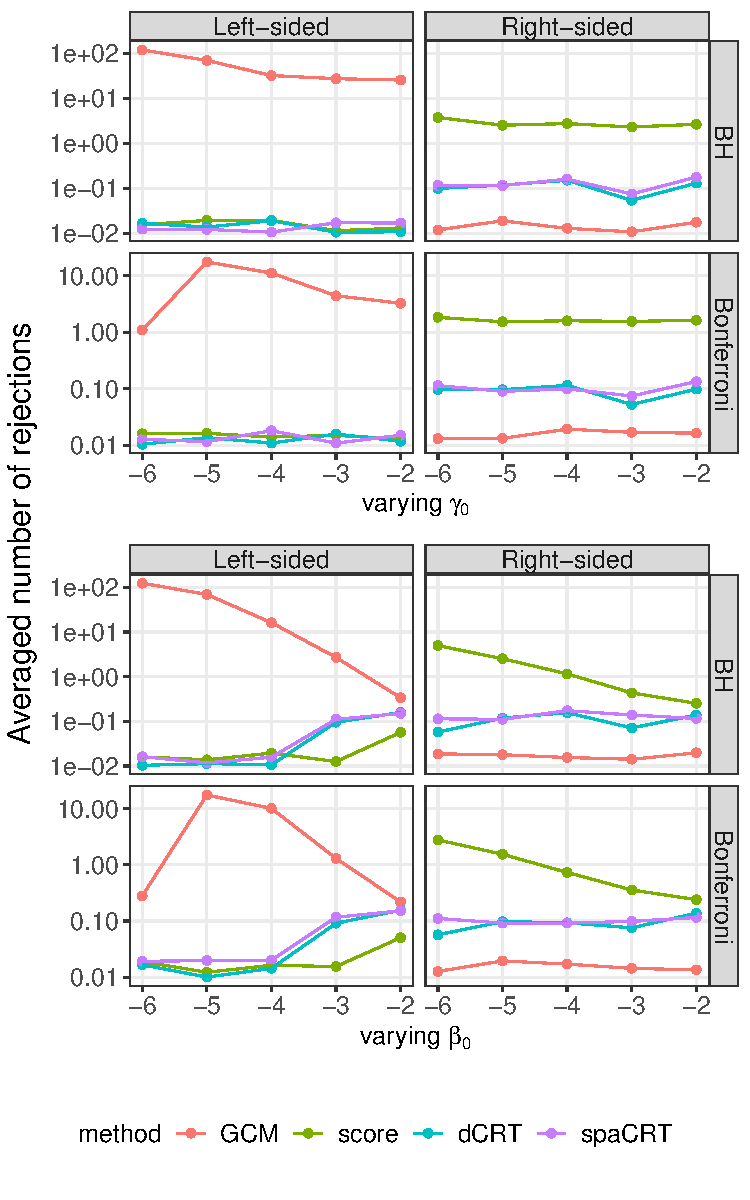
\includegraphics[width=0.8\textwidth]{figures-and-tables/simulation/NB-regression/FDR/disp-0.05-multiple_testing_rejection_plot.pdf}
    \caption{Averaged number of rejections after BH and Bonferroni corrections under the setup $r=0.05$.}
    \label{fig:simulation-CRISPR-screens-high-multiplicity-disp-0.05}
  \end{figure}

  \begin{figure}[!ht]
	\centering
	\begin{subfigure}{\textwidth}
		\centering
		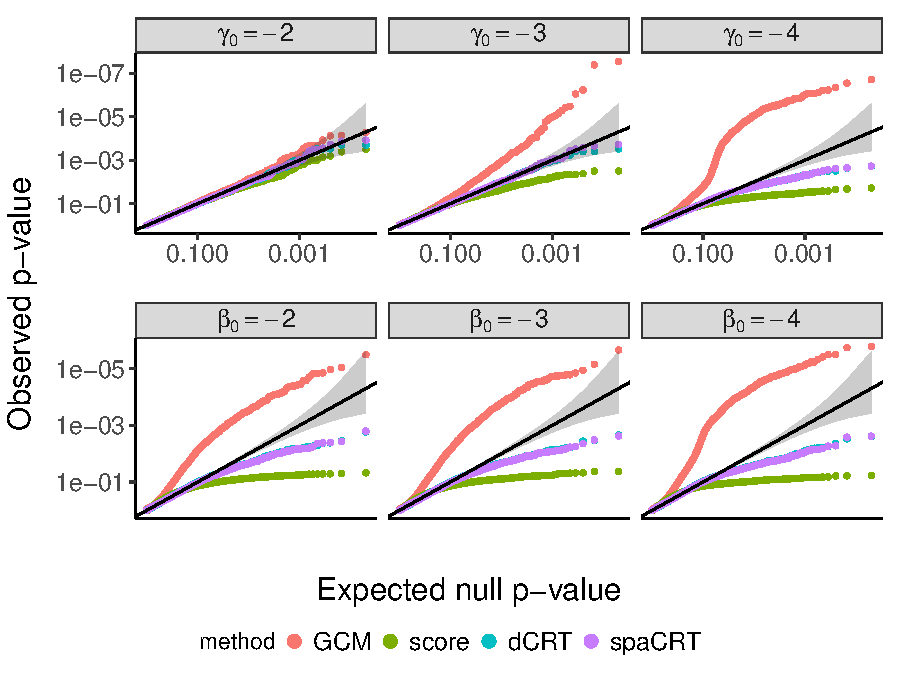
\includegraphics[width=0.95\textwidth]{figures-and-tables/simulation/NB-regression/QQ/disp-0.05-QQ-LEFT.pdf}
	\end{subfigure}

	\begin{subfigure}{\textwidth}
		\centering
		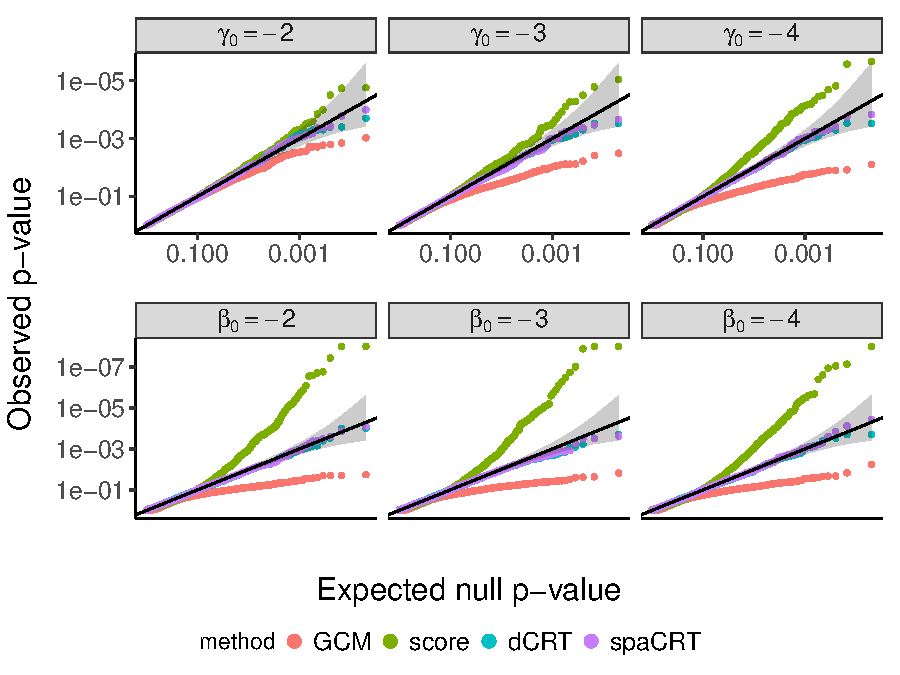
\includegraphics[width=0.95\textwidth]{figures-and-tables/simulation/NB-regression/QQ/disp-0.05-QQ-RIGHT.pdf}
	\end{subfigure}
	\caption{QQ plots of the $p$-values when $r=0.05$. Top: left-sided test. Bottom: right-sided test. }
	\label{fig:simulation-CRISPR-screens-disp-0.05-QQ}
  \end{figure}
  

  \begin{figure}[!ht]
	\centering
	\begin{subfigure}{\textwidth}
		\centering
		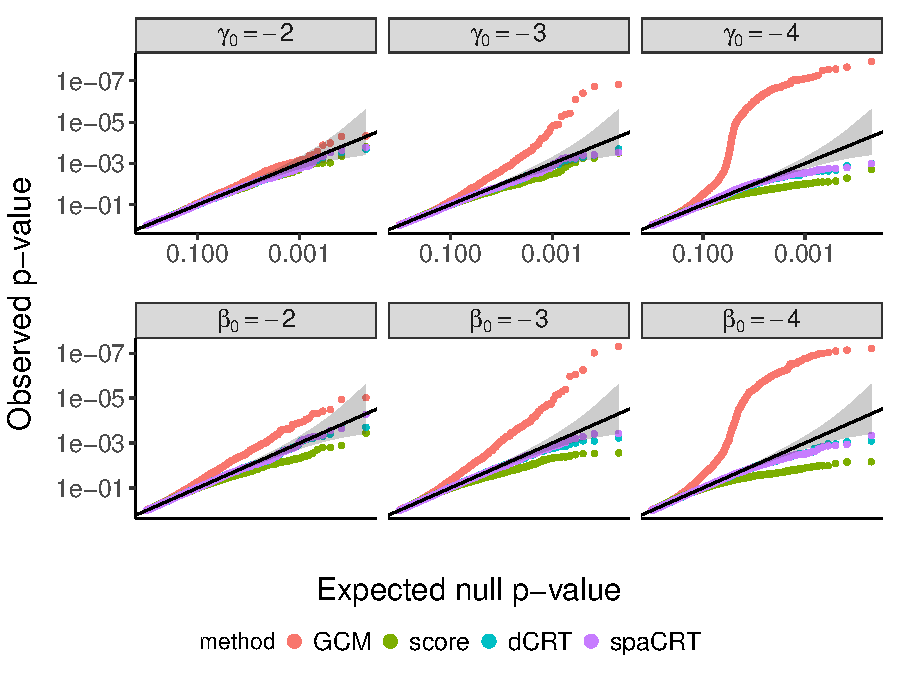
\includegraphics[width=0.95\textwidth]{figures-and-tables/simulation/NB-regression/QQ/disp-1-QQ-LEFT.pdf}
	\end{subfigure}

	\begin{subfigure}{\textwidth}
		\centering
		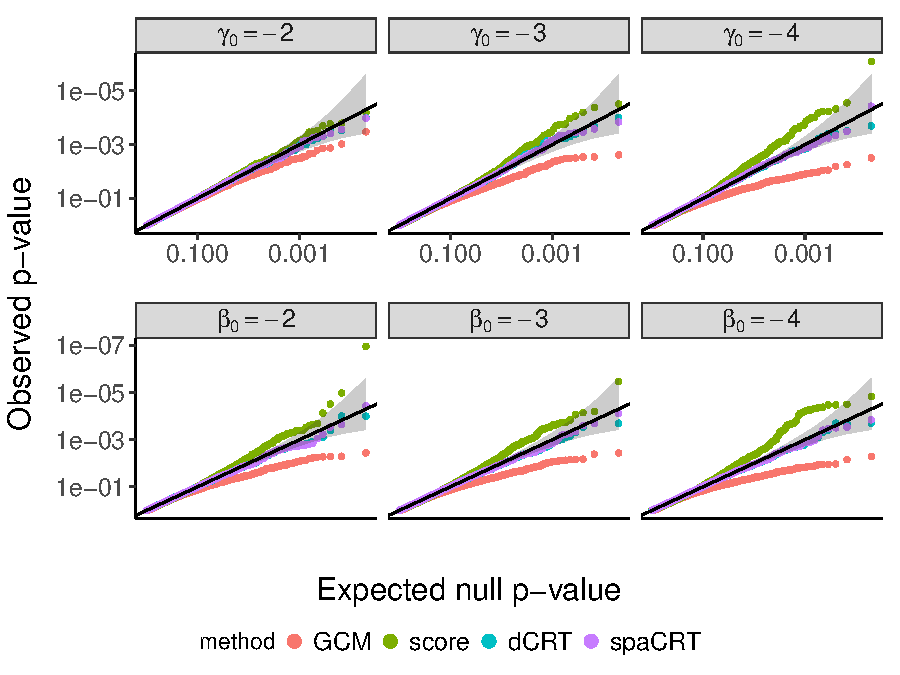
\includegraphics[width=0.95\textwidth]{figures-and-tables/simulation/NB-regression/QQ/disp-1-QQ-RIGHT.pdf}
	\end{subfigure}
	\caption{QQ plots of the $p$-values when $r=1$. Top: left-sided test. Bottom: right-sided test. }
	\label{fig:simulation-CRISPR-screens-disp-1-QQ}
  \end{figure}


  \begin{figure}[!ht]
	\centering
	\begin{subfigure}{\textwidth}
		\centering
		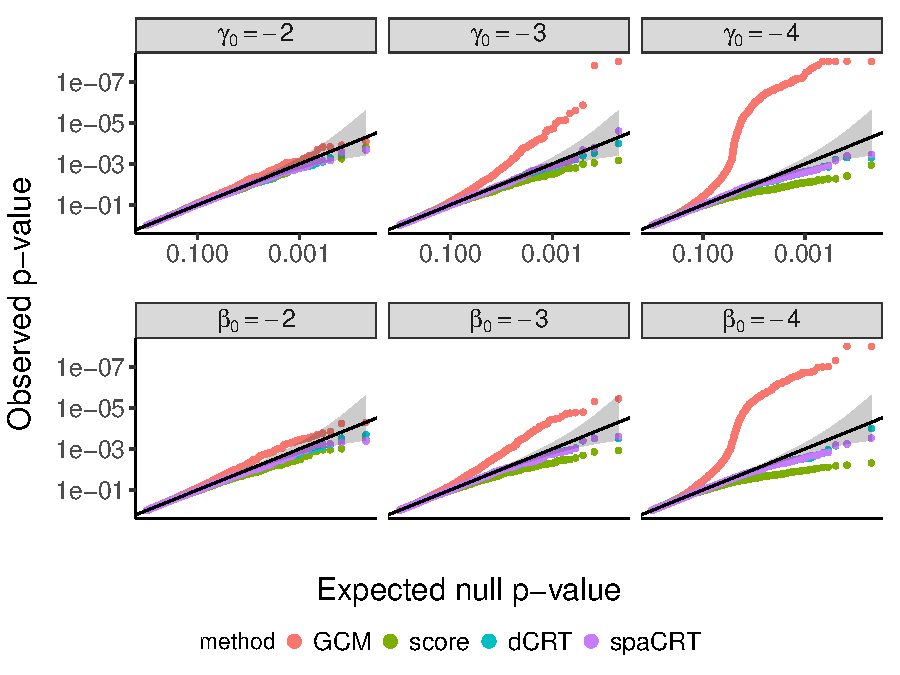
\includegraphics[width=0.95\textwidth]{figures-and-tables/simulation/NB-regression/QQ/disp-10-QQ-LEFT.pdf}
	\end{subfigure}

	\begin{subfigure}{\textwidth}
		\centering
		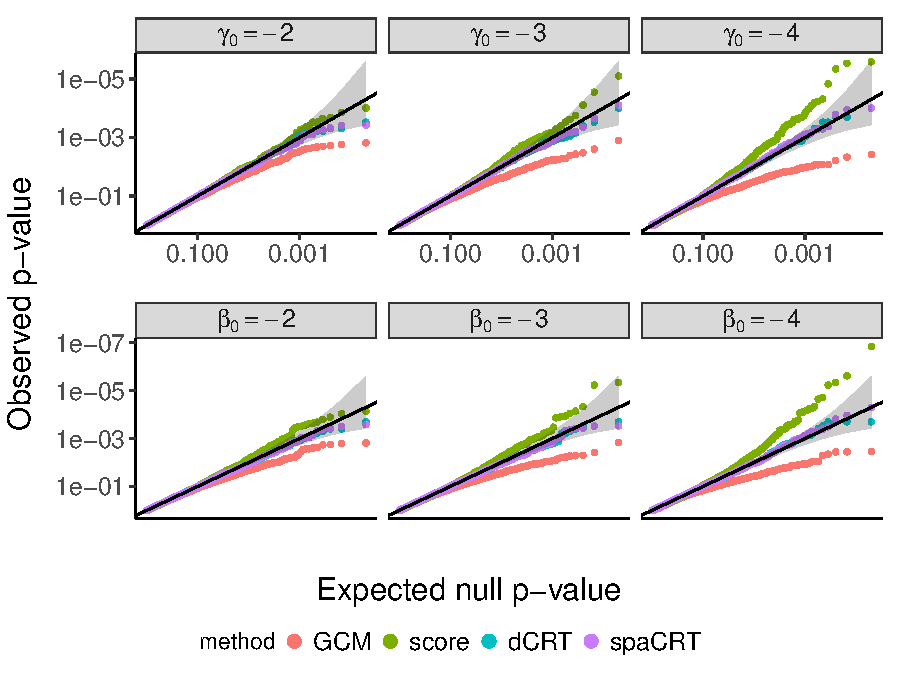
\includegraphics[width=0.95\textwidth]{figures-and-tables/simulation/NB-regression/QQ/disp-10-QQ-RIGHT.pdf}
	\end{subfigure}
	\caption{QQ plots of the $p$-values when $r=10$. Top: left-sided test. Bottom: right-sided test. }
	\label{fig:simulation-CRISPR-screens-disp-10-QQ}
  \end{figure}
  

  \begin{figure}[!ht]
	\centering
	\begin{subfigure}{\textwidth}
		\centering
		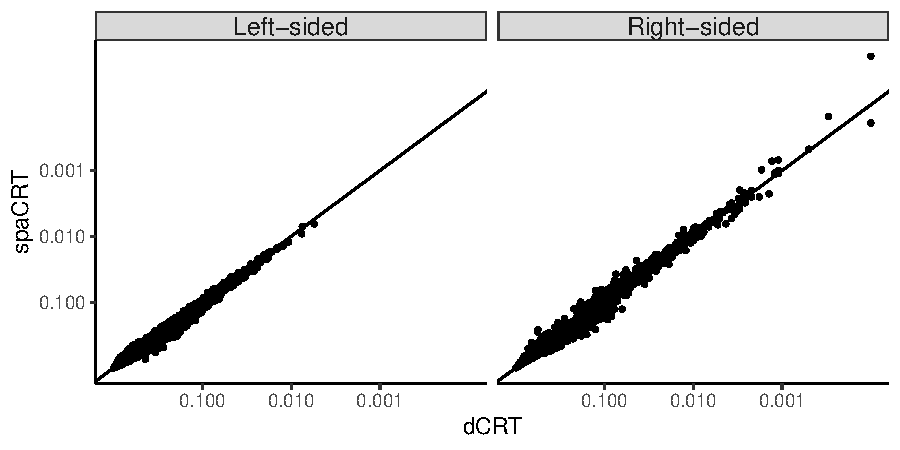
\includegraphics[width=.95\textwidth]{figures-and-tables/simulation/NB-regression/QQ/disp-0.05-dCRT-spaCRT.pdf}
	\end{subfigure}

	\begin{subfigure}{\textwidth}
		\centering
		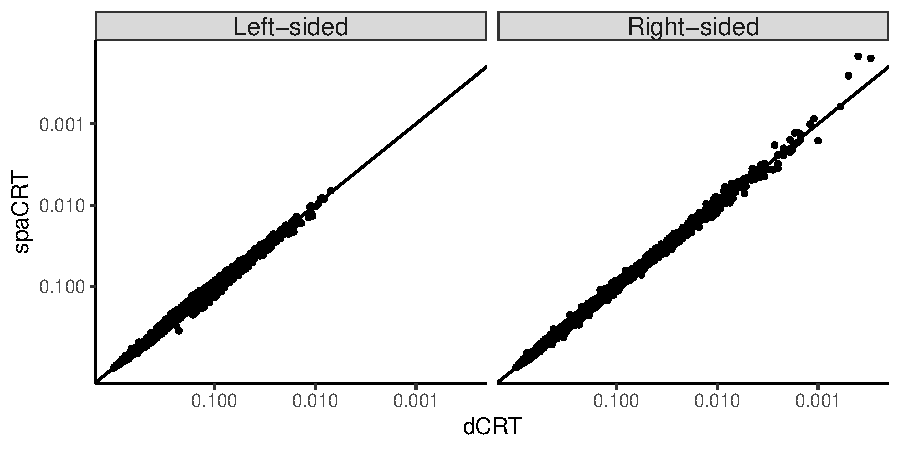
\includegraphics[width=.95\textwidth]{figures-and-tables/simulation/NB-regression/QQ/disp-1-dCRT-spaCRT.pdf}
	\end{subfigure}

	\begin{subfigure}{\textwidth}
		\centering
		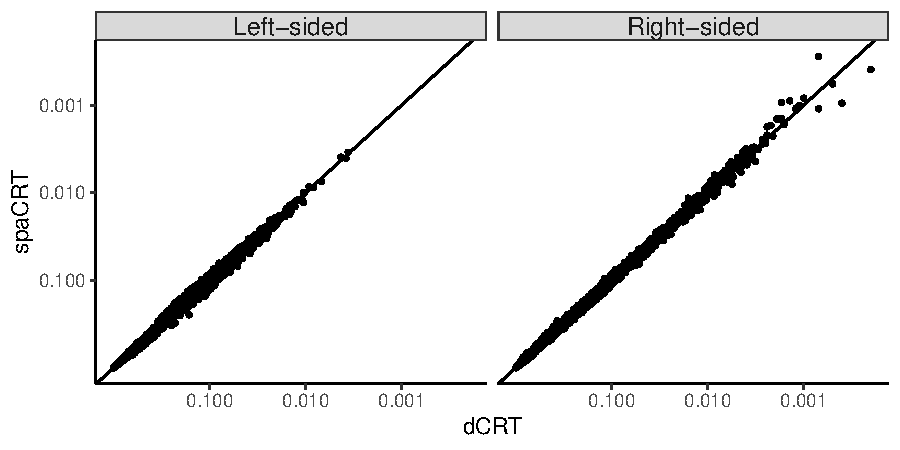
\includegraphics[width=.95\textwidth]{figures-and-tables/simulation/NB-regression/QQ/disp-10-dCRT-spaCRT.pdf}
	\end{subfigure}

    \caption{$p$-value approximation accuracy of $\spacrt$ and $\dCRT$ when $r=0.05, 1, 10$. Top: $r=0.05$. Middle: $r=1$. Bottom: $r=10$.}
    \label{fig:simulation-CRISPR-screens-approximation-accuracy}
  \end{figure}

\clearpage

\section{Additional simulation details in Section \ref{sec:GWAS}}\label{sec:additional_details_GWAS}

\subsection{Source of sparsity in GWAS with rare phenotypes}\label{sec:source_sparsity_GWAS}

GWAS aim to investigate if genetic variation is associated with a phenotype of interest. There can be two sources of sparsity in such analysis. On one hand, the phenotype of interest ($Y$) can be rare, i.e. only a small fraction of the population has the phenotype. Typical examples include certain rare diseases which have low prevalence in the population. On the other hand, the sparsity can come from the rare genetic variation ($X$), i.e., only a small fraction of the population has the genetic variation. 


\subsection{Parameters and methods implementation in Section \ref{sec:GWAS}}\label{sec:simulation_methods_GWAS}

\paragraph{Parameters used in Section \ref{sec:GWAS}.}
Recall the logistic regression model:
\begin{align*}
	\law(\pry|\prx)\overset{d}{=}\text{Ber}(\expit(\gamma_0 + \prx^\top \beta))
\end{align*}
where $\gamma_0$ is an intercept term, $\beta$ is a vector of coefficient and $g$ is a smooth function. For the concrete choice of $\beta$, we consider 
\begin{align*}
	\beta = (\underbrace{\eta,\ldots,\eta}_{0.05 * p},\underbrace{-\eta,\ldots,-\eta}_{0.05 * p},\underbrace{0,\ldots,0}_{0.9 * p})^\top
\end{align*}
where $\eta>0$ is a signal strength. We vary $\eta\in\{0, 0.25, 0.5, 0.75, 1\}$. For $\gamma_0$, we consider $\{-3,-2\}$ for \textit{high} and \textit{low} sparsity settings. For the distribution of $\prx$, we consider the mHHM (Definition \ref{def:mhhm}) where we consider $\pru_j\in\{1,2,\ldots,10\}$ and $\prx\in\{0,1\}$. Therefore $K=10$ and $M=2$. The Markov transition matrix is 
\begin{align*}
	Q\equiv 
	\begin{pmatrix}
		\gamma & 1-\gamma & 0 & \ldots & 0 & 0\\
		0 & \gamma & 1-\gamma & \ldots & 0 & 0\\
		\vdots & &  \ddots & & &\vdots\\
		\vdots & &  & \ddots & &\vdots\\
		0 & 0 & 0 & \ldots & \gamma & 1 - \gamma\\
		0 & 0 & 0 & \ldots & 0 & 1\\
	\end{pmatrix}
	\in\mathbb{R}^{K\times K}.
\end{align*}
We set $\gamma=0.9$ to create non-trivial correlation between $\prx_j$. The intial distribution $q$ is a uniform distribution over the support of $\pru_1$. Besides the transition matrix, we also vary the emission distribution $\prx_j|\pru_j$ by considering a beta-piror emission distribution:
\begin{align}\label{eq:beta_emission}
  \P[\prx_j=1|\pru_j=k]\overset{\mathrm{i.i.d.}}{\sim} \mathrm{Beta}(\alpha,\beta).
  \tag{beta-emission}
\end{align}
Hyperparameter $(\alpha,\beta)$ controls the shape of the Beta distribution. We consider two choices: $(\alpha,\beta)=(1,3)$ and $(\alpha,\beta)=(1,1)$. The first set of parameters will put more mass towards small values close to $0$, which induce high sparsity and thus mimic the rare genetic variation setup. The second choice is a uniform distribution over $[0,1]$ with no skewness. Thus this choice will induce low sparsity in $X$ and thus mimic the common genetic variation scenario. The simulation setup can be summarized in Table \ref{tab:simulation_parameter_GWAS}.

\begin{table}[!ht]
  \centering
  \caption{\label{tab:simulation_parameter_GWAS}Parameters considered in GWAS simulation.}
  \centering
  \begin{tabular}[t]{cc}
  \toprule
  Parmeters $((\alpha,\beta),\gamma_0)$ & Sparsity level for $(X,Y)$\\
  \midrule
  $((1,3),-2)$ & (high, low) \\
  $((1,3),-3)$ & (high, high) \\
  $((1,1),-2)$ & (low, low) \\
  $((1,1),-3)$ & (low, high) \\
  \bottomrule
  \end{tabular}
\end{table}
\noindent We will consider regularization parameters $\lambda$ used in \texttt{glmnet} to be $\lambda=\texttt{lambda.1se}$ or $\lambda=\texttt{lambda.min}$. 


\paragraph{Methods details for Section \ref{sec:GWAS}.}


\begin{itemize}
  \item The \textbf{spaCRT} (Algorithm~\ref{alg:spacrt}), where the parameters of the HMM are fitted based on expectation-maximization (EM) algorithm implemented by \texttt{fastPhase} software \citep{scheet2006fast}. \texttt{fastPhase} has also been a popular method in the recent variable selection literatures \citep{sesia2019gene}. Conditional distribution $\pry \mid \prx_j$ is fitted based on a modified high-dimensional logistic regression with lasso penalization \citep{tibshirani1996regression}, using the tower trick. We refer the details of methods implementation to Appendix~\ref{sec:tower-trick}.
  \item The \textbf{Knockoffs} \citep{barber2015controlling,sesia2019gene}, where the distribution of $\prx$ is fitted in the same way as in $\spacrt$ and knockoff variables are constructed via backford sampling algorithm proposed in \citet{sesia2019gene}. The test statistic is chosen to be the difference of absolute coefficient values between the variable of interest $\prx_j$ and its corresponding knockoff variable $\tilde \prx_j$, which are obtained in the high-dimensional logistic regression with lasso penalization for fitting $\pry|\prx,\tilde \prx$, where $\tilde\prx=(\tilde \prx_1,\ldots,\tilde \prx_d)^\top\in\mathbb{R}^d$.
\end{itemize}
We also include \textbf{dCRT} (Algorithm~\ref{alg:dcrt-hat}) with resample $M = 5000$ and \textbf{GCM test} \citep{Shah2018}, with the same fitting procedures as the $\spacrt$. 

\subsection{Tower-trick for spaCRT, dCRT and GCM}\label{sec:tower-trick}

We will discuss a simple yet powerful computational trick to compute the leave-one-out conditional expectations $\widehat \E[\pry|\prx_{-j}]$ for $\dCRT,\spacrt$ and $\GCM$. We first observe the following identity:
\begin{align*}
	\E[\pry|\prx_{-j}]=\E[\E[\pry|\prx]|\prx_{-j}]
\end{align*}
where the outer expectation is taken with respect to the measure $\prx_j|\prx_{-j}$. If we can estimate the joint distribution of $\prx$ from data $X$ and one regression estimate for $\E[\pry|\prx]$, computing the conditional expectation $\E[\pry|\prx_{-j}]$ for any $j\in[d]$ is straightforward via the integral evaluation with respect to measure $\prx_j|\prx_{-j}$, without any additional regression fit. In other words, we only need one regression fit for $\E[\pry|\prx]$ and one joint distribution fit for $\prx$. In practice, we consider using the following algorithm:
\begin{enumerate}
  \item \textbf{Estimate distribution $\prx$:} this can be done by using \texttt{fastPhase} \citep{scheet2006fast};
  \item \textbf{Compute regression estimate $\widehat \E[\pry|\prx=x]$:} this can be done by using \texttt{glmnet} \citep{tibshirani1996regression} with the family set to be \texttt{binomial};
  \item \textbf{Compute $\widehat\E[\pry|\prx_{-j}]$ for any $j\in[d]$:} this can be done by computing the following integral:
  \begin{align*}
    \widehat\E[\pry|\prx_{-j}=x_{-j}]=\sum_{x_j\in\{0,1\}}\widehat\E[\pry|\prx=x]\widehat \P[\prx_j=x_j|\prx_{-j}=x_{-j}],
  \end{align*}
  where $\widehat{\P}[\prx_j=x_j|\prx_{-j}=\cdot]$ is estimated using the \texttt{fastPhase} algorithm.
\end{enumerate}


\subsection{Additional simulation results in Section \ref{sec:GWAS}}\label{sec:simulation_results_GWAS}

We present additional simulation results in this section.  The results can be found in Figure~\ref{fig:simulation-summary-GWAS-uniform-lambda-1se}, \ref{fig:simulation-summary-GWAS-uniform-lambda-min} and \ref{fig:simulation-summary-GWAS-skew-lambda-min}. We want to point out that the choice of regularization parameter $\lambda$ seems to affect both the FDR and power of the methods. In particular, comparing Figure~\ref{fig:simulation-summary-GWAS-uniform-lambda-1se} and Figure~\ref{fig:simulation-summary-GWAS-uniform-lambda-min}, we can find the FDR can be slightly inflated when \texttt{lambda.min} is used for $\dCRT,\GCM$ and $\spacrt$ methods whereas the FDR is well controlled when \texttt{lambda.1se} is used. The inflation of false positive rate can be because of the tower trick used for these methods. The intuition is that when \texttt{lambda.1se} is used for $\dCRT,\GCM$ and $\spacrt$, the estimated regression coefficients are more sparse and the models obtained from \texttt{glmnet} is less variable whereas \texttt{lambda.min} will lead to more variable models due to the relatively dense model it will produce. On the power side, we can see that the power of $\dCRT,\GCM$ and $\spacrt$ is slightly improved when \texttt{lambda.min} is used. Interestingly, the FDR of Knockoff procedure seems to be more robust to the choice of $\lambda$ whereas the power is worse when \texttt{lambda.min} is used, which is different from the behavior of $\dCRT,\GCM$ and $\spacrt$. 

\begin{figure}[!ht]
  \centering
  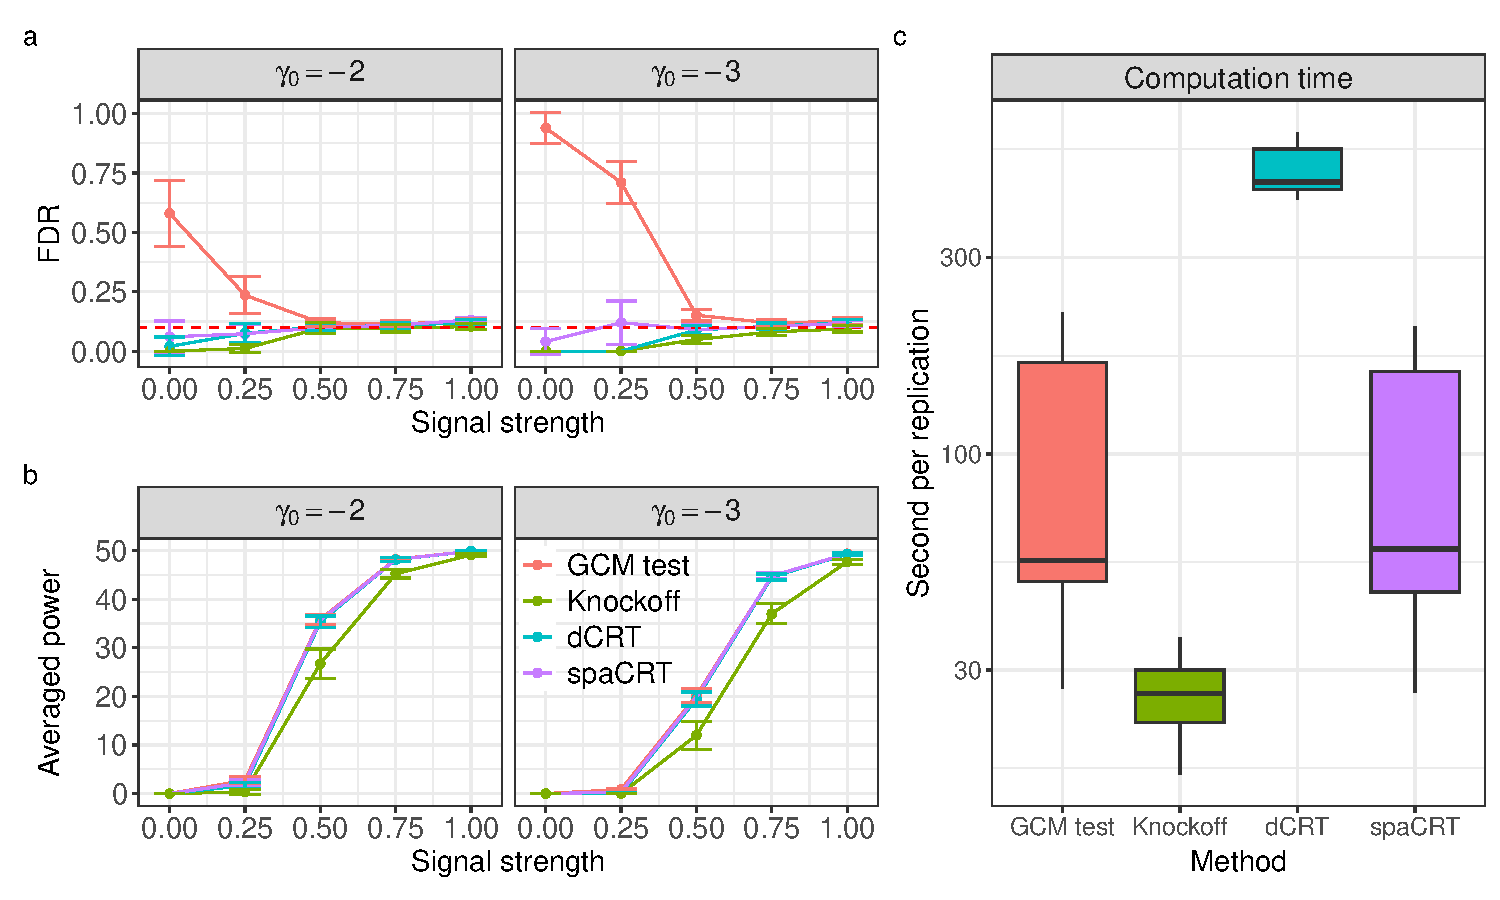
\includegraphics[width=1.0\textwidth]{figures-and-tables/simulation/HMM-variable-selection/HMM_simulation_uniform_lambda.1se.pdf}
  \caption{Summary of numerical simulation results for variable selection  with $(\alpha,\beta)=(1,1)$ and $\lambda=\texttt{lambda.1se}$. (a) FDR for $\gamma_0=-3$ (high sparsity) and $\gamma_0=-2$ (low sparsity). (b) Power for the same set of $\gamma_0$. (c) Computation times by different methods. }
  \label{fig:simulation-summary-GWAS-uniform-lambda-1se}
\end{figure}

\begin{figure}[!ht]
  \centering
  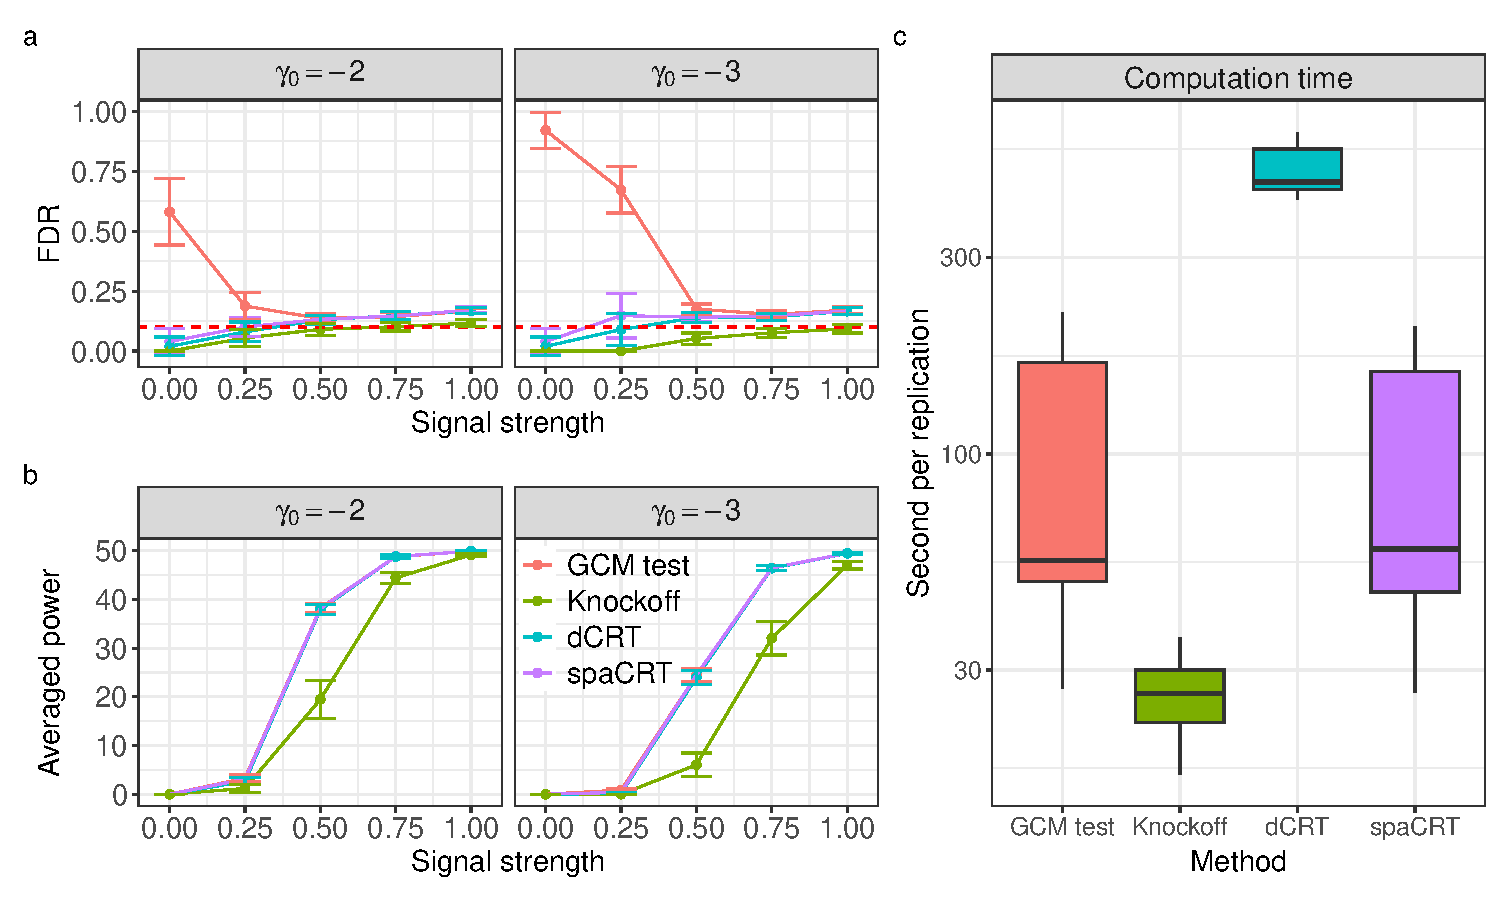
\includegraphics[width=1.0\textwidth]{figures-and-tables/simulation/HMM-variable-selection/HMM_simulation_uniform_lambda.min.pdf}
  \caption{Summary of numerical simulation results for variable selection with $(\alpha,\beta)=(1,1)$ and $\lambda=\texttt{lambda.min}$. (a) FDR for $\gamma_0=-3$ (high sparsity) and $\gamma_0=-2$ (low sparsity). (b) Power for the same set of $\gamma_0$. (c) Computation times by different methods. }
  \label{fig:simulation-summary-GWAS-uniform-lambda-min}
\end{figure}


\begin{figure}[!ht]
  \centering
  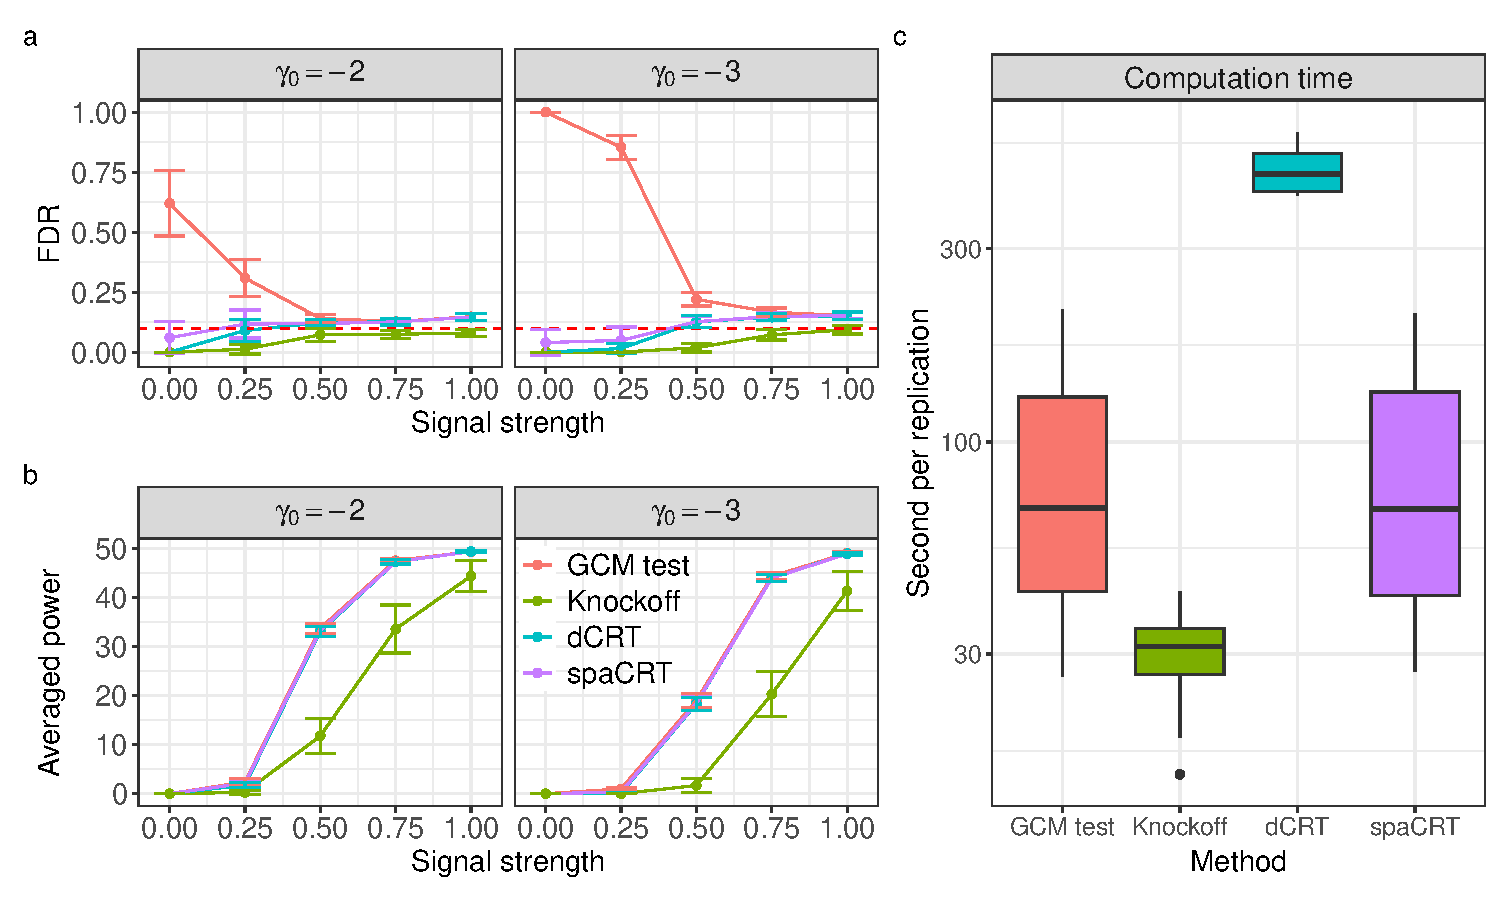
\includegraphics[width=1.0\textwidth]{figures-and-tables/simulation/HMM-variable-selection/HMM_simulation_skew_lambda.min.pdf}
  \caption{Summary of numerical simulation results for variable selection with $(\alpha,\beta)=(1,3)$ and $\lambda=\texttt{lambda.min}$. (a) FDR for $\gamma_0=-3$ (high sparsity) and $\gamma_0=-2$ (low sparsity). (b) Power for the same set of $\gamma_0$. (c) Computation times by different methods. }
  \label{fig:simulation-summary-GWAS-skew-lambda-min}
\end{figure}

\clearpage


\section{Additional figures and tables for real data analysis}

We present relevant information about Gasperinit dataset in Section~\ref{sec:additional-details-real-data}. In Section \ref{sec:additional_table_realdata}, we show a table including the number of rejections when applying Bonferroni or BH method to the pairs invlovling the non-targeting perturbations (thus under the null). The total number of hypotheses is $153000$. In Section~\ref{sec:additional_figure_realdata}, we present additional figures for real data analysis including QQ-plots faceting across different effective sample size (Figure \ref{fig:qqplot_lowess}) and QQ-plots faceting across different dispersion parameters (Figure \ref{fig:qqplot_dispersion}). We report the failure of $\spacrt$ occurring in at most $0.007 \%$ of all hypotheses tested. 



\subsection{Overview of the data}\label{sec:additional-details-real-data}

The Gasperini data contain expression measurements on 13,135 genes and CRISPR perturbations targeting 6,105 regulatory elements in $n =$ 207,324 cells. They also contain CRISPR perturbations intended as negative and positive controls. In particular, the data contain 51 non-targeting CRISPR perturbations, which do not target any regulatory element and therefore should have no effect on the expressions of any genes. Furthermore, the data contain 754 CRISPR perturbations targeting genes, rather than regulatory elements. These serve as positive controls, because they are known a priori to have effects on the expressions of the genes they target. Finally, the data contain measurements on six covariates, including four count-based covariates related to library size, one binary covariate indicating the experimental batch, and one continuous covariate indicating the proportion of reads mapping to mitochondrial genes in each cell.

\subsection{Data sparsity}\label{sec:sparsity_level_realdata}

To demonstrate that the sparsity in the real data, Figure~\ref{fig:sparsity-histograms} summarizes the sparsity of gRNA presence and gene expression in our real single-cell CRISPR dataset. Panel a shows that many genes exhibit expression rates near \(0.01\), while Panel b shows that gRNA perturbation presence are generally even lower. We also show the effective sample size of the 153,000 negative control pairs in Table~\ref{tab:sparsity_level_ess}. We comment that the sparsity in real data roughly matches what we chose in the simulation (see Section~\ref{sec:simulation_methods_CRISPR_screens}). The effective sample size is defined as the number of cells in which both the gRNA and gene expression are non-zero.  

\begin{figure}[!ht]
	\centering
	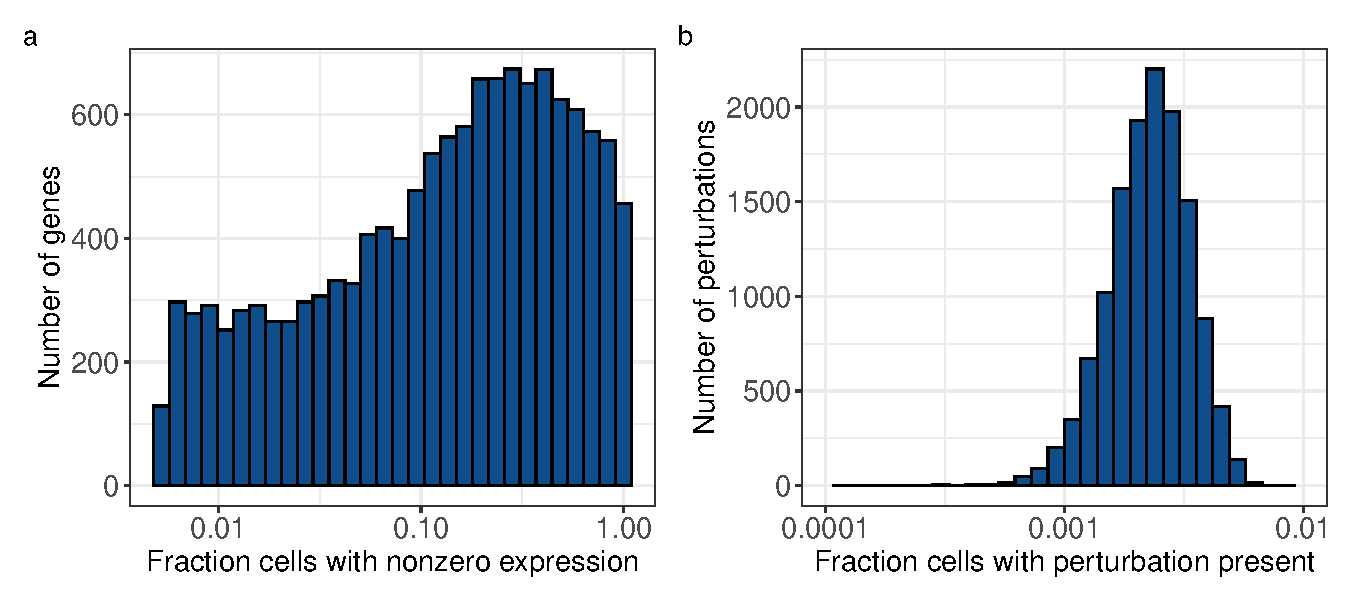
\includegraphics[width=1.0\textwidth]{figures-and-tables/real-data/sparsity_histograms.pdf}
	\caption{Histograms of the sparsity in \citet{Gasperini2019a}. (a) The histogram of the sparsity of gene expression. (b) The histogram of the sparsity of gRNA presence.}
	\label{fig:sparsity-histograms}
\end{figure}

  
\begin{table*}[h!]
	\centering
	\begin{tabular}[t]{lccccc}
	\toprule
	  & Min. & 1st Qu. & Median & 3rd Qu. & Max.\\
	\midrule
	Effective sample size & 0   &   53   &  204  &   504  & 2044 \\
	\bottomrule
	\end{tabular}
	\caption{Effective sample sizes in the 153,000 negative control pairs.}
	\label{tab:sparsity_level_ess}
\end{table*}


\subsection{Additional table for the real data analysis}\label{sec:additional_table_realdata}

\begin{table}[!h]
\centering
\caption{\label{tab:real_data_rejection}Number of rejections for negative control pairs on the Gasperini data.}
\centering
\begin{tabular}[t]{lrrrr}
\toprule
\multicolumn{1}{c}{ } & \multicolumn{4}{c}{Number of rejections} \\
\cmidrule(l{3pt}r{3pt}){2-5}
\multicolumn{1}{c}{ } & \multicolumn{2}{c}{Left-sided test} & \multicolumn{2}{c}{Right-sided test} \\
\cmidrule(l{3pt}r{3pt}){2-3} \cmidrule(l{3pt}r{3pt}){4-5}
\multicolumn{1}{c}{Method} & \multicolumn{1}{c}{Bonferroni} & \multicolumn{1}{c}{BH} & \multicolumn{1}{c}{Bonferroni} & \multicolumn{1}{c}{BH} \\
\cmidrule(l{3pt}r{3pt}){1-1} \cmidrule(l{3pt}r{3pt}){2-2} \cmidrule(l{3pt}r{3pt}){3-3} \cmidrule(l{3pt}r{3pt}){4-4} \cmidrule(l{3pt}r{3pt}){5-5}
GCM test & 22 & 128 & 0 & 0\\
Score test & 1 & 1 & 15 & 29\\
spaCRT & 1 & 1 & 0 & 0\\
dCRT & 1 & 4 & 0 & 0\\
\bottomrule
\end{tabular}
\end{table}


\newpage

\subsection{Additional figures for the real data analysis}\label{sec:additional_figure_realdata}

\begin{figure*}[!ht]
	\centering
	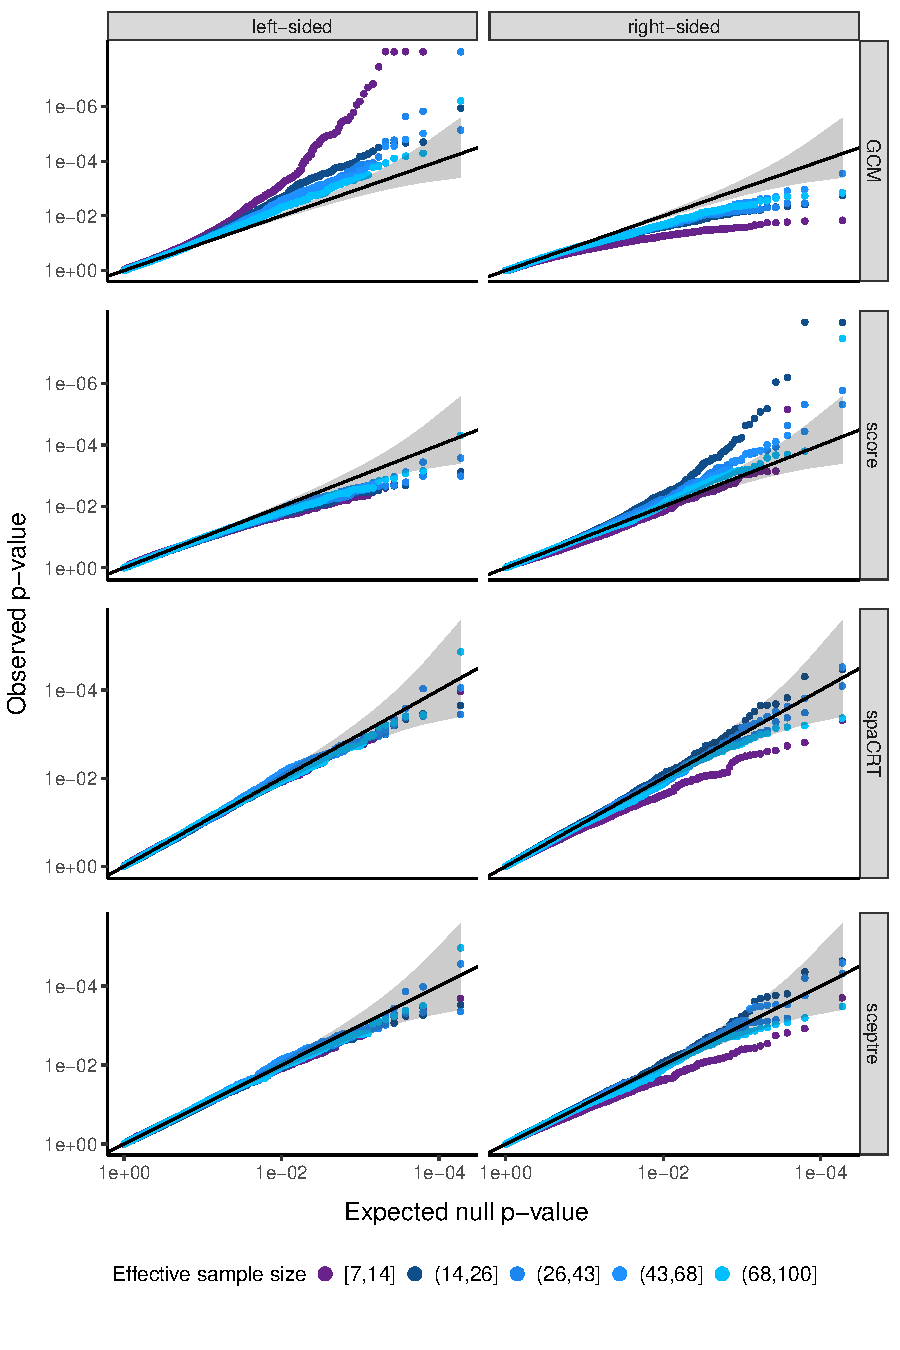
\includegraphics[width=0.95\textwidth]{figures-and-tables/real-data/facet_plot_different_withglmnb_100.pdf}
	\caption{QQ-plots for the $p$-values of right-sided test from different methods under low effective sample size.}
	\label{fig:qqplot_lowess}
\end{figure*}

\begin{figure*}[!ht]
	\centering
	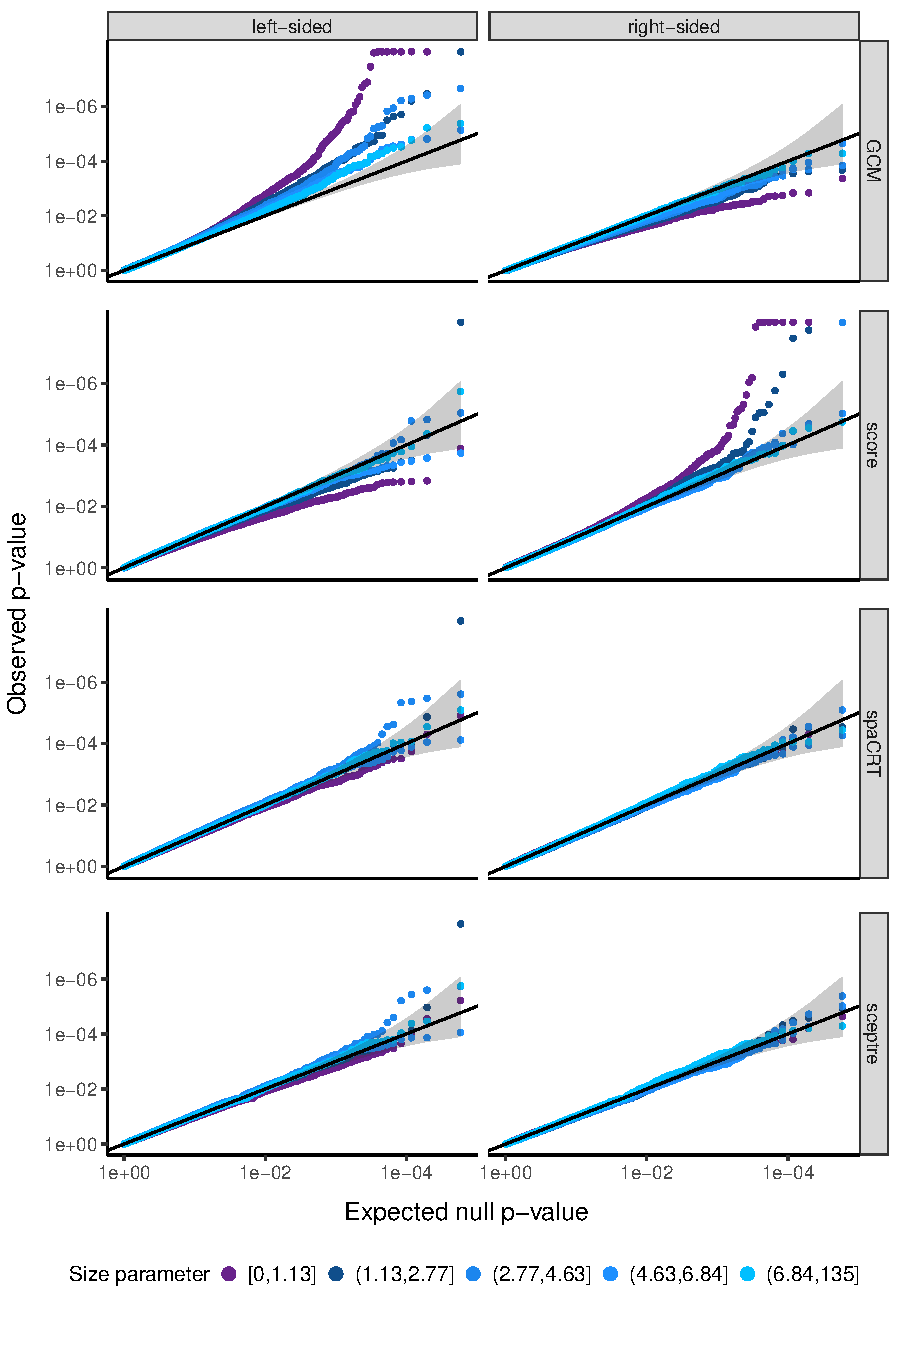
\includegraphics[width=0.95\textwidth]{figures-and-tables/real-data/facet_plot_different_withglmnb_dispersion.pdf}
	\caption{QQ-plots for the $p$-values of left-sided test from different methods stratified by dispersion parameter.}
	\label{fig:qqplot_dispersion}
\end{figure*}



\end{document}






















 




